%*********************************************************************
% Title: Business Research Methods
% Description: An Open Educational Resource for my BASV 316 class
% Author: George Self
% History: 
%   170101: Started This Puppy
%	170715: Re-started my work on this
%   180601: Re-started (again)
%   190206: I think that I finally finished the first (really rough) draft
%*********************************************************************

\RequirePackage{fix-cm} % fix some latex issues see: http://texdoc.net/texmf-dist/doc/latex/base/fixltx2e.pdf
\documentclass[ twoside, openright, titlepage, numbers=noenddot, headinclude,
  %1headlines, % letterpaper a4paper, 
  footinclude=true, cleardoublepage=empty, abstractoff, 
  % <--- obsolete, remove (todo)
  BCOR=5mm, 
  %paper=a4,
  paper=letter, fontsize=11pt,
  % ngerman (New German) formats German umlauts (among other things)
  american
  %
]{scrreprt}

%*********************************************************************
% Note: Make all your adjustments in here
%*********************************************************************
% *************************************************
% classicthesis-config.tex 
% Use it at the beginning of your ClassicThesis.tex, or as a LaTeX Preamble 
% in your ClassicThesis.{tex,lyx} with \input{classicthesis-config}
% *************************************************

% *************************************************
% 0. Set the encoding of your files. UTF-8 is the only sensible encoding nowadays. If you can't read
% äöüßáéçèê∂åëæƒÏ€ then change the encoding setting in your editor, not the line below. If your editor
% does not support utf8 use another editor!
% *************************************************
\PassOptionsToPackage{utf8}{inputenc}
  \usepackage{inputenc}

% *************************************************
% 1. Configure classicthesis for your needs here, e.g., remove "drafting" below 
% in order to deactivate the time-stamp on the pages
% *************************************************
\PassOptionsToPackage{eulerchapternumbers,listings,drafting,%
  pdfspacing,%floatperchapter,%linedheaders,%
  subfig,beramono,eulermath,parts}{classicthesis}

% *************************************************
% Available options for classicthesis.sty 
% (see ClassicThesis.pdf for more information):
% drafting
% parts nochapters linedheaders
% eulerchapternumbers beramono eulermath pdfspacing minionprospacing
% tocaligned dottedtoc manychapters
% listings floatperchapter subfig
% *************************************************

% *************************************************
% 2. Personal data and user ad-hoc commands
% *************************************************
\newcommand{\myTitle}{Research Methods\xspace}
\newcommand{\mySubtitle}{For Business and Marketing\xspace}
\newcommand{\myDegree}{Masters of Science\xspace}
\newcommand{\myName}{George Self\xspace}
\newcommand{\myProf}{Put name here\xspace}
\newcommand{\myOtherProf}{Put name here\xspace}
\newcommand{\mySupervisor}{Put name here\xspace}
\newcommand{\myFaculty}{Put data here\xspace}
\newcommand{\myDepartment}{Put data here\xspace}
\newcommand{\myUni}{University of South Arizona\xspace}
\newcommand{\myLocation}{Sierra Vista, AZ\xspace}
\newcommand{\myTime}{January, 2019\xspace}
\newcommand{\myVersion}{Edition 1\xspace}

% *************************************************
% Setup, finetuning, and useful commands
% *************************************************
\newcounter{dummy} % necessary for correct hyperlinks (to index, bib, etc.)
\newlength{\abcd} % for ab..z string length calculation
\providecommand{\mLyX}{L\kern-.1667em\lower.25em\hbox{Y}\kern-.125emX\@}
\newcommand{\ie}{i.\,e.}
\newcommand{\Ie}{I.\,e.}
\newcommand{\eg}{e.\,g.}
\newcommand{\Eg}{E.\,g.}
\newcommand{\etal}{\textit{et al}.}

% Create a blank page at the end of the document
\newcommand{\blankpage}{ 
	\newpage
	\thispagestyle{empty}
	\mbox{}
	\newpage
}

% The following creates a function named maxwidth that permits
% me to set a maximum width for images. If the natural width of
% the image is less than maxwidth then the image is rendered at
% its natural size, else scaled to maxwidth.
\makeatletter
\def\maxwidth#1{\ifdim\Gin@nat@width>#1 #1\else\Gin@nat@width\fi}
\makeatother

% *************************************************

% *************************************************
% My Packages
% *************************************************
\usepackage[
	type={CC},
	modifier={by-nc-sa},
	version={4.0}
]{doclicense} % Prints the Creative Commons license

\usepackage[obeyspaces,hyphens]{url}
\expandafter\def\expandafter\UrlBreaks\expandafter{\UrlBreaks%  save the current one
	\do\a\do\b\do\c\do\d\do\e\do\f\do\g\do\h\do\i\do\j%
	\do\k\do\l\do\m\do\n\do\o\do\p\do\q\do\r\do\s\do\t%
	\do\u\do\v\do\w\do\x\do\y\do\z\do\A\do\B\do\C\do\D%
	\do\E\do\F\do\G\do\H\do\I\do\J\do\K\do\L\do\M\do\N%
	\do\O\do\P\do\Q\do\R\do\S\do\T\do\U\do\V\do\W\do\X%
	\do\Y\do\Z}


% *************************************************

% *************************************************
% 3. Loading some handy packages
% *************************************************

% *************************************************
% Packages with options that might require adjustments
% *************************************************
%\PassOptionsToPackage{ngerman,american}{babel}   % change this to your language(s)
% Spanish languages need extra options in order to work with this template
%\PassOptionsToPackage{spanish,es-lcroman}{babel}
\usepackage{babel}

\usepackage{csquotes}

\PassOptionsToPackage{%
  backend=biber, %instead of bibtex
  backend=bibtex8,bibencoding=ascii,%
  language=auto,%
  style=numeric-comp,%
    %style=authoryear-comp, % Author 1999, 2010
    %bibstyle=authoryear,dashed=false, % dashed: substitute rep. author with ---
  sorting=nyt, % name, year, title
  maxbibnames=10, % default: 3, et al.
    %backref=true,%
  natbib=true % natbib compatibility mode (\citep and \citet still work)
  }{biblatex}
  \usepackage{biblatex}
\addbibresource{ResearchMethods}

% math environments and more by the AMS 
\PassOptionsToPackage{fleqn}{amsmath}  
  \usepackage{amsmath}

% *************************************************
% General useful packages
% *************************************************
\PassOptionsToPackage{T1}{fontenc} % T2A for cyrillics
  \usepackage{fontenc}
\usepackage{fontawesome}
\usepackage{textcomp} % fix warning with missing font shapes
\usepackage{scrhack} % fix warnings when using KOMA with listings package          
\usepackage{xspace} % to get the spacing after macros right  
\usepackage{mparhack} % get marginpar right
\usepackage{fixltx2e} % fixes some LaTeX stuff 

%\PassOptionsToPackage{printonlyused,smaller}{acronym} 
%  \usepackage{acronym} % nice macros for handling all acronyms in the thesis
%\renewcommand*{\aclabelfont}[1]{\acsfont{#1}}

\usepackage{shorttoc} % For the short TOC at the top of the document

% ***********************************************
% Used for wrapping figures
% ***********************************************
\usepackage{float}
\usepackage{wrapfig}
\restylefloat{figure}

% *************************************************
% 4. Setup tables, (sub)figures, and captions
% *************************************************
\usepackage[svgnames,table]{xcolor} % control row/cell color in a table
\usepackage{tabularx} % better tables
\usepackage{tabulary} % another tables option
\usepackage{multirow} % permits merging rows in a table
\setlength{\extrarowheight}{3pt} % increase table row height
\newcommand{\tableheadline}[1]{\multicolumn{1}{c}{\spacedlowsmallcaps{#1}}}
\newcommand{\myfloatalign}{\centering} % to be used with each float for alignment
\usepackage{tikz} % for drawing
\usetikzlibrary{positioning, arrows.meta, trees}
\usepackage{forest} % Draw decision trees

\usepackage{caption}
\captionsetup{font=small} % format=hang,
\usepackage{subfig}  

\usepackage{booktabs}
% *************************************************

% *************************************************
% Objectives boxes
% *************************************************
\usepackage{tcolorbox} % create nice color boxes
\definecolor{objgold}{RGB}{255,178,102}
\definecolor{tkawyblue}{RGB}{102,255,255}
\newtcolorbox{objbox}[1]{
	colback=objgold!5!white,
	colframe=objgold!85!black,
	fonttitle=\bfseries,
	width=.75\linewidth,
	title=#1}

\newtcolorbox{tkawybox}[1]{
	colback=tkawyblue!5!white,
	colframe=tkawyblue!70!black,
	fonttitle=\bfseries,
	width=.75\linewidth,
	title=#1}

% *************************************************
% 5. Setup code listings
% *************************************************
\usepackage{listings} 
\lstset{language=[LaTeX]Tex,%C++,
    morekeywords={PassOptionsToPackage,selectlanguage},
    keywordstyle=\color{RoyalBlue},%\bfseries,
    basicstyle=\small\ttfamily,
    %identifierstyle=\color{NavyBlue},
    commentstyle=\color{Green}\ttfamily,
    stringstyle=\rmfamily,
    numbers=none,%left,%
    numberstyle=\scriptsize,%\tiny
    stepnumber=5,
    numbersep=8pt,
    showstringspaces=false,
    breaklines=true,
    %frameround=ftff,
    %frame=single,
    belowcaptionskip=.75\baselineskip
    %frame=L
}
% *************************************************


% *************************************************
% Create a new command, blfootnote, that does not use 
% a footnote marker
% *************************************************
\newcommand\blfootnote[1]{%
	\begingroup
	\renewcommand\thefootnote{}\footnote{#1}%
	\addtocounter{footnote}{-1}%
	\endgroup
}

% *************************************************
% 6. PDFLaTeX, hyperreferences and citation backreferences
% *************************************************

% *************************************************
% Using PDFLaTeX
% *************************************************
\PassOptionsToPackage{pdftex,hyperfootnotes=false,pdfpagelabels}{hyperref}
  \usepackage{hyperref}  % backref linktocpage pagebackref
\pdfcompresslevel=9
\pdfadjustspacing=1 
\PassOptionsToPackage{pdftex}{graphicx}
  \usepackage{graphicx} 

% *************************************************
% Hyperreferences
% *************************************************
\hypersetup{%
  %draft, % = no hyperlinking at all (useful in b/w printouts)
  colorlinks=true, linktocpage=true, pdfstartpage=3, pdfstartview=FitV,%
  % uncomment the following line if you want to have black links (e.g., for printing)
  %colorlinks=false, linktocpage=false, pdfstartpage=3, pdfstartview=FitV, pdfborder={0 0 0},%
  breaklinks=true, pdfpagemode=UseNone, pageanchor=true, pdfpagemode=UseOutlines,%
  plainpages=false, bookmarksnumbered, bookmarksopen=true, bookmarksopenlevel=1,%
  hypertexnames=true, pdfhighlight=/O,%nesting=true,%frenchlinks,%
  urlcolor=webbrown, linkcolor=RoyalBlue, citecolor=webgreen, %pagecolor=RoyalBlue,%
  %urlcolor=Black, linkcolor=Black, citecolor=Black, %pagecolor=Black,%
  pdftitle={\myTitle},%
  pdfauthor={\textcopyright\ \myName, \myUni, \myFaculty},%
  pdfsubject={},%
  pdfkeywords={},%
  pdfcreator={pdfLaTeX},%
  pdfproducer={LaTeX with hyperref and classicthesis}%
}


% *************************************************
% Setup autoreferences
% *************************************************
% There are some issues regarding autorefnames
% http://www.ureader.de/msg/136221647.aspx
% http://www.tex.ac.uk/cgi-bin/texfaq2html?label=latexwords
% you have to redefine the makros for the 
% language you use, e.g., american, ngerman
% (as chosen when loading babel/AtBeginDocument)
% *************************************************
\makeatletter
\@ifpackageloaded{babel}%
  {%
    \addto\extrasamerican{%
    \renewcommand*{\figureautorefname}{Figure}%
    \renewcommand*{\tableautorefname}{Table}%
    \renewcommand*{\partautorefname}{Part}%
    \renewcommand*{\chapterautorefname}{Chapter}%
    \renewcommand*{\sectionautorefname}{Section}%
    \renewcommand*{\subsectionautorefname}{Section}%
    \renewcommand*{\subsubsectionautorefname}{Section}%     
  }%
\addto\extrasngerman
  {% 
    \renewcommand*{\paragraphautorefname}{Absatz}%
    \renewcommand*{\subparagraphautorefname}{Unterabsatz}%
    \renewcommand*{\footnoteautorefname}{Fu\"snote}%
    \renewcommand*{\FancyVerbLineautorefname}{Zeile}%
    \renewcommand*{\theoremautorefname}{Theorem}%
    \renewcommand*{\appendixautorefname}{Anhang}%
    \renewcommand*{\equationautorefname}{Gleichung}%        
    \renewcommand*{\itemautorefname}{Punkt}%
  }%  
% Fix to getting autorefs for subfigures right (thanks to Belinda Vogt for changing the definition)
\providecommand{\subfigureautorefname}{\figureautorefname}%             
  }{\relax}
\makeatother

% *************************************************
% Glossaries and Acronyms
% Note: Glossaries must be loaded after
% hyperref, babel, polyglossia, inputenc, and fontenc
% Note: I could never get glossaries to compile in this 
% document (but I could in another document). There doesn't
% seem to be a problem with MikTex or TexStudio, but
% some package I have installed for this document is not
% compatible with glossaries. I decided to just manually
% create a glossary in the ``Contents'' document.
% *************************************************
\usepackage[style=long,nolist]{glossaries}
\newcommand{\glossname}{Glossary}
\makeglossaries
\loadglsentries{AcroGloss}
%
%\newglossaryentry{LW}{name={Long Word},description={This is just a long word.}}
%
%\newacronym{wtf}{WTF}{What the Flying Freakin' Flip???}
% *************************************************
% 7. Last calls before the bar closes
% *************************************************
% *************************************************
% Development Stuff
% *************************************************
\listfiles
%\PassOptionsToPackage{l2tabu,orthodox,abort}{nag}
%   \usepackage{nag}
%\PassOptionsToPackage{warning, all}{onlyamsmath}
%   \usepackage{onlyamsmath}

% *************************************************
% Last, but not least...
% *************************************************
\usepackage{classicthesis} 
% *************************************************

% *************************************************
% 8. Further adjustments (experimental)
% *************************************************

% *************************************************
% Changing the text area
% *************************************************
%\linespread{1.05} % a bit more for Palatino
%\areaset[current]{312pt}{761pt} % 686 (factor 2.2) + 33 head + 42 head \the\footskip
%\setlength{\marginparwidth}{7em}%
%\setlength{\marginparsep}{2em}%

% *************************************************
% Using different fonts
% *************************************************
%\usepackage[oldstylenums]{kpfonts} % oldstyle notextcomp
%\usepackage[osf]{libertine}
%\usepackage[light,condensed,math]{iwona}
%\renewcommand{\sfdefault}{iwona}
%\usepackage{lmodern} % <-- no osf support :-(
%\usepackage{cfr-lm} % 
%\usepackage[urw-garamond]{mathdesign} <-- no osf support :-(
%\usepackage[default,osfigures]{opensans} % scale=0.95 
%\usepackage[sfdefault]{FiraSans}
% *************************************************


%*********************************************************************
% Bibliographies
%*********************************************************************
%\addbibresource{Bibliography.bib}
%\addbibresource[label=ownpubs]{AMiede_Publications.bib}

%*********************************************************************
% Hyphenation
%*********************************************************************
%\hyphenation{put special hyphenation here}

%*********************************************************************
% The document
%*********************************************************************
\begin{document}
\frenchspacing
\raggedbottom
\selectlanguage{american} % american ngerman
%\renewcommand*{\bibname}{new name}
%\setbibpreamble{}
\pagenumbering{roman}
\pagestyle{plain}
%*********************************************************************
% Frontmatter
%*********************************************************************
%%*******************************************************
% Little Dirty Titlepage
%*******************************************************
\thispagestyle{empty}
%\pdfbookmark[1]{Titel}{title}
%*******************************************************
\begin{center}
    \spacedlowsmallcaps{\myName} \\ \medskip                        

    \begingroup
        \color{Maroon}\spacedallcaps{\myTitle}
    \endgroup
\end{center}        

%*******************************************************
% Titlepage
%*******************************************************
\begin{titlepage}
    % if you want the titlepage to be centered, uncomment and fine-tune the line below (KOMA classes environment)
    \begin{addmargin}[-1cm]{-3cm}
    \begin{center}
        \large  

        \hfill

        \vfill

        \begingroup
            \color{Maroon}\spacedallcaps{\myTitle} \\ \bigskip
		        \mySubtitle \\ \medskip   
        \endgroup

        \spacedlowsmallcaps{\myName}

        \vfill

				% Adds a background image that covers entire page
				\tikz[remember picture,overlay] \node[opacity=0.3,inner sep=0pt] at (current page.center){
\includegraphics[width=\paperwidth,height=\paperheight]{gfx/coverart_v02}};

        \myTime\ -- \myVersion

        \vfill                      

    \end{center}  
  \end{addmargin}       
\end{titlepage}   
\thispagestyle{empty}

\hfill

\vfill

\noindent\myName: \textit{\myTitle,} \mySubtitle, \myTime 
%\myDegree, 

\doclicenseThis

%\textcopyright\ 

%\bigskip
%
%\noindent\spacedlowsmallcaps{Supervisors}: \\
%\myProf \\
%\myOtherProf \\ 
%\mySupervisor
%
%\medskip
%
%\noindent\spacedlowsmallcaps{Location}: \\
%\myLocation
%
%\medskip
%
%\noindent\spacedlowsmallcaps{Time Frame}: \\
%\myTime

%\cleardoublepage%*******************************************************
% Dedication
%*******************************************************
\thispagestyle{empty}
%\phantomsection 
\refstepcounter{dummy}
\pdfbookmark[1]{Dedication}{Dedication}

\vspace*{3cm}

\begin{center}
    \emph{Ohana} means family. \\
    Family means nobody gets left behind, or forgotten. \\ \medskip
    --- Lilo \& Stitch    
\end{center}

\medskip

\begin{center}
    Dedicated to the loving memory of Rudolf Miede. \\ \smallskip
    1939\,--\,2005
\end{center}
\cleardoublepage%************************************************
\chapter*{Foreword}\label{ch:foreword}
%************************************************
%TODO text draft done

I have taught BASV 316, \textit{Introductory Methods of Analysis}, online for the University of Arizona in Sierra Vista since 2010 and enjoy working with students on research methodology. I wanted a textbook that presented research in a practical way so students could use the lessons learned in their own research projects. I found an excellent book but over the years the cost of that book increased to the point that I felt like it was an unfair burden on students. 

I began by looking for an acceptable “open source” book since authors make those available to students free of charge and I could modify the book to meet my own objectives. I could not find any that were focused on business research though I tried for several years—and keep looking to this day. I did, though, find a few open source books about research in the social and psychological sciences that were reasonably close to what I needed. So, I modified those books to emphasize business research and then provided my work to students free of charge. 

The following books were the major sources for this book. They are all open source and published under a Creative Commons license that permitted me to copy and modify them.

\begin{itemize}
	\item Bhattacherjee, Anol, \textit{Social Science Research: Principles, Methods, and Practices}, found at \url{http://scholarcommons.usf.edu/oa_textbooks/3/}
	\item Blackstone, Amy, \textit{Principles of Sociological Inquiry: Qualitative and Quantitative Methods}, found at \url{https://open.umn.edu/opentextbooks/BookDetail.aspx?bookId=139}
	\item Price, Paul, \textit{Research Methods in Psychology}, found at \url{http://open.lib.umn.edu/psychologyresearchmethods/}. Note: this book was later updated by Price and posted in HTML format at \url{https://github.com/CrumpLab/ResearchMethods} 
\end{itemize}

Three goals shaped the choices made about the topics covered by the text and how those topics are presented. 

\begin{itemize}
	\item The topics must have relevance for business students. 
	\item Both qualitative and quantitative research methods are given roughly equal attention since both types of research are used in business. 
	\item The text is engaging and readable.
\end{itemize}

While the book is useful in its current form, I will continually update it based on emerging trends in research. 

This book is published under a Creative Commons \href{https://creativecommons.org/licenses/by-nc-sa/4.0/legalcode}{ Attribution-NonCommercial-ShareAlike} license, just like the books that provided its foundation. The source is available at my GitHub account: \url{http://bit.ly/2xIjzXL}. It is my hope that students can use this book to learn about business research and other instructors can modify and use it for their own classes.

\bigskip
\begin{flushright}
  \textemdash \; George Self
\end{flushright}

%\cleardoublepage%*******************************************************
% Abstract
%*******************************************************
%\renewcommand{\abstractname}{Abstract}
\pdfbookmark[1]{Abstract}{Abstract}
\begingroup
\let\clearpage\relax
\let\cleardoublepage\relax
\let\cleardoublepage\relax

\chapter*{Abstract}
Short summary of the contents in English\dots a great guide by 
Kent Beck how to write good abstracts can be found here:  
\begin{center}
\url{https://plg.uwaterloo.ca/~migod/research/beckOOPSLA.html}
\end{center}

\vfill

\begin{otherlanguage}{ngerman}
\pdfbookmark[1]{Zusammenfassung}{Zusammenfassung}
\chapter*{Zusammenfassung}
Kurze Zusammenfassung des Inhaltes in deutscher Sprache\dots 
\end{otherlanguage}

\endgroup			

\vfill
%\cleardoublepage%*******************************************************
% Publications
%*******************************************************
\pdfbookmark[1]{Publications}{publications}
\chapter*{Publications}\graffito{This is just an early --~and currently ugly~-- test!}
This might come in handy for PhD theses: some ideas and figures have appeared previously in the following publications:

%\noindent Put your publications from the thesis here. The packages \texttt{multibib} or \texttt{bibtopic} etc. can be used to handle multiple different bibliographies in your document.

\begin{refsection}[ownpubs]
    \small
    \nocite{*} % is local to to the enclosing refsection
    \printbibliography[heading=none]
\end{refsection}

\emph{Attention}: This requires a separate run of \texttt{bibtex} for your \texttt{refsection}, \eg, \texttt{ClassicThesis1-blx} for this file. You might also use \texttt{biber} as the backend for \texttt{biblatex}. See also \url{http://tex.stackexchange.com/questions/128196/problem-with-refsection}.
%\cleardoublepage%*******************************************************
% Acknowledgments
%*******************************************************
\chapter*{Acknowledgments}
This book was created from my original work and from several Open Educational Resources. I gratefully acknowledge the contribution from these sources:

%\begin{enumerate}
%%  \item Author Unknown, \textit{Introductory Statistics}, found at the Saylor.org site: \url{https://www.saylor.org/site/textbooks/Introductory Statistics.pdf}
%    
%  \item Author Unknown, \textit{Principles of Sociological Inquiry}, found at the Saylor.org site: \url{https://www.saylor.org/site/textbooks/Principles of Sociological Inquiry.pdf}
%    
%%  \item Author Unknown, \textit{Research Methods in Psychology}, found at the Saylor.org site: \url{https://www.saylor.org/site/textbooks/Research Methods in Psychology.pdf}
%  
%  \item Bhattacherjee, Anol, ``Social Science Research: Principles, Methods, and Practices'' (2012). \textit{Textbooks Collection}. Book 3.   \url{http://scholarcommons.usf.edu/oa\_textbooks/3}
%  
%\end{enumerate}

\begin{itemize}
	\item Amy Blackstone's book about Sociological Research found at saylor.org\footnote{Blackstone, A. "Principles of sociological inquiry: Qualitative and quantitative methods, v. 1.0 (pp. 236)." (2012).}.
	\item Anol Bhattacherjee's book about Social Science Research found at the University of Southern Florida's Scholar Commons\footnote{Bhattacherjee, Anol. "Social science research: Principles, methods, and practices." (2012).}.
\end{itemize}

All of these books and materials were published under a Creative Commons license which is often said to incorporate five R's:  

\begin{itemize}
	\item Reuse: I am using the two books to form my own work.
	\item Redistribute: My book is being freely distributed to my students and I've made it available to anyone else who wants to use it.
	\item Revise: I revised this book to include examples that are focused on research normally needed by business and marketing students rather than social science students.
	\item Remix: I mixed both books into one, removed the redundant parts, and added my own components.
	\item Retain: Students are able to retain a copy of this book until they choose to delete it.
\end{itemize}


\bigskip
\begin{flushright}
  \textemdash  George Self
\end{flushright}




\pagestyle{scrheadings}
\cleardoublepage%*******************************************************
% Table of Contents
%*******************************************************
%\phantomsection
\refstepcounter{dummy}

\shorttoc{Brief Contents}{0} % Only Chapters


\pdfbookmark[1]{\contentsname}{tableofcontents}
\setcounter{tocdepth}{2} % <-- 2 includes up to subsections in the ToC
\setcounter{secnumdepth}{3} % <-- 3 numbers up to subsubsections
\manualmark
\markboth{\spacedlowsmallcaps{\contentsname}}{\spacedlowsmallcaps{\contentsname}}
\tableofcontents 


\automark[section]{chapter}
\renewcommand{\chaptermark}[1]{\markboth{\spacedlowsmallcaps{#1}}{\spacedlowsmallcaps{#1}}}
\renewcommand{\sectionmark}[1]{\markright{\thesection\enspace\spacedlowsmallcaps{#1}}}
%*******************************************************
% List of Figures and of the Tables
% Note: I do not need these listed so I've commented them out
% I fear that if they stay in the book then as I add new figures
% or tables it will throw off my page count for quiz feedback
%*******************************************************
%\clearpage

%\begingroup 
    %\let\clearpage\relax
    %\let\cleardoublepage\relax
    %\let\cleardoublepage\relax
    %*******************************************************
    % List of Figures
    %*******************************************************    
    %\phantomsection 
    %\refstepcounter{dummy}
    %\addcontentsline{toc}{chapter}{\listfigurename}
    %\pdfbookmark[1]{\listfigurename}{lof}
    %\listoffigures

    %\vspace{8ex}

    %*******************************************************
    % List of Tables
    %*******************************************************
    %\phantomsection 
    %\refstepcounter{dummy}
    %\addcontentsline{toc}{chapter}{\listtablename}
    %\pdfbookmark[1]{\listtablename}{lot}
    %\listoftables
        
    %\vspace{8ex}
%   \newpage
    
    %*******************************************************
    % List of Listings
    %*******************************************************      
    %\phantomsection 
    %\refstepcounter{dummy}
    %\addcontentsline{toc}{chapter}{\lstlistlistingname}
    %\pdfbookmark[1]{\lstlistlistingname}{lol}
    %\lstlistoflistings 

    %\vspace{8ex}
       
    %*******************************************************
    % Acronyms
    %*******************************************************
    %\phantomsection 
%    \refstepcounter{dummy}
%    \pdfbookmark[1]{Acronyms}{acronyms}
%    \markboth{\spacedlowsmallcaps{Acronyms}}{\spacedlowsmallcaps{Acronyms}}
%    \chapter*{Acronyms}
%    \begin{acronym}[UMLX]
%    		\acro{IRB}{Institutional Review Board}
%    \end{acronym}                     
%
%    \vspace{8ex}


%\endgroup

%*********************************************************************
% Mainmatter
%*********************************************************************
\cleardoublepage\pagenumbering{arabic}
\ctparttext{Research methods are grounded in philosophy, statistics, sociology, and many other disciplines. The chapters in this section introduce these background concepts.}
\part{Background}
\cleardoublepage
%%*****************************************
\chapter{Introduction}\label{ch01:introduction}
%*****************************************
%TODO Status Text Draft: Checked against the LO Version

\begin{center}
	\rowcolors{1}{gray!30}{gray!10}
	\begin{tabularx}{.90\linewidth}{X}
		\hline 
		\textbf{ Objectives } \\ 
		\hline
		1. Identify the various sources of knowledge\\ 
		2. Define "science"\\ 
		3. Describe the scientific method and relate that to business research\\ 
		4. Identify the three types of science research (exploratory, descriptive, and explanatory)\\ 
		\hline
	\end{tabularx}
\end{center}
\medskip

\section{Knowing}

In general, people want to know about things. Most people are curious about the world around them but business owners are interested in specifically how people can be persuaded to make a purchase. Understanding how one person can walk past a candy store without even the slightest thought about going inside while another cannot seem to walk in the same block without stopping in for a treat is valuable information for the owner of the candy store. In general, business owners are eager to know about people and what drives their behavior.

The goal of this book is to teach students how research can be used to help business owners make good decisions. More specifically, the book examines the ways that researchers come to understand the impetus that drives purchases. The research methods considered in this book are a systematic process of inquiry designed to learn something of value about a business problem. Before considering research methods, though, it is useful to contemplate other sources of knowledge.

\subsection{Different Sources of Knowledge}\label{ch01.01}

As an introduction to the field of research, it is useful to briefly consider common sources of knowledge. 

\begin{itemize}
	\item \textbf{Assumptions}. Many people assume that children without siblings are rather spoiled and unpleasant. In fact, many people believe that the social skills of only children will not be as well developed as those of people who were reared with siblings. However, sociological research shows that children who grow up without siblings are no worse off than those with siblings when it comes to developing good social skills\cite{bobbitt2013number}. Researchers consider precisely these types of assumptions that ``everyone knows'' when investigating their worlds. Sometimes the assumptions are correct and other times not so much.
	
	\item \textbf{Direct Experience}. One source of knowledge is direct experience. Mark Twain observed that ``... the cat that sits down on a hot stove-lid ... will never sit down on a hot stove-lid again...''\cite{twain2014following}. Direct experience may be a source of accurate information, but only for those who experience it. The problem is that the observation is not deliberate or formal; rather, it comes as an accidental by-product of life. Even worse, the lesson learned may be wrong. Without a systematic process for observing and evaluating those observations any conclusions drawn are suspect.

	\item \textbf{Tradition}. Another source of knowledge is tradition. There is an urban legend about a woman who for years used to cut both ends off of a ham before putting it in the oven\textbackslash\{\}footnote\{See Snopes: http://www.snopes.com/weddings/newlywed/secret.asp\}. She baked ham that way because that was the way her mother did it, so clearly that was the way it was supposed to be done. Her mother was the authority, after all. After years of tossing cuts of perfectly good ham into the trash, however, she learned that the only reason her mother ever cut the ends off ham before cooking it was that her baking pan was not large enough to accommodate the ham without trimming it. Tradition may or may not be a good source of knowledge.
	
	\item \textbf{Authority}. Many people rely on the government, teachers, and other authority figures to dispense knowledge. Unfortunately, authority figures may or may not be a source of accurate knowledge.
	
	\item \textbf{Observation}. People rely on their own informal observations of their worlds. Occasionally, someone will decide to ``investigate'' something, perhaps an odd sound, and their observations will become more selective. Unfortunately, these types of observations are not systematic and may easily lead to incorrect conclusions.
	
	\item \textbf{Generalization}. Often a broad pattern is observed and people draw a conclusion that the pattern is true for all instances. This can be the source of prejudice where the actions of a few bad actors may bias peoples' knowledge of the whole.
	
\end{itemize} 

While there are many ways that people come to know what they know, some of those ways are more reliable than others. The goal of formal research is to ferret out an accurate answer to the questions people have \textemdash \; to provide a reliable source of knowledge. 

\subsection{What is science?}

Most research methods used for business and marketing are based on methods used in the various social sciences and this section of the book describes how that scientific research is conducted.

Many students assume that ``science'' is a craft practiced by highly educated experts wearing white lab coats and pouring boiling liquids into test tubes. Unfortunately, that is not an accurate definition of ``science.'' Etymologically, the word ``science'' is derived from the Latin word \textit{scientia}, which means knowledge. ``Science,'' then, is a systematic and organized body of knowledge acquired by using a specific, rigorous method in any field of inquiry. The sciences can be grouped into two broad categories: natural and social. Natural science is the science of naturally occurring objects or phenomena, such as light, objects, matter, earth, celestial bodies, or the human body. Natural sciences are further classified into the physical sciences, earth sciences, life sciences, and others. In contrast, social science is the science of people or collections of people, such as groups, firms, societies, or economies, and their individual or collective behaviors. Social sciences can be classified into disciplines such as psychology (the science of human behaviors), sociology (the science of social groups), and economics (the science of markets and economies).

Sciences are also classified by their purpose. Basic sciences, also called pure sciences, are those that explain the most basic objects and forces, relationships between them, and laws governing them. Examples include physics, mathematics, and biology. Applied sciences, also called practical sciences, are sciences that apply scientific knowledge from basic sciences to a physical environment. For instance, engineering is an applied science that applies the laws of physics and chemistry to practical applications such as building stronger bridges or fuel efficient combustion engines, while medicine is an applied science that applies the laws of biology to relieving human ailments.

Scientific knowledge is a generalized body of laws and theories acquired using the scientific method to explain a phenomenon or behavior of interest. Closely related to laws and theories are hypotheses.

\begin{itemize}
	\item Laws are observed patterns of phenomena or behaviors and are based on repeated experimental observations. They are generalized rules that explain observations and are, typically, theories that have been repeatedly tested and believed to be true. As an example, the Newtonian Laws of Motion describe what happens when an object is in a state of rest or motion (Newton's First Law), what force is needed to move a stationary object or stop a moving object (Newton's Second Law), and what happens when two objects collide (Newton's Third Law). Collectively, the three laws constitute the basis of classical mechanics \textemdash \; a theory of moving objects. 
	\item Theories are systematic explanations of underlying phenomenon or behavior. Theories are typically based on hypotheses that have been tested and found to be true, but the testing has been incomplete or not rigorous enough to classify the theory as a law. It is important to note that theories are not ``wild guesses'' but are, instead, the result of experimental observations that found to be true in the instances tested. It is also important to note that theories can be falsifiable, that is, there are ways to prove that the theory is not true. As examples, the theory of optics explains the properties of light and how it behaves in different media, electromagnetic theory explains the properties of electricity and how to generate it, quantum mechanics explains the properties of subatomic particles, and thermodynamics explains the properties of energy and mechanical work. 
	\item Hypotheses are a well-guessed explanation of some phenomena or a prediction about what will happen in the future. Hypotheses are generally the beginning of an investigation that will either support or reject the hypotheses. As an example, a researcher may hypothesize that products in red boxes sell better than products in blue boxes. To test the hypothesis an experiment can be set up where the same product is sold in two identical boxes, except that one box is red and the other blue.
\end{itemize}

The pure science of economics and its applied science of business includes a body of both laws and theories. For example:

\begin{itemize}
	\item Law of Supply and Demand. While this is often described as a ``model'' it is also usually categorized as a law since it has been shown to be true in repeated observations. This law basically states that there is a relationship between a product's demand and its supply.
	\item Law of Diminishing Returns. This law states that at some point increasing a single production factor will yield less profit-per-unit produced. In other words, the return on the investment is not worth the cost.
	\item The 2009 Nobel Prize for economics was for the theory that groups work together to manage common resources, like water, by using collective property rights.
	\item The theory of marginalism attempts to explain the discrepancy in the value of goods by looking at their secondary, or marginal, utility. The price of diamonds is greater than water because of a marginal ``satisfaction'' of owning diamonds when compared to water, even though water is far more utilitarian.  
\end{itemize}

The goal of scientific research is to discover laws and postulate theories that can explain natural or social phenomena, or in other words, build scientific knowledge. It is important to understand that this knowledge may be imperfect or even quite far from the truth. It is important to understand that theories, upon which scientific knowledge is based, are explanations of a particular phenomenon and some tend to fit the observations better than others. The progress of science is marked by progression over time from poorer theories to better theories through enhanced observations using more accurate instruments and more informed logical reasoning.

Scientific laws or theories are derived through a process of logic and evidence. Logic (theory) and evidence (observations) are the two, and only two, pillars upon which scientific knowledge is based. In science, theories and observations are interrelated and one cannot exist without the other. Theories provide meaning and significance to what we observe and observations help validate or refine existing theory or construct new theory. Any other means of knowledge acquisition, such as faith or authority, cannot be considered science.

\subsection{Scientific Research}

Scientific research moves easily between theory and observations, each reinforcing the other. Theory drives the research of some phenomenon but observations made by the research further refine the underlying theory. Relying solely on observations for making inferences while ignoring theory is not scientific research, it is simple observation. The application of theories and observations lead to two primary types of scientific research: theoretical and empirical. Theoretical research is concerned with developing abstract concepts about natural or social phenomena while empirical research is concerned with testing theoretical concepts to see how well they reflect reality in our observations. 

Depending on a researcher's training and interest, scientific inquiry may take one of two forms: \textbf{\texttt{inductive research}} or \textbf{\texttt{deductive research}}. The goal of inductive research is to infer theoretical concepts and patterns from observed data. In contrast, the goal of deductive research, is to test theory using empirical data. Hence, inductive research is sometimes called theory-building research while deductive research is called theory-testing research. Note here that the goal of theory-testing is not just to test a theory, but to refine, improve, and extend it. 

\begin{center}
	\begin{figure}[H]
		\tikzstyle{topbox}=[rectangle,draw=blue!50,fill=blue!20,ultra thick,
			inner sep=10pt,minimum width=3cm,rounded corners=.25cm]
		\tikzstyle{botbox}=[rectangle,draw=red!50,fill=red!20,ultra thick,
			inner sep=10pt,minimum width=3cm,rounded corners=.25cm]
		\tikzstyle{every label}=[red]
		\begin{tikzpicture}
			\node[topbox] (theory)                        {Theory};
			\node[botbox] (observe) [below=2cm of theory] {Observation};
			\node (righttext) [below right=1cm of theory,yshift=.4cm,text width=2cm] {Test Hypotheses};
			\node (lefttext)  [below left= 1cm of theory,yshift=.6cm,text width=2cm] {Generalize From Observations};
			\node (deduction) [below right=1cm of theory,yshift=-1.25cm,xshift=2.0cm,rotate=90] {Deduction};
			\node (induction) [below left=1cm of theory,yshift=-1.15cm,xshift=-2.5cm,rotate=270] {Induction};		
	
			% Draw the red arrows		
			\draw [-,red,line width=3pt] [out=0]  (theory) 
				to [in=90] (righttext);
			\draw [->,red,line width=3pt] [out=270]  (righttext) 
				to [in=0] (observe);
	
			% Draw the blue arrows
			\draw [-,blue,line width=3pt] [out=180]  (observe) 
				to [in=270] (lefttext);
			\draw [->,blue,line width=3pt] [out=90]  (lefttext) 
				to [in=180] (theory);
	
		\end{tikzpicture}
		\caption{Scientific Research Model}
		\label{fig01.01}
	\end{figure}
\end{center}

Figure \ref{fig01.01} illustrates the complementary nature of inductive and deductive research; they are two halves of a research cycle that constantly iterates. It is important to understand that theory-building (inductive research) and theory testing (deductive research) are both critical for the advancement of science\footnote{Both inductive and deductive research is covered more thoroughly in Chapter 2.}. Elegant theories are not valuable if they do not match reality. Likewise, mountains of data are also useless until they can contribute to the construction of meaningful theories. Rather than viewing these two processes in a circular relationship, as shown in Figure \ref{ch01.fig01}, perhaps they can be better viewed as a helix, with each iteration between theory and data contributing to improved observations of the phenomena and the resulting improved theory. Though both inductive and deductive research are important for the advancement of science, it appears that inductive (theory-building) research is more valuable when there are few prior theories or explanations, while deductive (theory-testing) research is more productive when there are many competing theories of the same phenomenon and researchers are interested in knowing which theory works best and under what circumstances.

Theory building and theory testing are particularly difficult in business and marketing, given the imprecise nature of the theoretical concepts and the presence of many unaccounted factors that can influence the phenomenon of interest. It is also very difficult to refute theories that do not work. For instance, Karl Marx's theory of communism as an effective economic engine withstood for decades before it was finally discredited as being inferior to capitalism in promoting growth. Erstwhile communist economies like the Soviet Union and China eventually moved toward more capitalistic economies characterized by profit-maximizing private enterprises. However, the recent collapse of the mortgage and financial industries in the United States demonstrates that capitalism also has its flaws and is not as effective in fostering economic growth and social welfare as previously presumed. Unlike theories in the natural sciences, marketing theories are rarely perfect, which provides numerous opportunities for researchers to improve those theories or build their own alternative theories.

Conducting scientific research, therefore, requires two sets of skills, theoretical and methodological, needed to operate in the theoretical and empirical levels respectively. Methodological skills (``know-how'') are relatively standard, invariant across disciplines, and easily acquired through various educational programs. However, theoretical skills (``know-what'') is considerably harder to master, requiring years of observation and reflection, and are tacit skills that cannot be taught but rather learned though experience. All of the greatest scientists in the history of humanity, such as Galileo, Newton, and Einstein were master theoreticians, and they are honored for the theories they postulated that transformed the course of science.

\subsection{Scientific Method}

If science is knowledge acquired through a scientific method then what is the ``scientific method?'' Scientific method refers to a standardized set of techniques for building scientific knowledge, such as how to make valid observations, how to interpret results, and how to generalize those results. The scientific method allows researchers to independently and impartially test preexisting theories and prior findings, and subject them to open debate, modifications, or enhancements. The scientific method must satisfy four characteristics:

\begin{description}
	\item[\textbf{\texttt{Replicability}}.] Others should be able to independently replicate or repeat a scientific study and obtain similar, if not identical, results.

	\item[\textbf{\texttt{Precision}}.] Theoretical concepts, which are often hard to measure, must be defined with such precision that others can use those definitions to measure those concepts and test that theory.

	\item[\textbf{\texttt{Falsifiability}}.] A theory must be stated in a way that it can be disproven. Theories that cannot be tested or falsified are not scientific theories and any such knowledge is not scientific knowledge. A theory that is specified in imprecise terms or whose concepts are not accurately measurable cannot be tested, and is therefore not scientific. Sigmund Freud's ideas on psychoanalysis fall into this category and is therefore not considered a ``theory'' even though psychoanalysis may have practical utility in treating certain types of ailments.

	\item[\textbf{\texttt{Parsimony}}.] When there are multiple explanations of a phenomenon, scientists must always accept the simplest or logically most economical explanation. This concept is called parsimony or ``Occam's razor.'' Parsimony prevents scientists from pursuing overly complex or outlandish theories with endless number of concepts and relationships that may explain a little bit of everything but nothing in particular.
\end{description}

Any branch of inquiry that does not allow the scientific method to test its basic laws or theories cannot be called ``science.'' For instance, art is not science because artistic ideas (such as the value of perspective) cannot be tested by independent observers using a replicable, precise, falsifiable, and parsimonious method. Similarly, music, literature, humanities, and law are also not considered science, even though they are creative and worthwhile endeavors.

The scientific method, as applied to business and marketing, includes a variety of research approaches, tools, and techniques, such as qualitative and quantitative data, statistical analysis, experiments, field surveys, case research, and so forth. Most of this book is devoted to learning about these different methods. However, recognize that the scientific method operates primarily at the empirical level of research, i.e., how to make observations and analyze and interpret these observations. Very little of this method is directly pertinent to the theoretical level, which is really the more challenging part of scientific research.

Finally, business researchers must bear in mind that the natural sciences are different from the social sciences in several important respects. The natural sciences are very precise, accurate, deterministic, and independent of the person making the observations. For instance, a scientific experiment in physics, such as measuring the speed of sound through a certain medium, should always yield the same results, irrespective of the time or place of the experiment. However, the same cannot be said for the social sciences, which tend to be less accurate and more ambiguous. For instance, an economist may want to measure the impact of some factor on a city's economy. Unfortunately, the outcome of that research may depend on the background and experience of the researcher, the indexes used to measure the impact, and the interpretation of those measures. In other words, there is a high degree variability in all social science research. While natural scientists agree totally on the speed of light or the gravitational attraction of the earth, there is no agreement among economists on questions like the impact of immigration and how much of a nation's economy should be earmarked for reducing carbon emissions. Researchers in business and marketing must be comfortable with handling high levels of ambiguity, uncertainty, and error that come with research in such sciences.

\subsection{Types of Science Research}

Depending on the purpose of research, scientific research projects can be grouped into three types: exploratory, descriptive, and explanatory. 

\subsubsection{Exploratory}

Exploratory research is often conducted in new areas of inquiry, where the goals of the research are: 

\begin{enumerate}
	\item to scope out the magnitude or extent of a particular phenomenon, problem, or behavior
	\item to generate some initial ideas (or ``hunches'') about that phenomenon
	\item to test the feasibility of undertaking a more extensive study regarding that phenomenon. 
\end{enumerate}

For instance, if the citizens of a country are generally dissatisfied with governmental policies during an economic recession, exploratory research may be directed at measuring the extent of citizens' dissatisfaction. It would consider how the dissatisfaction is manifested and the presumed causes of such dissatisfaction. Such research may include examination of publicly reported figures, such as estimates of economic indicators like gross domestic product (GDP), unemployment, and consumer price index. This research may not lead to a very accurate understanding of the target problem, but may be worthwhile in determining the nature and extent of the problem and serve as a useful precursor to more in-depth research.

\subsubsection{Descriptive}

Descriptive research is directed at making careful observations and detailed documentation of a phenomenon of interest. These observations must be based on the scientific method and therefore, are more reliable than casual observations by untrained people. Examples of descriptive research are tabulation of demographic statistics by the United States Census Bureau who use validated instruments for estimating factors like employment by sector. If any changes are made to the measuring instruments, estimates are provided with and without the changed instrumentation to allow the readers to make a fair before-and-after comparison regarding population or employment trends. Other descriptive research may include projects like chronicling reports of gang activities among adolescent youth, the persistence of religious, cultural, or ethnic practices in select communities, and the role of technologies in the spread of democracy movements.

\subsubsection{Explanatory}

Explanatory research seeks explanations of observed phenomena, problems, or behaviors. While descriptive research examines what, where, and when of a phenomenon, explanatory research seeks answers to why and how. It attempts to ``connect the dots'' in research, by identifying causal factors and outcomes of the target phenomenon. Examples include understanding the reasons behind gang violence with the goal of prescribing strategies to overcome such societal ailments. Most academic or doctoral research belongs to the explanation category, though some amount of exploratory and/or descriptive research may also be needed during initial phases of a research project. Seeking explanations for observed events requires strong theoretical and interpretation skills, along with intuition, insights, and personal experience.

\subsection{Specific Considerations for Business/Marketing Research}

It is important to keep in mind that business researchers attempt to explain patterns in the habits of customers. A pattern does not explain every single person's experience, a fact that is both fascinating and frustrating. Individuals who create a pattern may not be the same over time and may not know one another, but they collectively create a pattern. Those new to business research may find these patterns frustrating because they expect various patterns to describe a group's characteristic but that often does not translate into an actual experience. A pattern can exist among a cohort without a specific individual being $ 100\% $ true to that pattern.

As an example of patterns and their exceptions, consider the impact of social class on peoples' educational attainment. In fact, Ellwood \& Kane\cite{ellwood2000getting} found that the percentage of children who did not receive any postsecondary schooling was four times greater among those in the lowest quartile income bracket than those in the upper quartile (that is, children from high-income families were far more likely than low-income children to go to college). These research findings detected patterns in society, but there are certainly many exceptions. Just because a child grows up in a household with little wealth does not keep that child from pursuing a college degree. People who object to research findings tend to cite evidence from their own personal experience, insisting that no patterns actually exists. The problem with this response, however, is that objecting to a social pattern on the grounds that it does not match a specific person's experience misses the point about patterns.

Another matter that social scientists must consider is where they stand on the value of basic as opposed to applied research. In essence, this has to do with questions of for whom and for what purpose research is conducted. We can think of basic and applied research as resting on either end of a continuum. In marketing, basic research studies marketing for marketing's sake \textemdash \; nothing more, nothing less. Sometimes researchers are motivated to conduct research simply because they happen to be interested in a topic and the goal may be to learn more about a topic. Applied research lies at the other end of the continuum. In marketing, applied research studies marketing for some purpose beyond a researcher's interest in a topic. Applied research is often client focused, meaning that the researcher is investigating a question posed by someone other than her or himself.

One final consideration for business and marketing researchers is the difference between qualitative and quantitative methods. Qualitative methods generally involve words (like letters, memos, or policies) or pictures and common methods used include field research, interviews, and focus groups. Quantitative methods, on the other hand, generally involve numbers and common methods include surveys, content analysis, and experimentation. While qualitative methods aim to gain an in-depth understanding of a relatively small number of cases, quantitative methods offer less depth but more breadth because they typically focus on a much larger number of cases.

Sometimes these two methods are presented or discussed in a way that suggests they are somehow in opposition to one another. The qualitative/quantitative debate is fueled by researchers who may prefer one approach over another, either because their own research questions are better suited to one particular approach or because they happened to have been trained in one specific method. While these two methodological approaches differ in goals, strengths, and weaknesses, they both attempt to answer a researcher's question and are equally viable. This text operates from the perspective that qualitative and quantitative methods are complementary rather than competing and both will be covered. 

\subsection{Summary}

\begin{itemize}
	\item There are many different sources of knowledge and some are more valuable than others for formulating theories and practices.

	\item Science is the discipline of using formalized processes to create theories to explain observed phenomena.

	\item Scientific research is a process with a goal of using reproducible methods to create a theory or validate the tenants of an existing theory.

	\item Scientific research can be divided into three types: exploratory, descriptive, and expanatory.

	\item Business research has specific considerations to meet the sometimes disparate objectives of theory-building and practical application.
\end{itemize}

%%*****************************************
\chapter{Foundations}\label{02:foundations}
%*****************************************
%TODO Status: Text Draft - Checked against the LO version.

%TODO Expand discussion about models
\section{Introduction}

This chapter explores the connection between paradigms, theories, and research methods and how the researcher's analytic perspective might shape methodological choices. 

\subsection{Ontology and Epistemology}\label{02:ontology}

The principles of business research, like those of sociology and psychology research, are founded on two major branches of philosophy: \textbf{\texttt{ontology}} and \textbf{\texttt{epistemology}}. Ontology concerns the nature of reality and the researcher's ontological position shapes the sorts of research questions posed and how those questions are researched. Ontology posits two fundamental positions:

\begin{itemize}
	\item \textbf{\texttt{Objectivism}}: Things are real and exist regardless of any sort of social activity. This is often reflected in research about societal organization. Objectivists take the position that people may differ in their perception of reality but there is only one true reality and a researcher's job is to discover that reality.

	\item \textbf{\texttt{Constructivism}}: Things do not just exist apart from the society that observes them. This is often reflected in research about culture and its influence on human activities. Constructivists take the position that reality is shaped individually and that a researcher's job is to understand others' view of reality. 
\end{itemize}

Like ontology, epistemology has to do with knowledge. Rather than dealing with questions about \textit{what is}, epistemology deals with questions of \textit{how we know}. 

Four main branches of epistemology are frequently encountered in business research, and the researcher's beliefs concerning these branches will shape the research design.

\begin{itemize}
	\item \textbf{Pragmatism} accepts both personal experience and measured data as sources of knowledge. These researchers will usually design applied research projects that use different perspectives to help answer a question.

	\item \textbf{Positivism} relies only on findings gained through measurement. These researchers tend to focus on causality and try to reduce phenomena to its simplest elements.

	\item \textbf{Realism} relies on observations rather than precise measures to provide credible facts and data. These researchers would use tools like structured interviews to gain an understanding of a phenomenon.

	\item \textbf{Interpretivism} uses subjective explanations of social phenomena. These researchers use tools like ethnographic studies to attempt to understand an entire social structure.
\end{itemize}

Burrell and Morgan (1979), in their seminal book \textit{Sociological Paradigms and Organizational Analysis}, suggested that epistemology shapes a researcher's approach to a project, \eg, should an objective or subjective approach be used, while ontology shapes the researcher's interpretation of the findings, \eg does the world consist mostly of social order or radical change. Using these two sets of assumptions, Burrell and Morgan categorized research as in Figure \ref{02:fig01}.

\begin{center}
	\begin{figure}[H]
		\tikzstyle{tlbox}=[rectangle,draw=blue!50,fill=blue!20,ultra thick,
		inner sep=10pt,minimum width=4.5cm,minimum height=2.0cm,
		rounded corners=.25cm]
		\tikzstyle{trbox}=[rectangle,draw=red!50,fill=red!20,ultra thick,
		inner sep=10pt,minimum width=4.5cm,minimum height=2.0cm,
		rounded corners=.25cm]
		\tikzstyle{blbox}=[rectangle,draw=green!50,fill=green!20,ultra thick,
		inner sep=10pt,minimum width=4.5cm,minimum height=2.0cm,
		rounded corners=.25cm]
		\tikzstyle{brbox}=[rectangle,draw=yellow!50,fill=yellow!20,ultra thick,
		inner sep=10pt,minimum width=4.5cm,minimum height=2.0cm,
		rounded corners=.25cm]			
		\tikzstyle{every label}=[red]
		\begin{tikzpicture}
		\node[tlbox] (radstr)                         {Radical Structure};
		\node[trbox] (radhum) [right=0.5cm of radstr] {Radical Humanism};
		\node[blbox] (func)   [below=0.5cm of radstr]	{Functialism};
		\node[brbox] (interp) [right=0.5cm of func]   {Interpretivism};
		
		\node[] (ttext) [above=0.5cm of radstr,xshift=2.5cm,yshift=-0.5cm] {Radical Change};
		\node[] (btext) [below=0.5cm of func,xshift=2.5cm,yshift=0.35cm] {Social Order};
		\node[] (ltext) [left=0.5cm of func,yshift=2.5cm,rotate=90] {Objectivism};
		\node[] (rtext) [right=0.5cm of interp,yshift=2.5cm,rotate=270] {Subjectivism};
		
		%		\node (righttext) [below right=1cm of theory,yshift=.4cm,text width=2cm] {Test Hypotheses};
		%		\node (lefttext)  [below left= 1cm of theory,yshift=.6cm,text width=2cm] {Generalize From Observations};
		%		\node (deduction) [below right=1cm of theory,yshift=-1.25cm,xshift=2.0cm,rotate=90] {Deduction};
		%		\node (induction) [below left=1cm of theory,yshift=-1.15cm,xshift=-2.5cm,rotate=270] {Induction};		
		
		% Draw the arrows		
		\draw [<->,red,line width=3pt] (ttext) to (btext);
		\draw [<->,blue,line width=3pt] (ltext) to (rtext);
		
		\end{tikzpicture}
		\caption{Research Paradigm}
		\label{02:fig01}
	\end{figure}
\end{center}

\begin{itemize}
	\item \textbf{Functionalism} is the mindset adopted by researchers who...
	
	\begin{itemize}
		\item Ontology: view the world as orderly and consisting of patterns of ordered events or behaviors.
		\item Epistemology: believe that the best way to study the world is to use an objective approach that is independent of the person conducting the observation by using standardized collection tools like surveys.
	\end{itemize}	

	\item \textbf{Interpretivism} is the mindset adopted by researchers who...

	\begin{itemize}
		\item Ontology: view the world as orderly and consisting of patterns of ordered events or behaviors.
		\item Epistemology: believe that the best way to study the world is though the subjective interpretation of participants involved using techniques like interviewing participants and then reconciling differences using their own subjective perspectives.
	\end{itemize}	

	\item \textbf{Radical Structure} is the mindset adopted by researchers who...

	\begin{itemize}
		\item Ontology: view the world as constantly changing, often radically, with few unvarying patterns or behaviors.
		\item Epistemology: believe that the best way to study the world is to use an objective approach that is independent of the person conducting the observation by using standardized collection tools like surveys.
	\end{itemize}	

	\item \textbf{Radical Humanism} is the mindset adopted by researchers who...

	\begin{itemize}
		\item Ontology: view the world as constantly changing, often radically, with few unvarying patterns or behaviors.
		\item Epistemology: believe that the best way to study the world is though the subjective interpretation of participants involved using techniques like interviewing participants and then reconciling differences using their own subjective perspectives.
	\end{itemize}	

\end{itemize}

To date, the majority of business research has emulated the natural sciences and adopted functionalist techniques. Thus, researchers tend to believe that social patterns can be understood in terms of their functional components so they study those components in detail using objective techniques like surveys and experimental research. However, a small but growing number of researchers are adopting interpretivist techniques and are attempting to understand social order using subjective tools such as interviews and ethnographic studies. Radical structuralism and radical humanism represents a negligible proportion of business research because researchers are primarily concerned with understanding generalizable patterns of behavior rather than idiosyncratic or changing events. However, social and organizational phenomena generally consists of elements of both order and change. For instance, organizational success depends on formalized business processes, work procedures, and job responsibilities, while being simultaneously constrained by a constantly changing mix of competitors, competing products, suppliers, and customer base in the business environment. Therefore, to obtain a holistic understanding of phenomena like the success of some businesses and failure of others may require a multi-modal approach.

\section{Paradigms and Theories}

The terms \textbf{\texttt{paradigm}} and \textbf{\texttt{theory}} are often used interchangeably in business and marketing research although experts disagree about whether these are identical or distinct concepts. This text makes a slight distinction between the two ideas because thinking about each concept as analytically distinct provides a useful framework for understanding the connections between research methods and scientific ways of thinking.

\subsection{Paradigm}

The researcher's own frames of reference, or believe systems, form a paradigm. Thus, if a researcher is, generally, functionalist in outlook then that would be the paradigm used to design and conduct research projects. Paradigms are usually quite complex and include facets of upbringing, family influence, societal norms, and many other factors. Paradigms are often hard to recognize, because they are implicit, assumed, and taken for granted. However, recognizing paradigms is key to making sense of and reconciling differences in peoples' perceptions of the same social phenomenon. For instance, why do liberals believe that the best way to improve secondary education is to hire more teachers, but conservatives believe that privatizing education (using such means as school vouchers) are more effective in achieving the same goal? The differences in two paradigms explains this conflict, liberals believe more in labor (i.e., in having more teachers and schools) while conservatives place more faith in competitive markets (i.e., in free competition between schools competing for education dollars). 

Paradigms are like ``colored glasses'' that govern how people structure their thoughts about the world. As one other example, imagine that a certain technology was successfully implemented in one organization but failed miserably in another. A researcher using a ``rational lens'' will look for rational explanations of the problem such as inadequate technology or poor fit between technology and the task context where it is being utilized. Another research looking at the same problem through a ``social lens'' may seek out social deficiencies such as inadequate user training or lack of management support. Yet another researcher seeing it through a ``political lens'' will look for instances of organizational politics that may subvert the technology implementation process. Hence, subconscious paradigms often constrain the concepts that researchers attempt to measure and their subsequent interpretations of those measures. However, it is likely that all of the above paradigms are at least partially correct and a fuller understanding of the problem may require an application of multiple paradigms.

Two paradigms are commonly found in business research:

\begin{itemize}
	\item \textbf{\texttt{Positivism}}. This is the framework that usually comes to mind when people think about scientific research\footnote{Positivism was also discussed as one of the main branches of epistemology but since it is so common in the research community it is also recognized as a paradigm.}. Positivism is guided by the principles of objectivity, knowability, and deductive logic\footnote{Deductive and inductive logic methods are discussed later in this chapter.}. The positivist framework operates from the assumption that society can and should be studied empirically and scientifically. Positivism also calls for value-free research where researchers attempt to abandon their own biases and values in a quest for objective, empirical, and knowable truth. Positivism is based on the works of French philosopher Auguste Comte (1798 - 1857) and was the dominant scientific paradigm until the mid-20th century. Unfortunately, positivism eventually evolved to empiricism or a blind faith in observed data and a rejection of any attempt to extend or reason beyond observable facts. Since human thoughts and emotions could not be directly measured, there were not considered to be legitimate topics for scientific research. 

	\item \textbf{\texttt{Postmodernism}}. Frustrations with the strictly empirical nature of positivist philosophy led to the development of postmodernism during the mid-late 20th century. Postmodernism argues that one can make reasonable inferences about a phenomenon by combining empirical observations with logical reasoning. Postmodernists view science as not certain but probabilistic (i.e., based on many contingencies), and often seek to explore these contingencies to understand social reality better. The postmodernist camp has further fragmented into subjectivists, who view the world as a subjective construction of our minds rather than as an objective reality, and critical realists, who believe that there is an external reality that is independent of a person's thinking but we can never know such reality with any degree of certainty.

\end{itemize}

\subsection{Theory}

\subsubsection{Definition}

\textbf{\texttt{Theories}} are explanations of a natural or social behavior, event, or phenomenon. More formally, a scientific theory is a system of constructs (concepts) and propositions (relationships between those constructs) that collectively presents a logical, systematic, and coherent explanation of a phenomenon of interest within some assumptions and boundary conditions\cite{bacharach1989organizational} It is important to note that people not familiar with scientific research often view a theory as some sort of speculation, a ``guess,'' and statements like ``it's only a theory'' are common. However, a scientific theory is well-researched and based on repeated observations of some phenomenon. As an example, plate tectonics is a theory which indicates that the continents are slowly moving across the earth's surface. This is a well-established theory based on research spanning decades of observations, not just some sort of idle speculation. A good scientific theory should be well supported using observed facts and also have practical value. Famous organizational research Kurt Lewin once said, “Theory without practice is sterile; practice without theory is blind.” Hence, both theory and practice are essential elements of research.

Theories should explain \textit{why} things happen rather than just describe or predict. Note that it is possible to predict events or behaviors using a set of predictors without necessarily explaining why such events are taking place. For instance, market analysts predict fluctuations in the stock market based on market announcements, earnings reports of major companies, and new data from the Federal Reserve and other agencies, based on previously observed correlations. Prediction requires only correlations while explanations require causations. Establishing causation requires three conditions: 

\begin{enumerate}
	\item Correlations between two constructs
	\item Temporal precedence (the cause must precede the effect in time)
	\item Rejection of alternative hypotheses (through testing)
\end{enumerate}

It is also important to understand what theory is not. Theory is not data, facts, typologies, taxonomies, or empirical findings. A collection of facts is not a theory, just as a pile of stones is not a house. Likewise, a collection of constructs (e.g., a typology of constructs) is not a theory, because theories must go well beyond constructs to include propositions, explanations, and boundary conditions. Data, facts, and findings operate at the empirical or observational level, while theories operate at a conceptual level and are based on logic rather than observations.

There are many benefits to using theories in research. First, theories provide the underlying logic explaining the occurrence of phenomena by describing the key drivers, outcomes, and underlying processes that are responsible for that phenomenon. Second, theories aid in sense-making by synthesizing prior findings within a framework. Third, theories provide guidance for future research by helping identify constructs and relationships that are worthy of further research. Fourth, theories contribute to the cumulative body of knowledge and bridge gaps between other theories by reevaluating those theories in a new light.

However, theories can also have their own share of limitations. As simplified explanations of reality, theories may not always provide adequate explanations of the phenomena of interest. Theories are designed to be simple and parsimonious explanations, while reality is usually significantly more complex. Furthermore, theories may impose blinders or limit researchers' ``range of vision,'' causing them to miss out on important concepts that are not defined by the theory.

\subsubsection{Building Blocks of a Theory}

David Whetten\cite{whetten1989constitutes} suggests that there are four building blocks of a theory:

\begin{enumerate}
	\item \textbf{\texttt{Constructs}} capture the ``what'' of theories (i.e., what concepts are important for explaining a phenomenon). They are abstract concepts specified at a high level of abstraction that are chosen specifically to explain the phenomenon of interest. Constructs may be unidimensional (i.e., embody a single concept), such as weight or age, or multi-dimensional (i.e., embody multiple underlying concepts), such as personality or culture. While some constructs, such as age, education, and firm size, are easy to understand, others, such as creativity, prejudice, and organizational agility, may be more complex and abstruse, and still others such as trust, attitude, and learning, may represent temporal tendencies rather than steady states. Nevertheless, all constructs must have clear and unambiguous operational definition that should specify exactly how the construct will be measured and at what level of analysis (individual, group, organizational, etc.). Measurable representations of abstract constructs are called variables. For instance, intelligence quotient (IQ score) is a variable that is purported to measure an abstract construct called intelligence. As noted earlier, scientific research proceeds along two planes: a theoretical plane and an empirical plane. Constructs are conceptualized at the theoretical plane, while variables are operationalized and measured at the empirical (observational) plane. Furthermore, variables may be independent, dependent, mediating, or moderating. The distinction between constructs (conceptualized at the theoretical level) and variables (measured at the empirical level) is shown in Figure 4.1.

	\item \textbf{\texttt{Propositions}} capture the ``how'' (i.e., how are these concepts related to each other). They are associations postulated between constructs based on deductive logic. Propositions are stated in declarative form and should ideally indicate a cause-effect relationship (e.g., if X occurs, then Y will follow). Note that propositions may be conjectural  but \textit{must} be testable, and should be rejected if they are not supported by empirical observations. However, like constructs, propositions are stated at the theoretical level, and they can only be tested by examining the corresponding relationship between measurable variables of those constructs. The empirical formulation of propositions, stated as relationships between variables, is called hypotheses. The distinction between propositions (formulated at the theoretical level) and hypotheses (tested at the empirical level) is depicted in Figure 4.1. 

	\item \textbf{\texttt{Logic}} represents the ``why'' (i.e., why are these concepts related). Logic provides the basis for justifying the propositions as postulated. Logic acts like a ``glue'' that connects the theoretical constructs and provides meaning and relevance to the relationships between these constructs. Logic also represents the ``explanation'' that lies at the core of a theory. Without logic, propositions will be ad hoc, arbitrary, and meaningless, and cannot be tied into a cohesive ``system of propositions'' that is the heart of any theory.

	\item \textbf{\texttt{Boundary Conditions/Assumptions}} examines the ``who, when, and where'' (i.e., under what circumstances will these concepts and relationships work). All theories are constrained by assumptions about values, time, and space, and boundary conditions that govern where the theory can be applied and where it cannot be applied. For example, many economic theories assume that human beings are rational (or boundedly rational) and employ utility maximization based on cost and benefit expectations as a way of understand human behavior. In contrast, political science theories assume that people are more political than rational, and try to position themselves in their professional or personal environment in a way that maximizes their power and control over others. Given the nature of their underlying assumptions, economic and political theories are not directly comparable, and researchers should not use economic theories if their objective is to understand the power structure or its evolution in a organization. Likewise, theories may have implicit cultural assumptions (e.g., whether they apply to individualistic or collective cultures), temporal assumptions (e.g., whether they apply to early stages or later stages of human behavior), and spatial assumptions (e.g., whether they apply to certain localities but not to others). If a theory is to be properly used or tested, all of its implicit assumptions that form the boundaries of that theory must be properly understood. Unfortunately, theorists rarely state their implicit assumptions clearly, which leads to frequent misapplications of theories to problem situations in research.
\end{enumerate}

\subsubsection{Variables}

A term frequently associated with, and sometimes used interchangeably with, a construct is a variable. Etymologically speaking, a variable is a quantity that can vary (e.g., from low to high, negative to positive, etc.), in contrast to constants that do not vary (i.e., remain constant). However, in scientific research, a variable is a measurable representation of an abstract construct. As abstract entities, constructs are not directly measurable, and hence, we look for proxy measures called variables. For instance, a person’s intelligence is often measured as his or her IQ (intelligence quotient) score, which is an index generated from an analytical and pattern-matching test administered to people. In this case, intelligence is a construct (a concept), and the IQ score is a variable that measures that construct. Whether IQ scores truly measures one’s intelligence is anyone’s guess (though many believe that they do), and depending on whether how well it measures intelligence, the IQ score may be a good or a poor measure of the intelligence construct. 

Depending on their intended use, variables may be classified as 

\begin{description}
	\item[Independent.] Explain other variables.
	\item[Dependent.] Are explained by other variables.
	\item[Moderating.] Influence the relationship between independent and dependent variables.
	\item[Mediating.] Are explained by independent variables while also explain dependent variables.
	\item[Control.] Variables that are not pertinent to explaining a dependent variable so must be controlled.
\end{description}

To understand the differences between these different variable types, consider the example shown in the following figure. 

%Note: nice graphic on page 21/159

If the researcher believes that intelligence influences students’ academic achievement, then a measure of intelligence such as an IQ score would be the independent variable while a measure of academic success, grade point average, would be the dependent variable. If it is father believed that the effect of intelligence on academic achievement is also dependent on the students' effort then ``effort'' becomes a moderating variable. Incidentally, it would be reasonable to also view effort as the independent variable and intelligence as a moderating variable.  

\subsubsection{Attributes of a Good Theory}

Theories are simplified and often partial explanations of complex social reality. As such, there can be good explanations or poor explanations, and consequently, there can be good theories or poor theories. How can we evaluate the ``goodness'' of a given theory? Different criteria have been proposed by different researchers, the more important of which are listed below:

\begin{itemize}

	\item Logical consistency: Are the theoretical constructs, propositions, boundary conditions, and assumptions logically consistent with each other? If some of these ``building blocks'' of a theory are inconsistent with each other (e.g., a theory assumes rationality, but some constructs represent non-rational concepts), then the theory is a poor theory.

	\item Explanatory power: How much does a given theory explain (or predict) reality? Good theories obviously explain the target phenomenon better than rival theories, as often measured by variance explained (R-square) value in regression equations.

	\item Falsifiability: British philosopher Karl Popper stated in the 1940's that for theories to be valid, they must be falsifiable. Falsifiability ensures that the theory is potentially disprovable, if empirical data does not match with theoretical propositions, which allows for their empirical testing by researchers. In other words, theories cannot be theories unless they can be empirically testable. Tautological statements, such as ``a day with high temperatures is a hot day'' are not empirically testable because a hot day is defined (and measured) as a day with high temperatures, and hence, such statements cannot be viewed as a theoretical proposition. Falsifiability requires presence of rival explanations it ensures that the constructs are adequately measurable, and so forth. However, note that saying that a theory is falsifiable is not the same as saying that a theory should be falsified. If a theory is indeed falsified based on empirical evidence, then it was probably a poor theory to begin with!

	\item Parsimony: Parsimony examines how much of a phenomenon is explained with how few variables. The concept is attributed to 14th century English logician Father William of Ockham (and hence called ``Ockham's razor'' or ``Occam's razor''), which states that among competing explanations that sufficiently explain the observed evidence, the simplest theory (i.e., one that uses the smallest number of variables or makes the fewest assumptions) is the best. Explanation of a complex social phenomenon can always be increased by adding more and more constructs. However, such approach defeats the purpose of having a theory, which are intended to be ``simplified'' and generalizable explanations of reality. Parsimony relates to the degrees of freedom in a given theory. parsimonious theories have higher degrees of freedom, which allow them to be more easily generalized to other contexts, settings, and populations.

\end{itemize}

\subsubsection{Approaches to Theorizing}

How do researchers build theories? Steinfeld and Fulk\cite{steinfield1990theory} recommend four such approaches. The first approach is to build theories inductively based on observed patterns of events or behaviors. Such approach is often called ``grounded theory building,'' because the theory is grounded in empirical observations. This technique is heavily dependent on the observational and interpretive abilities of the researcher, and the resulting theory may be subjective and non-confirmable. Furthermore, observing certain patterns of events will not necessarily make a theory, unless the researcher is able to provide consistent explanations for the observed patterns. 

The second approach to theory building is to conduct a bottom-up conceptual analysis to identify different sets of predictors relevant to the phenomenon of interest using a predefined framework. One such framework may be a simple input-process-output framework, where the researcher may look for different categories of inputs, such as individual, organizational, and/or technological factors potentially related to the phenomenon of interest (the output), and describe the underlying processes that link these factors to the target phenomenon. This is also an inductive approach that relies heavily on the inductive abilities of the researcher, and interpretation may be biased by researcher's prior knowledge of the phenomenon being studied.

The third approach to theorizing is to extend or modify existing theories to explain a new context, such as by extending theories of individual learning to explain organizational learning. While making such an extension, certain concepts, propositions, and/or boundary conditions of the old theory may be retained and others modified to fit the new context. This deductive approach leverages the rich inventory of social science theories developed by prior theoreticians, and is an efficient way of building new theories by building on existing ones.

The fourth approach is to apply existing theories in entirely new contexts by drawing upon the structural similarities between the two contexts. This approach relies on reasoning by analogy, and is probably the most creative way of theorizing using a deductive approach. For instance, Markus\cite{markus1987toward} used analogic similarities between a nuclear explosion and uncontrolled growth of networks or network-based businesses to propose a critical mass theory of network growth. Just as a nuclear explosion requires a critical mass of radioactive material to sustain a nuclear explosion, Markus suggested that a network requires a critical mass of users to sustain its growth, and without such critical mass, users may leave the network, causing an eventual demise of the network.

\section{Propositions, Hypothesis, and Models}

In seeking explanations to an observed phenomenon it is not adequate just to identify key constructs underlying that phenomenon, it is important to also state the patterns of the relationships between constructs. Such patterns of relationships are called propositions. A proposition, thus, is a conjectural relationship between constructs that is stated in a declarative form. An example of a proposition is: ``An increase in student intelligence leads to an increase in academic achievement.'' A proposition does not need to be true but it must be testable so its truth can be determined. Propositions are generally derived from either logic (deduction) or observation (induction).

Because propositions are associations between abstract constructs, they cannot be tested directly. Instead, they are tested indirectly by examining the relationship between the corresponding measures (variables) of those constructs. The formulation of a proposition is called a hypotheses. Since IQ scores and grade point average are operational measures of intelligence and academic achievement respectively, the proposition stated above can be specified in form of a hypothesis: ``An increase in students' IQ score leads to an increase in their grade point average.'' Propositions are generated from theory while hypotheses are generated from empirical evidence. Hence, hypotheses are testable using observed data and may be rejected if the data do not support them. 

Hypotheses are said to be either strong or weak. ``Students' IQ scores are related to their academic achievement'' is an example of a weak hypothesis since it indicates neither the directionality of the hypothesis (i.e., whether the relationship is positive or negative) nor its causality (i.e., whether intelligence causes academic achievement or academic achievement causes intelligence). A stronger hypothesis is ``students' IQ scores are positively related to their academic achievement,'' which indicates the directionality but not the causality. A still better hypothesis is ``students' IQ scores have positive effects on their academic achievement,'' which specifies both the directionality and the causality (i.e., intelligence causes academic achievement, and not the reverse).

Also note that hypotheses should clearly specify independent and dependent variables. In the hypothesis, ``students' IQ scores have positive effects on their academic achievement,'' it is clear that intelligence is the independent variable (the ``cause'') and academic achievement is the dependent variable (the ``effect''). Further, it is also clear that this hypothesis can be evaluated as either true (if higher intelligence leads to higher academic achievement) or false (if higher intelligence has no effect on or leads to lower academic achievement). Statements such as ``students are generally intelligent'' or ``all students can achieve academic success'' are not hypotheses because they do not specify independent and dependent variables nor do they specify a directional relationship that can be evaluated as true or false.

\subsection{Theories and Models}

A term often used in conjunction with theory is ``model.'' A model is a representation of all or part of a system that is constructed to study that system (e.g., how the system works or what triggers the system). While a theory tries to explain a phenomenon, a model tries to represent a phenomenon in an understandable way. Models are often used to make important decisions that are based on a given set of inputs. For instance, marketing managers may use models to decide how much money to spend on advertising for different product lines based on parameters such as prior year's advertising expenses, sales, market growth, and competing products. Likewise, weather forecasters use models to predict future weather patterns based on parameters such as wind speeds, wind direction, temperature, and humidity. While these models are useful, they do not explain the theory behind advertising budgets or weather forecasting. 

Models may be of different kinds, such as mathematical models, network models, and path models. Models can also be descriptive, predictive, or normative. Descriptive models are frequently used for representing complex systems, for visualizing variables and relationships in such systems. Predictive models (e.g., a regression model) allow forecast of future events. Normative models are used to guide activities along commonly accepted norms or practices. Models may also be static if it represents the state of a system at one point in time or dynamic if it represents a system's evolution over time.

The process of theory or model development may involve both inductive and deductive reasoning, as described in Chapter 1, as shown in the following figure. Induction occurs when we observe a fact and ask, ``Why is this happening?'' while deduction occurs when we have a theory and ask, ``Is this supported by observable facts?'' Both induction and deduction leads to preliminary conclusions that are then tested in order to develop a final model of the phenomenon. Researchers must be able to move back and forth between inductive and deductive reasoning if they are to post extensions or modifications to a given model or theory, or built better ones, which are the essence of scientific research.

%Note: nice graphic on Bhat p 24/159

\section{Inductive or Deductive Approaches}

Theories are used to structure research at the same time that the research structures theory. The reciprocal relationship between theory and research becomes more evident to researchers as they determine whether an inductive or deductive approach is best. Often, researchers find that a single approach is not ideal and projects iterate over many cycles of inductive/deductive approaches. It is common for a researcher to start with an inductive approach and postulate a new theory then switch to a deductive approach to test that theory. Later the researcher may return to an inductive approach to expand and refine the theory, followed by another round of deductive methods to test the new theory.

\subsection{Inductive Approaches}

\marginpar{Saying that inductive research leads to a ``theory'' may be a bit of a stretch. More accurately, it leads to empiracal generalizations.}In an inductive approach to research, a researcher begins by collecting data that are relevant to the topic of interest. Once a substantial amount of data have been collected, the researcher will start to look for trends or correlations and then develop the theory that explains those patterns. Thus, an inductive approach moves from data to theory, or from specific instances to general explanations and is often referred to as a ``bottom-up'' approach. Figure \ref{02.fig02} broadly outlines the process used with an inductive approach to research.

\begin{center}
	\begin{figure}[H]
		\tikzstyle{box1}=[rectangle,draw=cyan!90,fill=cyan!10,ultra thick,
		inner sep=10pt,minimum width=3.5cm,minimum height=1.5cm,
		rounded corners=.25cm]
		\tikzstyle{box2}=[rectangle,draw=cyan!90,fill=cyan!25,ultra thick,
		inner sep=10pt,minimum width=3.5cm,minimum height=1.5cm,
		rounded corners=.25cm]
		\tikzstyle{box3}=[rectangle,draw=cyan!90,fill=cyan!40,ultra thick,
		inner sep=10pt,minimum width=3.5cm,minimum height=1.5cm,
		rounded corners=.25cm]
		\tikzstyle{box4}=[rectangle,draw=cyan!90,fill=cyan!55,ultra thick,
		inner sep=10pt,minimum width=3.5cm,minimum height=1.5cm,
		rounded corners=.25cm]			
		\tikzstyle{every label}=[red]
		\begin{tikzpicture}
		\node[box1] (obs)                      {Observations};
		\node[box2] (pat) [above=0.5cm of obs,xshift=2.5cm] {Patterns};
		\node[box3] (hyp) [above=0.5cm of pat,xshift=2.5cm]	{Hypothesis};
		\node[box4] (the) [above=0.5cm of hyp,xshift=2.5cm] {Theory};
		
%		\node[] (ttext) [above=0.5cm of radstr,xshift=2.5cm,yshift=-0.5cm] {Radical Change};
%		\node[] (btext) [below=0.5cm of func,xshift=2.5cm,yshift=0.35cm] {Social Order};
%		\node[] (ltext) [left=0.5cm of func,yshift=2.5cm,rotate=90] {Objectivism};
%		\node[] (rtext) [right=0.5cm of interp,yshift=2.5cm,rotate=270] {Subjectivism};
		
		
		% Draw the arrows		
		\draw [->,blue,line width=3pt] [out=0] (obs) to [in=270] (pat);
		\draw [->,blue,line width=3pt] [out=0] (pat) to [in=270] (hyp);
		\draw [->,blue,line width=3pt] [out=0] (hyp) to [in=270] (the);
		
		\end{tikzpicture}
		\caption{Inductive Reasoning}
		\label{02.fig02}
	\end{figure}
\end{center}

Inductive methods are commonly applied to qualitative research projects and are frequently criticized for being too subjective. The goal is, generally, to attempt to understand the dynamics of business practices and use that understanding to draw general conclusions that may apply to other businesses. The result of many qualitative research projects is what is called \textbf{\texttt{Grounded Theory}}\footnote{Grounded theory was first discussed by Glaser and Strauss in the late $ 1960 $'s but has been discussed in many journal articles and books. See, for example, Strauss, Anselm, and Juliet Corbin\cite{strauss1994grounded}.} where the researcher starts with no preconceived notions and generates a new theory from the data analysis.

Following are three examples of inductive methods research.

\begin{itemize}
	\item Bansal, Pratima, and Roth\cite{bansal2000companies} conducted a study concerning why corporations ``go green.'' They collected data from 53 firms in the United Kingdom and Japan and analyzed that data to formulate a theory.

	\item Sharma\cite{sharma2000managerial} sent surveys to $ 3-5 $ senior managers of $ 110 $ Canadian oil and gas companies with annual sales in excess of $ \$20 $. The surveys were analyzed and the researcher concludes that managers of these companies must be influenced to embrace environmental issues as a corporate goal, but that must be done within the context of the corporate structure.  

	\item Sia and Gopa\cite{sia2009employees} used an inductive method to analyze effect on diversity of the ``psychological contract'' between a corporation and its employees. A psychological contract is described as what the employee ``...believes he or she has agreed to...'' rather than what is actually in the employment contract. They administered two different surveys to $ 207 $ managers of public sector units in Orrisa, India. They found that certain minority groups tended to ``...protect each other when required, particularly during the time of crisis.'' However, members of the dominant group did not engage in that type of behavior, leading to ``...a feeling of non-inclusiveness.''

\end{itemize}

In addition to the research studies discussed above, several papers have been recently published by various journals encouraging inductive research methods, especially in analyzing case studies. For example, Eisenhardt and Graebner\cite{eisenhardt2007theory} published an article in the \textit{Academy of Management Journal} that suggested  a process for generating theory from multiple case studies and encouraged management researchers to consider the role of theory-generation in their case studies. 

\subsection{Deductive Approaches}

In a deductive approach to research, a researcher begins with a theory of interest and then collects data to test that theory. Thus, a deductive approach moves from a general explanation of some phenomenon to specific instances that prove, or disprove, the phenomenon and is often referred to as a ``top-down'' approach. Figure \ref{ch02.fig03} broadly outlines the process used with a deductive approach to research.

\begin{center}
	\begin{figure}[H]
		\tikzstyle{box1}=[rectangle,draw=purple!90,fill=purple!10,ultra thick,
		inner sep=10pt,minimum width=3.5cm,minimum height=1.5cm,
		rounded corners=.25cm]
		\tikzstyle{box2}=[rectangle,draw=purple!90,fill=purple!25,ultra thick,
		inner sep=10pt,minimum width=3.5cm,minimum height=1.5cm,
		rounded corners=.25cm]
		\tikzstyle{box3}=[rectangle,draw=purple!90,fill=purple!40,ultra thick,
		inner sep=10pt,minimum width=3.5cm,minimum height=1.5cm,
		rounded corners=.25cm]
		\tikzstyle{box4}=[rectangle,draw=purple!90,fill=purple!55,ultra thick,
		inner sep=10pt,minimum width=3.5cm,minimum height=1.5cm,
		rounded corners=.25cm]			
		\tikzstyle{every label}=[red]
		\begin{tikzpicture}
		\node[box1] (the)                                   {Theory};
		\node[box2] (hyp) [below=0.5cm of the,xshift=2.5cm] {Hypothesis};
		\node[box3] (obs) [below=0.5cm of hyp,xshift=2.5cm] {Observations};
		\node[box4] (con) [below=0.5cm of obs,xshift=2.5cm] {Confirmation};
		
		%		\node[] (ttext) [above=0.5cm of radstr,xshift=2.5cm,yshift=-0.5cm] {Radical Change};
		%		\node[] (btext) [below=0.5cm of func,xshift=2.5cm,yshift=0.35cm] {Social Order};
		%		\node[] (ltext) [left=0.5cm of func,yshift=2.5cm,rotate=90] {Objectivism};
		%		\node[] (rtext) [right=0.5cm of interp,yshift=2.5cm,rotate=270] {Subjectivism};
		
		
		% Draw the arrows		
		\draw [->,violet,line width=3pt] [out=270] (the) to [in=180] (hyp);
		\draw [->,violet,line width=3pt] [out=270] (hyp) to [in=180] (obs);
		\draw [->,violet,line width=3pt] [out=270] (obs) to [in=180] (con);
		
		\end{tikzpicture}
		\caption{Deductive Reasoning}
		\label{ch02.fig03}
	\end{figure}
\end{center}

Deductive methods are commonly applied to quantitative research projects and are often considered the ``gold standard'' of methods, especially among researchers in the natural sciences. The goal is, generally, to test existing theories to see if they are valid in cases that have not been previously considered. Following are a few example studies that use a deductive approach.

\begin{itemize}
	\item Parboteeah, Paik, and Cullen\cite{parboteeah2009religious} studied the influence of religion on the workplace. They used data from more then $ 44 $ thousand individuals in 39 countries to determine if Buddhism, Christianity, Hindusim, and Islam influenced both extrinsic and intrinsic work values. They found that the results ``...generally support the posited hypotheses, confirming that religion is positively related to work values.'' Because the study began with hypotheses and tested those hypotheses against gathered data this is a deductive methodology.

	\item Hackman and Oldham\cite{hackman1976motivation} used existing theory to develop a model to predict the conditions that will motivate employees to perform effectively on their jobs. They tested $ 658 $ employees who worked at $ 62 $ different jobs in seven organizations and found that the results support the validity of their model.

	\item Delaney and Huselid\cite{delaney1996impact} investigated the relationship between human resource management and perceptions of organizational performance. They came up with two hypotheses and then gathered data to test those hypotheses. The result of their study is that positive human resources practices (like training programs) have a positive correlation with the perception of the organizational performance. 
\end{itemize}

\subsection{Complementary Approaches}

While inductive and deductive approaches to research seem quite different, they are complementary in the sense that one approach creates theories and the other tests theories. In some cases, researchers plan for their research to include multiple phases, one inductive and the other deductive. In other cases, a researcher might begin a study with the plan to only conduct either inductive or deductive research but then discover that the other approach is needed to develop a full picture.

One such example is a research project completed by Lawrence Sherman and Richard Berk\cite{sherman1984specific}. They conducted an experiment to test two competing theories of the effects of punishment on deterring domestic violence. Specifically, Sherman and Berk hypothesized that deterrence theory would provide a better explanation of the effects of arresting accused batterers than labeling theory. Deterrence theory predicts that arresting an accused spouse batterer will reduce future incidents of violence while labeling theory predicts that arresting accused spouse batterers will increase future incidents. 

Sherman and Berk found, after conducting an experiment with the help of local police in one city, that arrest did in fact deter future incidents of violence, thus supporting their hypothesis that deterrence theory would better predict the effect of arrest. After conducting this research, they and other researchers went on to conduct similar experiments in six additional cities but the results from these follow-up studies were mixed. In some cases, arrest deterred future incidents of violence but in other cases, it did not. This left the researchers with new data that they needed to explain. The researchers next took an inductive approach in an effort to make sense of their latest empirical observations. The new studies revealed that arrest seemed to have a deterrent effect for those who were married and employed but that it led to increased offenses for those who were unmarried and unemployed. In the end, the researchers turned to control theory and predicted that having some stake in conformity through the social ties provided by marriage and employment would deter future violence.

\section{Qualitative vs. Quantitative Data}

%TODO Do I need to do this here or is the discussion in Ch05 enough? Maybe just a note here that refers to Ch05?
In Chapter 1, the differences between qualitative and quantitative research methods was discussed. This is revisited here because this distinction is relevant to how researchers design their projects.

\section{Summary}

Theories, paradigms, levels of analysis, and the order in which one proceeds in the research process all play an important role in shaping what we ask about the business, how we ask it, and in some cases, even what we are likely to find. A microlevel study of employment practices will look much different than a macrolevel study. A researcher's theoretical perspective will also shape a study. In particular, the theory invoked will likely shape not only the way a question about a topic is asked but also which topic gets investigated in the first place.

This does not mean that business research is biased or corrupt. One of the main preoccupations of researchers is to recognize and address the biases that creep into the research process. It is human nature to prefer a particular approach to a research project but understanding the strengths and weaknesses of that approach is crucial for not only successfully completing a research-based investigation but also for intelligently reading and understanding research reports.


%%*****************************************
\chapter{Research Ethics}\label{03:ethics}
%*****************************************
%TODO Status: Checked bibliography and glossary

\section{Introduction}

\begin{wrapfigure}{r}{0.4\textwidth}
	\label{03:fig01} 
	\centering
	
\includegraphics[width=0.4\textwidth]{gfx/03-book} 
\end{wrapfigure}

Ethics is defined by the Oxford dictionary as ``moral principles that govern a person's behaviour or the conducting of an activity.''\cite{oxford2018ethics}. Such principles are often defined at a disciplinary level though a professional code of conduct, and sometimes enforced by a university committee called an \gls{irb}. Often, codes of conduct are codified in written form, but even if they are not explicitly specified, researchers are still expected to be aware of and abide by general agreements shared by the research community on what constitutes acceptable and non-acceptable behaviors in the professional conduct of their disciplines. For instance, researchers should not manipulate their data collection, analysis, and interpretation procedures in a way that contradicts the principles of science or the scientific method or advances their personal agenda.\blfootnote{Photo by Aaron Burden on Unsplash}

\begin{center}
	\begin{objbox}{Objectives}
		\begin{itemize}
			\setlength{\itemsep}{0pt}
			\setlength{\parskip}{0pt}
			\setlength{\parsep}{0pt}
			
			\item Define ethics
			\item Discuss five primary ethical principles: voluntary participation, informed consent, confidentiality, disclosure, and reporting.
			\item Discuss the unique ethical considerations surrounding research on humans
			\item Define Institutional Review Board and discuss the types of issues that may accompany those boards.			
			\item Discuss various professional codes of ethics
		\end{itemize}
	\end{objbox}
\end{center}

Why is research ethics important? Because, science has often been manipulated in unethical ways by people and organizations to advance their private agenda and engaging in activities that are contrary to the norms of scientific conduct. A classic example is pharmaceutical giant Merck’s drug trials of Vioxx, where the company hid the fatal side-effects of the drug from the scientific community, resulting in $ 3468 $ deaths of Vioxx recipients, mostly from cardiac arrest. In $ 2010 $, the company agreed to a $ \$4.85 $ billion settlement and appointed two independent committees and a chief medical officer to monitor the safety of its drug development process. Merck's conduct was unethical and violation the scientific principles of data collection, analysis, and interpretation. This incident was reported by Ronald Green\cite{green2006direct}.

Ethics is the moral distinction between right and wrong and what is unethical may not necessarily be illegal. A scientist's conduct may not be culpable in the eyes of the law but may still lead to disciplinary hearings, professional notoriety, and even job loss on the grounds of professional misconduct. These ethical norms may vary from one society to another and this book uses the ethical standards as applied to scientific research in Western countries.

\section{Ethical Principles}

Some of the expected tenets of ethical behavior that are widely accepted within the scientific community include:

\subsection{Voluntary Participation}

Subjects in a research project must be aware that their participation in the study is voluntary, that they have the freedom to withdraw from the study at any time without unfavorable consequences, and they are not harmed as a result of their participation or non-participation in the project. The most flagrant violations of the voluntary participation principle are probably forced medical experiments conducted by Nazi researchers on prisoners of war during World War II, as documented in the post-War Nuremberg Trials (these experiments also originated the term ``crimes against humanity''). Less known violations include the Tuskegee syphilis experiments\cite{reverby2009examining} conducted by the U.S. Public Health Service between $ 1932-1972 $, in which nearly $ 400 $ impoverished African-American men suffering from syphilis were denied treatment even after penicillin was accepted as an effective treatment of syphilis, and subjects were presented with false treatments such as spinal taps as cures for syphilis. Even if subjects face no mortal threat, they should not be subjected to personal agony as a result of their participation. In $ 1971 $, psychologist Philip Zambardo created the \textit{Stanford Prison Experiment}, where Stanford students recruited as subjects were randomly assigned to roles such as prisoners or guards. When it became evident that student prisoners were suffering psychological damage as a result of their mock incarceration and student guards were exhibiting sadism that would later challenge their own self-image the experiment was terminated.

As a less egregious example, instructors often ask students to fill out a questionnaire of some sort and inform the students that their participation is voluntary. This activity must be designed in such a way that students do not fear that their non-participation will hurt their grade in any way. For instance, it is unethical to provide bonus points for participation and no bonus points for non-participation because it places non-participants at a distinct disadvantage. To avoid such circumstances, instructors may provide an alternate task for non-participants so that they can earn the same number of bonus points without participating in the research study or by providing bonus points to everyone irrespective of their participation or non-participation. 

\subsection{Informed Consent}

All participants in a study must receive and sign an Informed Consent form that clearly describes their right to not participate and right to withdraw, before their responses in the study can be recorded. In a medical study, this form must also specify any possible risks to subjects from their participation. For subjects under the age of $ 18 $, this form must be signed by their parent or legal guardian. Researchers must retain these informed consent forms for a period of time (often three years) after the completion of the data collection process in order comply with the norms of scientific conduct in their discipline or workplace.

The consent form, itself, must not waive, or even appear to waive, any of the subject's legal rights. Subjects also cannot release a researcher or institution from any legal liability should something go wrong during the course of their participation in the research. Because sociological research does not typically involve asking subjects to place themselves at risk of physical harm by, for example, taking untested drugs or consenting to new medical procedures, sociological researchers do not often worry about potential liability associated with their research projects. However, their research may involve other types of risks. For example, if a researcher intentionally or accidentally reveals the identity of subjects who admit unusual sexual behavior the subject's social standing, marriage, custody rights, or employment could be jeopardized.

In some cases, subjects are asked to sign a physical consent form indicating that they have read it and fully understand its contents. In other cases, subjects are simply provided a copy of the consent form and researchers are responsible for making sure that subjects have read and understand the form before proceeding with any kind of data collection. 

One last point to consider when preparing to obtain informed consent is that not all potential research subjects are considered equally competent or legally allowed to consent to participate in research. These subjects are sometimes referred to as members of vulnerable populations, people who may be at risk of experiencing undue influence or coercion. The rules for consent are more stringent for vulnerable populations. For example, minors must have the consent of a legal guardian in order to participate in research. In some cases, the minors themselves are also asked to participate in the consent process by signing special, age-appropriate consent forms designed specifically for them. Prisoners and parolees also qualify as vulnerable populations. Concern about the vulnerability of these subjects comes from the very real possibility that prisoners and parolees could perceive that they will receive some highly desired reward, such as early release, if they participate in research. While gaining consent from vulnerable populations can be challenging failing to work with those groups ensures that their stories are never told. While there is no easy solution to this double-edged sword, an awareness of the potential concerns associated with research on vulnerable populations is important for identifying whatever solution is most appropriate for a specific case.

\subsection{Confidentiality}

To protect subjects' interests and future well-being, their identity must be protected in a scientific study. This is done using the dual principles of anonymity and confidentiality. Anonymity implies that the researcher or readers of the final research report or paper cannot identify a given response with a specific respondent. An example of anonymity in scientific research is a mail survey in which no identification numbers are used to track who is responding to the survey and who is not. In studies of deviant or undesirable behaviors, such as drug use or illegal music downloading by students, truthful responses may not be obtained if subjects are not assured of anonymity. Further, anonymity assures that subjects are insulated from law enforcement or other authorities who may have an interest in identifying and tracking such subjects in the future.

In some research designs such as face-to-face interviews, anonymity is not possible. In other designs, such as a longitudinal field survey, anonymity is not desirable because it prevents the researcher from matching responses from the same subject at different points in time for longitudinal analysis. Under such circumstances, subjects should be guaranteed confidentiality, in which the researcher can identify a person's responses, but promises not to divulge that person's identify in any report, paper, or public forum. Confidentiality is a weaker form of protection than anonymity, because social research data do not enjoy the ``privileged communication'' status in United State courts as do communication with priests or lawyers. For instance, two years after the Exxon Valdez supertanker spilled ten million barrels of crude oil near the port of Valdez in Alaska, the communities suffering economic and environmental damage commissioned a San Diego research firm to survey the affected households about personal and embarrassing details about increased psychological problems in their family. Because the cultural norms of many Native Americans made such public revelations particularly painful and difficult, respondents were assured confidentiality of their responses. When this evidence was presented to court, Exxon petitioned the court to subpoena the original survey questionnaires (with identifying information) in order to cross-examine respondents regarding their answers that they had given to interviewers under the protection of confidentiality and was granted that request. Luckily, the Exxon Valdez case was settled before the victims were forced to testify in open court, but the potential for similar violations of confidentiality still remains. Ann Cummings\cite{cummings1992exxon} wrote an excellent review of this incident.

In one extreme case, Rik Scarce, a graduate student at Washington State University, conducted participant observation studies of animal rights activists, and chronicled his findings in a $ 1990 $ book called \textit{Ecowarriors: Understanding the Radical Environmental Movement}\cite{scarce2016eco}. In $ 1993 $, Scarce was called before a grand jury to identify the activists he studied. The researcher refused to answer grand jury questions, in keeping with his ethical obligations as a member of the \textit{American Sociological Association}, and was forced to spend $ 159 $ days at Spokane County Jail. To protect themselves from travails similar to Rik Scarce, researchers should remove any identifying information from documents and data files as soon as they are no longer necessary. In $ 2002 $, the United States Department of Health and Human Services issued a ``Certificate of Confidentiality'' to protect participants in research project from police and other authorities. Not all research projects qualify for this protection, but this can provide an important support for protecting participant confidentiality in many cases.

\subsection{Disclosure}

Usually, researchers have an obligation to provide some information about their study to potential subjects before data collection to help them decide whether or not they wish to participate in the study. For instance, researchers have an obligation to answer questions about who is conducting the study, for what purpose, what outcomes are expected, and who will benefit from the results. However, in some cases, disclosing such information may potentially bias subjects' responses. For instance, if the purpose of a study is to examine to what extent subjects will abandon their own views to conform with ``groupthink'' and they participate in an experiment where they listen to others' opinions on a topic before voicing their own, then disclosing the study's purpose before the experiment will likely sensitize subjects to the treatment. Under such circumstances, even if the study's purpose cannot be revealed before the study, it should be revealed in a debriefing session immediately following the data collection process, with a list of potential risks or harm borne by the participant during the experiment.


\subsection{Reporting}

Researchers also have ethical obligations to the scientific community on how data are analyzed and reported in their study. Unexpected or negative findings should be fully disclosed, even if they cast some doubt on the research design or the findings. Similarly, many interesting relationships are discovered after a study is completed by chance or data mining. It is unethical to present such findings as the product of deliberate design. In other words, hypotheses should not be designed in positivist research after the fact based on the results of data analysis, because the role of data in such research is to test hypotheses, and not build them. It is also unethical to ``carve'' their data into different segments to prove or disprove their hypotheses of interest, or to generate multiple papers claiming different data sets. Misrepresenting questionable claims as valid based on partial, incomplete, or improper data analysis is also dishonest. Science progresses through openness and honesty and researchers can best serve science and the scientific community by fully disclosing the problems with their research so that they can save other researchers from similar problems.

\section{Research on Humans}

The U.S. Department of Health and Human Services defines a human subject as ``...a living individual about whom an investigator (whether professional or student) conducting research: (i) Obtains information or biospecimens through intervention or interaction with the individual, and uses, studies, or analyzes the information or biospecimens; or (ii) Obtains, uses, studies, analyzes, or generates identifiable private information or identifiable biospecimens.''\cite{hhs2018human} In some states, human subjects also include deceased individuals and human fetal materials. 

Nonhuman research subjects, on the other hand, are objects or entities that investigators manipulate or analyze in the process of conducting research. In business research, nonhuman subjects typically include sources like newspapers, historical documents, advertisements, television shows, buildings, and even garbage.

Unsurprisingly, research on human subjects is regulated much more heavily than research on nonhuman subjects. However, there are ethical considerations that all researchers must consider regardless of their research subject.

\subsection{A Historical Look at Research on Humans}

Research on humans has not always been regulated in the way that it is today. The earliest documented cases of research using human subjects are of medical vaccination trials. One such case took place in the late $ 1700 $s, when scientist Edward Jenner exposed an eight-year-old boy to smallpox in order to identify a vaccine for the devastating disease, as reported by Stefan Riedel\cite{riedel2005edward}. Medical research on human subjects continued without much law or policy intervention until the mid-$ 1900 $s when, at the end of World War II, a number of Nazi doctors and scientists were put on trial for conducting human experimentation during the course of which they tortured and murdered many concentration camp inmates, as reported by Ruth Faden\cite{faden1986history}. The trials, conducted in Nuremberg, Germany, resulted in the creation of the Nuremberg Code, a Ten-point set of research principles designed to guide doctors and scientists who conduct research on human subjects. Today, the Nuremberg Code guides medical and other research conducted on human subjects, including social scientific research.

Medical scientists are not the only researchers who have conducted questionable research on humans. In the $ 1960 $s, psychologist Stanley Milgram conducted a series of experiments designed to understand obedience to authority in which he tricked subjects into believing they were administering an electric shock to other subjects\cite{milgram1963behavioral}. In fact, the shocks were not real at all but some participants experienced extreme emotional distress after the experiment. The realization that one is willing to administer painful shocks to another human being just because someone who looks authoritative has told you to do so might indeed be traumatizing even if you later learn that the shocks were not real.

Around the same time that Milgram conducted his experiments, sociology graduate student Laud Humphreys\cite{humphreys1970tearoom} was collecting data for his dissertation research on the tearoom trade, the practice of men engaging in anonymous sexual encounters in public restrooms. Humphreys wished to understand who these men were and why they participated in the trade. To conduct his research, Humphreys offered to serve as a ``watch queen,'' the person who keeps an eye out for police and gets the benefit of being able to watch the sexual encounters, in a local park restroom where the tearoom trade was known to occur. What Humphreys did not do was identify himself as a researcher to his research subjects. Instead, he watched his subjects for several months, getting to know several of them, learning more about the tearoom trade practice and, without the knowledge of his research subjects, jotting down their license plate numbers as they pulled into or out of the parking lot near the restroom. Some time after participating as a watch queen, with the help of several insiders who had access to motor vehicle registration information, Humphreys used those license plate numbers to obtain the names and home addresses of his research subjects. Then, disguised as a public health researcher, Humphreys visited his subjects in their homes and interviewed them about their lives and health. Humphreys' research dispelled a good number of myths and stereotypes about the tearoom trade and its participants. He learned, for example, that over half of his subjects were married to women and many of them did not identify as gay or bisexual. However, once Humphreys’s work became public, the result created a major controversy at his home university, among sociologists in general, and among members of the public, as it raised public concerns about the purpose and conduct of sociological research.

These and other studies\footnote{\url{http://www.journalnma.org/article/S0027-9684(15)30517-4/pdf}} led to increasing public awareness of and concern about research on human subjects. In $ 1974 $, the U.S. Congress enacted the \textit{National Research Act}, which created the \textit{National Commission for the Protection of Human Subjects in Biomedical and Behavioral Research}. The commission produced \textit{The Belmont Report}\cite{national1978belmont}, a document outlining basic ethical principles for research on human subjects. The \textit{National Research Act} also required that all institutions receiving federal support establish an \gls{irb} to protect the rights of human research subjects. Since that time, many organizations that do not receive federal support but where research is conducted have also established review boards to evaluate the ethics of the research that they conduct.

\subsection{Institutional Review Board}

The \gls{irb} is tasked with ensuring that the rights and welfare of human research subjects will be protected at all institutions, including universities, hospitals, nonprofit research institutions, and other organizations that receive federal support for research. \glspl{irb} typically consist of members from a variety of disciplines, such as sociology, economics, education, social work, and communications. Most \glspl{irb} also include representatives from the community in which they reside. For example, representatives from prisons, hospitals, or treatment centers might sit on the \gls{irb} of nearby universities. The diversity of membership helps to ensure that the complex ethical issues that may arise from human subjects research will be considered fully by a knowledgeable and experienced panel. Investigators conducting research on human subjects are required to submit proposals outlining their research plans to \gls{irb} for review and approval prior to beginning their research. 

The \gls{irb} approval process requires completing a structured application providing complete information about the research project, the researchers (principal investigators), and details on how the subjects' rights will be protected. Additional documentation such as the Informed Consent form, research questionnaire or interview protocol may be needed. The researchers must also demonstrate that they are familiar with the principles of ethical research by providing certification of their participation in an research ethics course. Data collection can commence only after the project is cleared by the \gls{irb} review committee.

Even students who conduct research on human subjects must have their proposed work reviewed and approved by the \gls{irb} before beginning any research (though, at some universities exceptions are made for student projects that will not be shared outside of the classroom).

It may be surprising to find out that \glspl{irb} are not always popular or appreciated by researchers. In some cases, researchers are concerned that the local \gls{irb} has expertise in biomedical and experimental research but not business or social fields. Unfortunately, business research is often open-ended and that can be problematic for an \gls{irb}. The members of \glspl{irb} often want to know in advance exactly who will be observed, where, when, and for how long, whether and how they will be approached, exactly what questions they will be asked, and what predictions the researcher has for her or his findings. Providing this level of detail for a year-long participant observation within an activist group of $ 200 $-plus members, for example, would be extraordinarily frustrating for the researcher in the best of cases and most likely would prove to be impossible. Of course, \glspl{irb} do not intend to have researchers avoid studying controversial topics or avoid using certain methodologically sound data-collection techniques, but, unfortunately, that is sometimes the result. The solution is not to do away with review boards, which serve a necessary and important function, but instead to help educate \gls{irb} members about the variety of research methods and topics covered by business, sociology, and other social scientists.

\section{Professional Codes of Ethics}

Most professional associations have established and published formal codes of conduct describing what constitute acceptable and unacceptable professional behavior of their member researchers. The following codes are examples for researchers engaging in business research.

\begin{itemize}
	\item Academy of Management (AoM) Code of Ethical Conduct. \url{http://www.aomonline.org/governanceandethics/aomrevisedcodeofethics.pdf}
	\item Chartered Association of Business Schools \url{https://charteredabs.org/wp-content/uploads/2015/02/abs_ethics_guide_-_2012.pdf}
	\item Market Research Society \url{https://www.mrs.org.uk/standards/code_of_conduct/}
\end{itemize}

It may also be useful to consider the codes developed by social science researchers.

\begin{itemize}
	\item Social Research Association (SRA) \url{http://the-sra.org.uk/research-ethics/ethics-guidelines/}
	\item American Sociological Association (ASA) \url{http://www.asanet.org/membership/code-ethics}
	\item American Psychological Association (APA) \url{http://www.apa.org/ethics/code/index.aspx}
\end{itemize}

As an example, following is the summarized \textit{Marketing Research Association's} (MRA) ``Code of Marketing Research Standards''\cite{mra2018standards}. The code is a $ 20 $ page document that includes $ 42 $ principles and is divided into three articles, an enforcement FAQ, and two appendices.

\begin{enumerate}
	\item Article I: Responsibility to Respondents and Prospective Respondents. 
	
	\begin{itemize}
		\item General Conduct. This article focuses on how to treat the respondents in a research project. It includes requirements like protect their right to drop out of a research project and their right to privacy.
		\item Purpose of Use. This article requires researchers to obtain a consent form and protect respondent information from improper use, like solicitations.
		\item Transparancy. This article requires researchers to be honest with respondents and make the research method transparant. It includes things like not collecting information without the respondent's knowledge and keeping an internal ``do not call'' list so respondents can opt out of future contacts.
		\item Technical Compliance. This article focuses on legal and other matters, like adhering to all state laws for projects that cross state borders and being especially careful with vulnerable populations, like children.
	\end{itemize}
	
	\item Article II: Responsibilities to Clients and Vendors. This article requires researchers to maintain a trusted relationship with clients and vendors and refrain from engaging in unacceptable practices with any research partner.
	
	\item Article III: Professional Responsibilities. Researchers are required to report research results accurately and honestly and not falsify or omit data.
	
\end{enumerate}

\section{An Ethical Controversy}

Target stores received considerable negative publicity for using data mining and market basket analysis to identify women who are pregnant\footnote{This incident was widely reported in the popular press, including Forbes \cite{hill2012target} and the New York Times \cite{duhigg2012companies}.}. 

Market Basket analysis is attempting to determine the types of products that are typically purchased together, they are in the same ``market basket.'' For example, beer and potato chips are often purchased together so if a store were running a special sale on beer it my also have a promotion for potato chips. Of course, formal market basket analysis is much more in-depth than that and can find odd relationships between numerous products. When market basket analysis gets personal the results can be ethically interesting.

For example, Target, Inc., like many large chains, have customer loyalty programs where customers can use a card or phone number to get special discounts on certain items. Of course, the entire shopping trip is then recorded in the company's database and market basket analysis can determine what this one specific customer is likely to purchase.

Target's problem began when a father in Minneapolis complained that his teen-aged daughter had received pregnancy-related coupons. He felt that the coupons were inappropriate and promoted teen pregnancy. He later found out that his daughter was, in fact, pregnant and apologized to the store manager. Target had been able to use market basket research to determine that the girl was purchasing the types of items that pregnant women purchase so they sent her targeted ads for things pregnant women need.

To build its predictive models, Target focused on women who had signed up for the baby registry. They then compared those women’s purchases with all customers. Twenty-five variables were found that could identify pregnant women and even when their babies were due to an amazing degree of accuracy. The variables included things like buying large quantities of unscented lotions, supplements like calcium, magnesium, and zinc, and washcloths. The analytics were good enough that Target found that pregnant women tend to buy more hand sanitizers and washcloths as they get close to their delivery date. Target used these predictions to identify which women should receive specific coupons. 

After that particular controversy settled down, Target used the same analytics to predict when people were getting married and they would send out invitations to join the bridal registry before the marrying couple had a chance to tell their parents.

In response to the negative press, Target no longer sends out ads for only one specific item, but they have become much more devious. If they know, for example, that some woman is pregnant then the circular going to that particular house will have ads for garden implements and coffee, but there will be a number of prominent ads for items that a pregnant woman would need. The house next door would get a different circular with prominent ads for, maybe, party items.

The market basket analysis being done by Target, and other stores, is perfectly legal; however, it does raise ethical questions concerning customer privacy and informed consent. 

\section{Summary}

Students who are embarking on a research project within a university setting should follow  the code of ethics from the \gls{irb} of their institution. Researchers who are working independently should join an appropriate professional organization (depending on the type of research they are conducting) adopt the code of ethics from that organization. Following are the major topics covered in this chapter.

\begin{center}
	\begin{tkawybox}{Summary}
		\begin{itemize}
			\setlength{\itemsep}{0pt}
			\setlength{\parskip}{0pt}
			\setlength{\parsep}{0pt}
			
			\item Define ethics as the ``...moral principles that govern a person's behaviour or the conducting of an activity.''
			\item Discuss five primary ethical principles: voluntary participation, informed consent, confidentiality, disclosure, and reporting.
			\item Discuss the unique ethical considerations surrounding research on humans
			\item Define Institutional Review Board and discuss the types of issues that may accompany those boards.
			\item Discuss various professional codes of ethics
		\end{itemize}
	\end{tkawybox}
\end{center}



%%*****************************************
\chapter{Research Design}\label{04:design}
%*****************************************
%TODO Status: Glossary and bibliography checked

\section{Introduction}

\begin{wrapfigure}{r}{0.4\textwidth}
	\label{02:fig01} 
	\centering
	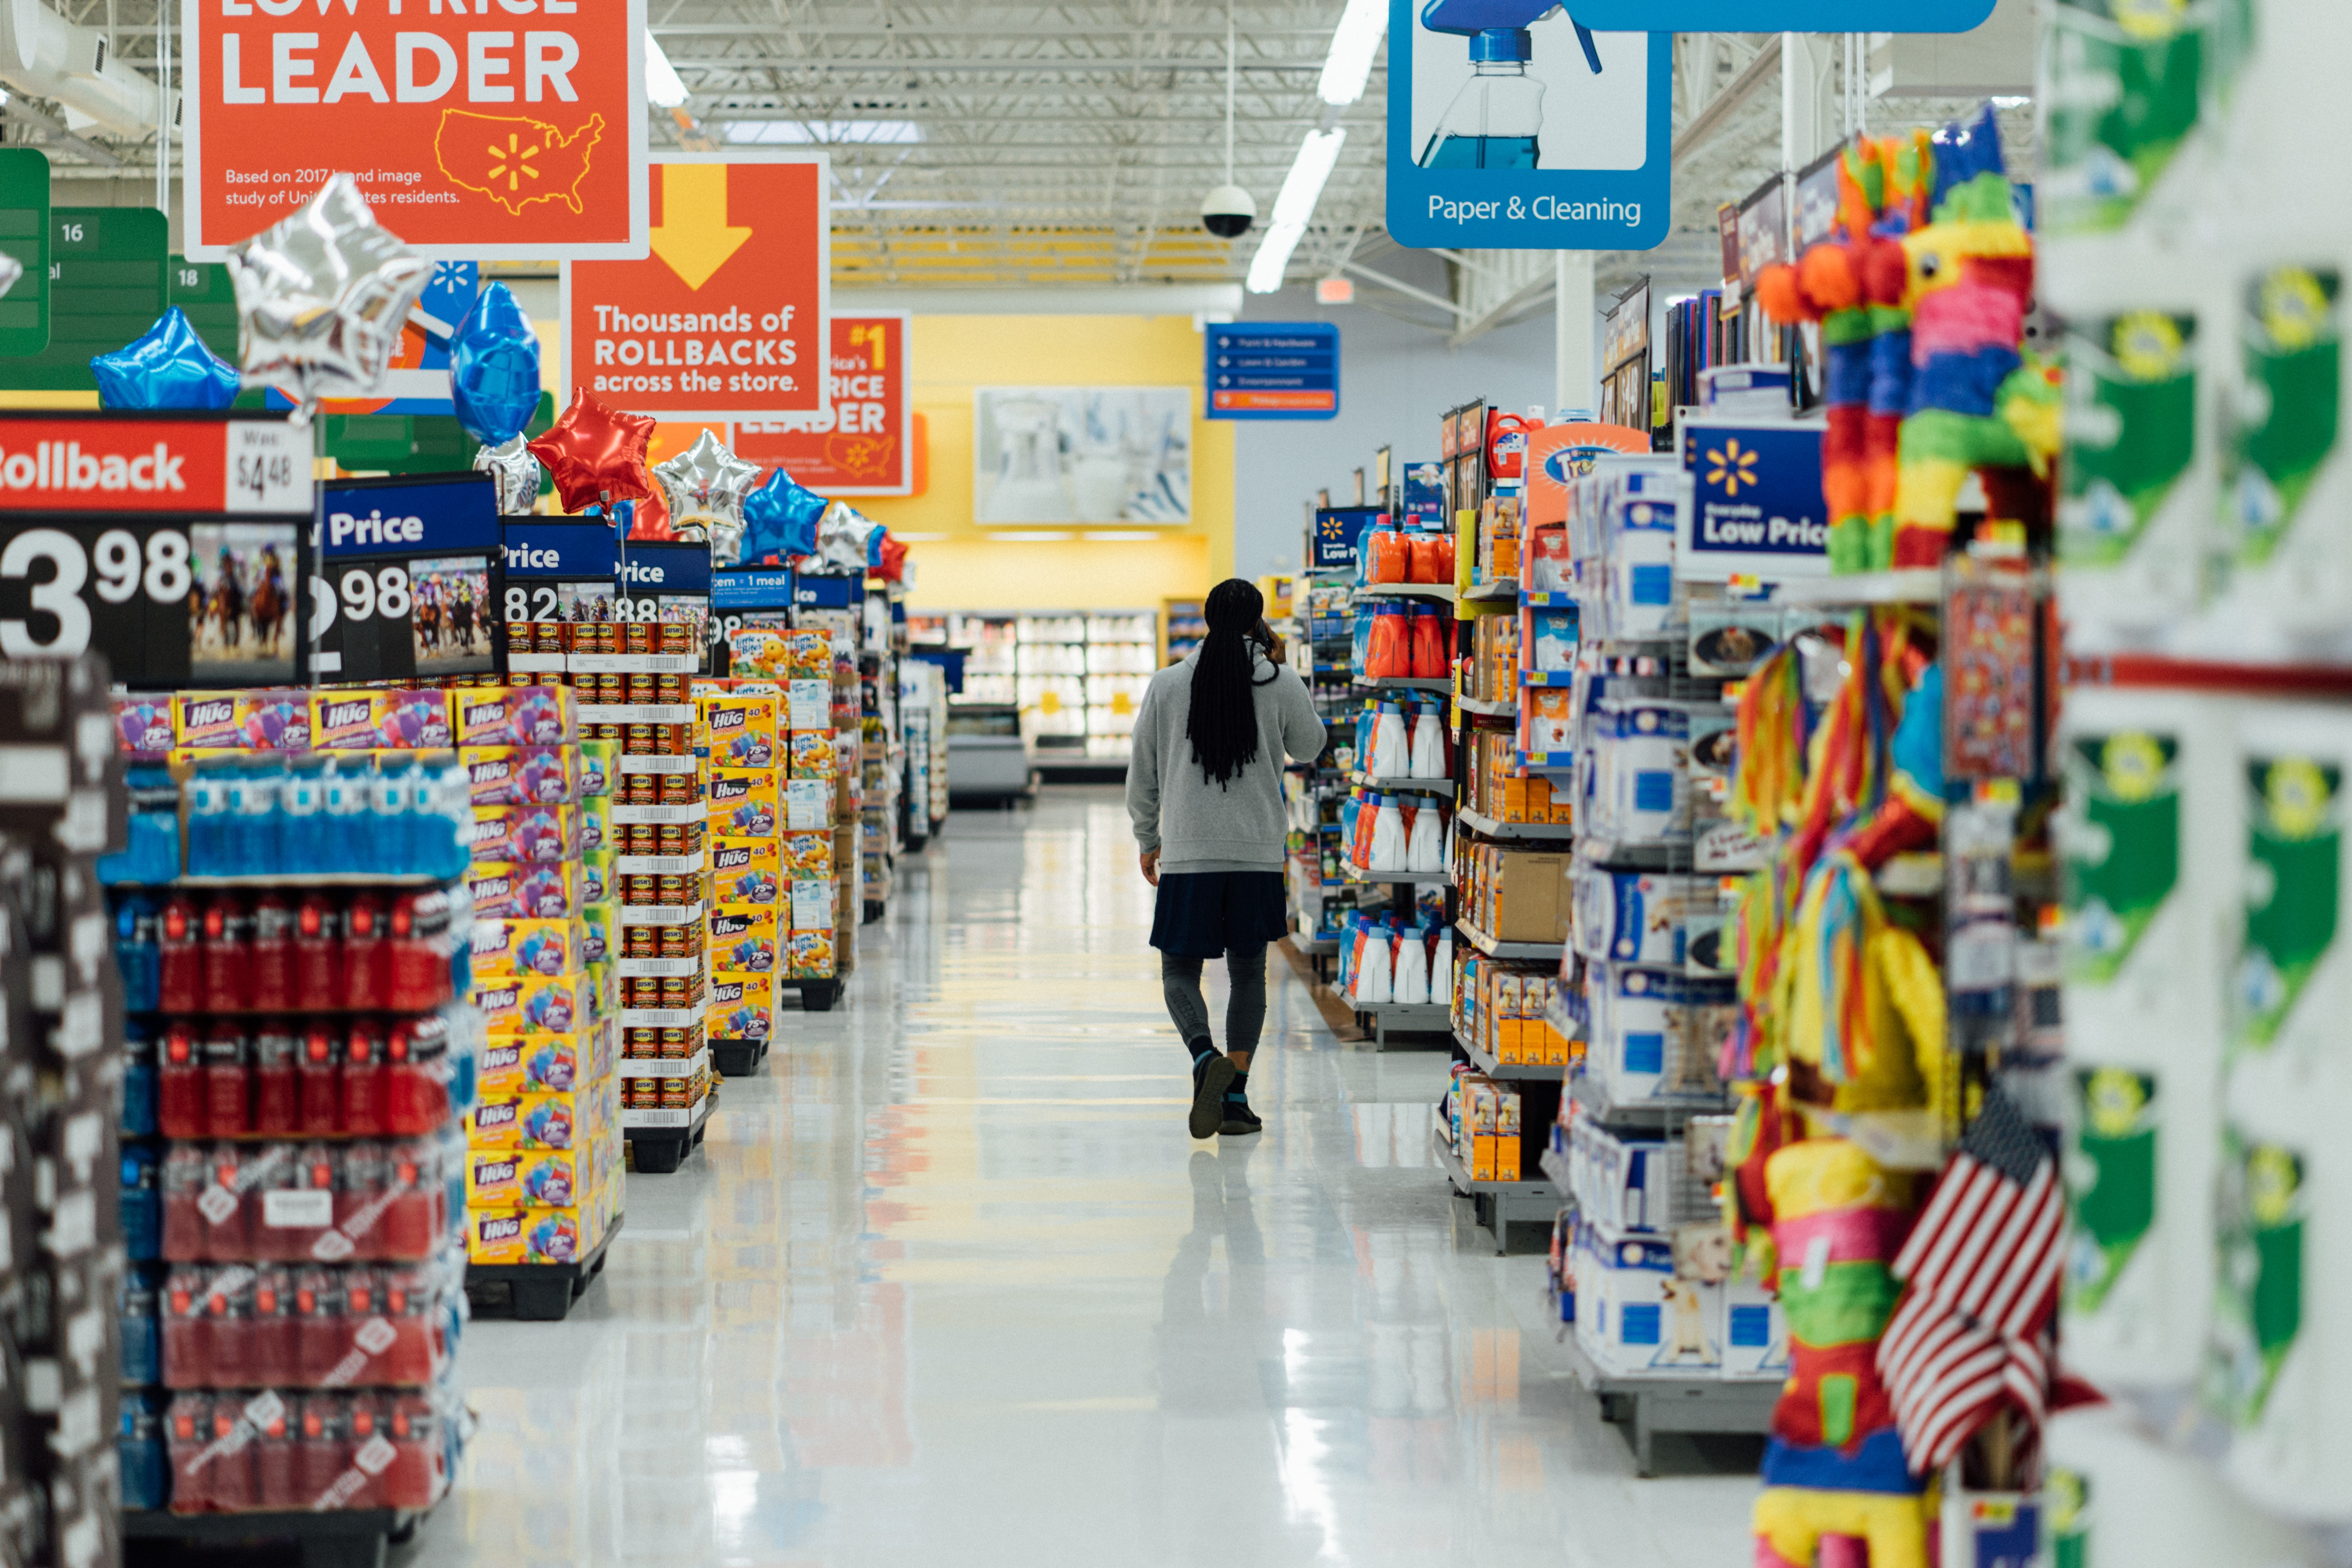
\includegraphics[width=0.4\textwidth]{gfx/04-store} 
\end{wrapfigure}
A research project always starts with someone who is curious about something observed. A grocery store clerk notices that cereal in red boxes seems to come through the checkout line more frequently than cereal in blue boxes and wonders why. An economist notices that during certain times of the year the motels seem to be full when other times they are not and wonders what causes that pattern. A driver on a delivery service wonders if there is a more efficient route for the daily deliveries.\blfootnote{Photo by Hanson Lu on Unsplash}

Researchers typically ``start where they are,'' an idea eloquently described by Kristin Esterberg\cite{esterberg2002qualitative}, who stated, ``Instead of thinking of yourself as a neutral, disinterested observer, think about the connections that you bring to what you plan to study.'' Whether it was thinking about a question they had pondered for some time, identifying a question about their own interests and hobbies, or taking a look at patterns in their everyday life, every researcher identifies a research question that was interesting and then collect and analyze data that helped answer that question. This chapter concerns creating a worthwhile question and planning a research project. Later chapters are devoted to collecting and analyzing data to answer a question.

Once researchers become curious about some topic of interest they must determine how they feel about the topic. An honest introspection is in order as they ask themselves what they may already believe about the topic and whether they believe that their perspective is the only valid one. If they determine that they have a preconceived notion that they think is the wisest perspective then that could be a problem. Researchers must also consider how they would react if their research proves them wrong about some believe. If they would be comfortable examining, and perhaps changing, what may be cherished notions based on their research then that is one thing, but if they would deny the research, hide the outcomes, or even change the data, then that would be a different problem altogether. Of course, just because a researcher feels strongly about a topic does not mean that it should be avoided; sometimes, the best topics to research are those about which someone feels strongly. 

Researchers who are prepared to accept all findings, even those that may be unflattering or challenging, may want to intentionally study a topic that evokes strong feelings. Sociology professor Kathleen Blee\cite{blee2005racial} has taken this route in her research. She studies hate movement participants and the people whose racist ideologies she does not share. Blee's research is successful because she was willing to report her findings and observations honestly, even those with which she may have personally taken strong issue.

One final step at this first stage is for researchers to think about what they already know about the topic of interest. There are many sources of knowledge, some are more prone to creating bias than others. For example, researchers may know of a topic from family history, a television program, or through casual conversations with friends. These could all introduce bias in the researcher's mind and it is important that researchers think about how they know what they know to help identify and correct biases that they may bring to the research project.

The purpose of this chapter is to outline a process that can be used to design a research project. To be sure, this is not the only possible way to design research, in fact, it may not even be the best way for a given research project, but it would work as a starting point for many research investigations.

\section{First Considerations}

Before starting the research design process, it would be helpful for the researcher to consider certain philosophical aspects of the project. While a failure to consider these items would not doom a research project, making these decisions early on may help to avoid messy re-starts. 

\subsection{Exploration, Description, Explanation}

Three general types of research are \gls{exploratoryresearch}, \gls{descriptiveresearch}, and \gls{explanatoryresearch}. Researchers conducting exploratory research are typically at the early stages of examining a topic. Exploratory research is often designed to determine the feasibility a more extensive study. Descriptive research describes or defines a particular phenomenon. As an example, an economist publishing the gasoline prices in various parts of a city is conducting descriptive research. Finally, research that answers ``why'' questions is referred to as explanatory research. In this case, the researcher is trying to identify the causes and effects of an observed phenomenon.

Although research can be exploratory, descriptive, or explanatory, most business research tends to be either descriptive or explanatory. Economists frequently produce research reports that describe the state of the economy without necessarily proposing some experiment to test that description. On the other hand, business and marketing research is frequently explanatory and is designed to develop concepts and theories that explain some observed phenomenon.

\subsection{Is The Topic Empirical?}

An empirical topic is one that can be investigated by observation or experience rather than one that concerns only opinions or theories. As an example, if a researcher investigated the cost of health care in order to answer the question, ``What is the best way to fund health care?'' that would not make an appropriate empirical study since the definition of ``best way'' is nebulous. The question, though, could be answered if it were re-framed a bit to simply how health care was funded then that would be a topic that could be measured and reported.

As a second example, in 2005 the Christian group \textit{Focus on the Family} denounced Spongebob Squarepants because they believe that he is a pro-gay activist as reported by David Kirkpatrick\cite{kirkpatrick2005conservatives}. Could a researcher determine if Spongebob is immoral? Of course not; this is an ethical question, not empirical. A researcher could gather facts about people's opinions concerning Spongebob and even interview the creators of the program to see what they intended, but answering the question of morality belongs to the world of ethicists or theologians, not business researchers.

\subsection{The Research Question}

Once a researcher finds a topic that is empirical then the next step is to write the research question. Following are the qualities of a good research question.

\begin{enumerate}
	\item Question. It may be rather obvious, but it must be written in the form of a question. To say that the research question is ``child-free adults'' or ``movies'' would not be a question. 
	\item Focused. A research question must be focused on one topic of interest and not something that is trying to explore many areas and hope that one of them ``sticks.''
	\item Open-ended. A research question should not be answered with a simple yes or no. For example, if a researcher asks, ``Does location influence the price of a real estate sale'' then there is nothing left to say once the ``yes'' or ``no'' answer is determined. Rather, a question like ``How does location influence the price of a real estate sale'' would be much better.
	\item Several answers. A good research question should have more than one plausible answer. If the question only has one possible answer then there is really nothing to research.
\end{enumerate}

\subsection{Hypotheses}

The purpose of \gls{positivist} research\footnote{Researchers engaged in interpretive projects may not start with a hypothesis, but one would likely be developed as the research project proceeded.} is to test a theory and in order to do that a researcher must create a \gls{hypothesis} that is derived from the theory. A hypothesis is a statement, sometimes causal, describing a researcher's expectation regarding the anticipated result of the investigation. Often, hypotheses are written to describe the expected relationship between two \glspl{variable}. Hypotheses are typically based on a theory and describe how an independent variable is expected to affect some dependent variable. If the theory accurately reflects the phenomenon it is designed to explain then the researcher's hypotheses should be verified.

As an example, Social Exchange Theory postulates, among other things, that positive outcomes from social exchanges over time increases trust and commitment\cite{lambe2001social}. A researcher may hypothesize that brand loyalty increases due to positive outcomes from social exchanges and then design some sort of investigation to test that hypothesis.

Sometimes, researchers hypothesize that a relationship will take a specific direction so an increase in one variable might lead to an increase in another; the variables are correlated. For example, a researcher may study the relationship between age and consumers' preference for sustainable products. The hypothesis may be something like ``younger consumers tend to prefer sustainable products more than older consumers.'' The research would be designed to determine if there is a difference in product preference by age. 

Note that researchers never say that they have proven a hypotheses. A statement that bold implies that a relationship has been shown to exist with absolute certainty and that there is no chance that there are conditions under which the hypothesis fail. Instead, researchers tend to say that their hypotheses have been supported (or not). This more cautious way of discussing findings allows for the possibility that new evidence or new ways of examining a relationship will be discovered. Researchers may also discuss a ``null hypothesis,'' one that predicts no relationship between the variables being studied. If a researcher ``rejects the null hypothesis,'' then it means that the variables in question are somehow related to one another.

\subsection{Feasibility}

In Chapter \ref{03:ethics}, \nameref{03:ethics}, ethical considerations were discussed that may make some research projects unfeasible. Certainly, no researcher is going to design an experiment where a business enterprise would intentionally injure children in order to test some theory. There are, though, a few practical matters related to the feasibility of a study that researchers should consider before beginning a project. 

Gaining unfettered access to a population could be problematic. For example, a project that included exploring the day-to-day experiences of maximum security prisoners may not be feasible due to the limited access a researcher would have to that population. On a more practical level, even research about something as common as children's behavior concerning snacks can raise interesting research issues. For example, Marshall, O'Donohoe, and Kline\cite{marshall2007families} conducted a study where they interviewed $ 8-11 $ year-old children to explore their exposure to food advertising and subsequent snack preference. While it is, generally, no trouble to find children that age to interview, there are questions about how honest children are with adults in a formal interview setting. While children do not necessarily intentionally lie, their responses to interview questions are almost certainly influenced by the fact than an adult is asking. What children say to each other during play would, no doubt, be far different from what they tell an adult during an interview. It may be impossible for an adult to ever truly enter the world of a child to observe what they say and do. 

Another consideration would be the limits imposed by time. Suppose a researcher wants to investigate how shopping habits change in a community that is becoming gentrified. Sullivan\cite{sullivan2014food} conducted surveys to determine the demographic characteristics of shoppers who were purchasing organic food in gentrified neighborhood. Bridge and Dowling\cite{bridge2001microgeographies} considered gentrification from the perspective of the retail landscape in several gentrified neighborhoods. However, to understand the \textit{change} that gentrification brings a researcher may need to observe a neighborhood for many years and record the demographics of the families who are shopping, interview them to find out what they are thinking and experiencing, and even analyze what they purchase. Unfortunately, researchers rarely have decades to devote to a single project so this type of longitudinal study becomes unfeasible.

The funding available for a study is also potentially limiting. Medical research often requires the use of very expensive equipment, like particle accelerators (more than \$100 million), Computerized Axial Tomography (CAT) Scanners (up to \$2.5 million), and Magnetic Resonance Imaging machines(about \$1 million). Even surveys that use equipment no more expensive than paper and pencil require researchers to spend time interviewing shoppers. If the research project involves a team of survey-takers fanning out over a wide geographic ares over several weeks then the personnel cost could easily top \$100 thousand. Even something as inexpensive as offering a participant a cup of coffee during an interview has a small, but quantifiable, cost that must be met.

In sum, the feasibility of a research project must be considered when deciding how to complete the project, or even if the project can be completed at all.

\subsection{Idiographic or Nomothetic?}

In general terms, research can be described as \gls{idiographic} or \gls{nomothetic}, as described by Joseph Ponterotto\cite{ponterotto2005qualitative}. These terms derive from Kantian philosophy and are frequently found in research reports, especially in psychology and sociology. However, understanding these concepts is beneficial in the planning stage for research in any field.

\begin{itemize}
	\item Idiographic. This term comes from the Greek \textit{idios}, which refers to an individual. Idiographic research concerns a single case or entity with no expectation that the research would be applicable to a wider application. Idiographic research sacrifices breadth of application for deeper, richer understanding of a single case. Many case studies are idiographic in the sense that only a single individual or location is studied and applicability beyond that case is not reasonable. Much of the small business research being done is idiographic in nature.
	\item Nomothetic. This term comes from the Greek \textit{nomos}, which refers to the traditional social norm. The goal of nomothetic research is to predict or explain general phenomena found in a population rather than a single case. Nomothetic research sacrifices understanding of single cases for a broader application across an entire industry. Much economic research is nomothetic in nature since it attempts to explain broad trends in an entire population. For example, an economist may predict that the economy will begin to improve but that does not guarantee that a specific business will benefit.
\end{itemize}

\subsection{Applied or Basic?}

The contribution that researchers hope to make to the body of knowledge depends on whether they are conducting \gls{appliedresearch} or \gls{basicresearch}. Applied research can be immediately applied to a specific case. Applied research would help a small business owner made changes in advertising that would improve the number of customers entering the store. Basic research, on the other hand, is designed to create, or validate, theories and would be useful to a legislator considering some change in the business laws of a state.

\subsection{Units of Analysis}

Another point to consider when designing a research project, and which might differ slightly in \gls{qualitativeresearch} and \gls{quantitativeresearch}, has to do with units of observation and units of analysis. These two items concern what the researcher observes in the course of data collection and what can later be said about those observations. A unit of observation is the item (or items) that are actually observed, measured, or collected in the course of of the research study. A unit of analysis is the entity that is reported at the end of the study, or the ``main focus'' of the study. In a given study, the unit of observation might be the same as the unit of analysis, but that is not always the case. What is required, however, is for researchers to be clear about how they define their units of observation and analysis, both to themselves and to their audiences.

As an example, one common unit of analysis is an individual. A research project designed to look at the shopping habits of people would use the individual as the unit of analysis. Market basket research, where the content of a shopper's basket is analyzed, uses the individual as the unit of analysis. A researcher may be interested in how some particular product makes a person feel or what thought process someone used to select a given product. One example of an individual unit of analysis can be found in investigating the role of social marketing on sales and services, as investigated by Alan Bright\cite{bright2000role} and Philip Kotler\cite{kotler1989social}.

A second common unit of analysis is groups. Groups, of course, vary in size and almost no group is too small or too large to be of interest to researchers. Families, friendship groups, and civic clubs (like \textit{Rotary}) are a few common groups examined by researchers. As examples, researchers might study how norms of workplace behavior vary across professions or how children's sporting clubs are organized. A rich and vast body of research has been done on small businesses and this would be using a group unit of analysis\cite{yusuf1995critical}\cite{huck1991competencies}.

Organizations are yet another potential unit of analysis that researchers might wish to say something about. Organizations are large groups where the members are not necessarily as homogeneous as in a small group and includes entities like corporations, colleges and universities, and even night clubs.

As examples, researchers might study the economic impact of globalization or how unions influence the behavior of industry leadership, as researched by Diana Hechavarria\cite{hechavarria2009cultural} and Randall Schuler\cite{schuler1998understanding}.

Social phenomena are a potential unit of analysis. Social phenomena such as voting and even cell phone app use or misuse would be phenomena that could be researched.

Finally, researchers examine policies and principles in businesses and those are typically contained in documents. In this case, then, the unit of observation would be a document while the unit of analysis is the business. This is also a good example of where the unit of observation and unit of analysis are different.

In sum, there are many potential units of analysis that a sociologist might examine, but some of the most common include:

\begin{enumerate}
	\item Individuals
	\item Groups
	\item Organizations
	\item Social phenomena
	\item Policies and principles
\end{enumerate}

There are also many topics that could be studied from more than one level of analysis, though that would become a more complex study. As an example, Kuruvilla and Ranganathan researched the way micro and macro human resource policies influenced economic development strategy in India\cite{kuruvilla2008economic}.

\section{The Research Process}\label{04:process}

Broadly speaking, research methods can be grouped into two broad categories: \gls{positivism} and \gls{interpretivism}. 
% TODO Can you come up with a graphic to compare positivism and interpretivism?

\subsection{Positivism}

\begin{itemize}
	\item Goal: theory testing
	\item Methods: laboratory experiments and surveys
	\item Approach: deductive, starts from theory and generates empirical data to test the theory
	\item Data: quantitative in nature: numeric 
	\item Analysis: statistical
\end{itemize}

\subsection{Interpretivism}

\begin{itemize}
	\item Goal: theory building
	\item Methods: action research and ethnography
	\item Approach: inductive, starts from observations and generates theory
	\item Data: qualitative in nature: textural
	\item Analysis: coding
\end{itemize}

\subsection{Iterative Design}

At its core, all scientific research is an iterative process of observation, rationalization, and validation. In the observation phase, researchers observe a natural or social phenomenon, event, or behavior of interest. In the rationalization phase, they try to make sense of the observed phenomenon, event, or behavior by logically connecting the different pieces of the puzzle; which, in some cases, may lead to the construction of a theory. Finally, in the validation phase, those theories are scientifically tested using a process of data collection and analysis and that often leads to a modification of the initial theory. However, research designs vary based on whether the researcher starts at observation and attempts to generate a theory (interpretive research) or starts at a theory and attempts to validate it with observations (positivist research).

Most traditional research tends to be positivist in nature. Figure \ref{fig04.01} provides a schematic view of such a research project. This figure depicts a series of activities to be performed, categorized into three phases: exploration, research design, and research execution. \marginpar{This generalized design does not fit all research and it should be modified to fit the needs of a specific project.}

\begin{figure}[H]
	\centering
	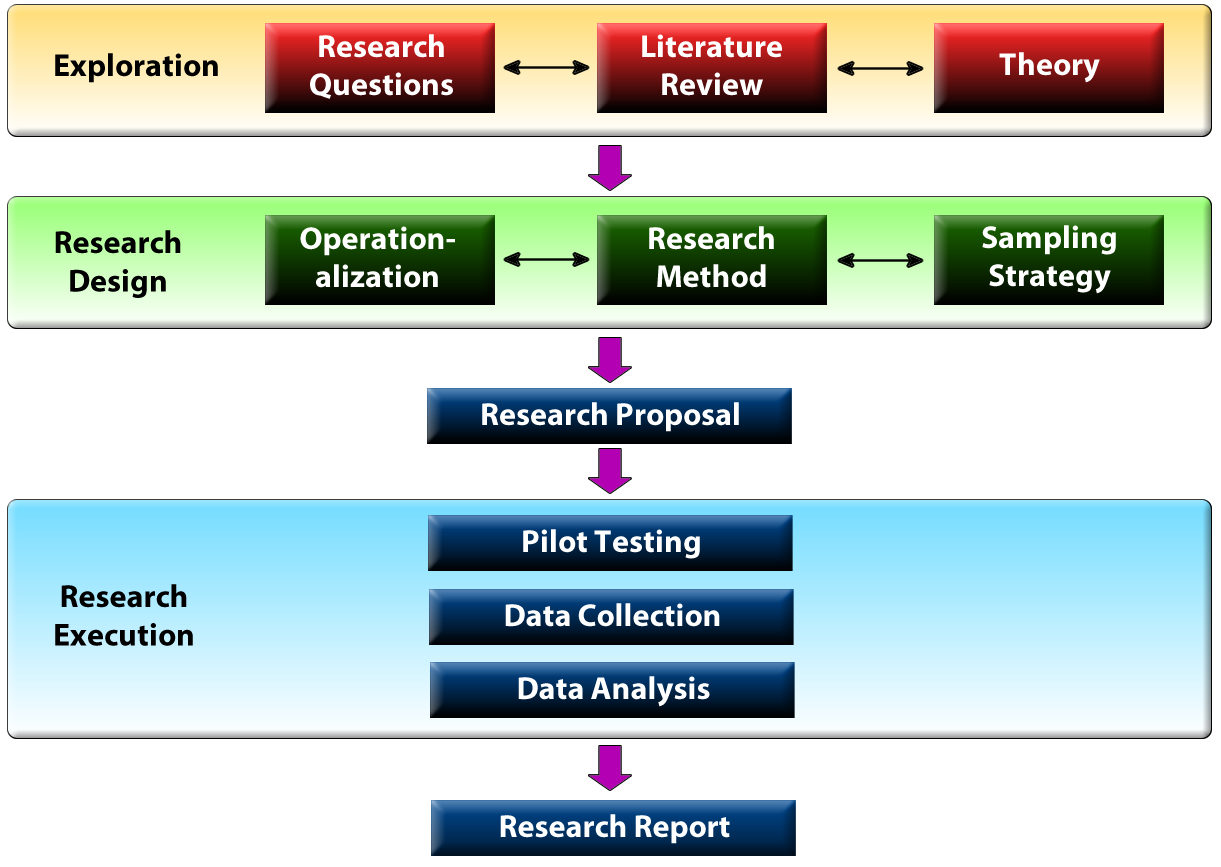
\includegraphics[width=\linewidth]{gfx/04-01}
	\caption{Positivist Research Process}
	\label{fig04.01}
\end{figure}

\begin{enumerate}
	\item \textbf{Exploration}. The first phase is exploration, which includes exploring and selecting research questions for further investigation, examining the published literature in the area of inquiry to understand the current state of knowledge in that area, and identifying theories that may help answer the research questions of interest. The diagram makes it clear that these three steps often run concurrently and researchers typically shift back-and-forth between them as needed. For example, a literature review is designed to uncover pertinent theories but finding those theories may lead to further literature review.

\begin{itemize}
	\item The first step in the exploration phase is identifying one or more research questions that deal with a specific behavior, event, or phenomena of interest. Examples include what factors motivate consumers to purchase goods and services online without knowing the vendors of these goods or services, how can high school students become more creative, and why do some people commit terrorist acts. More 	interesting research questions are those that appeal to a broader population (e.g., ``how can firms innovate'' is a more interesting research question than ``how can Chinese firms innovate in the service-sector''), address real and complex problems (in contrast to hypothetical problems), and where the answers are not obvious. Narrowly focused research questions (often with only a \textit{yes/no} answer) tend to be less useful and interesting, and generally lead to unpublishable research findings.

	\item The next step is to conduct a literature review of the domain of interest. The purpose of a literature review is three-fold: 1) to survey the current state of knowledge in the area of inquiry, 2) to identify key authors, articles, theories, and findings in that area, and 3) to identify gaps in the knowledge that a research project may be able to fill. \marginpar{Literature review is commonly done using searches in online databases.} Once a shortlist of relevant articles is generated from a search the researcher must then manually browse through each article, or at least its abstract, to determine the suitability of that article for a detailed review. Literature reviews should be reasonably complete and not restricted to only a few journals, a few years, or a specific methodology. Reviewed articles may be summarized in the form of tables and can be further structured using organizing frameworks such as a concept matrix. A well-conducted literature review should indicate whether the initial research questions have already been addressed in the literature (which would obviate the	need to study them again), whether there are newer or more interesting research questions available, and whether the original research questions should be modified or changed in light of findings of the literature review. The review can also provide some intuitions or potential answers to the questions of interest and/or help identify theories that have previously been	used to address similar questions. Reading scholarly literature is different from reading a textbook or novel. Scholarly literature is typically divided into predictable sections. One of the easiest to find is the abstract, which is a short paragraph at the beginning of an article that summarizes the research question, methods used to answer the question, and key findings. The abstract often shows whether the article is relevant to the research project. Most scholarly articles contain these sections: introduction, literature review, methodology, findings, and discussion. After the abstract, reading the discussion section is usually the next most productive. Finally, the methodology section may include important clues about a productive way to approach a research project.
	
	\item Since positivist research involves theory-testing, the third step is to	identify one or more \glspl{theory} that can help address the desired research questions. While the literature review may uncover a wide range of concepts or \glspl{construct} potentially related to the phenomenon of interest, a theory will help identify which of these constructs is logically relevant to the target phenomenon and how. Failing to identify related theories may result in measuring a wide range of less relevant, or even irrelevant constructs, while also minimizing the chances of obtaining results that are meaningful. In positivist research, theories can be used as the logical basis for postulating \glspl{hypothesis} needed in a later step. Obviously, not all theories are well-suited for studying all phenomena. Theories must be carefully selected based on their fit with the target problem and the extent to which their assumptions are consistent with that of the target problem.
	
\end{itemize}

\item \textbf{Research Design}. The next phase in the research process is research design. This process creates a blueprint of research activities that will satisfactorily answer the questions identified in the exploration phase. This includes selecting a research method, operationalizing constructs of interest, and devising an appropriate sampling strategy.

\begin{itemize}
	\item \Gls{operationalization} is the process of designing precise measures for abstract theoretical constructs. This is a major problem in business and marketing research given that many of the constructs, like ``average family'' and ``organizational culture,'' are hard to define and challenging to measure. Operationalization starts with specifying an ``operational definition'' (or ``conceptualization'') of the constructs of interest. Next, the researcher searches the literature to see if there are existing measures that can be modified to measure the constructs of interest. If such measures are not available or if they reflect a different conceptualization than that intended by the researcher then new instruments may have to be designed. This can easily be a long and laborious process, with multiple rounds of pretests and modifications before the newly-designed instrument can be accepted as ``scientifically valid.''
	
	\item Simultaneously with operationalization, the researcher must also decide what research method to employ for collecting data that will address the research question. Informing this stage of the process are the answers to philosophical questions like whether the research be exploratory, descriptive, or explanatory; will the approach be interpretive or positivist; is the goal to have some direct application or contribute more generally to the field; and what unit of analysis and observation will be used. Research methods may include experimentation, surveys, case studies, and others, or combinations of several methods in order to triangulate an answer. The selected method must then be further refined, for example, surveys could be administered by mail, telephone, web, or a combination.
	
	\item Researchers must also carefully choose the target population and a sampling strategy for data collection. While selecting a sample, care should be taken to avoid a biased sample that may generate biased observations. Sampling is covered in depth in a later chapter.
	
\end{itemize}

\item \textbf{Proposal}. At this stage, it is often a good idea to write a research proposal detailing all of the decisions made in the preceding stages of the research process and the rationale behind each decision. This multi-part proposal should address the research questions being studied and why, the current state of knowledge, theories and hypotheses to be tested, how the constructs will be measured, the research method to be employed and why, and sampling strategy. Funding agencies typically require a detailed proposal in order for them to select which to fund. Even if funding is not sought for a research project, a proposal may serve as a useful vehicle for seeking feedback from other researchers and identifying potential problems with the research project before starting data collection. This initial feedback is invaluable because it is often too late to correct critical problems after data is collected in a research study.

\item \textbf{Research Execution}. Having decided who to study (subjects), what to measure (concepts), and how to collect data (research method), the researcher is now ready to proceed to the research execution phase. This includes pilot testing the measurement instruments, data collection, and data analysis.

\begin{itemize}
	\item Pilot testing is an often overlooked but extremely important part of the research process. It helps detect potential problems in the research design and instrumentation (e.g., whether survey questions are intelligible to the targeted sample), and to ensure that the measurement instruments used in the study are reliable and valid measures of the constructs of interest. The pilot sample is usually a small subset of the target population. After a successful pilot testing, the researcher may then proceed with data collection using the sampled population.
	
	\item Next comes the actual collection of data. At this phase of the investigation the researcher would conduct surveys, visit field sites, interview subjects, read corporate documents, or generate whatever other data is specified by the plan.
	
	\item Following data collection, the data are analyzed and interpreted for the purpose of drawing conclusions regarding the research questions. Depending on the type of data collected (quantitative or qualitative), data analysis may be quantitative (e.g., employ statistical techniques such as regression or structural equation modeling) or qualitative (e.g., coding or content analysis).
		
\end{itemize}

\item \textbf{Research Report}. The final phase of research involves preparing the final research report documenting the entire research process and its findings in the form of a research paper, dissertation, or monograph. The report should outline in detail all the choices made during the research process (e.g., theory used, constructs selected, measures used, research methods, sampling, etc.) and why, as well as the outcomes of each phase of the research process. The research process must be described in sufficient detail so as to allow other researchers to replicate the study, test the findings, or assess whether the inferences derived are scientifically acceptable. Research is of no value unless the process and outcomes are documented for future generations and such documentation is essential for the progress of science.
	
\end{enumerate}

\section{Mixed Methods}

Up to this point, the research design has been treated as if it is an either/or proposition. Either a research project is positivist and numeric data are gathered or it is interpretative and textural data are gathered. In truth, researchers do not necessarily have to choose one approach over another. In fact, some of the most highly regarded business and marketing investigations combine approaches in an effort to gain the most complete understanding of their topic possible. Using a combination of multiple and different research strategies is called mixed methods because the goal is to focus on ``truth'' from several different approaches.

Imagine that a researcher were interested in finding out how college students used electronic devices on campus. Instead of just conducting one type of research, maybe a survey, two research techniques could be used, a survey and individual interviews. Finally, add to the project a content analysis of campus policies and observations of students in their natural environments\footnote{For information about using a mixed method type of research design, see John Brewer\cite{brewer1989multimethod} and Charles Teddlie\cite{teddlie2006general}.}. Researchers would end up with a comprehensive understanding of how students use electronic devices on campus. The drawback, of course, is that a mixed method project requires a larger number of resources, time, and expertise to complete. Also, along with gaining the benefit of the strengths of each type of research is the potential of the combined weaknesses becoming a problem.

\section{Common Research Mistakes}

The research process is fraught with problems and pitfalls and novice researchers often find after investing substantial amounts of time and effort into a research project that their research questions were not sufficiently answered, or that the findings were not interesting enough, or that the research was not of ``acceptable'' scientific quality. Such problems typically result in research papers being rejected by journals.

\begin{itemize}
	\item Insufficiently motivated questions. Often times, researchers choose ``pet'' problems that are interesting to the individual but not to the scientific community at large, i.e., it does not generate new knowledge or insight about the phenomenon being investigated. Because the research process involves a significant investment of time and effort on the researcher's part, the researcher must be certain (and be able to convince others) that the research questions they seek to answer in fact deal with real problems (and not hypothetical problems) that affect a substantial portion of a population and has not been adequately addressed in prior research.

	\item Pursuing research fads. Another common mistake is pursuing ``popular'' topics with limited shelf life. A typical example is studying technologies or practices that are popular today but may be obsolete in just a few years (or months). Because research takes several years to complete and publish, it is possible that popular interest in these fads may die down by the time the research is completed and submitted for publication. A better strategy may be to study ``timeless'' topics that have persisted through the years.

	\item Unresearchable problems. Some research problems may not be answered adequately based on observed evidence alone or currently accepted methods and procedures. Such problems are best avoided. However, some unresearchable, ambiguously defined problems may be modified or fine tuned into well-defined and useful researchable problems.

	\item Favored research methods. Many researchers have a tendency to recast a research problem so that it is amenable to their favorite research method (\eg, survey research). This is an unfortunate trend. Research methods should be chosen to best fit a research problem, and not the other way around.

	\item Blind data mining. Some researchers have the tendency to collect data first (using instruments that are already available), and then figure out what to do with it. In reality, data collection is only one step in the long process of planning, designing, and executing research. In fact, a series of other activities are needed in a research process prior to data collection. If researchers jump into data collection without such elaborate planning, the data collected will likely be irrelevant, imperfect, or useless, and their data collection efforts may be entirely wasted. An abundance of data cannot make up for deficits in research planning and design, and, particularly, for the lack of interesting research questions.

	\item Ecological fallacy. This occurs when claims about one lower-level unit of analysis are made based on data from some higher-level unit of analysis. In many cases, this occurs when claims are made about individuals, but only group-level data have been gathered. 

	\item Reductionism. This occurs when claims about some higher-level unit of analysis are made based on data from some lower-level unit of analysis. As an example, claims about groups are made based on individual-level data.

\end{itemize}

\section{Research Designs}

As noted on page \pageref{04:process}, research designs can be classified into two categories, \gls{positivism} and \gls{interpretivism}, depending upon the researcher's background, temperament, and research goal. Positivist designs are meant for theory testing while interpretive designs are meant for theory building. Popular examples of positivist designs include experimental (both laboratory and field), surveys, secondary data analysis, and case research while interpretive designs include case research, phenomenology, and ethnography. Note that case research can be used for both theory building and theory testing, though not at the same time. Some techniques, such as focus groups, are best suited for exploratory research, others such as ethnography are best for descriptive research, and still others such as laboratory experiments are ideal for explanatory research.

\subsection{Experimental}

Experimental studies are those that are intended to test cause-effect relationships (hypotheses) in a tightly controlled setting by separating the cause from the effect in time, administering the cause to one group of subjects (the ``treatment group'') but not to another group (``control group''), and observing how the mean effects vary between subjects in these two groups. For instance, if a laboratory experiment is designed to test the efficacy of a new drug in treating a certain ailment then a random sample of people afflicted with that ailment is found and they are randomly assigned to one of two groups (treatment and control). The drug is administered to subjects in the treatment group while a placebo is given to the control group. Finally, the two groups are monitored over a period of time to see if the treatment group has a better response than the control group. More complex designs may include multiple treatment groups, such as low versus high dosage of the drug, and multiple treatments, such as combining drug administration with dietary interventions. 

In an experimental design the subjects are randomly assigned to a group. It is ideal if the researcher knows whether individuals are in the treatment or control groups but the scientists actually administering the treatment protocol are not sure if a specific subject is receiving the drug under test or a placebo. This type of design is called a ``double-blind'' study since neither the subject nor the person administering the treatment are sure if they are in the treatment group.

If random assignment is not possible for some reason then the research design becomes ``quasi-experimental.''

Experiments can be conducted in a laboratory setting such as at a university (laboratory experiments) or in a field settings such as in an organization where the phenomenon of interest is actually occurring (field experiments). Laboratory experiments allow the researcher to isolate the variables of interest and control for extraneous variables which may not be possible in field experiments. Hence, inferences drawn from laboratory experiments tend to be stronger in internal \gls{validity}\footnote{Validity is more thoroughly defined in Chapter \ref{ch05:measuring}, page \pageref{ch05:measuring}}, but those from field experiments tend to be stronger in external validity. 

Experimental data are analyzed using quantitative statistical techniques. The primary strength of the experimental design is its strong internal validity due to its ability to isolate, control, and intensively examine a small number of variables, while its primary weakness is limited external generalizability since real life is often more complex (i.e., involve more extraneous variables) than contrived lab settings. Furthermore, if the research does not identify relevant extraneous variables and control for those variables it may decrease internal validity and lead to spurious correlations.

\subsection{Surveys}

Field surveys are non-experimental designs that do not control for or manipulate independent variables or treatments but measure these variables and test their effects using statistical methods. Field surveys capture snapshots of practices, beliefs, or situations from a random sample of subjects in field settings through a survey questionnaire or, less frequently, through a structured interview. In cross-sectional field surveys, independent and dependent variables are measured at the same point in time (e.g., using a single questionnaire), while in longitudinal field surveys, dependent variables are measured at a later point in time than the independent variables. The strengths of field surveys are their external validity (since data is collected in field settings), their ability to capture and control for a large number of variables, and their ability to study a problem from multiple perspectives or using multiple theories. However, because of their non-temporal nature, internal validity (cause-effect relationships) is problematic. Surveys may also be subject to respondent biases (e.g., subjects may provide a ``socially desirable'' response rather than their true response) which further decreases internal validity.

\subsection{Secondary Data Analysis}

Secondary data analysis is analysis of data that has previously been collected and tabulated by other sources. Data sources may include government agencies (e.g. employment statistics from the U.S. Bureau of Labor Statistics), other researchers (e.g. dissertations), or publicly available third-party data (financial data from stock markets). This is in contrast to most other research designs where collecting primary data for research is part of the researcher's job. Secondary data analysis may be an effective means of research where primary data collection is too costly or unfeasible and secondary data is available at a level of analysis suitable for answering the research questions. The limitations of this design are that the data may not have been collected in a systematic or scientific manner and hence unsuitable for scientific research. Also, since the data were collected for a presumably different purpose, they may not adequately address the research questions of interest to the researcher. Finally, interval validity is problematic if the temporal precedence between cause and effect is unclear.

\subsection{Case Research}

Case research\footnote{It is important to keep in mind that case research is not the same as a business class discussing a classic Harvard Case Study. Case research is the process of actually going to a site, gathering data, and analyzing that data.} is an in-depth investigation of a problem in one or more real-life settings (case sites) over an extended period of time. Data may be collected using a combination of interviews, personal observations, and internal or external documents. Case studies can be positivist in nature (for hypotheses testing) or interpretive (for theory building). The strength of this research method is its ability to discover a wide variety of social, cultural, and political factors potentially related to the phenomenon of interest that may not be known in advance. Analysis tends to be qualitative in nature, but heavily contextualized and nuanced. Weaknesses of case research include dependence on the observational and analytical ability of the researcher, lack of control which makes it difficult to establish causality, and inability to generalize findings from a single case site to other case sites. Generalizability can be improved by comparing the analysis from other case sites in a multiple case design.

\subsection{Focus Groups}

Focus group research is a type of research that involves bringing in a small group of subjects (typically six to ten people) to one location and having them discuss a phenomenon of interest for a period of about two hours. The discussion is moderated by a trained facilitator who sets the agenda and poses an initial set of questions for participants, then ensures that ideas and experiences of all participants are recorded, and then attempts to build an understanding of the problem based on participants' comments. Internal validity cannot be established due to lack of controls and the findings may not be generalized to other settings because of small sample size. Hence, focus groups are not generally used for explanatory or descriptive research but are suited for exploratory research projects.

\subsection{Action Research}

Action research assumes that complex social phenomena are best understood by introducing interventions, or ``actions,'' into those phenomena and then observing the effects of those actions. In this method, the researcher is usually a consultant or an organizational member embedded within a social context, such as an organization, who initiates an action, such as new organizational procedures or new technologies, in response to a real problem, such as declining profitability or operational bottlenecks. The researcher's choice of actions must be based on theory, which should explain why and how such actions may cause the desired change. The researcher then observes the results of that action, modifying it as necessary, while simultaneously learning from the action and generating theoretical insights about the target problem and interventions. The initial theory is validated by the extent to which the chosen action successfully solves the target problem. Simultaneous problem solving and insight generation is the central feature that distinguishes action research from all other research methods, and hence, action research is an excellent method for bridging research and practice. This method is also suited for studying unique social problems that cannot be replicated outside that context, but it is also subject to researcher bias and subjectivity, and the generalizability of findings is often restricted to the context where the study was conducted.

\subsection{Ethnography}

Ethnography is an interpretive research design inspired by anthropology that emphasizes the concept that a phenomenon must be studied within the context of its culture. The researcher is deeply immersed in a certain culture over an extended period of time (a few months to several years) and during that period engages, observes, and records the daily life of the studied culture. The ultimate goal is a theory about the evolution and behaviors in that culture. Data are collected primarily via observational techniques, formal and informal interaction with participants in that culture, and personal field notes, while data analysis involves ``sense-making.'' The advantages of this approach are its sensitiveness to the context, the rich and nuanced understanding it generates, and minimal respondent bias. However, this is also an extremely time and resource-intensive approach, and findings are specific to a given culture and less generalizable to other cultures.

\section{Selecting the Research Design}

Researchers tend to select designs that they are most comfortable with and feel most competent to handle; but, ideally, the choice should depend on the nature of the research phenomenon being studied. In the preliminary phases of research, when the research problem is unclear and the researcher wants to scope out the nature and extent of a certain research phenomenon, a focus group (for individual unit of analysis) or a case study (for organizational unit of analysis) is an ideal strategy for exploratory research. As the research project evolves, interpretive designs, such as case research or ethnography may be useful. If a literature review finds competing theories then positivist designs such as experimental, survey, or secondary data analysis are more appropriate.

Regardless of the specific research design chosen, the researcher should attempt to collect both quantitative and qualitative data using a combination of techniques such as questionnaires, interviews, observations, documents, or secondary data. For example, even in a highly structured survey questionnaire intended to collect quantitative data, the researcher may leave room for a few open-ended questions to collect qualitative data that may generate unexpected insights not otherwise available from the structured quantitative data alone. Likewise, while case research employ mostly face-to-face interviews to collect most qualitative data, the potential and value of collecting quantitative data using a concurrent survey should not be ignored. As an example, in a study of organizational decision-making processes, the case interviewer could record numeric quantities such as how many months it took to make certain organizational decisions, how many people were involved in that decision process, and how many alternatives were considered, and those data can provide valuable insights not otherwise available from interviewees' narrative responses. Irrespective of the specific research design employed, the goal of the researcher should be to collect as much and as diverse data as possible that can help generate the best possible insights into the phenomenon of interest.

\section{Summary}\label{ch05:summary}

Lorem ipsum dolor sit amet, consectetuer adipiscing elit. Aenean commodo ligula eget dolor. Aenean massa. Cum sociis natoque penatibus et


\ctparttext{Quantitative methods are based in the measurement of concepts and the statistical analysis of those measures. Quantitative methods include activities like sampling, surveys, and experimental research.}
\part{Quantitative Methods}
\cleardoublepage
%%*****************************************
\chapter{Defining and Measuring Concepts}\label{ch05:measuring}
%*****************************************
%TODO Status: Pre-draft

\section{Measurement}

\begin{wrapfigure}{r}{0.2\textwidth}
	\label{05:fig01} 
	\centering
	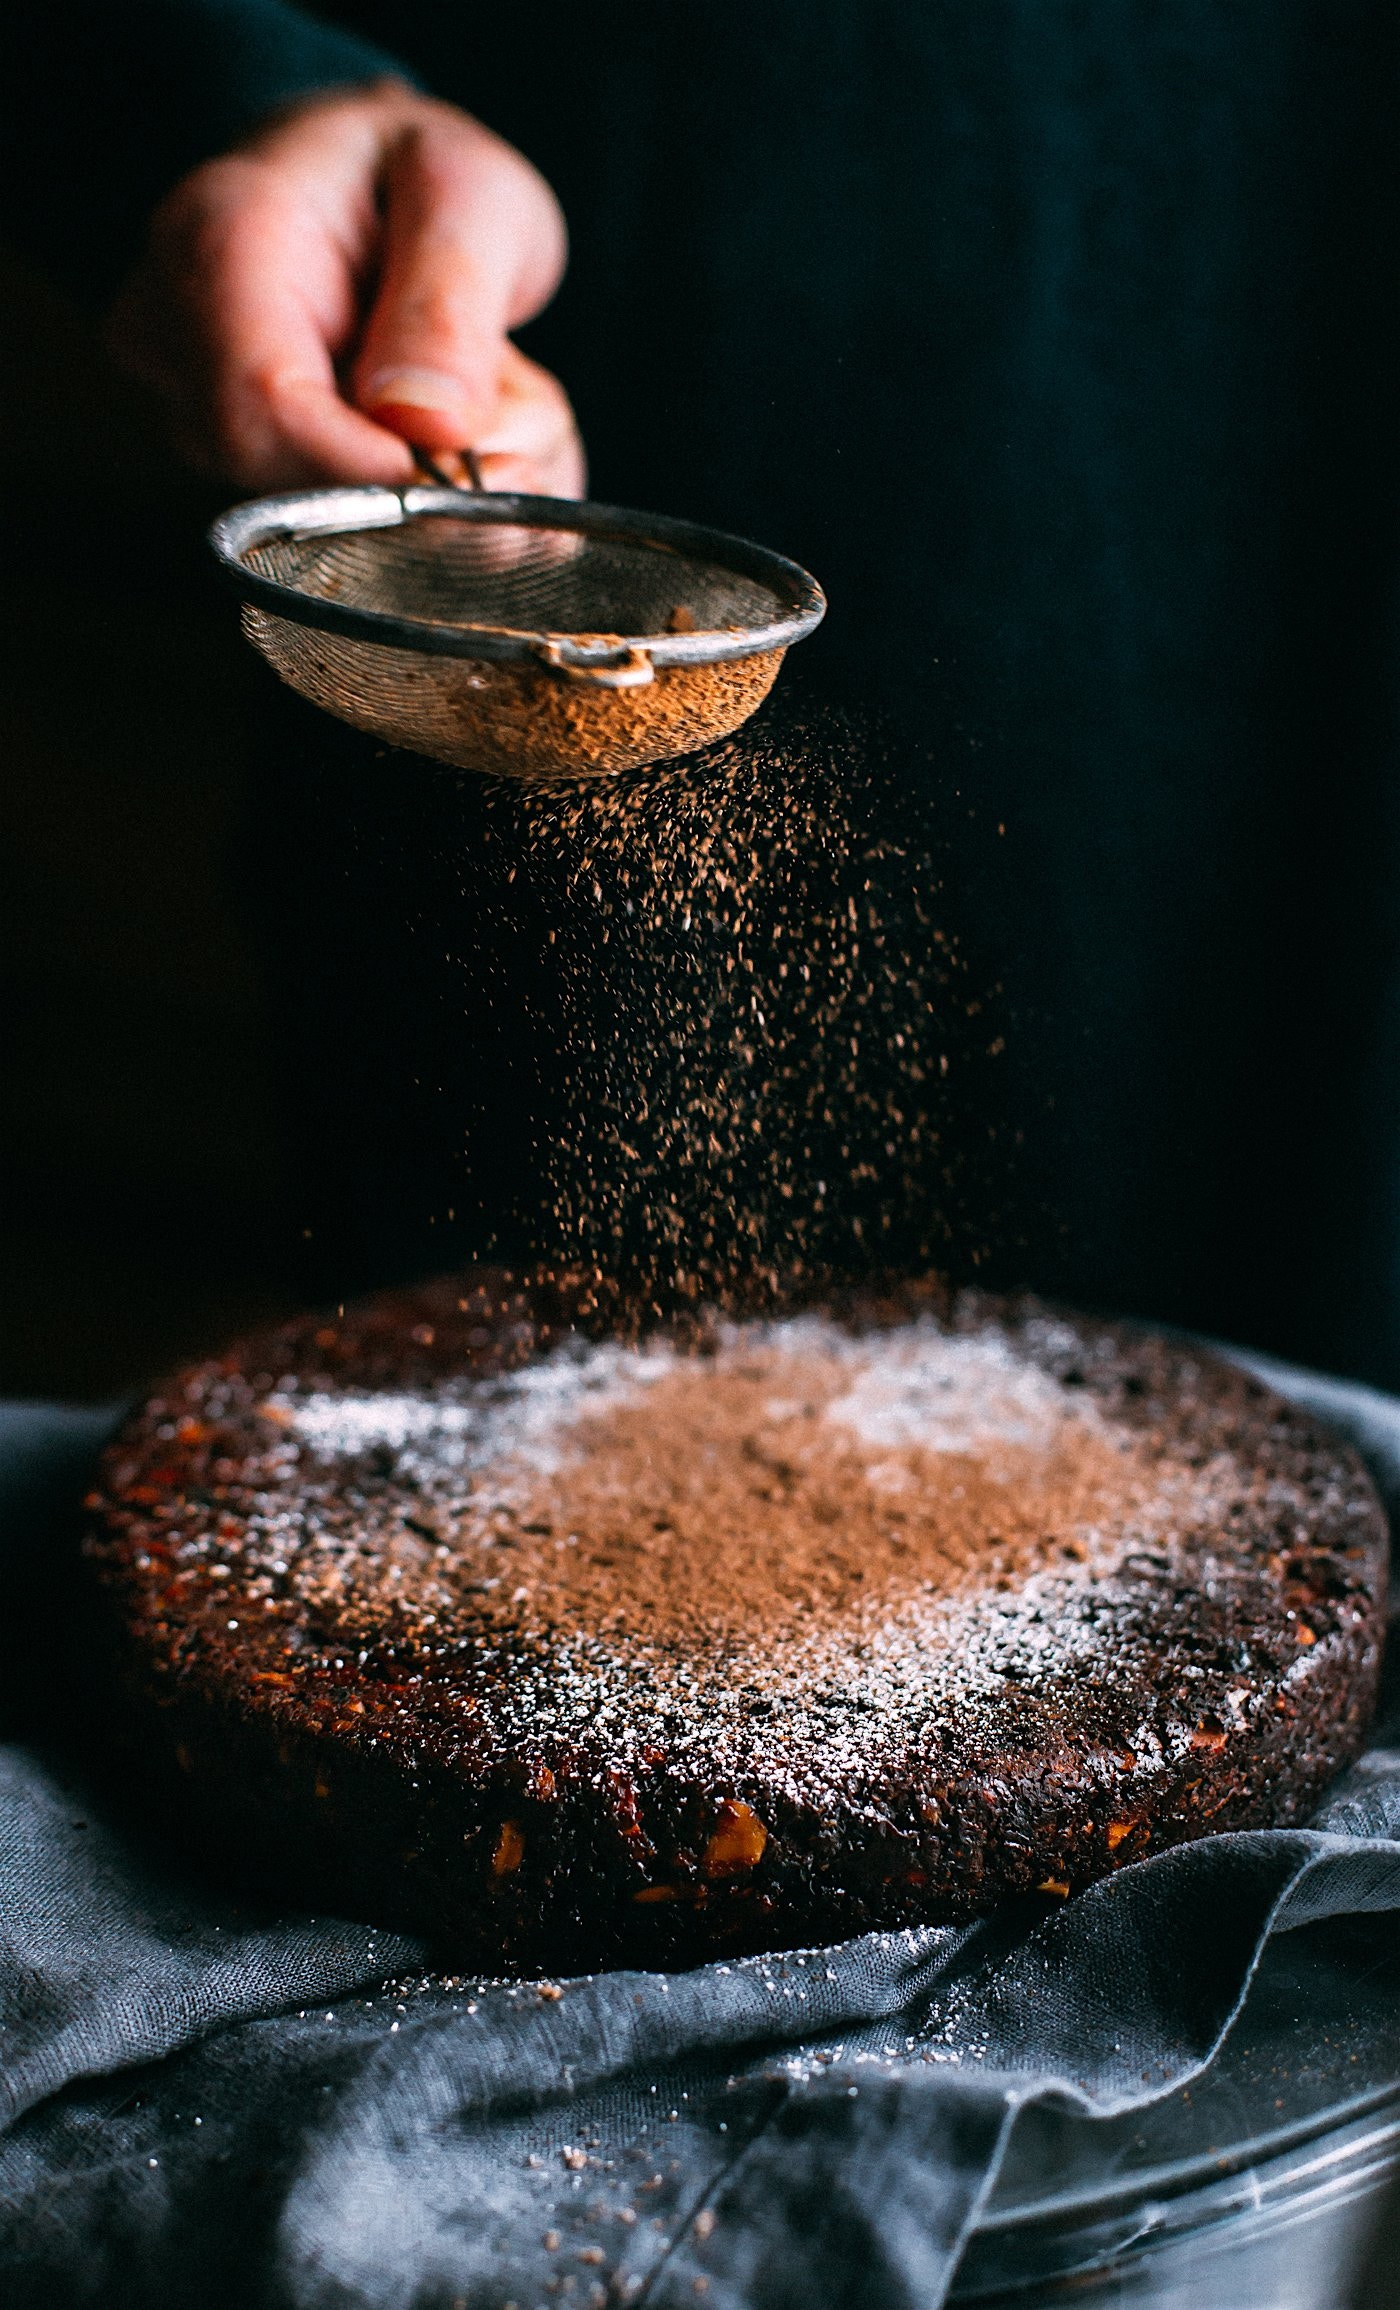
\includegraphics[width=0.2\textwidth]{gfx/05-cake} 
\end{wrapfigure}

Measurement is important. People who have attempted to bake a cake from scratch without measuring the ingredients will find, no doubt, that measurement is the difference between a sweet desert and a disaster. Just like in baking, measurement is important to a researcher. Measurement means the process by which key facts, attributes, concepts, and other phenomena are described. At its core, measurement is about defining the research project's terms in a precise and measurable way. Of course, measurement in business research is not quite as simple as using some predetermined or universally agreed-on tool, such as a measuring cup, but there are some basic tenants on which most researchers agree when it comes to measurement.\blfootnote{Photo by lindsay Cotter on Unsplash}


\subsection{What Do Researchers Measure?}

The question of what business researchers measure can be answered by asking what business researchers study. Researchers study a wide variety of business and marketing concepts, like corporate culture\cite{denison1990corporate}, the price elasticity of gasoline\cite{hughes2006evidence}, employee turnover\cite{hom1995employee}, and automobile ``lemons''\cite{akerlof1978market}. Each of these topics required measurements of various types and researchers had to determine the best way to do that. As you might have guessed, researchers will measure just about anything that they have an interest in investigating. 

In 1964, philosopher Abraham Kaplan wrote what has since become a classic work in research methodology, \textit{The Conduct of Inquiry}\cite{kaplan2017conduct}. In his text, Kaplan describes different categories of things that behavioral scientists observe. One of those categories, which Kaplan called ``observational terms,'' is probably the simplest to measure, and are the sorts of things that can be seen with the naked eye simply by looking at them. They are terms that ``lend themselves to easy and confident verification.'' If, for example, researchers wanted to know how the conditions of playgrounds differ across different neighborhoods, they could directly observe the variety, amount, and condition of equipment at various playgrounds.

Indirect observables, on the other hand, are less straightforward to assess. They are ``terms whose application calls for relatively more subtle, complex, or indirect observations, in which inferences play an acknowledged part. Such inferences concern presumed connections, usually causal, between what is directly observed and what the term signifies.'' If researchers conducted a study for which they wished to know a person's income, they could simply ask in an interview or a survey. Thus, they would have observed income, even if it was only observed indirectly. Birthplace might be another indirect observable. Researchers can ask study participants where they were born, but chances are good that they will not directly observe any of those people being born in the locations they report.

Sometimes the measures that we are interested in are more complex and more abstract than observational terms or indirect observables. Think about concepts like ethnocentrism, the way a person judges another person's culture, and how measuring that concept would be very challenging. In the same way, a concept like  ``bureaucracy'' would be very difficult to measure. In both cases, ethnocentrism and bureaucracy, the theoretical notions represent ideas whose meaning is known but the measurement of the concept may be nearly impossible. Kaplan referred to these more abstract things as \glspl{construct}. Constructs are ``not observational either directly or indirectly'' but they can be defined based on observables.

\subsection{How Do Researchers Measure?}

Measurement in business research is a process. It occurs at multiple stages of a research project: in the planning stage, in the data collection stage, and sometimes even in the analysis stage. 

As an example, imagine that the research question is: How do new college students cope with the adjustment to college? The first problem is to define ``cope'' in such a way that it can be measured. After that, the data collection phase can be designed to measure whatever ``cope'' means. After the data are collected then the analysis begins. Perhaps during the analysis phase an unexpected facet of coping is discovered and that may mean that the measures taken would need to be revisited to allow for that facet. Once the analysis is complete then there are certain decisions concerning the report. Perhaps one method of coping is determined to be more effective than others so the report may contain a recommendation that future research be conducted that measures just that one method of coping. The point is that measurement considerations are important throughout the research project.

The measurement process could also involve multiple stages. Starting with identifying and defining key terms to determining how to observe and measure them to assessing the quality of the measurements, there are multiple steps involved in the measurement process. An additional step in the measurement process involves deciding what type of data\marginpar{Data types are discussed on page \pageref{ch05:data}.} will be collected and an appropriate analysis process for those particular types of data elements. 

\section{Conceptualization}

One of the first steps in the measurement process is conceptualization, which is defining the terms of the project as clearly as possible. Keep in mind that terms mean only what the researcher determines, nothing more and nothing less.

A \textit{concept} is the notion or image that is conjured up when the researcher thinks of some cluster of related observations or ideas. For example, masculinity is a concept. A researcher thinking about that concept may imagine some set of behaviors and perhaps even a particular style of self presentation. Of course, not everyone will conjure up that same set of ideas or images: in fact, there are many possible ways to define the term. While some definitions may be more common or have more support than others, there is not one true, always-correct-in-all-settings definition for ``masculine'' and that definition may well change over time, from culture to culture, and even from individual to individual, as explained by George Mosse\cite{george1996image}. This is why defining concepts is so important before any data gathering begins.

It may seem unreasonable for a researcher to define a term for which there is no single, correct definition. Unfortunately, this will be a problem for most concepts measured in a business or marketing study. William Clinton, the 42\textsuperscript{d} President of the United States, famously stated ``It depends upon what the meaning of the word 'is' is.''\footnote{This was widely reported in the press and can be easily found on-line, including YouTube videos of him making that statement.} Without understanding how a researcher has defined the key concepts it would be impossible to understand the importance of the findings.

Defining concepts is an early part of the process of measurement called conceptualization, which involves writing out clear, concise definitions for key concepts. Brainstorming may help to conceptualize a topic, but it would also make sense to consult existing research and theory to see if other scholars have already defined the concepts of interest. This does not necessarily mean that their definitions are correct, but understanding how concepts have been defined in the past will help with a current project. Conceptualization is not as simple as merely applying a definition from a dictionary, it requires careful consideration and evaluating alternative concepts.

One important decision while conceptualizing constructs is specifying whether they are unidimensional or multidimensional. Unidimensional constructs are those that are expected to have a single underlying dimension and can be measured using a single measure or test. Examples include simple constructs such as a person's weight, wind speed, and even complex constructs like self-esteem (if self-esteem is conceptualized as consisting of a single dimension, which of course, may be unrealistic). Multidimensional constructs consist of two or more underlying dimensions. For instance, if a person's academic aptitude is conceptualized as consisting of two dimension, mathematical and verbal ability, then academic aptitude is a multidimensional construct. Each of the underlying dimensions in this case must be measured separately by using different tests for mathematical and verbal ability, and then combine the two scores, possibly in a weighted manner, to create an overall value for the academic aptitude construct.

Before moving on to the next steps in the measurement process, it would be wise to consider one of the dangers associated with conceptualization. While it is important to consult prior scholarly definitions of key concepts, it would be wrong to assume that those definitions are any more real than whatever current definitions are generated by the researcher. It would also be wrong to assume that just because definitions exist for some concept that the concept itself exists beyond some abstract idea. This idea, assuming that abstract concepts exist in some concrete way is known as reification.

To better understand reification, take a moment to think about the concept of ``family.'' This concept is central to sociological thinking, but it is an abstract term. If researchers were interested in studying this concept, they would consult prior research to understand how the term has been conceptualized by others. But they should also question past conceptualizations. Today's conceptualization of ``family'' would be very different from one that was used a hundred years ago. The point is that terms mean nothing more and nothing less than whatever definition is assigned by the researcher. Sure, it makes sense to come to some agreement about what various concepts mean. Without that agreement, it would be difficult to navigate through everyday living. But at the same time, it is important to remember that a society has assigned those definitions and that they are no more real than any other, alternative definition a researcher might choose to assign.

\section{Operationalization}

Once a theoretical construct is defined, indicators for measuring the construct are defined in a process called operationalization. For instance, if an unobservable theoretical construct such as socioeconomic status is defined as the level of family income then it can be operationalized using an indicator that asks respondents the question: what is your annual family income? Given the high level of subjectivity and imprecision inherent in social science constructs, most (except a few demographic constructs such as age, gender, education, and income) are measured using multiple indicators.

\begin{figure}[H]
	\centering
	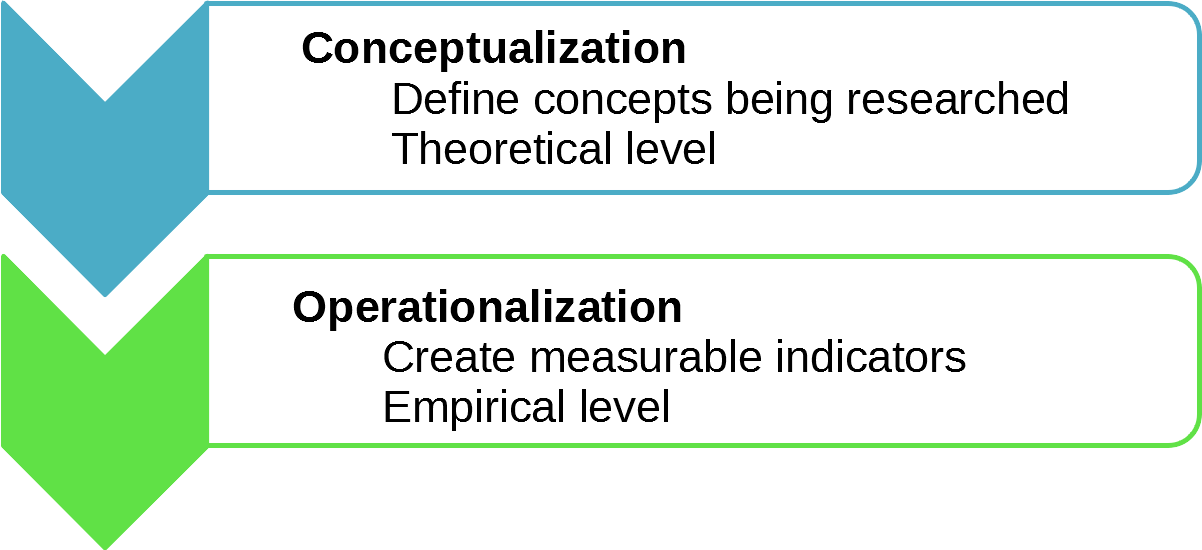
\includegraphics[width=\maxwidth{.95\linewidth}]{gfx/05-ConceptVsOper}
	\caption{Conceptualization Vs. Operationalization}
	\label{05:fig02}
\end{figure}

Indicators operate at the empirical level in contrast to constructs, which are conceptualized at the theoretical level. The combination of indicators at the empirical level representing a given construct is called a \gls{variable}, and those may be independent, dependent, mediating, or moderating, depending on how they are employed in a research study. Also each indicator may have several attributes (or levels) and each attribute represent a value. For instance, a ``gender'' variable may have two attributes: male or female. Likewise, a customer satisfaction scale may be constructed to represent five attributes: ``strongly dissatisfied,'' ``somewhat dissatisfied,'' ``neutral,'' ``somewhat satisfied'' and ``strongly satisfied.'' 

Variables may be quantitative (numeric) or qualitative (textual). Quantitative data can be analyzed using techniques like regression or structural equation modeling while qualitative data uses techniques like coding. Note that many variables in business research are qualitative, even when represented in a quantitative manner. For instance, a customer satisfaction indicator with five attributes: strongly dissatisfied, somewhat dissatisfied, neutral, somewhat satisfied, and strongly satisfied, can assign the numbers $ 1-5 $ respectively for these five attributes, so that we can use sophisticated statistical tools for quantitative data analysis. However, note that the numbers are only labels associated with respondents' personal evaluation of their own satisfaction, and the underlying variable (satisfaction) is still qualitative even though it is represented numerically.

Indicators may be reflective or formative. A reflective indicator is a measure that ``reflects'' an underlying construct. For example, if religiosity is defined as a construct that measures how religious a person is, then attending religious services may be a reflective indicator of religiosity. A formative indicator is a measure that ``forms'' or contributes to an underlying construct. Such indicators may represent different dimensions of the construct of interest. For instance, if religiosity is defined as composed of a belief dimension, a devotional dimension, and a ritual dimension, then indicators chosen to measure each of these different dimensions will be considered formative indicators. Unidimensional constructs are measured using reflective indicators (even though multiple reflective indicators may be used for measuring abstruse constructs such as self-esteem), while multidimensional constructs are measured as a formative combination of the multiple dimensions, even though each of the underlying dimensions may be measured using one or more reflective indicators.

It is important to keep in mind that the process of coming up with indicators cannot be arbitrary or casual. One way to avoid taking an overly casual approach in identifying indicators is to turn to prior theoretical and empirical work. Theories will point to relevant concepts and possible indicators while empirical work will detail specific examples of how key concepts have been measured in the past. One final important detail to think about when deciding on indicators is the strategy you will use for data collection. A survey implies one way of measuring concepts while field research implies a very different way. The data-collection strategy employed will play a major role in shaping how concepts are operationalized.

\section{Measurement Quality}

The previous section examined some of the difficulties with measuring constructs. What makes the task more challenging is that sometimes these constructs are imaginary concepts (i.e., they don’t exist in reality), and multi-dimensional (in which case, we have the added problem of identifying their constituent dimensions). Hence, it is not adequate just to measure constructs using any scale, the scales must be tested to ensure that: 

\begin{enumerate}
	\item they measure the construct consistently and precisely (i.e., the scales are ``reliable'') and 

	\item they actually measure the construct being investigated (i.e., the scales are ``valid''). 
\end{enumerate}

Reliability, the consistency of a measure, and validity, the efficacy of a measure, are the two yardsticks against which the accuracy of measurements are evaluated in scientific research. A measure can be reliable but not valid if it is measuring consistently but it is the wrong construct. Likewise, a measure can be valid but not reliable if it is measuring the right construct but not doing so in a consistent manner. Using the analogy of a shooting target, as shown in Figure \ref{05:fig03}, a measure that is both reliable and valid is like a group that is tightly clustered near the center of the target. A measure that is reliable but not valid is like a group that is tightly clustered but off-center. A measure that is valid but not reliable is a group that is widely scattered but centered. Finally, a measure that is neither reliable nor valid is like a group that is widely scattered and off-center. 

\begin{figure}[H]
	\centering
	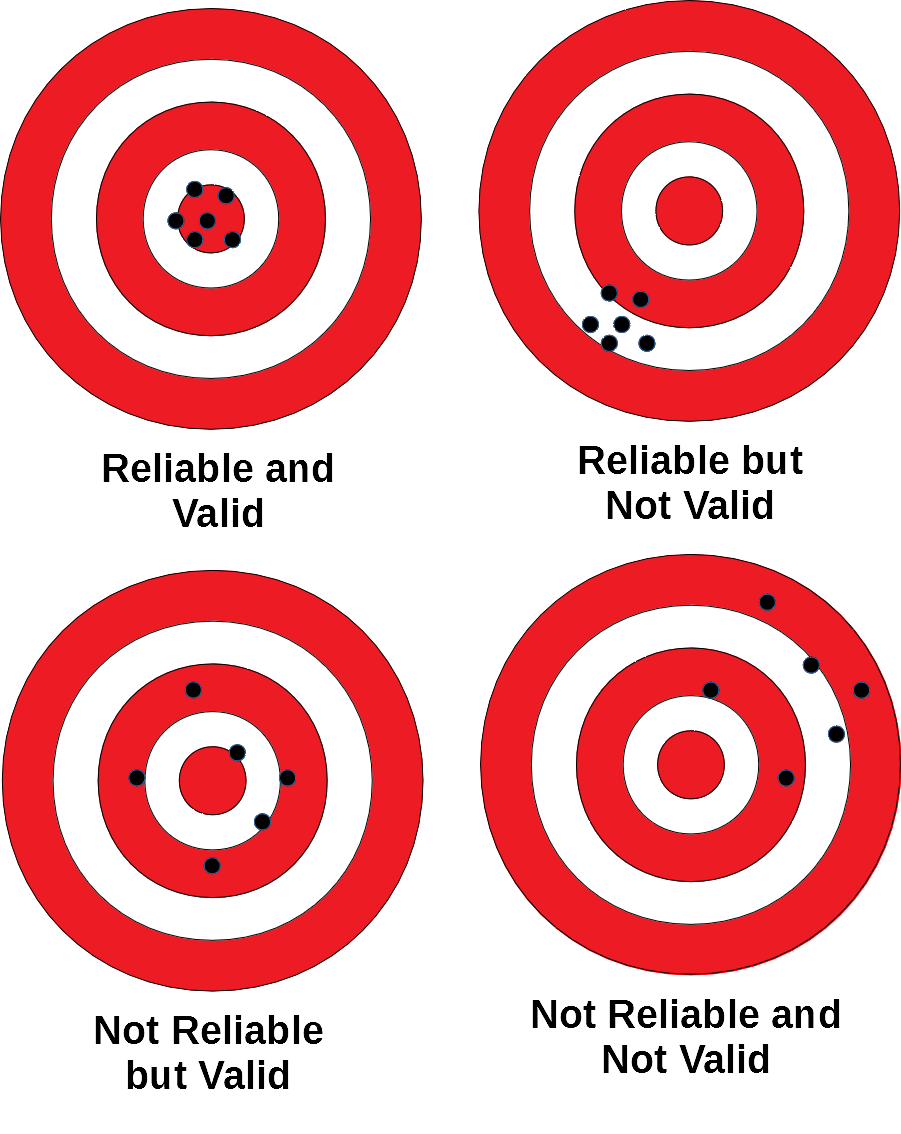
\includegraphics[width=\maxwidth{.95\linewidth}]{gfx/05-Targets}
	\caption{Reliability Analogy}
	\label{05:fig03}
\end{figure}

\subsection{Reliability}

\Gls{reliability} ``...is the extent to which measurements are repeatable – when different persons perform the measurements, on different occasions, under different conditions, with supposedly alternative instruments which measure the same thing.''\cite{drost2011validity}

Any score obtained by a measuring instrument (the observed score) is composed of both the ``true'' score, which is the score that a person would have received if the measurement were perfectly accurate, and the ``error'' in the measurement process. Imagine a simple example, a bathroom scale. If a person's true weight were $ 150 $ pounds then, ideally, the scale would read $ 150 $ every time that person stepped on the scale. The scale's reliability is the consistency of its output from one day to the next. If a person stepped on the scale one day and it read $ 160 $ but the next day it read $ 140 $ then the scale would not be a reliable instrument.

There are two types of reliability errors that researchers need to understand. First is systematic error, one that is caused by the system and is predictable. For example, the if the bathroom scale mentioned above constantly read five pounds heavy that would be an error, but it would be one that is consistent and could be corrected in the research data. That is an example of a systematic error. The second type of error is a random error. If the bathroom scale were accurate but the person reading it one day read $ 151 $ and the next as $ 149 $ then that would be a random error. Random errors cannot be corrected but tend to cancel out due to the random nature of the error (sometimes the reading will be a bit high and other times low), especially if there are many data points.

Unreliable measurements in business research could be for several reasons. One is the researcher's subjectivity. For example, if employee morale in a firm is being measured by watching whether the employees smile at each other, whether they make jokes, and so forth, then different observers may infer different measures of morale if they are watching the employees on a very busy day (when they have no time to joke or chat) or a light day (when they are more jovial or chatty). Two observers may also infer different levels of morale on the same day, depending on what they view as a joke and what is not. ``Observation'' is a qualitative measurement technique. 

Sometimes, reliability may be improved by using quantitative measures. Counting the number of grievances filed over one month as a measure of (the inverse of) morale. Of course, grievances may or may not be a valid measure of morale, but it is less subject to human subjectivity, and therefore more reliable. 

A second source of unreliable observation is asking imprecise or ambiguous questions. For instance, if people are asked to report their salary some may state a monthly salary, some an annual salary, and some even an hourly wage. Thus, the resulting observations will be divergent and unreliable. 

A third source of unreliability is asking questions about issues that respondents are not very familiar with or care about, such as asking an American college graduate about Canada's relationship with Slovenia or asking a Chief Executive Officer to rate the effectiveness of his company's technology strategy (which was likely delegated to a technology executive).

To improve reliability, start by replacing subjective data collection techniques (observation) with those that are more objective (questionnaire), ask respondents only questions that they may know or care about, avoid ambiguous items (e.g. clearly indicate annual salary), and simplify the wording in indicators. While these strategies can improve the reliability of measurements, instruments must still be tested for reliability using techniques like the following.

\begin{itemize}
	\item \textbf{Inter-rater reliability}. Inter-rater reliability, also called inter-observer reliability, is a measure of consistency between two or more independent raters (observers) of the same construct. Usually, this is assessed in a pilot study and can be done in two ways, depending on the level of measurement being used. If the measure is categorical, a set of all categories is defined, raters check off which category each observation falls in, and the percentage of agreement between the raters is used as an estimate of inter-rater reliability. For instance, if there are two raters rating $ 100 $ observations into one of three possible categories, and their ratings match for $ 75\% $ of the observations, then inter-rater reliability is $ 0.75 $. If the measure is interval or ratio scaled (e.g., classroom activity is being measured once every five minutes by two raters on one to seven scale), then a simple correlation between measures from the two raters can also serve as an estimate of inter-rater reliability.

	\item \textbf{Test-retest reliability}. Test-retest reliability is a measure of consistency between two measurements (tests) of the same construct administered to the same sample at two different points in time. If the observations have not changed substantially between the two tests, then the measure is reliable. The correlation in observations between the two tests is an estimate of test-retest reliability. Note here that the time interval between the two tests is critical. Generally, the longer is the time gap, the greater is the chance that the two observations may change during this time (due to random error), and the lower will be the test-retest reliability.

	\item \textbf{Split-half reliability}. Split-half reliability is a measure of consistency between two halves of a construct measure. For instance, if you have a ten-item measure of a given construct, randomly split those ten items into two sets of five (unequal halves are allowed if the total number of items is odd), and administer the entire instrument to a sample of respondents. Then, calculate the total score for each half for each respondent, and the correlation between the total scores in each half is a measure of split-half reliability. The longer the instrument, the more likely it is that the two halves of the measure will be similar (since random errors are minimized as more items are added), and hence, this technique tends to systematically overestimate the reliability of longer instruments.

	\item \textbf{Internal consistency reliability}. Internal consistency reliability is a measure of consistency between different items of the same construct. If a multiple-item construct measure is administered to respondents, the extent to which respondents rate those items in a similar manner is a reflection of internal consistency. This reliability can be estimated in terms of average inter-item correlation, average item-to-total correlation, or more commonly, \textit{Cronbach’s alpha}. 

\end{itemize}

\subsection{Validity}

\Gls{validity} is concerned with the meaningfulness of research results. In brief, does the research actually measure what it was purported to measure? For example, does the Scholastic Aptitude Test (SAT) actually predict the likelihood of a high school student successfully completing college?\cite{drost2011validity} There are numerous types of validity found in the literature, but they generally form two large groups: Measurement Validity (the measurement should accurately reflect the construct) and Hypothesis Validity (the hypotheses should accurately reflect the construct).

\subsubsection{Measurement Validity}

The \textit{theoretical} assessment of validity focuses on how well an abstract construct is translated into an operational measure, which is called \gls{translationalvalidity}, and divided into two sub-types: face and content validity. Translational validity is typically assessed using a panel of expert judges who rate each item (indicator) on how well it fits the conceptual definition of that construct along with a qualitative technique called \textit{Q-method}, as explained by Pnina Shinebourne\cite{shinebourne2009using}.

The \textit{empirical} assessment of validity examines how well a given measure relates to one or more external criterion, based on empirical observations. This type of validity is called \gls{criterionvalidity}, which is divided into four sub-types: convergent, discriminant, concurrent, and predictive. While translation validity examines whether a measure is a good reflection of its underlying construct, criterion-related validity examines whether a given measure behaves the way it should, given the theory of that construct. The distinction between theoretical and empirical assessment of validity is illustrated in Figure \ref{05:fig04}. However, both approaches are needed to adequately ensure the validity of measures in business research.

\begin{figure}[H]
	\centering
	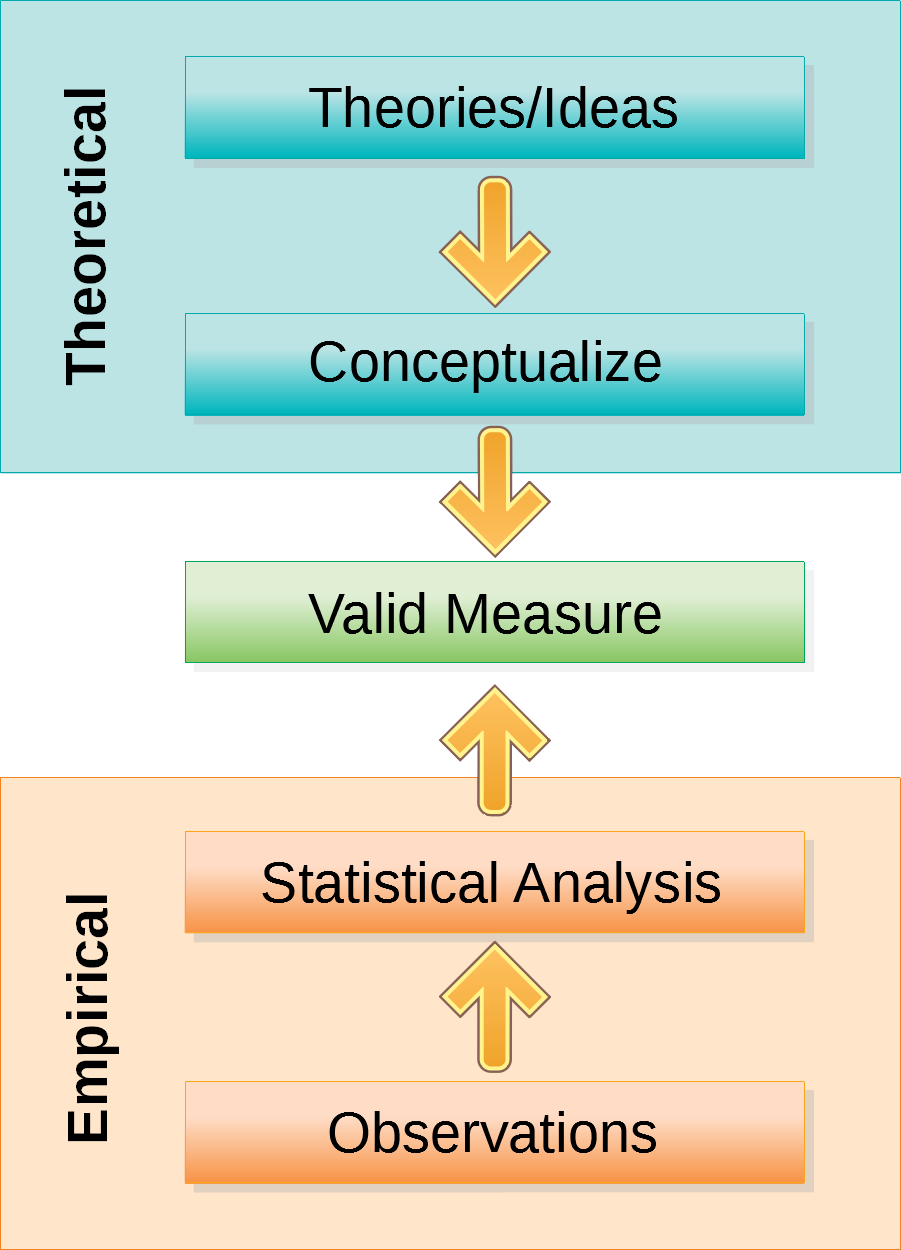
\includegraphics[width=\maxwidth{.95\linewidth}]{gfx/05-AssessValidity}
	\caption{Assessing Theoretical and Empirical Validity}
	\label{05:fig04}
\end{figure}

\paragraph{Translational Validity}

\begin{description}
	\item[\Gls{facevalidity}] refers to whether an indicator seems to be a reasonable measure of its underlying construct ``on its face.'' For instance, the frequency of attendance at religious services seems to make sense as an indication of a person's religiosity without a lot of explanation. Hence this indicator has face validity. However, if we were to suggest how many books were checked out of an office library as a measure of employee morale, then such a measure would probably lack face validity because it does not seem to make much sense. Interestingly, some of the popular measures used in organizational research appear to lack face validity. For instance, absorptive capacity of an organization (how much new knowledge can it assimilate for improving organizational processes) has often been measured by research and development intensity (\ie, R\&D expenses divided by gross revenues). Research that includes constructs that are highly abstract or are hard to conceptually separate from each other (\eg, compassion and empathy), it may be worthwhile to use a panel of experts to evaluate the face validity of the measures.

	\item[\Gls{contentvalidity}] is an assessment of how well a measure matches the content domain of the construct being measured. For instance, to measure the construct ``satisfaction with restaurant service,'' then the content domain should include the quality of food, courtesy of wait staff, duration of wait, and the overall ambiance of the restaurant (i.e., whether it is noisy, smoky, etc.). The project should measure the extent to which a restaurant patron is satisfied with the quality of food, courtesy of wait staff, the length of wait, and the restaurant's ambiance. Of course, this approach assumes the researcher can create a detailed description of the content domain, which may be difficult for complex constructs such as self-esteem or intelligence. As with face validity, an expert panel of judges may be employed to examine content validity of constructs.
\end{description}

\paragraph{Criterion-Related Validity}

\begin{description}

	\item[\Gls{convergentvalidity}] refers to the closeness with which a measure, or group of measures, relates to (or converges on) the construct that it is purported to measure. Convergent validity can be established by comparing the observed values of one indicator with those of other indicators to attempt to find high correlation between those indicators. Compare this to discriminant validity.
	
	\item[\gls{discriminantvalidity}] refers to the degree to which a measure does not measure (or discriminates from) other constructs that it is not supposed to measure. Usually, convergent validity and discriminant validity are assessed jointly for a set of related constructs. For example, if an organization's knowledge is related to its performance then a measure of organizational knowledge must actually measure organizational knowledge (convergent validity) and not organizational performance (discriminant validity). Discriminant validity is established by demonstrating that indicators of one construct are dissimilar from (i.e., have low correlation with) other constructs.

	\item[\Gls{concurrentvalidity}] examines how well a measure of one outcome relates to another outcome that is presumed to occur simultaneously. For instance, do students' scores in a calculus class correlate well with their scores in a linear algebra class? Since both are mathematics classes it would be presumed that there is high concurrent validity between scores in those classes. 
	
	\item[\Gls{predictivevalidity}] is the degree to which a measure successfully predicts a future outcome. For example, a standardized test score (\eg, \textit{Scholastic Aptitude Test}) can be used to predict a student's academic success in college. Concurrent and predictive validity are not often considered in empirical business research.

\end{description}

\subsubsection{Hypothesis Validity}

In general, four types of hypothesis validity are referred to in the literature.

\begin{description}
	\item[Internal validity]. Internal validity, also called causality, examines whether the observed change in a dependent variable is caused by a corresponding change in hypothesized independent variable and not by variables extraneous to the research context. Causality requires three conditions: 1) covariation of cause and effect (if cause happens then effect also happens and if cause does not happen effect does not happen), 2) temporal precedence (cause must precede effect in time), and 3) lack of plausible alternative explanation (or spurious correlation). Certain research designs, such as laboratory experiments, are strong in internal validity since researchers can manipulate the independent variable (cause) via a treatment and observe the effect (dependent variable) of that treatment after a certain point in time while controlling for the effects of extraneous variables. Other designs, such as field surveys, are poor in internal validity because researchers cannot manipulate the independent variable (cause) and because cause and effect are measured at the same point in time which defeats temporal precedence making it equally likely that the effect actually brought about the presumed cause rather than the reverse. 
	
	%There is a nice graphic of validity and the ``cone'' of types of validity, Anol p 45.
	
	\item[External Validity]. External validity, or generalizability, refers to whether the observed associations can be generalized from the sample to the population (population validity), or to entities outside the population (ecological validity). For instance, if results drawn from a sample of financial firms in the United States can be generalized to the population of all financial firms it would have strong population validity and if to other types of firms it would have strong ecological validity. Survey research, where data are sourced from a wide variety of individuals, firms, or other units of analysis, tends to have broader generalizability than laboratory experiments where artificially contrived treatments and strong control over extraneous variables render the findings less generalizable to real-life settings where treatments and extraneous variables cannot be controlled. \marginpar{Some researchers claim that increased external validity leads to decreased internal validity and vice-versa, but this is not always true. Some research designs, such as multiple case studies, have high degrees of both internal and external validities.}
	
	\item[Construct Validity]. Construct validity examines how well a given measurement scale is measuring the theoretical construct that it is designed to measure. One frequent problem with construct validity is simply defining the construct in such a way that it is measurable. As one example, ``property ownership'' is a construct of a market economy explained by Robert Reich\cite{reich2016saving}. That is, the fact that people can own property drives a local economy. But this construct relies on a number of external forces that cannot be controlled, such as local politics (a city's eminent domain can take a person's property) and the value of the property on the open market. Measuring the influence of property ownership on a local economy (the construct) would be very difficult since there are so many confounding variables. 
	
	\item[Statistical Conclusion]. Statistical conclusion validity examines the extent to which conclusions derived from a statistical procedure are valid. For example, it examines whether the right statistical method was used and whether the variables meet the assumptions of that statistical test (such as sample size or distributional requirements). 
	
\end{description}


\subsection{Improving Internal and External Validity}

The best research designs are those that can assure high levels of internal and external validity. Such designs would guard against spurious correlations, inspire greater faith in the hypotheses testing, and ensure that the results drawn from a small sample are generalizable to the population at large. The internal validity of research designs and can be improved using four methods: 1) manipulation, 2) elimination, 3) inclusion, and 4) randomization.

\begin{enumerate}
	\item Manipulation involves the researcher manipulating the independent variables in one or more ways (called ``treatments''), and compares the effects of the treatments against a control group where subjects do not receive the treatment. Treatments may include a new drug or different dosage of drug (for treating a medical condition), a new teaching style (for education), and so forth. This type of control can be achieved in experimental or quasi-experimental designs but not in non-experimental designs such as surveys. 
	
	\item Elimination relies on eliminating extraneous variables by holding them constant across treatments, such as by restricting the study to a single gender or a single socioeconomic status. 
	
	\item Inclusion is the process of separately estimating the effects of spurious variables on the dependent variable. As an example, consider the process of estimating the effect of gender on a marketing study. Inclusion techniques allow for greater generalizability of the study but also require substantially larger samples. 
	
	\item Randomization is aimed at canceling out the effects of extraneous variables through a process of random sampling. Two types of randomization are: 1) random selection, where a sample is selected randomly from a population, and 2) random assignment, where subjects selected in a non-random manner are randomly assigned to treatment groups. Randomization also improves external validity, allowing inferences drawn from the sample to be generalized to the population from which the sample is drawn; however, generalizability across populations is harder to ascertain since populations may differ on multiple dimensions and only a few of those dimensions can be controlled.
	
\end{enumerate}

\section{Summary}\label{ch06:summary}

\begin{itemize}
	\setlength{\itemsep}{0pt}
	\setlength{\parskip}{0pt}
	\setlength{\parsep}{0pt}
	
	\item In social science, our variables can be one of four different levels of measurement: nominal, ordinal, interval, or ratio.
	\item Indexes and typologies allow us to account for and simplify some of the complexities in our measures.
	
\end{itemize}

%%*****************************************
\chapter{Data}\label{06:data}
%*****************************************
%TODO Status: pre-draft

\begin{wrapfigure}{r}{0.4\textwidth}
	\label{06:fig01} 
	\centering
	
\includegraphics[width=0.4\textwidth]{gfx/06-data} 
\end{wrapfigure}
Data are\footnote{The word ``data'' is plural and is treated that way in this text even though modern usage seems to be trending toward a singular form.} a collection of facts about some topic. As examples, a ``customer loyalty'' program gathers data from customers on how often they shop, what they purchase on each trip, what time of day they typically shop, and all sorts of other data. When data are interpreted in some way they become information. The types of analyses that can be done with data are limited by the types of data involved. The purpose of this chapter is to introduce various concepts about data and show how they can be analyzed.\footnote{Photo by Mika Baumeister on Unsplash}

\subsection{Types of Data}

Psychologist Stanley Smith Stevens defined four generic types of data\cite{stevens1946theory}. 

\begin{itemize}
	
	\item \textbf{\Gls{qualitativedata}} groups observations into a limited number of categories; for example, type of pet (cat, dog, bird, etc.) or place of residence (Arizona, California, etc.). Because qualitative data do not have characteristics like means or standard deviations, they are analyzed using non-parametric tests, like Kruskal-Wallis H and Mann-Whitney U. Qualitative data can be further divided into two sub-types, nominal and ordinal.
	
	\begin{itemize}
		\item \textbf{\Gls{nominaldata}} are categories that do not overlap and have no meaningful order, they are merely labels for attributes. Examples of nominal data include occupations (custodial, accounting, sales, etc.) and blood type (A, B, AB, O). A special subcategory of nominal data is binary, or dichotomous, where there are only two possible responses, like ``yes'' and ``no''. Nominal data are sometimes stored in a database using numbers but they cannot be treated like numeric data. For example, binary data, like ``Do you rent or own your home?'' can be stored as ``1 = rent, 2 = own'' but the numbers in this case have no numeric significance and could be replaced by words like ``Rent'' and ``Own.''
		
		\item \textbf{\Gls{ordinaldata}} are categorical data but, unlike nominal, the categories imply some sort of order (which is why it is called ``ordinal'' data). One example of ordinal data is the ``star'' rating system for movies. It is clear that a five-star movie is somehow better than a four-star movie but there is no way to quantify the difference between those two categories. As another example, it is common for hospital staff members to ask patients to rate their pain level on a scale of one to ten. If a patient reports a pain level of ``seven'' but after some sort of treatment later reports a pain level of ``five'' then the pain has clearly decreased but it would be impossible to somehow quantify the exact difference in those two levels. Ordinal scales are most commonly used with Likert-type survey questions where the responses are selections like ``Strongly Agree'', ``Agree'', ``Neutral'', ``Disagree'', ``Strongly Disagree''. Ordinal data are also used when numeric data are grouped. For example, if a dataset included respondents' ages then those numbers could be grouped into categories like ``$ 20-29 $'' and ``$ 30-39 $.'' Those groups would typically be stored in the dataset as a single number so maybe ``$ 2 $'' would represent the ages ``$ 20-29 $,'' which would be ordinal data.
	\end{itemize}
	
	\item \textbf{\Gls{quantitativedata}} are numbers, typically counts or measures, like a person's age, a tree's height, or a truck's weight. Quantitative data are measured with scales that have equal divisions so the difference between any two values can be calculated. Quantitative data are discrete if they are represented by integers, like the count of words in a document, or continuous if they are represented by fractional numbers, like a person's height. Because quantitative data includes characteristics like means and standard deviations, they are analyzed using parametric tests, like T-tests and Analysis of Variance (ANOVA). Quantitative data can be further divided into two sub-types, interval and ratio.
	
	\begin{itemize}
		\item \textbf{\Gls{intervaldata}} use numbers to represent quantities where the distance between any two quantities can be calculated but there is no true zero point on the scale. One example is a temperature scale where the difference between $ 80 $\textdegree and $ 90 $\textdegree is the same as the difference between $ 60 $\textdegree and $ 70 $\textdegree. It is important to note that interval data do not include any sort of true zero point, thus zero degrees Celsius does not mean ``no temperature,'' and without a zero point it is not reasonable to make a statement like $ 20 $\textdegree is twice as hot as $ 10 $\textdegree.
		
		\item \textbf{\Gls{ratiodata}} use numbers to describe a specific measurable distance between two quantities; however, unlike interval data, ratio data have a true zero point. A good example of ratio data is the sales report for an automobile dealership. Because the data are a simple count of the number of automobiles sold it is possible to compare on month with another. Also, since the scale has a true zero point (it is possible to have zero sales) it is possible to state that one month had twice the sales of another.
	\end{itemize}
\end{itemize}

\section{Rating Scale}

When working with qualitative data, it is important for researchers to determine a rating scale, also called levels of measure, to record data gathered about any one attribute. For example, male-female-other, M-F-O, and $ 1 $-$ 2 $-$ 3 $ are three potential rating scales for the attribute \textit{gender}. A researcher could use any of these scales, or devise a completely different one, as long as the scale is used consistently throughout the entire research project. It is easy to imagine that many rating scales exist but the most common ones are \textit{binary}, \textit{Likert}, \textit{semantic differential}, and \textit{Guttman}. 

\begin{description}
	\item[Binary] Binary scales are nominal scales consisting of binary items that assume one of only two possible values, such as yes or no, true or false, and so on. For example, a typical binary scale for a ``political activism'' construct may consist of the six binary items shown in Table \ref{tab06.02}. Each item in this scale is a binary item, and the total number of ``yes'' indicated by a respondent (a value from $ 0 $ to $ 6 $) can be used as an overall measure of that person's political activism. Binary scales can also employ other values, such as male or female for gender, full-time or part-time for employment status, and so forth. If an employment status item is modified to allow for more than two possible values (e.g., unemployed, full-time, part-time, and retired), it is no longer binary, but still remains a nominal scaled item.
	
	\begin{table}[H]
		\centering
		\begin{tabularx}{0.95\linewidth}{p{0.70\linewidth}p{0.09\linewidth}p{0.09\linewidth}}
			\toprule
			\textbf{Question} & \textbf{Yes} & \textbf{No} \\
			\midrule
			Have you ever written a letter to a public official? & $ \bigcirc $ & $ \bigcirc $ \\ 
			Have you ever signed a political petition? & $ \bigcirc $ & $ \bigcirc $ \\ 
			Have you ever donated money to a political cause? & $ \bigcirc $ & $ \bigcirc $ \\ 
			Have you ever donated money to a candidate running for public office? & $ \bigcirc $ & $ \bigcirc $ \\ 
			Have your ever written a political letter to the editor of a newspaper?& $ \bigcirc $ & $ \bigcirc $ \\ 
			Have you ever persuaded someone to change his/her voting plans? & $ \bigcirc $ & $ \bigcirc $ \\ 
			\bottomrule
		\end{tabularx}
		\caption{Political activism binary scale}
		\label{tab06.02}
	\end{table}
	
	\item[Likert] Designed by Rensis Likert, this is a very popular rating scale for measuring ordinal data in business research. This scale includes Likert items that are simply-worded statements to which respondents can indicate their extent of agreement or disagreement on a five or seven-point scale ranging from ``strongly disagree'' to ``strongly agree.'' A typical example of a six-item Likert scale for the ``employment self-esteem'' construct is shown in table \ref{tab06.03}. Likert scales are summated scales, that is, the overall scale score may be a summation of the attribute values of each item as selected by a respondent.
	
	\begin{table}[H]
		\centering
		\begin{tabularx}{0.95\linewidth}{p{0.35\linewidth}p{0.10\linewidth}p{0.08\linewidth}p{0.07\linewidth}p{0.07\linewidth}p{0.08\linewidth}}
			\toprule
			{\footnotesize Statement} & {\footnotesize Strongly disagree} & {\footnotesize Disagree} & {\footnotesize Neutral} & {\footnotesize Agree} & {\footnotesize Strongly agree} \\
			\midrule
			{\footnotesize I feel good about my job} & $ \bigcirc $ & $ \bigcirc $ & $ \bigcirc $ & $ \bigcirc $ & $ \bigcirc $ \\
			{\footnotesize I get along well with others at work} & $ \bigcirc $ & $ \bigcirc $ & $ \bigcirc $ & $ \bigcirc $ & $ \bigcirc $ \\
			{\footnotesize I'm proud of my relationship with my supervisor} & $ \bigcirc $ & $ \bigcirc $ & $ \bigcirc $ & $ \bigcirc $ & $ \bigcirc $ \\
			{\footnotesize I feel like I'm making a contribution at work} & $ \bigcirc $ & $ \bigcirc $ & $ \bigcirc $ & $ \bigcirc $ & $ \bigcirc $ \\
			{\footnotesize I can tell that my coworkers respect me} & $ \bigcirc $ & $ \bigcirc $ & $ \bigcirc $ & $ \bigcirc $ & $ \bigcirc $ \\
			\bottomrule
		\end{tabularx}
		\caption{Likert scale for employee self-esteem}
		\label{tab06.03}
	\end{table}
	
	Likert items allow for more granularity (more finely tuned response) than binary items, including whether respondents are neutral to the statement. Three or nine values (often called ``anchors'') may also be used, but it is important to use an odd number of values to allow for a ``neutral'' (or ``neither agree nor disagree'') anchor. Some studies have used a ``forced choice approach'' to force respondents to agree or disagree with the Likert statement by dropping the neutral mid-point and using even number of values, but this is not a good strategy because some people may indeed be neutral to a given statement and the forced choice approach does not provide them the opportunity to record their neutral stance. A key characteristic of a Likert scale is that even though the statements vary in different items or indicators, the anchors (``strongly disagree'' to ``strongly agree'') remain the same. Likert scales are ordinal scales because the anchors are not necessarily equidistant, even though sometimes we treat them like interval scales.
	
	\item[Semantic Differential] This is a composite (multi-item) scale where respondents are asked to indicate their opinions or feelings toward a single statement using different pairs of adjectives framed as polar opposites. For instance, the construct ``attitude toward health insurance'' can be measured using three items shown in Table \ref{tab06.04}. As in the Likert scale, the overall scale score may be a summation of individual item scores. Notice that in Likert scales, the statement changes but the anchors remain the same across items. However, in semantic differential scales, the statement remains constant, while the anchors (adjective pairs) change across items. Semantic differential is believed to be an excellent technique for measuring people's attitude or feelings toward objects, events, or behaviors. 
	
	
	\begin{table}[H]
		\centering
		\begin{tabularx}{0.95\linewidth}{p{0.10\linewidth}p{0.10\linewidth}p{0.10\linewidth}p{0.10\linewidth}p{0.10\linewidth}p{0.10\linewidth}p{0.10\linewidth}}
			\toprule
			\multicolumn{7}{p{0.95\linewidth}}{How would you rate your opinion on health insurance?} \\	
			\midrule
			{} & {\footnotesize Very Much} & {\footnotesize Much} & {\footnotesize Neutral} & {\footnotesize Much} & {\footnotesize Very Much} & {} \\
			\midrule
			{\footnotesize Good} & $ \bigcirc $ & $ \bigcirc $ & $ \bigcirc $ & $ \bigcirc $ & $ \bigcirc $ & {\footnotesize Bad} \\
			{\footnotesize Useful} & $ \bigcirc $ & $ \bigcirc $ & $ \bigcirc $ & $ \bigcirc $ & $ \bigcirc $ & {\footnotesize Useless} \\
			{\footnotesize Caring} & $ \bigcirc $ & $ \bigcirc $ & $ \bigcirc $ & $ \bigcirc $ & $ \bigcirc $ & {\footnotesize Uncaring} \\
			\bottomrule
		\end{tabularx}
		\caption{Semantic differential scale}
		\label{tab06.04}
	\end{table}
	
	\item[Guttman] Designed by Louis Guttman, this composite scale uses a series of items arranged in increasing order of intensity of the construct of interest, from least intense to most intense. As an example, the construct ``attitude toward immigrants'' can be measured using five items shown in Table \ref{tab06.05}. Each item in the Guttman scale has a weight (not indicated above) which varies with the intensity of that item, and the weighted combination of each response is used as aggregate measure of an observation.
	
	\begin{table}[H]
		\centering
		\begin{tabularx}{0.95\linewidth}{p{0.70\linewidth}p{0.10\linewidth}p{0.10\linewidth}}
			\toprule
			\multicolumn{3}{p{0.95\linewidth}}{How will you rate your opinion on the following statements about immigrants?} \\	
			\midrule
			Do you mind immigrants being citizens of your country? & Yes & No \\
			Do you mind immigrants living in your own neighborhood? & Yes & No \\
			Would you mind living next door to an immigrant? & Yes & No \\
			Would you mind having an immigrant as your close friend? & Yes & No \\
			Would you mind if someone in your family married an immigrant? & Yes & No \\		
			\bottomrule
		\end{tabularx}
		\caption{Guttman scale}
		\label{tab06.05}
	\end{table}
	
\end{description}



\section{Properties of Data}

\subsection{About The Normal Distribution (Bell Curve)}

When the quantitative data gathered from some statistical project are plotted on a graph they often form a \gls{normaldistribution} (sometimes called a ``bell curve'' due to its shape). As an example, consider the Scholastic Aptitude Test (SAT) which is administered to more than $ 1.5 $ million high school students every year. Figure \ref{fig06.01} was created with fake data but illustrates the results expected of a typical SAT administration.

\begin{figure}[H]
	\centering
	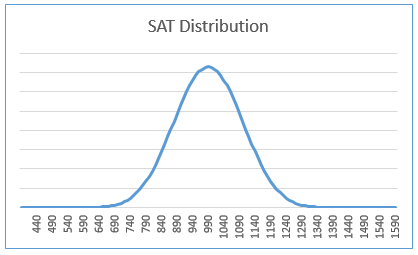
\includegraphics[width=\maxwidth{.95\linewidth}]{gfx/06-SATDistro}
	\caption{Normal Distribution}
	\label{fig06.01}
\end{figure}

SAT scores lie between $ 400 $ and $ 1600 $ as listed across the X-Axis and the number of students who earn each score is plotted. Since the most common score is $ 1000 $ that score is at the peak of the curve. Very few students scored above $ 1300 $ or below $ 650 $ and the curve is near the lower bound beyond those points. This illustrates a normal distribution where most scores are bunched near the center of the graph with only a few at either extreme.

The normal distribution is important because it permits researchers to use specific techniques to test a hypothesis about the sample. For example, perhaps a researcher hypothesized that the graduation rate at university ``A'' was higher than at university ``B'' because students' SAT scores were higher. Since SAT scores have a normal distribution, the researcher could use specific tests, like a t-test, to support or refute the hypothesis. However, if the data were not normally distributed then the researcher would need to use a different group of tests.

\subsection{Excess Kurtosis}
One way to mathematically describe a normal distribution is to calculate the length of the tails of a bell curve, and that is called its \gls{excesskurtosis}. For a normal distribution the excess kurtosis is $ 0.00 $, a positive excess kurtosis would indicate longer tails while a negative excess kurtosis would indicate shorter tails. Intuitively, many people believe the excess kurtosis represents the ``peaked-ness'' of the curve since longer tails would tend to lead to a more peaked graph; however, excess kurtosis is a measure of the data outliers, which would be only present in the tails of the graph; so excess kurtosis is not directly indicative of the the ``sharpness'' of the peak. It is difficult to categorically state that some level of excess kurtosis is good or bad. In some cases, data that form a graph with longer tails are desired but in other cases they would be a problem.

Following are three examples of excess kurtosis. Notice that as the excess kurtosis increases the tails become longer. 

\begin{figure}[H]
	\centering
	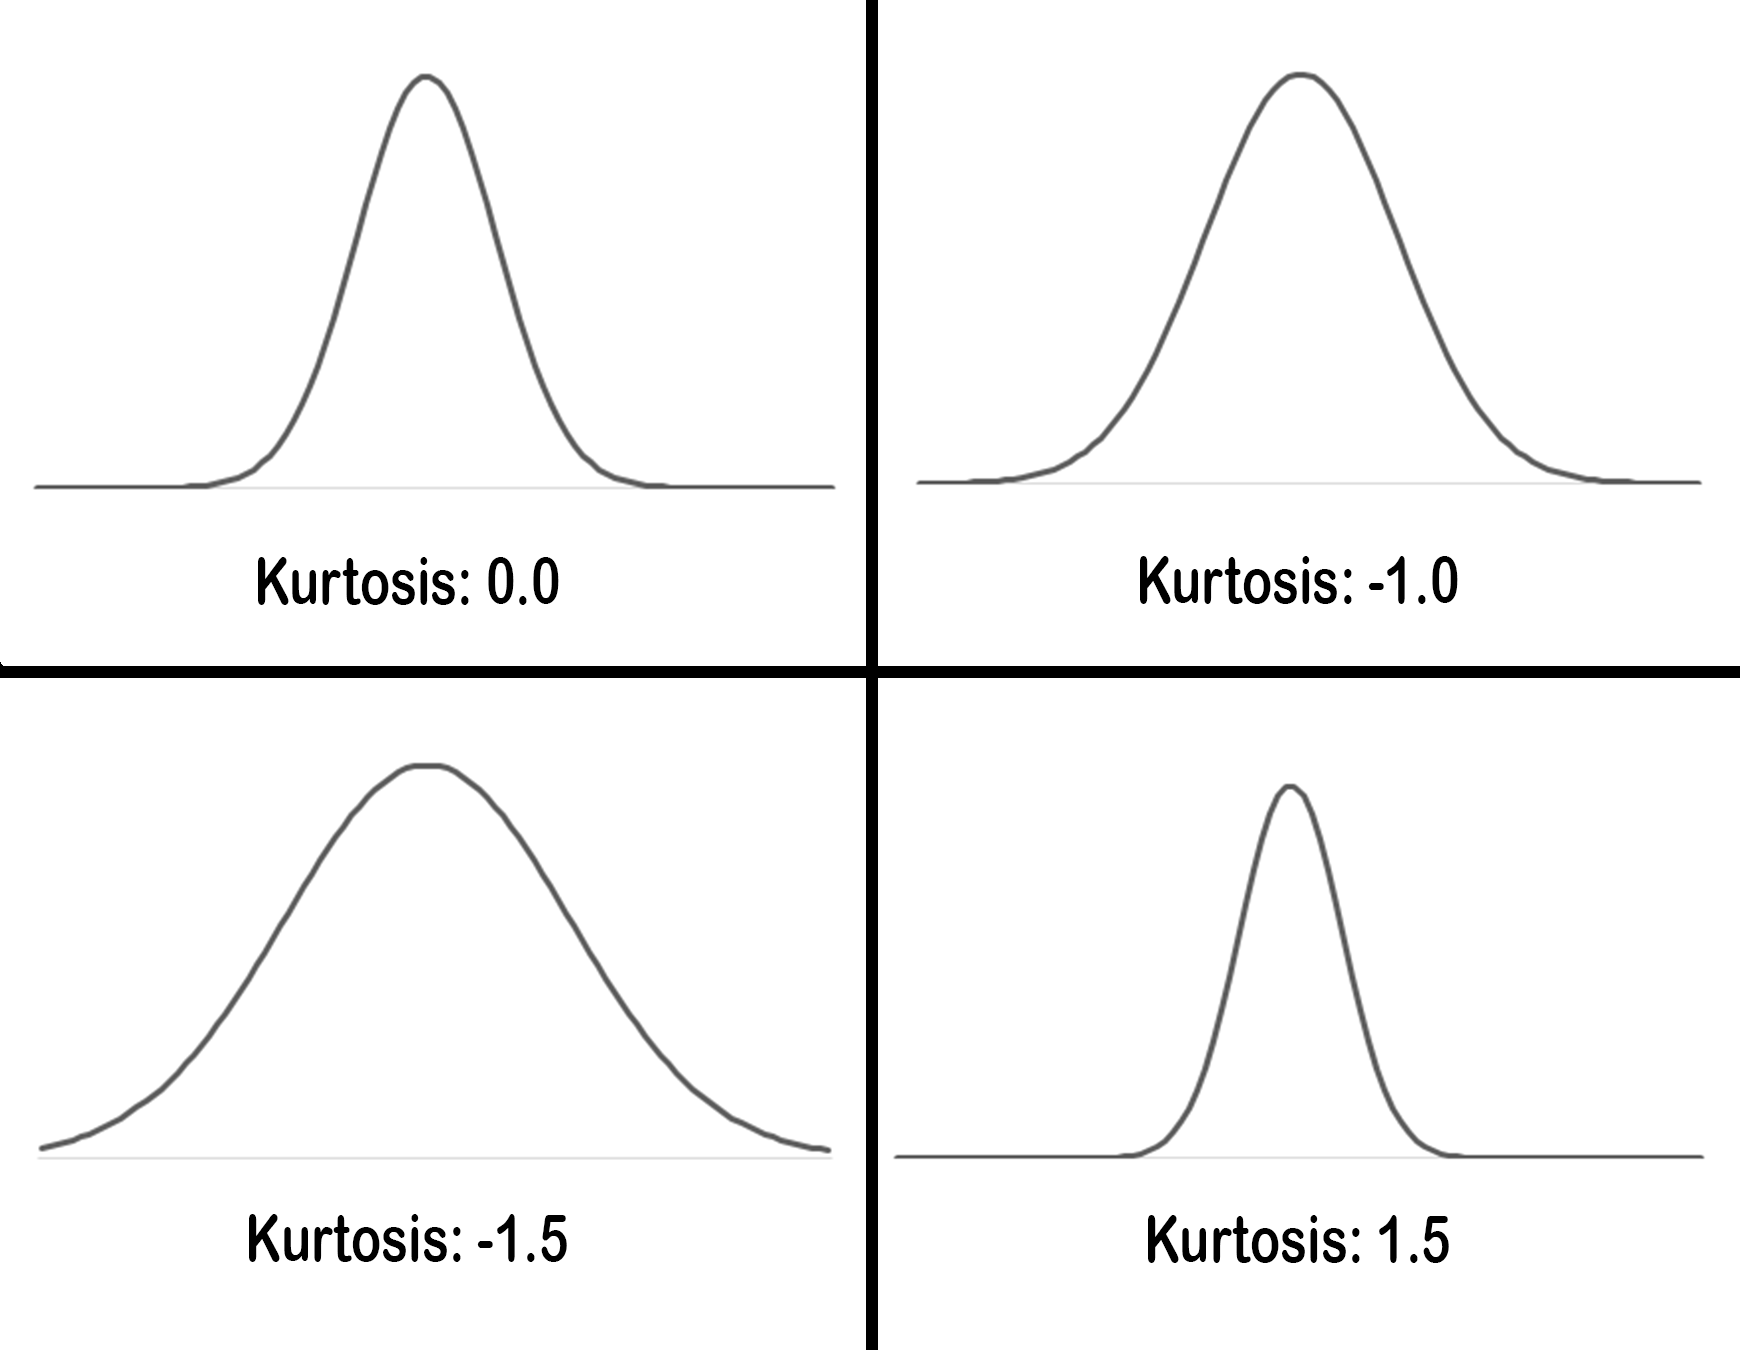
\includegraphics[width=\maxwidth{.95\linewidth}]{gfx/06-Kurtosis}
	\caption{Kurtosis in a Normal Distribution}
	\label{fig06.02}
\end{figure}

\subsection{Skew}
The second numerical measure of a normal distribution that is frequently reported is its \gls{skew}, which is a measure of the symmetry of the curve about the mean of the data. The normal distribution in Figure \ref{fig06.03} has a skew of $ 0.00 $. A positive skew indicates that the tail on the right side is longer, which means that there are several data points on the far right side of the graph ``pulling'' the tail out that direction. A negative skew indicates that the tail on the left side of the graph is longer. Following are three examples of skew:

\begin{figure}[H]
	\centering
	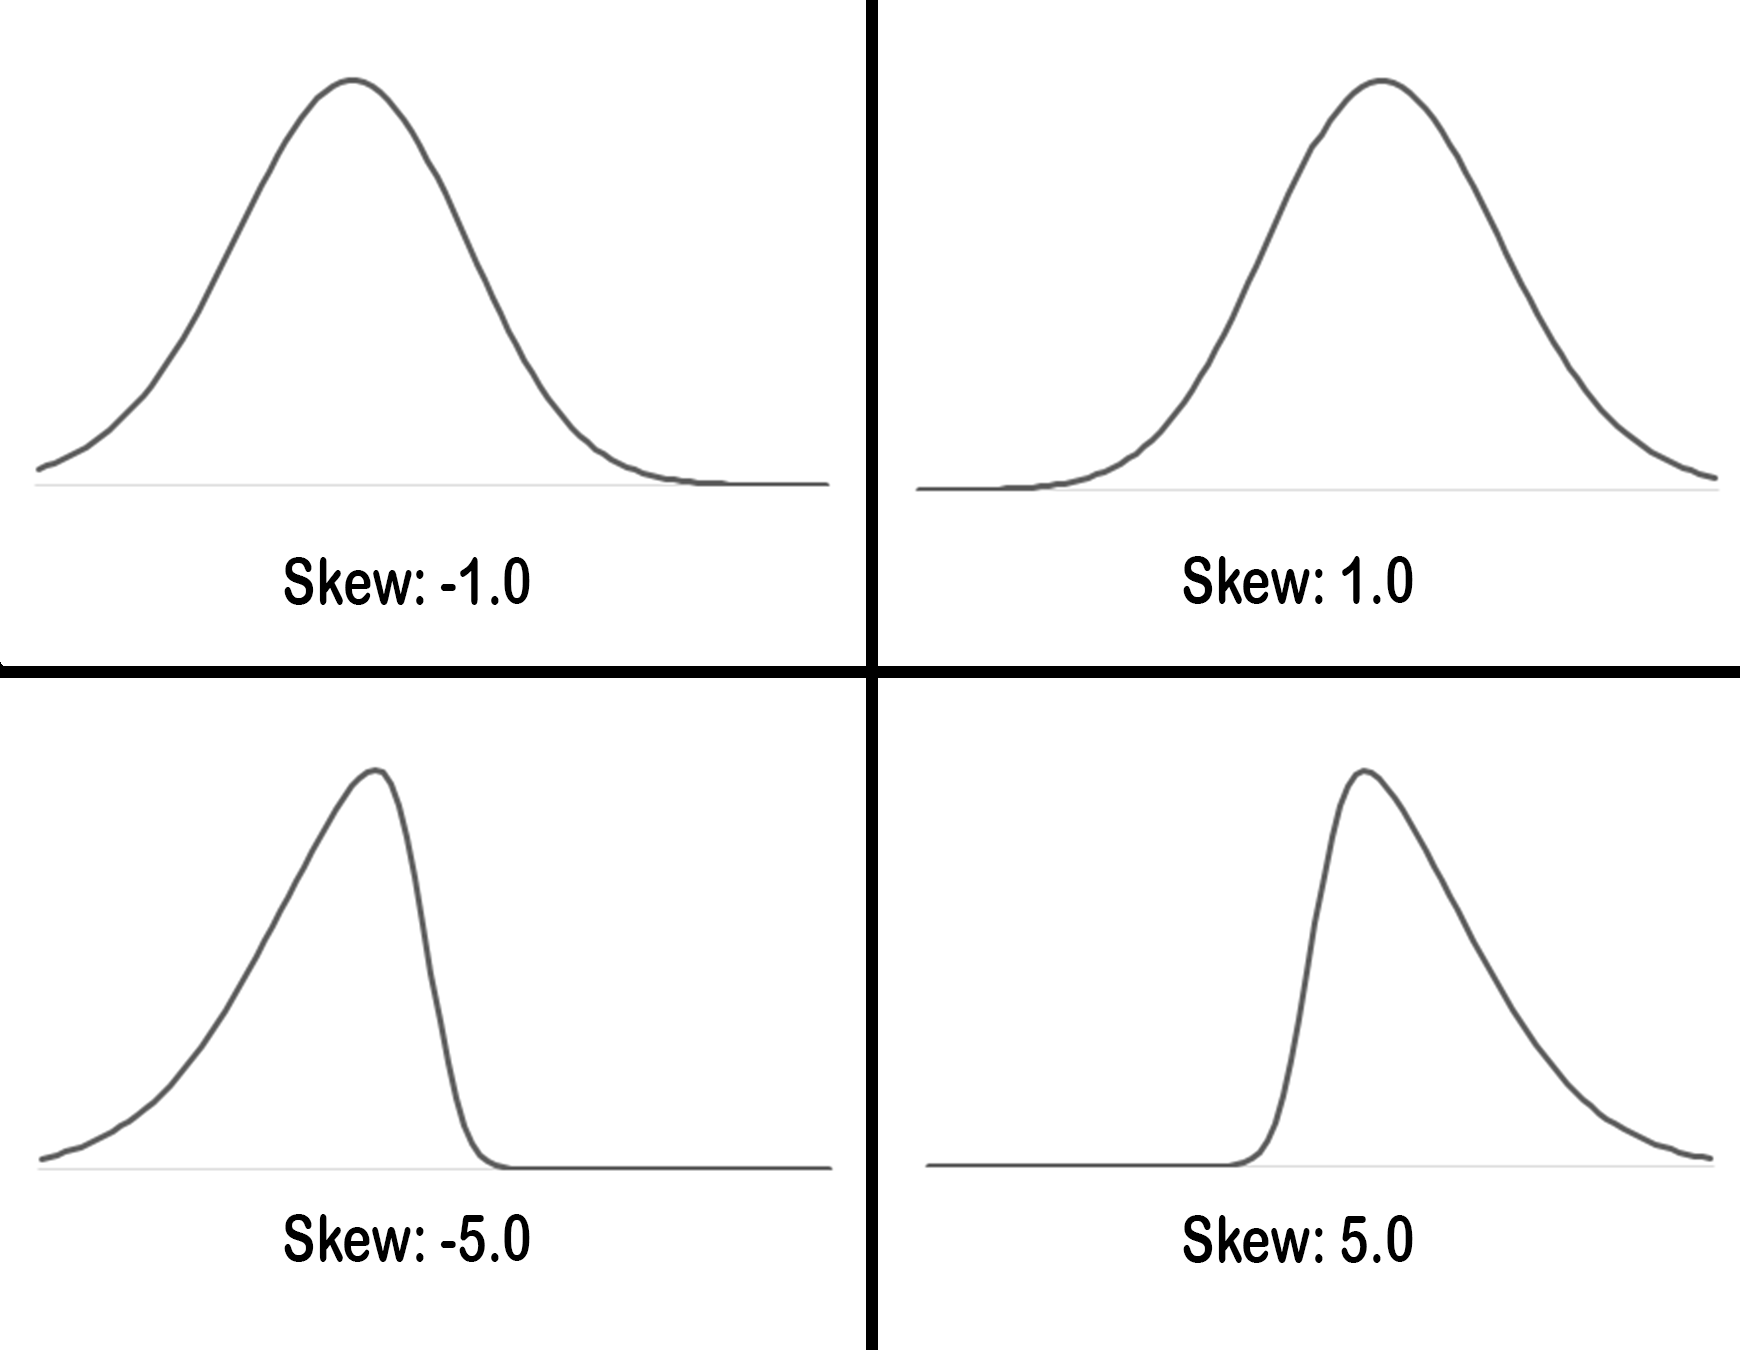
\includegraphics[width=\maxwidth{.95\linewidth}]{gfx/06-Skew}
	\caption{Skew in a Normal Distribution}
	\label{fig06.03}
\end{figure}

\section{Databases}

When a lot of data are gathered into a single location they are referred to as a \gls{database}. This is not a new concept. Fifty years ago a library would have a series of 3X5 cards that contained information about all of the books in the library (title, author, subject, etc.). Those cards were stored in a wooden cabinet called the ``card catalog'' and customers could find information about and the location of whatever book they wanted. Today, databases are often contained in electronic form on the internet where they can be accessed from customers' home computers, tablets, or even phones.

Data in a database is typically stored in tables that resemble spreadsheets, that is, rows and columns where each row is one record (or observation) about some phenomenon and each column is one descriptor of that record. For example, a database that contains information about the people who work at a company would be organized such that each row contained data about just one person and each column would contain a single aspect of that person's employment, like name, employee number, date of birth, etc.\footnote{Of course, databases are much more complex than described in this paragraph but this is not a database text so the simple explanation offered is adequate for this context.} A database is designed to deliver answers to questions through a lookup process so, for example, if the CEO of a company wanted to know the birth date for someone in the accounting department that data could be easily found. 

One common problem with any database is ``dirty data.'' These are data that contain errors or are missing. For example, it is easy for a data entry clerk to enter something like ``1000000'' instead of ``100000'' (count the zeros) for a person's salary and create an ``outlier'' in the data. Another common problem are missing data. For example, if employees are asked to update their personal information but someone could not remember their ZIP code then they would simply leave that field blank.

Dirty data makes it difficult to analyze the database. For example, if a researcher wanted to report the median salary for the workers in a factory but ten percent of the salaries were missing from the database then the median would not be accurate. There are several methods statisticians use to mitigate the problems caused by dirty data but those are beyond the scope of this text. 

\subsection{Public Databases}

There are hundreds of publicly available databases that can be used for research. As one example, the United States Census Bureau maintains a huge database that contains information about the people of the United States.\footnote{The US Census Bureau's website is at \url{https://www.census.gov/}.} The data at that site is freely available to anyone who wants to use it, and the site is organized so information is fairly quick and easy to find. As an example, it is not difficult to discover that among adults in the United States, 29\% have a high school diploma, 20\% have a Bachelor's degree, 8\% have a Master's degree, 1.7\% have a Doctoral degree, and the rest fall elsewhere on the education spectrum. The US Census Bureau has more advanced tools available that permit researchers to focus on a single county or even smaller region.

When using a public database, a researcher must be concerned with bias. Since the researcher did not gather the data first-hand it is possible that the data are biased. For example, if the database includes people's attitude towards work how is the researcher going to know if the data gathered was from a well-designed, neutral survey or if it was just gathered using some sort of convenience sample? In general, databases found at governmental websites (with urls that end with .gov) or education websites (with urls that end with .edu) would more likely be bias-free while databases from .com sites would need to have extra attention paid to bias.

Sometimes, students will find a website with a list of links to journal articles or chapters from books. While these are valuable resources for a researcher, they are not the same as a database that contains raw data from a survey, experiment, or other activity. Journal articles provide good information for a literature review but would not be appropriate for an online database source.

\subsection{Using Public Databases}

As an example of using a public database, imagine that the CEO of ``BASVFOODS'' is interested in opening a neighborhood market in a small town they have never serviced before. In order to gather information about that location it is possible to use US Census Bureau data to find out things like the median household size, income, and education level. The CEO could then compare that data with similar data from a town that has a successful store to help inform a decision to open a new store.

\section{Statistical Test Selection}

Once the data are gathered it is important to run some statistical processes to see if the data contains anything of interest. While there are hundreds of tests that can be used, here is a bit of information about the most common tests.

When researchers are determining what type of statistical test to use they must consider the goal of the analysis and the type of data being analyzed. To begin to determine what statistical tests are appropriate, start by classifying the variables being evaluated. 

\begin{itemize}
	\item Quantitative variables are numeric and are found through measurement or counting. Continuous data can be any value, including fractions or decimals, like a person's height or the length of time it takes to complete some task. Discrete data are integers normally found by counting, like the number of people at an event or the age of a respondent.
	\item Qualitative variables are non-numeric and are found by people checking boxes on a survey. Ordinal data have some implied order, like a student's class (senior, junior, etc.) or the level of agreement with a statement. Nominal data have no order, like a respondent's gender.
\end{itemize}

\begin{figure}[H]
	\centering

	\forestset{qtree/.style={for tree={parent anchor=south, 
			child anchor=north,
			align=center,
			inner sep=3pt,
			draw}}}
		
	\begin{forest}, baseline, qtree
		[Variable, fill=purple!40!white
			[{Quantitative\\(Measure or count)}, fill=cyan!40!white
				[{Continuous\\(Any value)}, fill=cyan!20!white]
				[{Discrete\\(Integers)}, fill=cyan!20!white]
			]
			[{Qualitative\\(Tick boxes)}, fill=pink!60!white
				[{Ordinal\\(Ordered)}, fill=pink!40!white]
				[{Nominal\\(No order)}, fill=pink!40!white]
			]
		]
	\end{forest}

	\caption{Classifying Variables}
	\label{fig06.08}
\end{figure}

\subsection{Summary Statistics}

One of the easiest type of analysis to complete is determining the center and spread of a data set. This analysis is also one of the first that research readers expect to find. Here is a guide for what sort of central measure and spread to report.

\begin{itemize}
	\item For normally distributed data use the mean and standard deviation.
	\item For skewed data use the median and Interquartile Range (IQR).
	\item For ordinal data use the median and Interquartile Range (IQR).
	\item For nominal data use the mode as a central measure but there is no spread.
\end{itemize}

\begin{figure}[H]
	\centering
	
	\forestset{qtree/.style={for tree={parent anchor=south, 
				child anchor=north,
				align=center,
				inner sep=3pt,
				draw}}}
	
	\begin{forest}, baseline, qtree
		[Which summary and spread, fill=brown!40!white
			[{Quantitative}, fill=orange!40!white
				[{Normal Distribution\\(Mean\\Standard deviation)}, fill=orange!20!white]
				[{Skewed Data\\(Median\\IQR)}, fill=orange!20!white]
			]
			[{Qualitative}, fill=yellow!60!white
				[{Ordinal\\(Median\\IQR)}, fill=yellow!40!white]
				[{Nominal\\(Mode\\No range)}, fill=yellow!40!white]
			]
		]
	\end{forest}
	
	\caption{Central Measure and Spread}
	\label{fig06.09}
\end{figure}

\subsection{Parametric vs. Nonparametric Tests}

Normally, a researcher posits a hypothesis and then conducts research to either support or refute that hypothesis. The type of hypothesis test needed depends on the type of the variables being tested. There are two broad categories of variables in a hypothesis test: independent and dependent.

\begin{itemize}
	\item Independent variables (explanatory variables) are those that cause something to happen; they explain why some outcome was observed. For example, if the hypothesis is that women spend more on groceries than men then the independent variable is the sex of the shopper. If the hypothesis is that old people are more dangerous drivers than young people then the independent variable is the age of the driver.
	\item Dependent variables (outcome variables) are those that are the outcome for whatever is happening. For example, if the hypothesis is that women spend more on groceries than men then the dependent variable is amount of money spent. If the hypothesis is that old people are more dangerous drivers than young people then the dependent variable is the number of accidents reported.
\end{itemize}

The chart in Figure \ref{fig06.10} is used to determine if the hypothesis test should be parametric or nonparametric.

\begin{itemize}
	\item Parametric tests assume that the data follows a particular distribution, usually normally distributed. Parametric tests are more powerful than nonparametric tests and are more likely to detect true differences or relationships that exist.
	\item Nonparametric tests are used when the dependent variable is not normally distributed; that is, the data are skewed or are nominal. Nonparametric techniques are usually based on ranks or signs rather than the actual data and are usually less powerful than parametric tests.
\end{itemize}

\begin{figure}[H]
	\centering
	
	\forestset{qtree/.style={for tree={parent anchor=south, 
				child anchor=north,
				align=center,
				inner sep=3pt,
				draw}}}
	
	\begin{forest}, baseline, qtree
		[Dependent Variable, fill=green!40!white
		[{Quantitative}, fill=teal!40!white
		[{Normal Distribution\\(Parametric)}, fill=teal!20!white]
		[{Skewed Data\\(Nonparametric)}, fill=teal!20!white]
		]
		[{Qualitative}, fill=lime!60!white
		[{Ordinal\\(Nonparametric)}, fill=lime!40!white]
		[{Nominal\\(Chi-square)}, fill=lime!40!white]
		]
		]
	\end{forest}
	
	\caption{Parametric vs. Nonparametric Selection}
	\label{fig06.10}
\end{figure}

\subsection{Hypothesis Test Selection}

Table \ref{tab06.07} lists the hypothesis tests that are commonly used to compare the averages of two or more groups.

\begin{table}[H]
	\centering
	\definecolor{ltgray}{gray}{0.95} % this is a light gray
	\rowcolors{1}{}{ltgray} % zebra striping background
	\begin{tabularx}{0.95\linewidth}{p{0.25\linewidth}
			p{0.15\linewidth}
			p{0.15\linewidth}
			p{0.15\linewidth}
			p{0.15\linewidth}
		}
		\toprule
		\textbf{Comparing} & 
			\textbf{Dep Var} & 
			\textbf{Ind Var} &
			\textbf{Para} & 
			\textbf{NonPara} \\
		\midrule
		2 independent \newline groups & Quant & Binary & Indep t-test & Mann-Whitney \\
		3+ independent \newline groups & Quant & Nom & ANOVA & Kruskal-Wallis \\
		2 matched \newline groups & Quant & Time & Paired t-test & Wilcoxon \\	
		3+ measures \newline same subj & Quant & Time & Rep ANOVA & Friedman \\		

		\bottomrule
	\end{tabularx}
	\caption{Tests to Compare Two or More Samples}
	\label{tab06.07}
\end{table}


Table \ref{tab06.08} lists the hypothesis tests that are commonly used to find any associations relationships (correlations) between two groups.

\begin{table}[H]
	\centering
	\definecolor{ltgray}{gray}{0.95} % this is a light gray
	\rowcolors{1}{}{ltgray} % zebra striping background
	\begin{tabularx}{0.95\linewidth}{p{0.25\linewidth}
			p{0.15\linewidth}
			p{0.15\linewidth}
			p{0.15\linewidth}
			p{0.15\linewidth}
		}
		\toprule
		\textbf{Comparing} & 
		\textbf{Dep Var} & 
		\textbf{Ind Var} &
		\textbf{Para} & 
		\textbf{NonPara} \\
		\midrule
		2 Continuous & Quant & Quant & Pearson's r & Spearman's rho \\
		Prediction & Quant & Any & Regression & None \\
		Prediction & Nominal & Any & Log \newline regression & None \\	
		2 Qual vars & Qual & Qual & None & Chi-square \\		
		
		\bottomrule
	\end{tabularx}
	\caption{Tests to Association Between Two Samples}
	\label{tab06.08}
\end{table}


\section{Statistical Test Sampler}

\subsection{Central Measures}

\subsection{Dispersion}

\subsection{Frequency Tables}

\subsection{Correlation}

\subsection{Parametric Hypothesis Tests}

\subsection{Nonparametric Hypothesis Tests}

\subsection{Data Mining}

\subsubsection{K-Means Clusters}

\subsubsection{Decision Tree}

\begin{figure}[H]
	\centering
	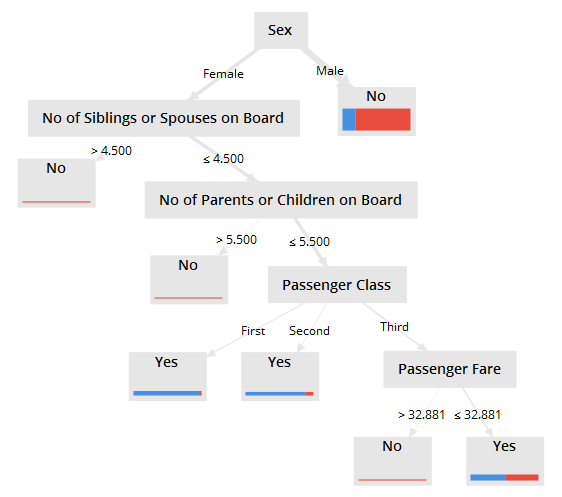
\includegraphics[width=\maxwidth{.95\linewidth}]{gfx/06-DecisionTree}
	\caption{Decision Tree}
	\label{fig06.05}
\end{figure}




\subsubsection{Market Basket}

\begin{figure}[H]
	\centering
	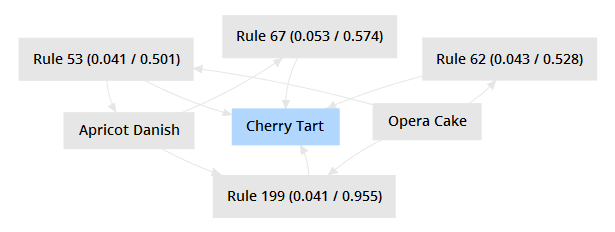
\includegraphics[width=\maxwidth{.95\linewidth}]{gfx/06-MarketBasketGraph}
	\caption{Market Basket Graph}
	\label{fig06.06}
\end{figure}


\begin{figure}[H]
	\centering
	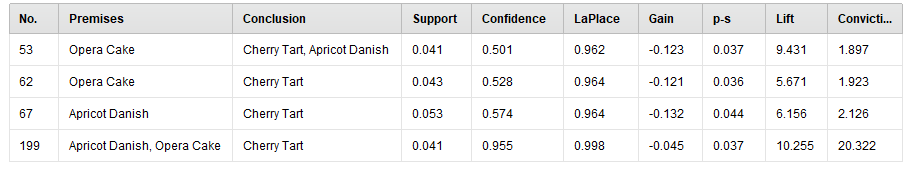
\includegraphics[width=\maxwidth{.95\linewidth}]{gfx/06-MarketBasketRules}
	\caption{Market Basket Rules}
	\label{fig06.07}
\end{figure}


\section{Summary}\label{ch06:summary}

Figure \ref{fig06.04} illustrates the relationship between the various types of data and the rating scales commonly used to work with those data types. Researchers with a positivism philosophy tend to use parametric statistical analysis and gather interval and ratio data. Researchers with an interpretivism philosophy tend to use nonparametric statistical analysis and gather nominal and ordinal data. Nominal data are typically gathered with binary and semantic difference rating scales while ordinal data are typically gathered with Likert and Guttman rating scales.

\begin{figure}[H]
	\centering
	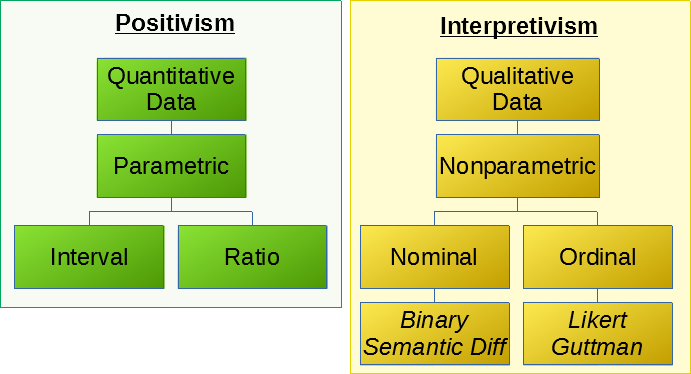
\includegraphics[width=\maxwidth{.95\linewidth}]{gfx/06-DataTypes}
	\caption{Data types}
	\label{fig06.04}
\end{figure}
 
%%*****************************************
\chapter{Sampling}\label{07:sampling}
%*****************************************
%TODO Status: Pre-draft

\begin{wrapfigure}{O}{0.4\textwidth}
	\label{07:fig01} 
	\centering
	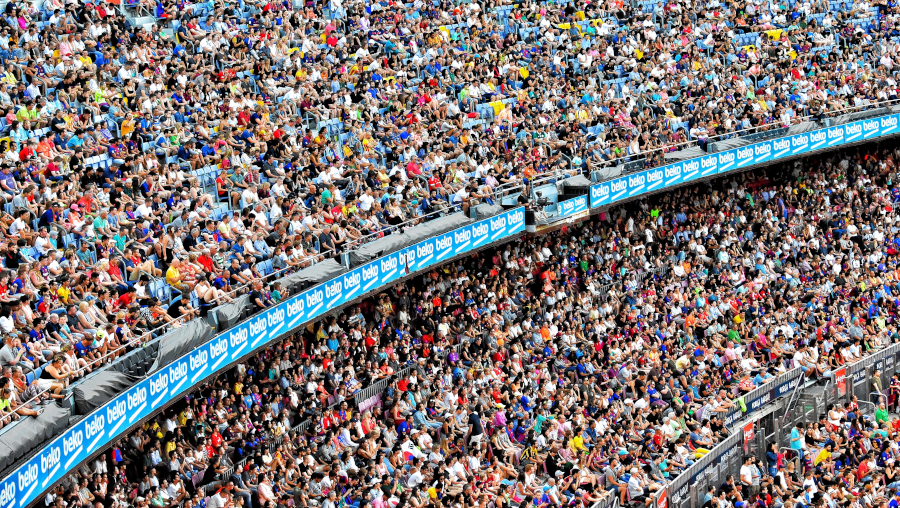
\includegraphics[width=0.4\textwidth]{gfx/07-01} 
\end{wrapfigure}
Imagine that a research team undertakes a project to determine the number of t-shirts to order for an upcoming promotion in a large stadium. The question that the stadium owner needs answered is how many small/medium/large t-shirts should be ordered. To figure that out, the researchers decide to conduct a survey of the fans a few weeks before the promotion and ask them what size t-shirt they would prefer. So, how many fans should they survey? They could ask every fan in the stadium if they hired enough poll-takers, but that would be expensive and wasteful. Perhaps it is enough to ask $ 10\% $ of the crowd -- maybe just $ 1\% $. Once the researchers figure out how many people to survey, then they need to figure out how to select those people. Do they select everyone in a specific section? Do they ask the first 100 people who come through a specific gate? These are questions that concern sampling and whatever decisions the researchers make concerning the stadium crowd may profoundly change the data that are collected, and not necessarily for the best. This chapter concerns sampling and offers information about how to determine a sample size and what techniques can be used to reduce bias in the sample.
\blfootnote{Photo by Ekansh Saxena on Unsplash}

\section{Introduction}

Business and marketing research generally concerns inferring patterns of behaviors within specific populations where a ``population'' is a cluster of people, events, things, or other phenomena of interest. Unfortunately, populations may be rather large and vaguely defined, such as ``the American people,'' or ``grocery stores in the United States.'' Even those populations that are not so vague can also be too large to study directly, like all shoppers over the age of $ 18 $ within a specific region. Normally, it is not feasible to study an entire population because of cost constraints so a representative sample is selected from the population for observation and analysis. 

A sample is a small subset of the population from which data are gathered in order to make statistical inferences about the entire population. Sampling strategies are designed to allow researchers to make claims about populations that are much larger than they actually sample with a fair amount of confidence. It is extremely important for researchers to choose a sample that is truly representative of the population so the inferences derived can be generalized back to the entire population. Improper and biased sampling is the primary reason for the often divergent and erroneous inferences reported in opinion polls conducted by different groups prior to every United States Presidential election.

The sampling process involves several stages. 

\begin{enumerate}
	\item Defining the target population. A population can be defined as all people or items (unit of analysis) with the characteristic of interest. The unit of analysis may be a person, group, organization, country, object, or any other entity about which scientific inferences can be drawn. Sometimes the population is obvious. For example, if a manufacturer wants to determine whether finished goods manufactured on a particular production line meets certain quality requirements then the population consists of the entire set of finished goods manufactured on that line. At other times the target population may be a little harder to understand. If the research project is to identify the primary motivators of shopping behavior among high school students then the target population may be high school students, store managers who are selling products to those students, or even the product manufacturers who design the packaging. 

	\item Determine the sampling frame. This is an accessible section of the target population (often a list with contact information) from which a sample can be drawn. If the target population is ``professional employees'' then the sampling frame would likely be the professional employees at a local company since it would not be possible to access all professional employees around the world. If the target population is ``business organizations'' then the Fortune $ 500 $ list may be an acceptable sampling frame.

	Note that sampling frames may not be representative of the population at large so inferences derived by that sample may not be generalizable to the population. For instance, if the target population is the employees of small businesses and the sampling frame is employees at automotive tire companies in the American Midwest then findings from that group may not be generalizable to the American workforce at large, let alone the global workplace. Similarly, the Fortune $ 500 $ list includes the $ 500 $ largest American enterprises, which is not representative of American firms in general, most of which are medium and small-sized firms. Also note that the population from which a sample is drawn may not necessarily be the same as the population about which the research is targeted. For example, if a researcher wants to the success rate of a new ``quit smoking'' program, then the target population is the universe of smokers who had access to this program, which may be an unknown population. Hence, the researcher may sample patients arriving at a local medical facility for smoking cessation treatment, some of whom may not have had exposure to this particular ``quit smoking'' program, in which case, the sampling frame does not correspond to the population of interest.

	\item Select a sample. Once the sampling frame is defined the actual sample must be drawn using a well-defined technique. Sampling techniques can be grouped into two categories: probability (or random) sampling and non-probability sampling. Probability sampling is important if the results are to be generalized but there may be unique circumstances where non-probability sampling can also be justified.

\end{enumerate}

As an example of this process, consider Figure \ref{07:fig11}\footnote{Photo of the population by not brittany shh pls on Unsplash. Photo of the list by Sophia Baboolal on Unsplash. Photo of the two men by rawpixel on Unsplash}. Imagine that a researcher intends to conduct some sort of project where the intent is to draw some conclusions about professional workers around the world. That population would be much too large to survey directly, so a sampling frame would be created of, perhaps, the professional workers at two or three local companies. From that frame, specific workers would be selected for observation.

\begin{figure}[H]
	\centering
	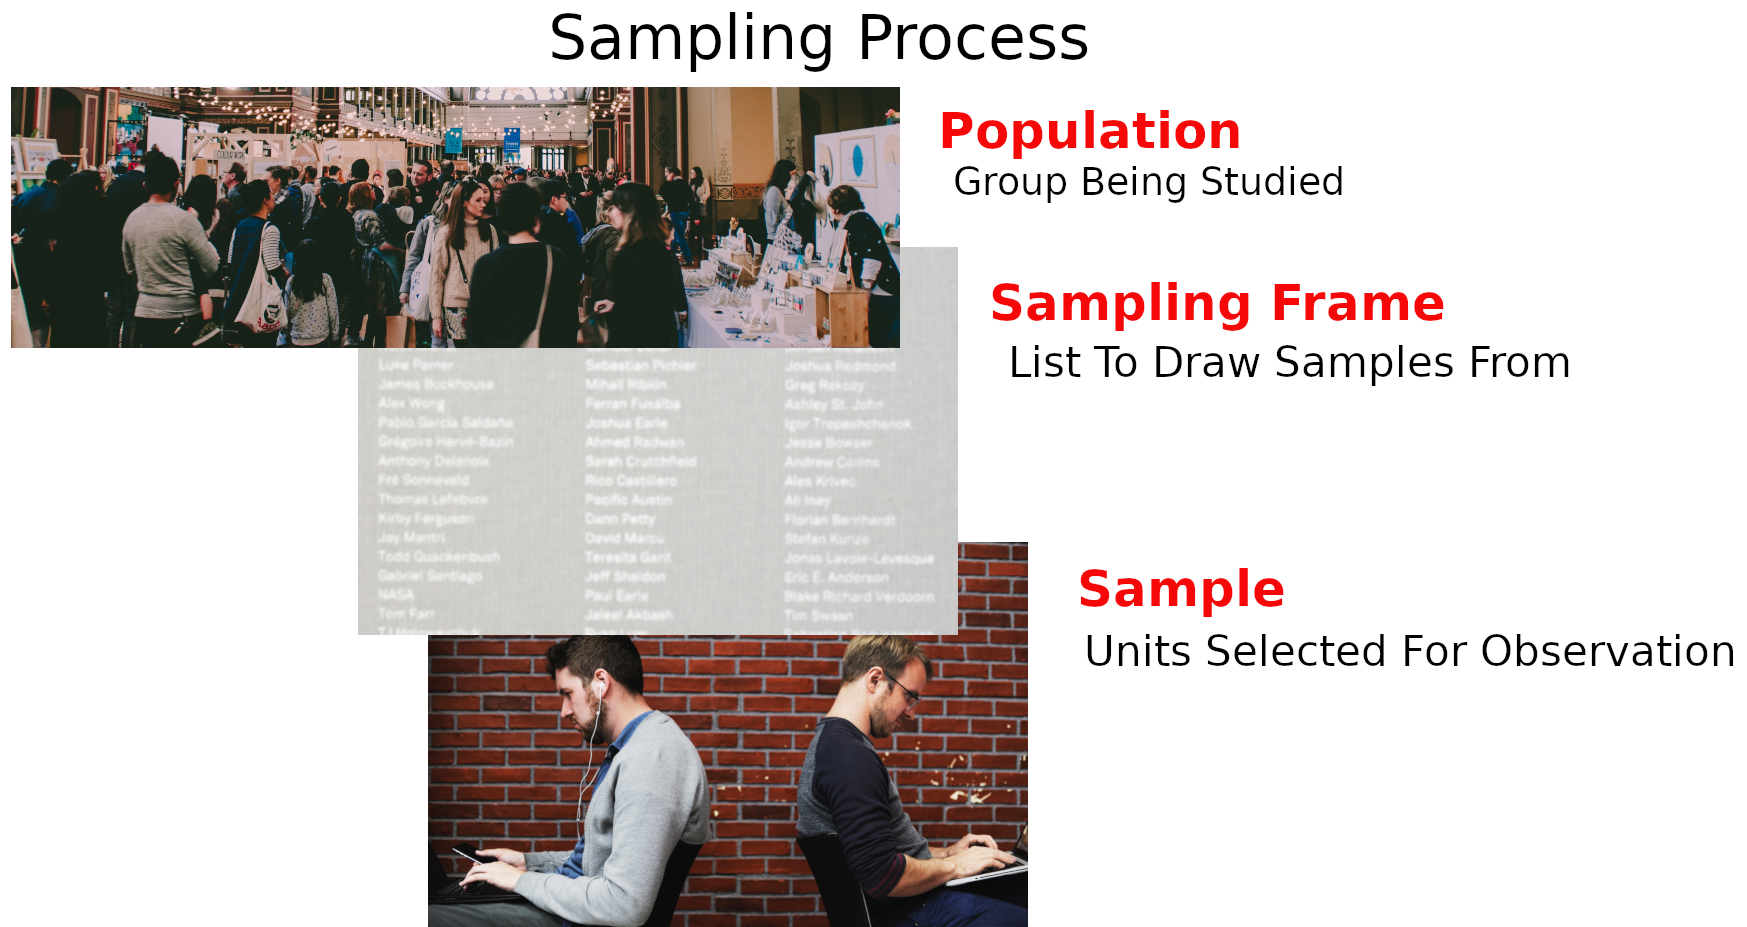
\includegraphics[width=\maxwidth{.95\linewidth}]{gfx/07-11}
	\caption{Sampling Process Visualized}
	\label{07:fig11}
\end{figure}

Both qualitative and quantitative researchers use sampling techniques but because the goals of qualitative and quantitative research differ the sampling procedures employed are also different.

\section{Sampling in Quantitative Research}

Quantitative researchers are often interested in being able to make generalizations about populations that are larger than their study samples and rely on \textit{probability sampling}. Probability sampling is a technique in which every unit in the population has a chance (non-zero probability) of being selected to be sampled and this chance can be accurately determined. It is important that every element in the sample frame has a known chance to be sampled because that makes the sample representative of the entire population. If, for example, a researcher is investigating something about the differences between men and women shoppers then it would be important that the sample contained both men and women in about the same proportions as in the entire population. This is a bit of an over-simplification but it points out the importance of a representative sample. Obtaining a representative sample is also important because a key goal of studies that rely on probability samples is generalizability. In fact, generalizability is perhaps the key feature that distinguishes probability samples from non-probability samples. Generalizability refers to the idea that the results will indicate something about the entire population.

One goal for a parametric sample is that it forms a normal distribution and has negligible skew and excess kurtosis \footnote{See Chapter 6 for a definition of skew and excess kurtosis}. Statistics that are generated from the sample, such as the mean or standard deviation, are unbiased estimates of population parameters as long as the samples are selected properly. Therefore, statistical analysis of the sample can be reasonably applied to the entire population. All probability sampling has two attributes in common: 1) every unit in the population has a known non-zero probability of being sampled, and 2) the sampling procedure involves random selection. The different types of probability sampling techniques include the following

\textbf{Simple Random Sampling} In this technique, all possible subsets of a population (more accurately, of the sampling frame) have an equal probability of being selected, making the sample an unbiased estimate of the population. 

Simple random sampling involves randomly selecting respondents from a sampling frame, usually employing a table of random numbers\footnote{A table of random numbers can be generated at \url{http://stattrek.com/Tables/Random.aspx}.} or a computerized random number generator. For instance, to randomly select $ 200 $ firms to survey from a list of $ 1000 $ firms the list could be entered into a spreadsheet program like Excel then the ``random'' function could be used to generate a random number for each of the $ 1000 $ firms. Next, the list is sorted by the random number and the first $ 200 $ firms on that sorted list would be selected. This is the simplest of all probability sampling techniques and that simplicity is also its greatest strength. Because the sampling frame is not subdivided or partitioned, the sample is unbiased and the inferences are the most generalizable when compared to other probability sampling techniques.

Figure \ref{07:fig02} illustrates simple random sampling. A few individuals in the entire population are selected (circled) at random for the study.

\begin{figure}[H]
	\centering
	
\includegraphics[width=\maxwidth{.35\linewidth}]{gfx/07-02}
	\caption{Simple Random Sampling}
	\label{07:fig02}
\end{figure}

\textbf{Systematic Sampling} In this technique, the sampling frame is ordered according to some criteria and then elements are selected at regular intervals through that ordered list. Systematic sampling involves a random start and then proceeds with the selection of every \textit{kth} element from that point onwards. The value of \textit{k} is easily calculated by $ k = N/n $, where \textit{k} (the sampling ratio) is calculated by dividing the size of the sampling frame, \textit{N}, by the desired number of samples, \textit{n}. It is important that the starting point is not automatically the first item in the list, but is instead randomly chosen from within the first \textit{k} elements on the list. Using the previous example of selecting $ 200 $ firms from a list of $ 1000 $, \textit{k} is equal to $ 5 $ ($ k = 1000/200 $). The list of $ 1000 $ firms would be sorted in increasing (or decreasing) order by some size-related criterion, like employee count or annual revenues. Then, one of the first five (the value of \textit{k}) firms on the list would be randomly selected and every fifth firm after that. This process ensures that there is no over-representation of large or small firms in the sample but, rather, that firms of all sizes are generally uniformly represented. In other words, the sample is representative of the population, at least on the basis of the sorting criterion.
	
There is one clear instance in which systematic sampling should be avoided. If the sampling frame has a pattern then bias can be introduced with a systemic sampling strategy. This is sometimes referred to as the problem of periodicity, which is the tendency for a pattern to occur at regular intervals. Imagine, for example, that a researcher wanted to observe how people use the outdoor spaces on a college campus. Perhaps the researcher selects ``random'' dates in the month of September to make observations but due to the way the weekdays cycle it is possible (in fact, likely) that all observations will be on the same day of the week. When working with patterned data it is best to not use systematic sampling.

Figure \ref{07:fig03} illustrates systematic sampling. In this case, $ k = 5 $ so every fifth person is chosen. At random, person three was chosen to start the pattern and then every fifth person after that is chosen.

\begin{figure}[H]
	\centering
	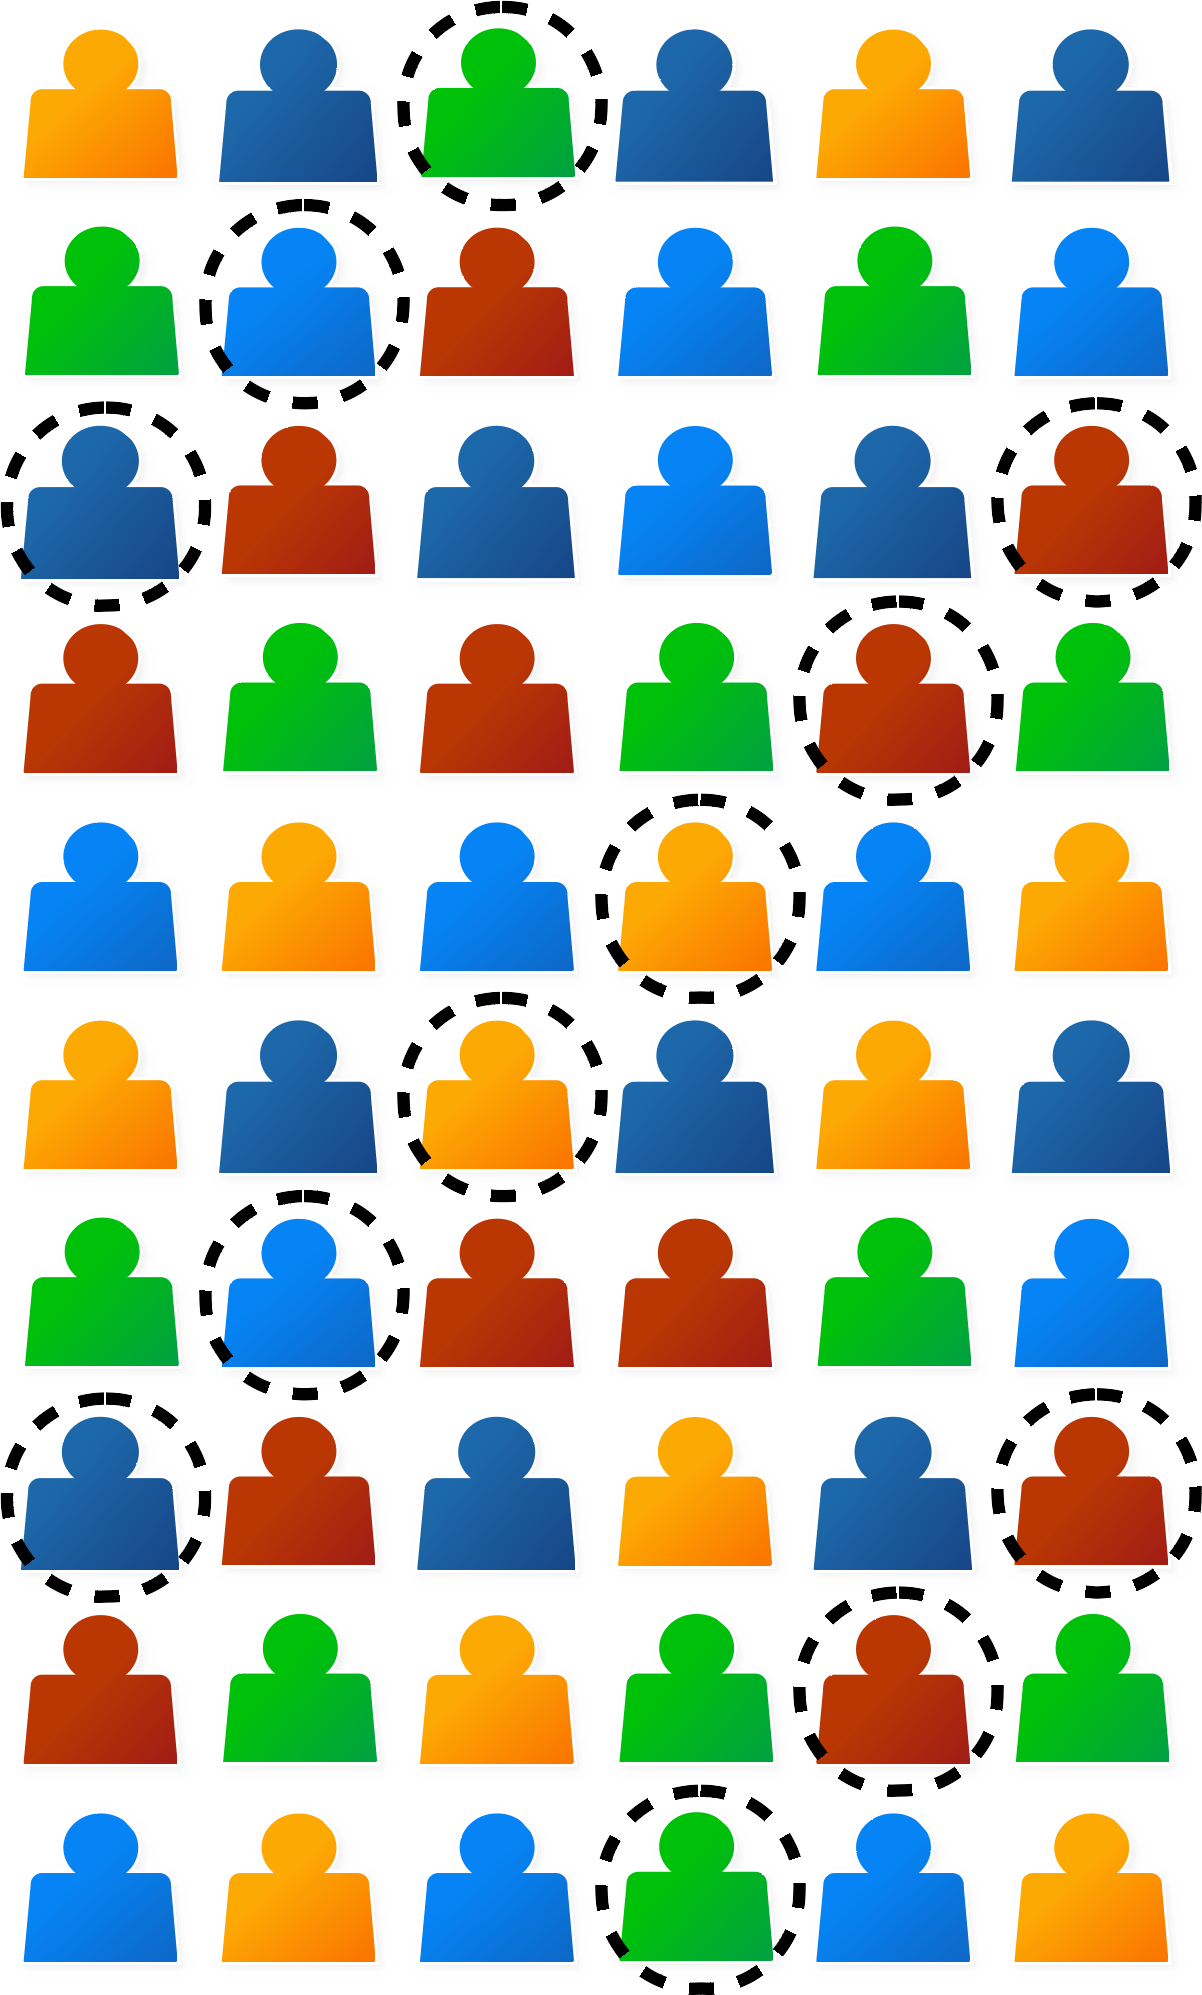
\includegraphics[width=\maxwidth{.35\linewidth}]{gfx/07-03}
	\caption{Systematic Sampling}
	\label{07:fig03}
\end{figure}

\textbf{Stratified Sampling} In stratified sampling, the sampling frame is divided into homogeneous and non-overlapping subgroups, called ``strata,'' and a simple random sample is drawn from each subgroup. Using the previous example of selecting $ 200 $ firms from a list of $ 1000 $, the firms could be categorized by size, perhaps ``large'' (more than $ 500 $ employees), ``medium'' ($ 50 - 500 $ employees), and ``small'' (fewer than $ 50 $ employees). Then, $ 67 $ firms would be randomly selected from each subgroup to create a sample of $ 200 $ firms. However, since there are many more small firms in a sampling frame than large firms, having an equal number of small, medium, and large firms will make the sample less representative of the population (in this case, biased in favor of large firms that are fewer in number in the target population). This is called non-proportional stratified sampling because the proportion of sample within each subgroup does not reflect the proportions in the sampling frame (or the population of interest), and the smaller subgroup (large-sized firms) is oversampled. 
	
An alternative technique is to select subgroup samples in proportion to their numbers in the population. For instance, if there are $ 100 $ ``large'' firms, $ 300 $ ``medium'' firms, and $ 600 $ ``small'' firms, then $ 20 $ should be selected from the ``large'' group, $ 60 $ from the ``medium'' group and $ 120 $ from the ``small'' group in order to maintain the correct proportion of firms. This technique is called \textit{proportional stratified sampling}. Note that the non-proportional approach is particularly effective in representing subgroups with fewer elements, such as large-sized firms in this example, but each subgroup's results must be weighted by its proportion in the population.

Figure \ref{07:fig04} illustrates stratified sampling. The population is divided into five subgroups and three elements were chosen from each subgroup. This would be an example of non-proportional stratified sampling since the same number are selected from each subgroup.

\begin{figure}[H]
	\centering
	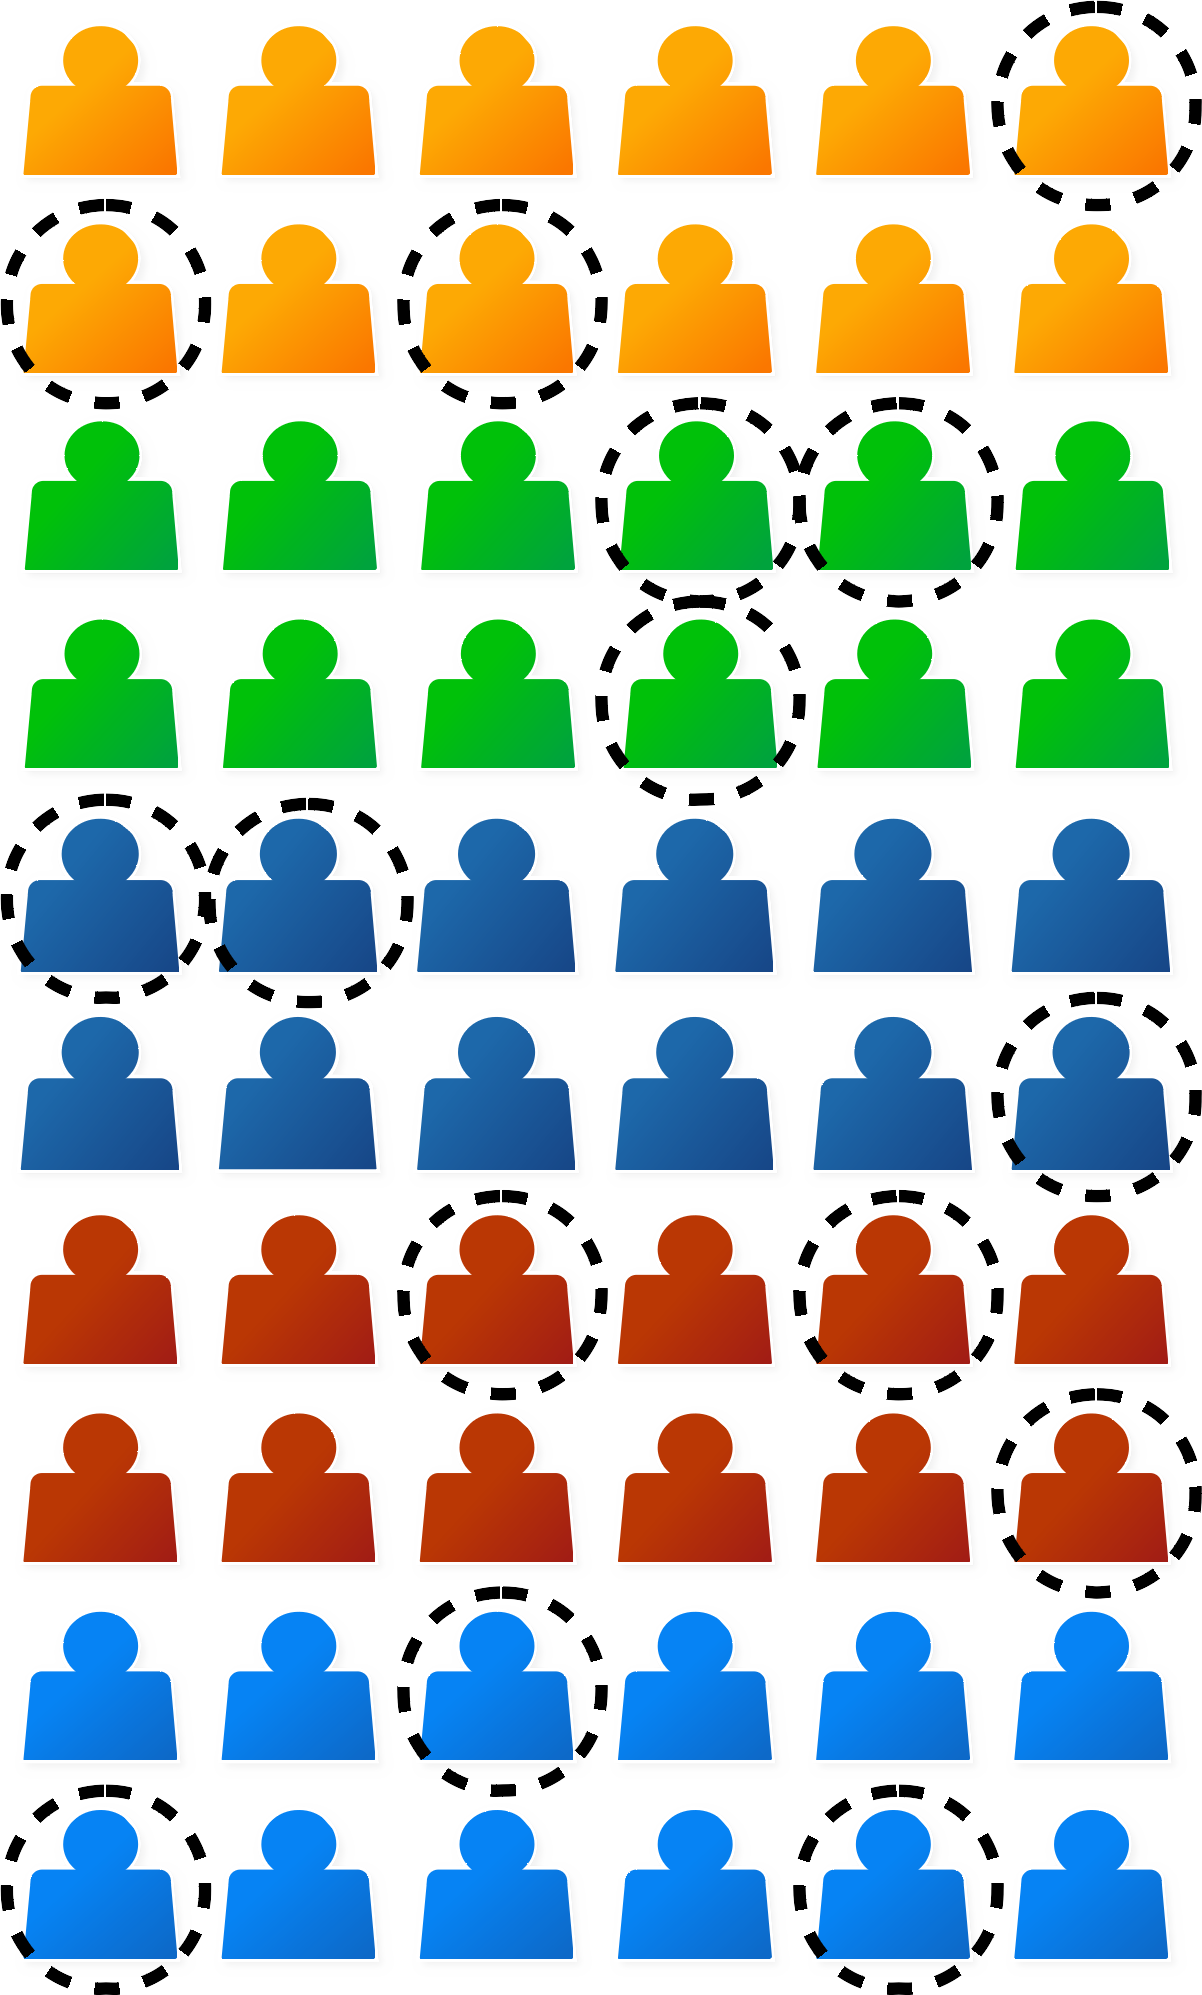
\includegraphics[width=\maxwidth{.35\linewidth}]{gfx/07-04}
	\caption{Stratified Sampling}
	\label{07:fig04}
\end{figure}

\textbf{Cluster Sampling} If the population is dispersed over a wide geographic region it may not be feasible to conduct a simple random sampling of the entire population. In such case, it may be reasonable to divide the population into ``clusters'' (typically along geographic boundaries), randomly select only a few clusters, and then measure all units within that cluster. For instance, to sample city governments in the state of New York, rather than travel all over the state to interview key city officials (as would be necessary with a simple random sample), the cities could be clustered by county and then all city officials in a randomly-selected group of counties would be interviewed. However, depending on between-cluster differences, the variability of sample results from a cluster sample will generally be higher than for a simple random sample so the results would be less generalizable to the population.

Figure \ref{07:fig05} illustrates cluster sampling. In this case, the population was divided into five clusters and then clusters three and four were randomly selected for the research project.

\begin{figure}[H]
	\centering
	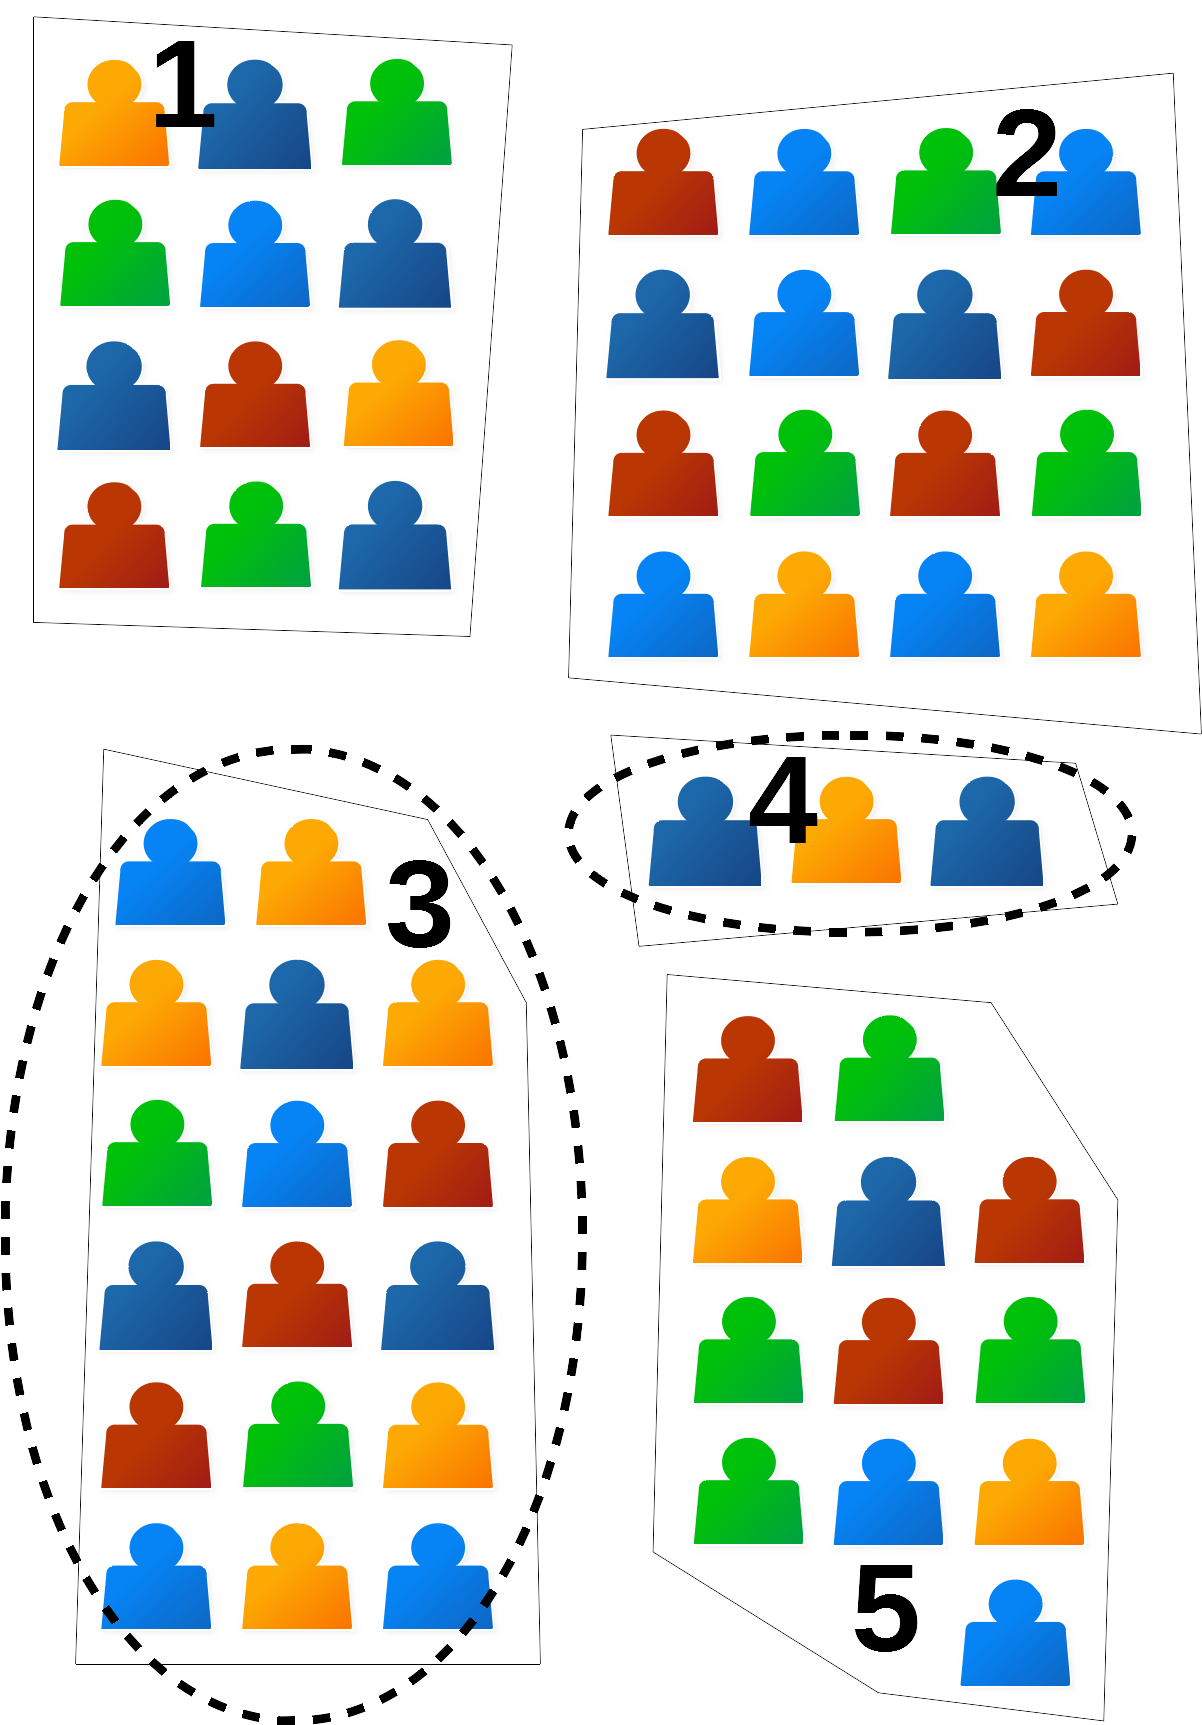
\includegraphics[width=\maxwidth{.35\linewidth}]{gfx/07-05}
	\caption{Cluster Sampling}
	\label{07:fig05}
\end{figure}

\textbf{Matched-pair Sampling} Sometimes, researchers may want to compare two subgroups within one population based on a specific criterion; for example, why are some firms consistently more profitable than others? To conduct such a study, the sampling frame of firms would be categorized into ``high profitable'' and ``low profitable'' firms based on gross margins, earnings per share, or some other measure of profitability. Then, a simple random sample of firms in one subgroup is selected. Each of those firms would be matched with one in the other subgroup based on its size, industry segment, or other criteria. Now, each of the firms can be studied in greater detail to look for reasons to explain their differences. Such matched-pairs sampling technique is often an ideal way of understanding bipolar differences between subgroups within a given population.

Figure \ref{07:fig06} illustrates matched pair sampling. In this case, one blue, green, and red element was selected at random and then matched with a similar element for comparison.

\begin{figure}[H]
	\centering
	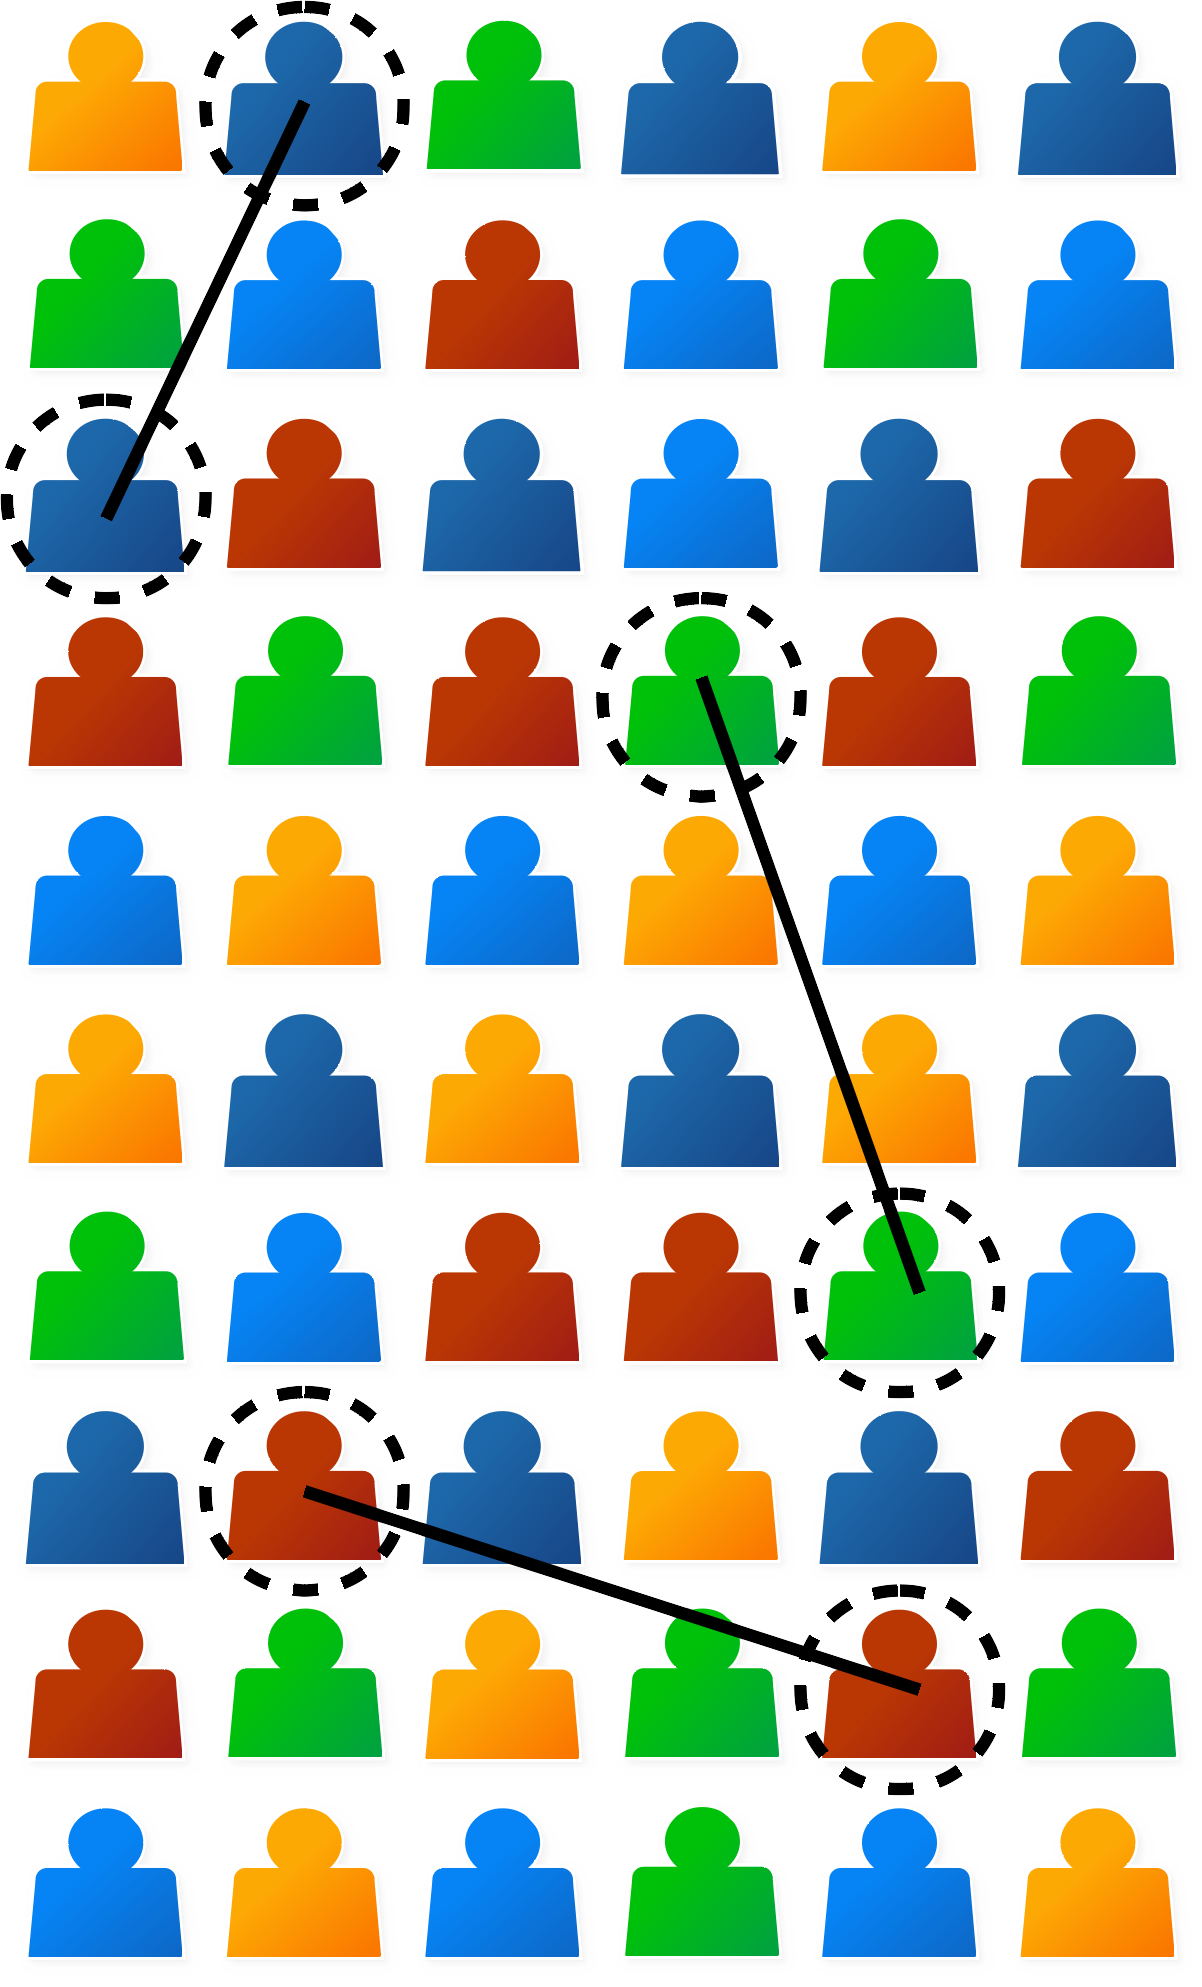
\includegraphics[width=\maxwidth{.35\linewidth}]{gfx/07-06}
	\caption{Matched Pair Sampling}
	\label{07:fig06}
\end{figure}

\textbf{Multi-stage Sampling} The sampling techniques described previously are all examples of single-stage sampling; however, they can be combined to conduct multi-stage sampling. For instance, a list of firms can be stratified based on size and then a systematic sampling can be conducted within each stratum. This would be a two-stage combination of stratified and systematic sampling. As a second example, a cluster of school districts in the state of Florida could be constructed and then a simple random sample of schools taken within each cluster, then a simple random sample of grade levels within each school, and, finally, a simple random sample of students taken from each grade level. This would constitute a four-stage sampling process consisting of cluster and simple random sampling.

\section{Sampling in Qualitative Research}

Qualitative researchers typically make sampling choices that enable them to deepen their understanding of the phenomenon being studied. Non-probability sampling is a sampling technique in which some units of the population have zero chance of selection or where the probability of selection cannot be accurately determined. Typically, units are selected based on certain non-random criteria, such as quota or convenience. Because selection is not random, the sampling error cannot be estimated in non-probability sampling, and it may be subject to sampling bias. Also, the samples will not exhibit a normal distribution so statistics like mean and standard deviation are of no value. As a result, information from a non-probability sample cannot be generalized back to the entire population. 

Non-probability samples are ideal during the design phase of a research project. For example, a survey can be administered to only a few people who seem to resemble the population being investigated in order to help work out problems with the survey. A non-probability sample is also useful for some exploratory research project where the goal is to determine if there is a need to conduct a more extensive project. Researchers also use non-probability sampling as the primary means of data collection in extensive qualitative research projects where the researcher's goal is in-depth, \gls{idiographic} understanding rather than more general, \gls{nomothetic} understanding. Thus, researchers who are interested in contributing to the theoretical understanding of some phenomenon might use non-probability samples. 

Types of non-probability sampling techniques include the following.

\textbf{Convenience Sampling} This is sometimes called ``accidental'' or ``opportunity'' sampling and is a technique in which a sample is drawn from that part of the population that is close to hand, readily available, or convenient. For instance, if a researcher stood outside a shopping center and surveyed shoppers as they walk in it would form a convenience sample. This is a non-probability sample because shoppers at other shopping centers are systematically excluded from the survey. The results of the survey may reflect the unique characteristics of this particular shopping center, such as the nature of its stores, the demographic profile of its patrons, or its location, but would not be representative of the opinions of the shopper population at large. Hence, the scientific generalizability of such observations will be very limited. Other examples of convenience sampling are sampling students registered in a certain class or sampling patients arriving at a certain medical clinic. This type of sampling is most useful for pilot testing, where the goal is instrument testing or measurement validation rather than obtaining generalizable inferences.

Figure \ref{07:fig07} illustrates convenience sampling where the researcher in the top left corner only samples the nearby elements and ignores the rest.

\begin{figure}[H]
	\centering
	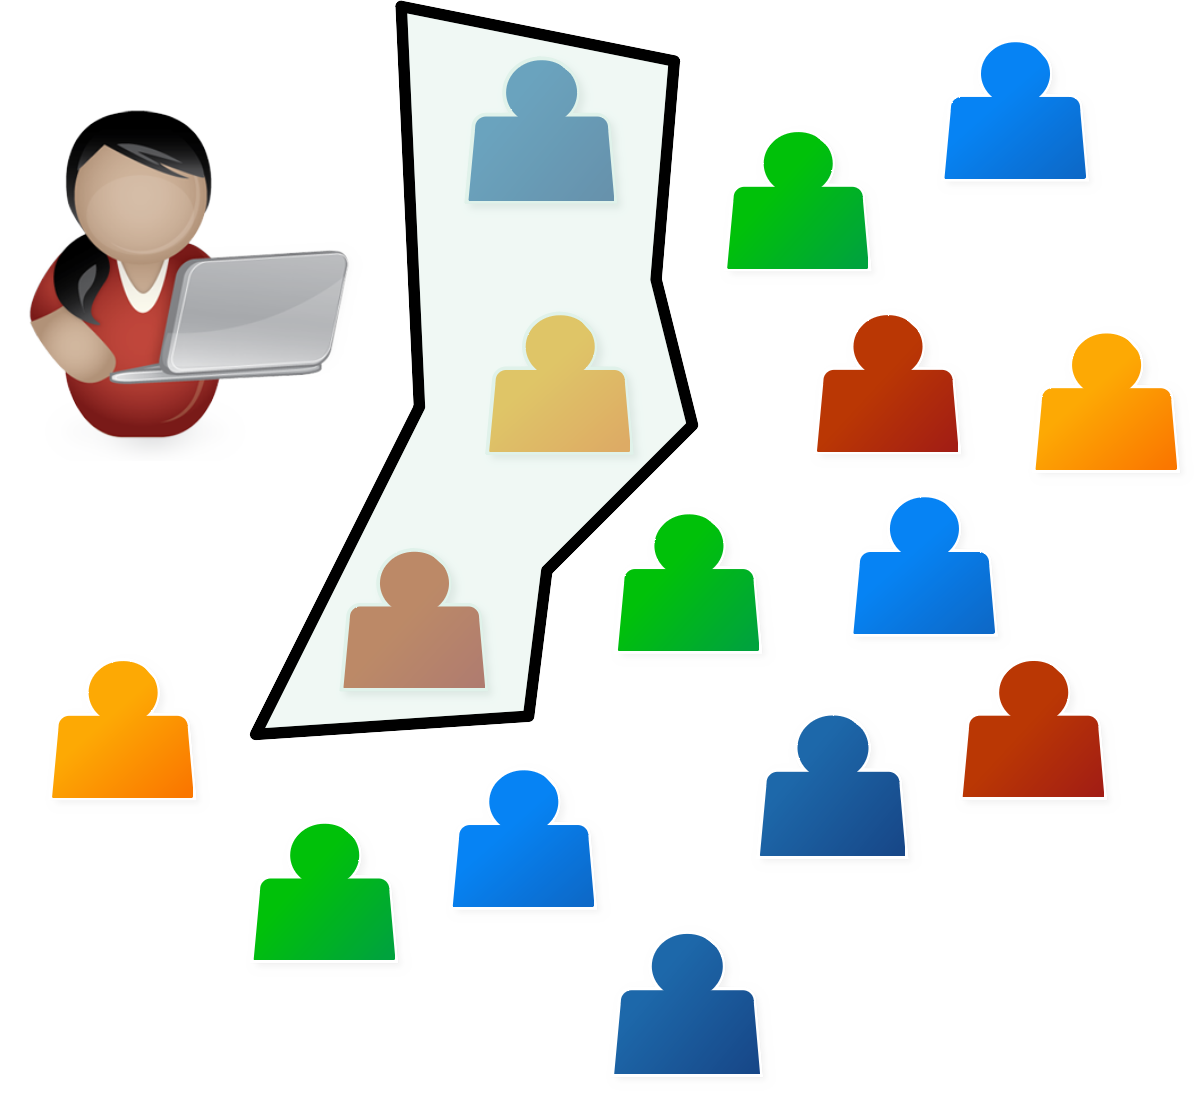
\includegraphics[width=\maxwidth{.35\linewidth}]{gfx/07-07}
	\caption{Convenience Sampling}
	\label{07:fig07}
\end{figure}

\textbf{Quota Sampling} In this technique, the population is segmented into mutually exclusive subgroups (just as in stratified sampling), and then a non-random set of observations is chosen from each subgroup to meet a predefined quota. In proportional quota sampling, the proportion of respondents in each subgroup should match that of the population. For instance, if the American population consists of 70\% Caucasians, 15\% Hispanic-Americans, and 13\% African-Americans, and researchers wished to understand their voting preferences in an sample of $ 100 $ people, they could stand outside a shopping center and ask people their voting preferences. But they would have to stop asking Hispanic people when they have $ 15 $ responses from that subgroup (or African-Americans when they have $ 13 $ responses) even as they continue sampling other ethnic groups. The goal is that the ethnic composition of the sample matches that of the general American population. Non-proportional quota sampling is less restrictive in that it does not have to achieve a proportional representation but does, perhaps, meet a minimum size in each subgroup. In this case, researchers may decide to have $ 50 $ respondents from each of the three ethnic subgroups (Caucasians, Hispanic-Americans, and African-Americans) and then stop when the quota for each subgroup is reached. Neither type of quota sampling will be representative of the American population, since depending on whether the study was conducted in a shopping center in New York or Kansas, the results may be entirely different. The non-proportional technique is even less representative of the population but may be useful in that it allows capturing the opinions of small and underrepresented groups through oversampling.

Figure \ref{07:fig08} illustrates quota sampling. In this case, a random sample is drawn from each of the subgroups but the larger subgroups have more samples than the smaller subgroups.

\begin{figure}[H]
	\centering
	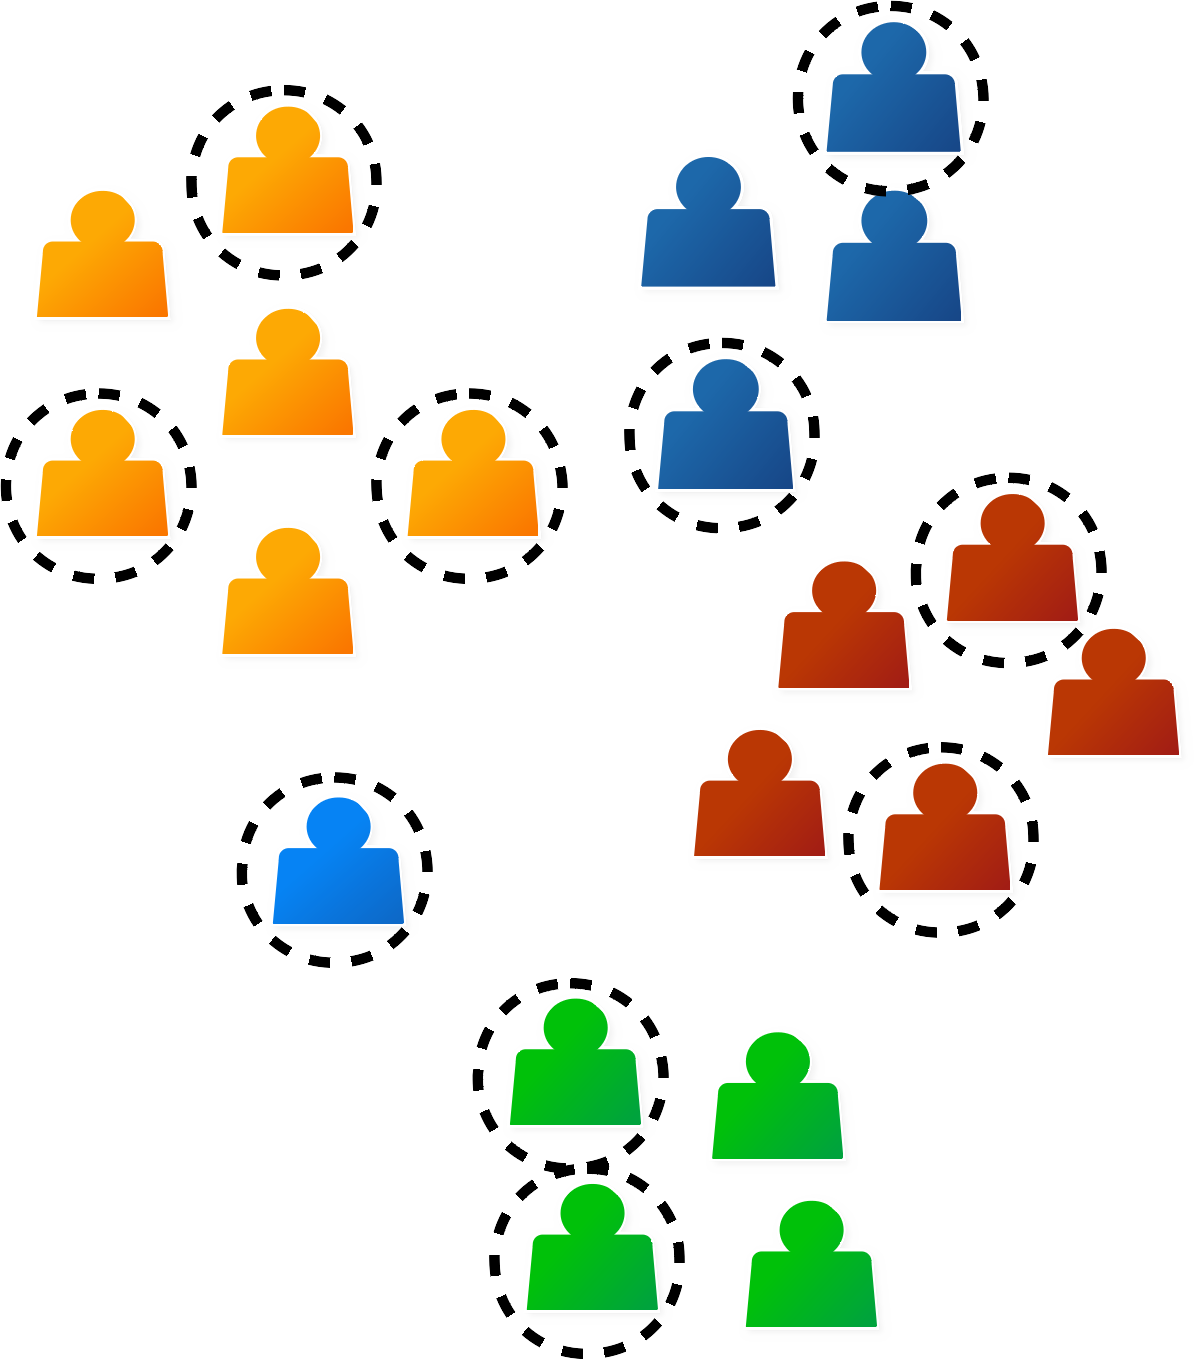
\includegraphics[width=\maxwidth{.35\linewidth}]{gfx/07-08}
	\caption{Quota Sampling}
	\label{07:fig08}
\end{figure}

\textbf{Snowball Sampling} In snowball sampling, a researcher starts by identifying a few respondents who match the criteria for inclusion in the study, and then asks those respondents to recommend others they know who would also meet the selection criteria. Snowball sampling is sometimes referred to as chain referral sampling since each respondent is also asked to provide the names of other potential respondents. After a few rounds, the researcher would have a large number of respondents, like a snowball getting larger as it rolls down a mountain. For example, if a researcher wishes to survey computer network administrators but only knows one or two then those people could recommend their peer network administrators and that group could recommend still others. Although this method hardly leads to representative samples, it may sometimes be the only way to reach hard-to-reach populations or when no sampling frame is available.

Figure \ref{07:fig09} illustrates snowball sampling. In this case, the researcher asked only one person, who recommended one other, who recommended two more, and so forth. In the end, the researcher sampled eight people but had only one to start the process.

\begin{figure}[H]
	\centering
	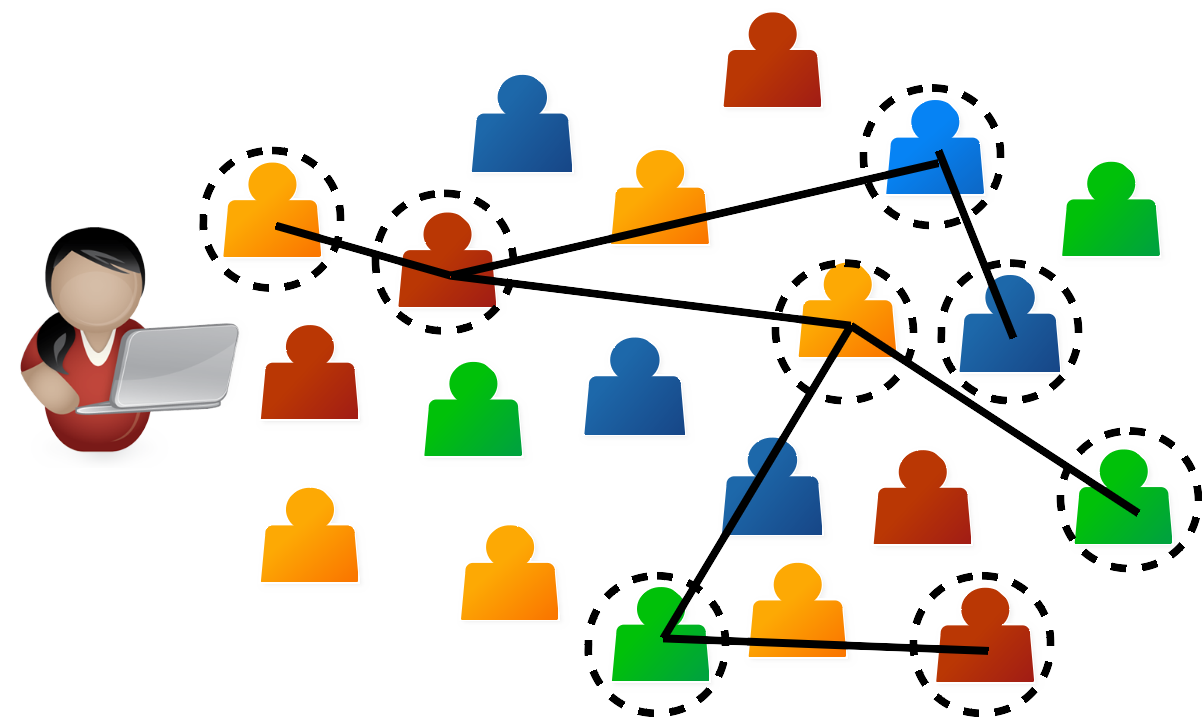
\includegraphics[width=\maxwidth{.35\linewidth}]{gfx/07-09}
	\caption{Snowball Sampling}
	\label{07:fig09}
\end{figure}

\textbf{Purposive Sampling} To draw a purposive sample, a researcher begins with specific perspectives to examine and then seeks research participants who exhibit the full range of perspectives. For example, a researcher studying students' satisfaction with their living quarters on campus would want to be sure to include students who stay in each of the different types or locations of on-campus housing. If only students from one of the ten dorms on campus are included then important details about the experiences of students who live in the other nine dorms would be missed. 

\textbf{Expert Sampling} This is a technique where respondents are chosen in a non-random manner based on their expertise on the phenomenon being studied. For instance, in order to understand the impacts of a new governmental policy such as the \textit{Sarbanes-Oxley Act}, a group of corporate accountants who are familiar with this act would be sampled. The advantage of this approach is that since experts tend to be more familiar with the subject matter than nonexperts, opinions from a sample of experts are more credible than a sample that includes both experts and non-experts, although the findings are still not generalizable to the overall population at large.


\section{Statistics of Sampling}

The preceding discussion introduced terms such as population, parameter, sample statistic, and sampling bias. This section defines these terms, and others, and illustrates how they are used and reported in a research project.

For this discussion, consider the data seen in Figure \ref{07:fig10}. This is a data set that represents the responses to a restaurant web survey such as is common in many fast food places. In this data, the attributes (columns) are a customer identification, the store number, the date and time a purchase was recorded, the purchase made (in coded form), and the answers to four questions, Q1-Q4. One column, illustrated in green, represents all responses to a single attribute, Q1 in this case. One observation (row) is highlighted in blue and represents all of the responses by a single customer.

\begin{figure}[H]
	\centering
%	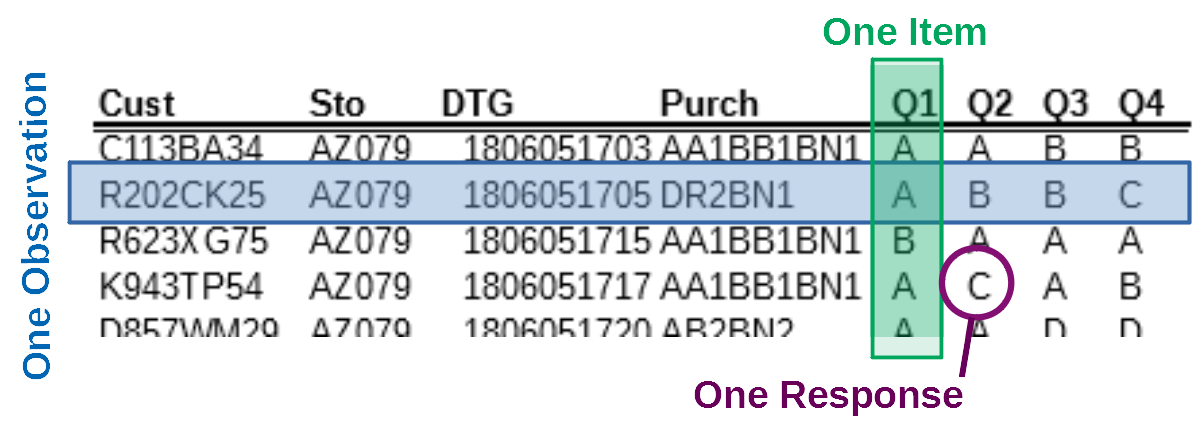
\includegraphics[width=\maxwidth{.95\linewidth}]{gfx/07-10}
	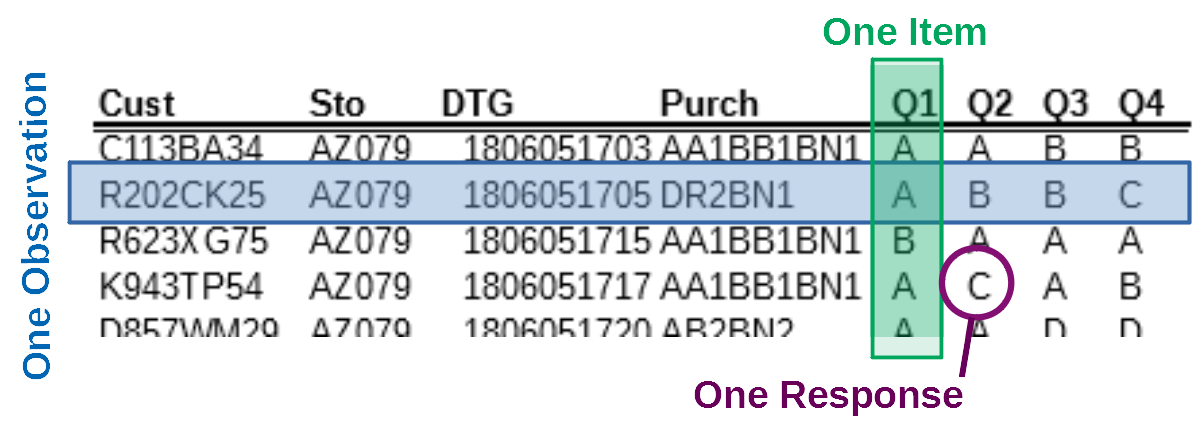
\includegraphics[]{gfx/07-10}
	\caption{Statistics Terms}
	\label{07:fig10}
\end{figure}

A specific observation of a phenomenon, such as a person's answer to a item Q2, is called a \textit{response}. In other words, a response is one point of measurement provided by a sampled unit (a customer). Researchers would expect each respondent to potentially provide different responses to the items in a survey. All responses for a single item, or a single column of data, can be analyzed in many different ways. If the item has categorical data, that is, data that are in categories, then the responses can be graphed into a frequency distribution based on their frequency of occurrences. For the survey results in \ref{07:fig10}, the responses to Q2 can only be A, B, C, or D since those were the only selections possible; and that makes Q2 categorical data. A frequency distribution for Q2 could look something like this

\begin{figure}[H]
	\centering
	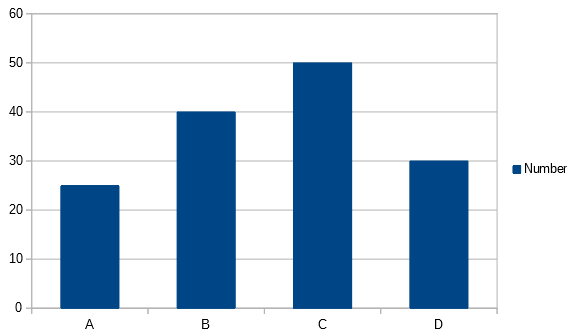
\includegraphics[width=\maxwidth{.95\linewidth}]{gfx/07-12}
	\caption{Frequency Chart}
	\label{07:fig12}
\end{figure}

Thus, the researcher could report that $ 40 $ people selected response B while $ 50 $ selected response C. If a sample has a large number of responses, the frequency distribution tends to resemble a normal distribution and that can then be used to estimate overall characteristics of the entire sample. Data that are continuous in nature, such as measurements, can have various characteristics calculated, like the sample mean or standard deviation. These sample estimates are called sample statistics (a ``statistic'' is a value that is estimated from observed data). 

Populations also have means and standard deviations that could be obtained if we could sample the entire population; however, since the entire population can usually not be sampled, population characteristics are always unknown and are called population parameters (not ``statistic'' because they are not statistically estimated from data). Sample statistics may differ from population parameters if the sample is not perfectly representative of the population. For example, the sample mean may be $ 45 $ while the population parameter is $ 48 $, and the difference between the two is called ``sampling error.'' Theoretically, if sample size could be gradually increased so the sample size approaches that of the population then the sampling error will decrease and a sample statistic will increasingly approximate the corresponding population parameter. In reality, though, it is usually not possible to have a sample size equal to the population.

If a sample is truly representative of the population, then the estimated sample statistics should be identical to corresponding population parameters and to estimate how closely those align a sampling distribution is used. 

\begin{figure}[H]
	\centering
%	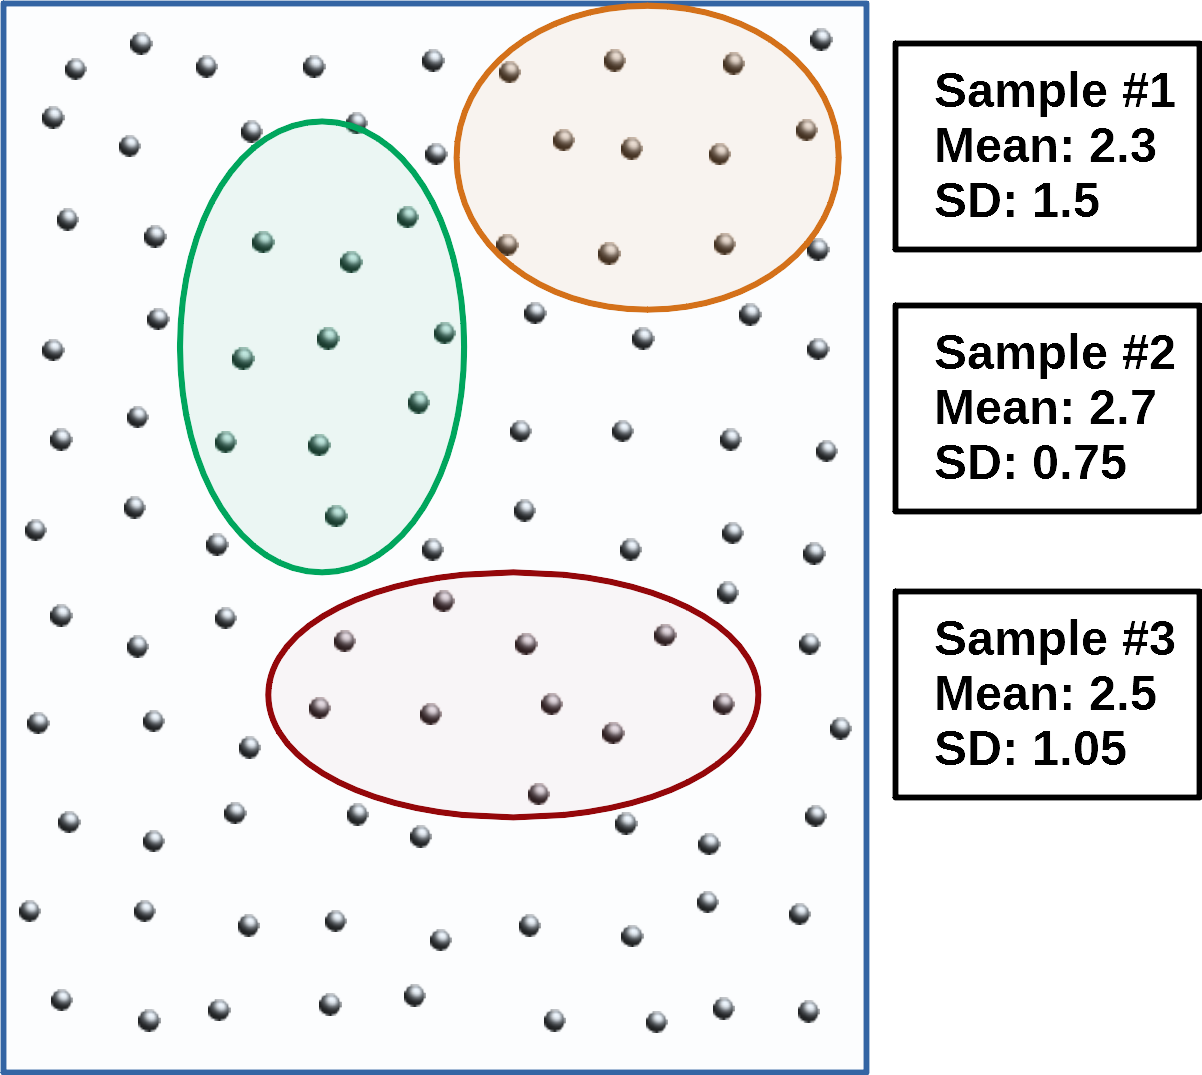
\includegraphics[width=\maxwidth{.95\linewidth}]{gfx/07-13}
	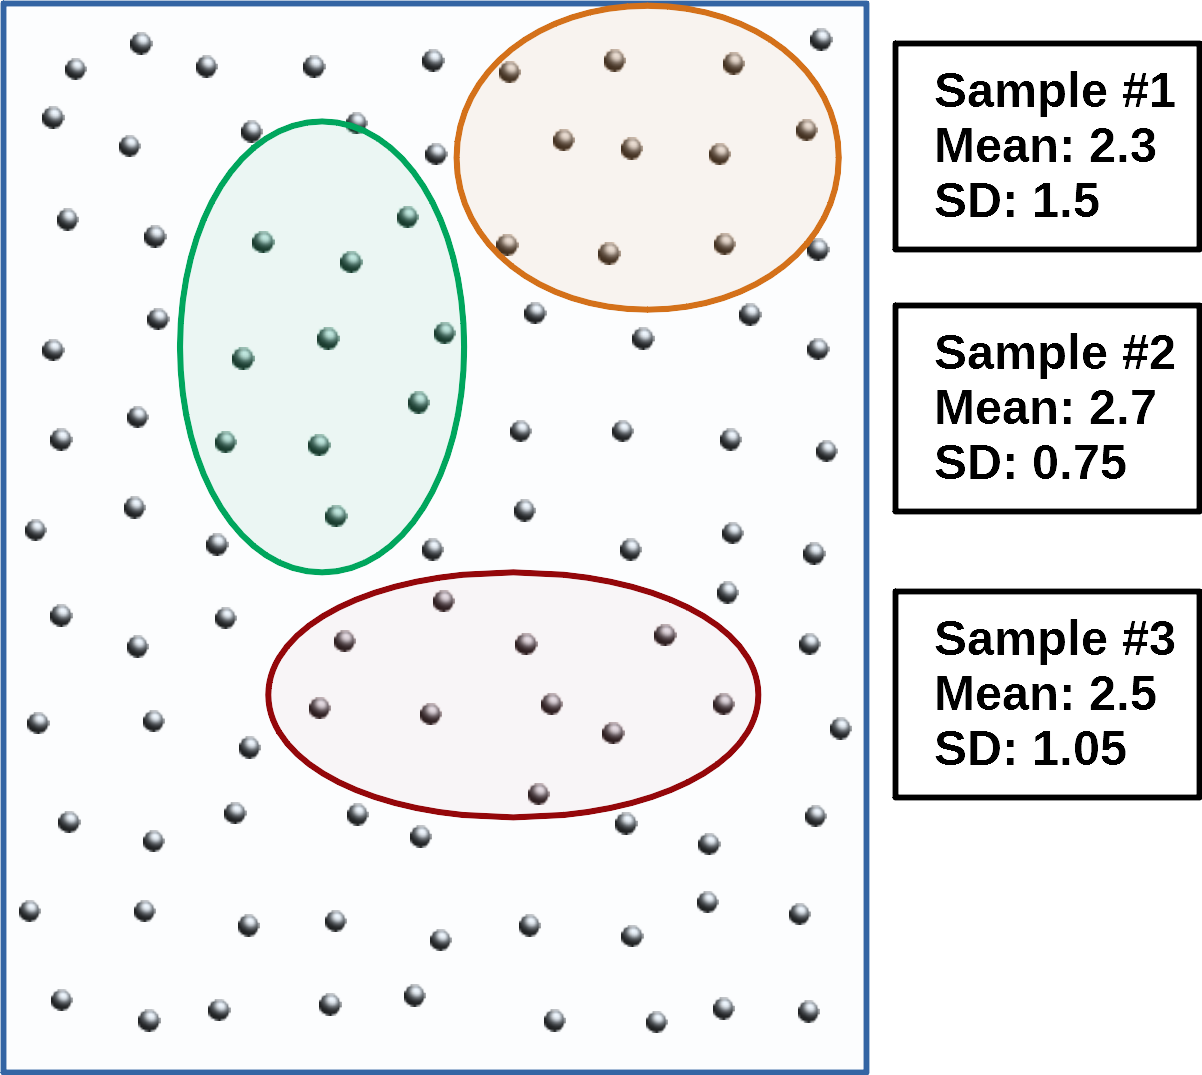
\includegraphics[]{gfx/07-13}
	\caption{Sample Statistics}
	\label{07:fig13}
\end{figure}

Figure \ref{07:fig13} illustrates the data from a research project. Imagine that three different random samples are drawn from the population and the mean and standard deviation are calculated for each sample. If each random sample was perfectly representative of the population, then the means and standard deviations from the three samples will be identical and equal to the population parameter. But this is extremely unlikely since each random sample will likely constitute a different subset of the population so their calculated statistics will be slightly different from each other. 

If the mean of the three sample means is calculated then it would be possible to also calculate the variability (or spread) of those means and that calculation is called the \textit{standard error of the mean}. The method to calculate that number is beyond the scope of this book, but the standard error of the mean for Figure \ref{07:fig13} is 0.115.\footnote{Students interested in how this number was derived can find help online. One source is an online calculator: \url{https://www.calculator.net/standard-deviation-calculator.html} and a good non-technical explanation can be found at \url{http://www.assess.com/standard-error-mean/}  } 

As the number of samples drawn from the population increases the variance between the means of those samples tends to decrease and they approach the mean of the entire population. Also, as the number of samples increases the standard error of the mean decreases and approaches zero. The mean value of a sample is presumed to be an estimate of the population parameter and the standard error of the mean makes it is possible to estimate \textit{confidence intervals} for how well the statistical mean predicts the population parameter. Since the standard error is similar to the standard deviation for a group of samples, it can be said that:

\begin{itemize}
	\item (Sample statistic + one standard error) represents a $ 68\% $ confidence interval for the population parameter.
	\item (Sample statistic + two standard errors) represents a $ 95\% $ confidence interval for the population parameter.
	\item (Sample statistic + three standard errors) represents a $ 99\% $ confidence interval for the population parameter.
\end{itemize}

In Figure \ref{07:fig13}, the mean of the three samples is $ 2.5 $ and the standard error is $ 0.115 $. Therefore, any sample mean in the range of $ 2.385-2.615 $ has a $ 68\% $ chance of predicting the population mean, any sample mean in the range of $ 2.27-2.73 $ has a $ 95\% $ chance of predicting the population mean, and any sample mean in the range of $ 2.155-2.845 $ has a $ 99\% $ chance of predicting the population mean. Since sample one falls in the $ 95\% $ confidence band a researcher could predict that $ 2.3 $ (the mean of that sample) predicts the mean of the entire population with a $ 95\% $ confidence level.

\section{Sample Size}

When working with sampling one of the first questions researchers face is the sample size. In other words, how many observations are needed to have a useful sample. In general, the larger the sample the more accurately it will represent the population and the more robust the statistical analysis is possible. Unfortunately, the answer to the question about sample size is a bit nebulous. One rule of thumb that many researchers mention is a minimum of $ 30 $, but that is a gross oversimplification and does not work well except in classroom-size projects. When determining an appropriate sample size, a number that is too small may exclude parts of the population while a number that is too large may become unwieldy for the researcher. 

Determining an appropriate sample size is a mix of both mathematics and experience. There are formulas that will help researchers determine a good sample size, but those must be tempered with experience and an understanding of the population being studied. For example, if a formula indicated that a sample size of $ 250 $ is appropriate for a population of $ 500 $ people but the researcher happens to know that the population is very diverse with many racial or ethnic groups then the sample may need to be increased to ensure that all groups are fairly represented.

To make researcher's jobs easier, numerous sample size tables have been published and it is easy to refer to these tables to determine a good sample size. Figure \ref{07:fig14} shows a very simple such table\cite{israel1992determining}.

\begin{figure}[H]
	\centering
	%	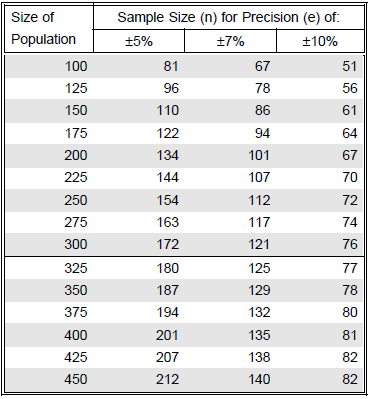
\includegraphics[width=\maxwidth{.35\linewidth}]{gfx/07-14}
	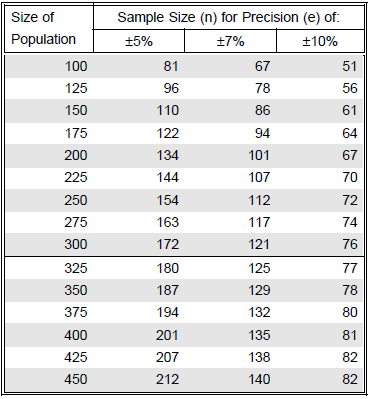
\includegraphics[width=4in]{gfx/07-14}
	\caption{Sample Size For Confidence Level of 95\%}
	\label{07:fig14}
\end{figure}

In the table in Figure \ref{07:fig14}, the confidence level is $ 95\% $ for all values. This is a typical confidence level and is commonly used in the statistical analysis of a data set. Very frequently, that confidence level is expressed as a ``p'' value of $ 0.05 $. Precision, in this case, is defined as how close the estimates from different samples are to each other. The smaller the precision then the closer the values in each sample will be to each other and, presumably, to the population parameter. As an example from the table in Figure \ref{07:fig14}, if a researcher were conducting a survey for a population of $ 400 $ and desired $ 5\% $ precision then $ 201 $ samples would need to be taken.

\section{A Word of Caution}

It is easy to overlook the need to ask important questions about where research participants come from and how they are identified for inclusion in a research project, in other words, how the sample was determined. It is easy to focus only on the interesting stuff in the findings, but understanding the procedures used for selecting study participants is critical.

Students who have ever taken an introductory psychology or sociology class at a large university are very frequently drafted into research projects since that is an easy group for graduate students to access. But that access comes at a cost: sample representativeness. One study of top academic journals in psychology found that over two-thirds ($ 68\% $) of participants in studies published by those journals were based on samples drawn in the United States\cite{arnett2008neglected} Further, the study found that two-thirds of the work that derived from United States samples published in the Journal of Personality and Social Psychology was based on samples made up entirely of American undergraduates taking psychology courses.

These findings raise an interesting the question: What do we actually learn from social scientific studies and about whom do we learn it? That is exactly the concern raised by Joseph Henrich and colleagues\cite{henrich2010most} who point out that behavioral scientists very commonly make sweeping claims about human nature based on samples drawn only from WEIRD (Western, Educated, Industrialized, Rich, and Democratic) societies, and often based on even narrower samples, as is the case with many studies relying on samples drawn from college classrooms. As it turns out, many robust findings about the nature of human behavior when it comes to fairness, cooperation, visual perception, trust, and other behaviors are based on studies that excluded participants from outside the United States and sometimes excluded anyone outside the college classroom. This certainly raises questions about what we really know about human behavior as opposed to that of United States undergraduate behavior. Of course not all research findings are based on samples of WEIRD folks like college students. But even then it is important to pay attention to the samples on which studies are based and the claims that are being made about to whom those studies apply.

In the preceding discussion, the concern is with researchers making claims about populations other than those from which their samples were drawn. A related, but slightly different, potential concern is sampling bias. Bias in sampling occurs when the elements selected for inclusion in a study do not represent the larger population from which they were drawn. For example, an on-line poll conducted by a newspaper asking for an opinion about some local issue will certainly not represent the public since those without access to computers or the Internet, those who do not read that paper's website, and those who do not have the time or interest will not answer the question.

Another thing to keep in mind is that just because a sample may be representative in all respects that a researcher thinks are relevant, there may be aspects that are relevant that did not occur to the researcher. For example, peoples' phones would seem to have little to do with their voting preferences but had pollsters making predictions about the results of the $ 2008 $ presidential election not been careful to include both cell phone and land line households in their surveys, it is possible that their predictions would have underestimated Barack Obama's lead over John McCain because Obama was much more popular among cell-only users than McCain\cite{keeter2008calling}.

When evaluating a research report, remember that sample quality is determined only by the sample actually obtained, not by the sampling method itself. A researcher may set out to administer a survey to a representative sample by correctly employing a random selection technique, but if only a handful of the people sampled actually respond to the survey, the researcher will have to be very careful about the claims made. Another thing to keep in mind is that researchers discuss the implications of their findings as though they apply to some group other than the population actually sampled. This tendency is usually innocent since it is human nature to inflate the applicability of the findings; but consumers of those findings must be attentive to this sort of (hopefully unintentional) bait and switch. 

At their core, questions about sample quality should address who has been sampled, how they were sampled, and for what purpose they were sampled. Being able to answer those questions will improve understanding of the research results.

\section{Summary}

\begin{itemize}
	\setlength{\itemsep}{0pt}
	\setlength{\parskip}{0pt}
	\setlength{\parsep}{0pt}
	
	\item To be provided.
	\item To be provided.
	
\end{itemize}

%%*****************************************
\chapter{Survey Research}\label{08:surveys}
%*****************************************

\begin{wrapfigure}{R}{0.4\textwidth}
	\label{08:fig01} 
	\centering
	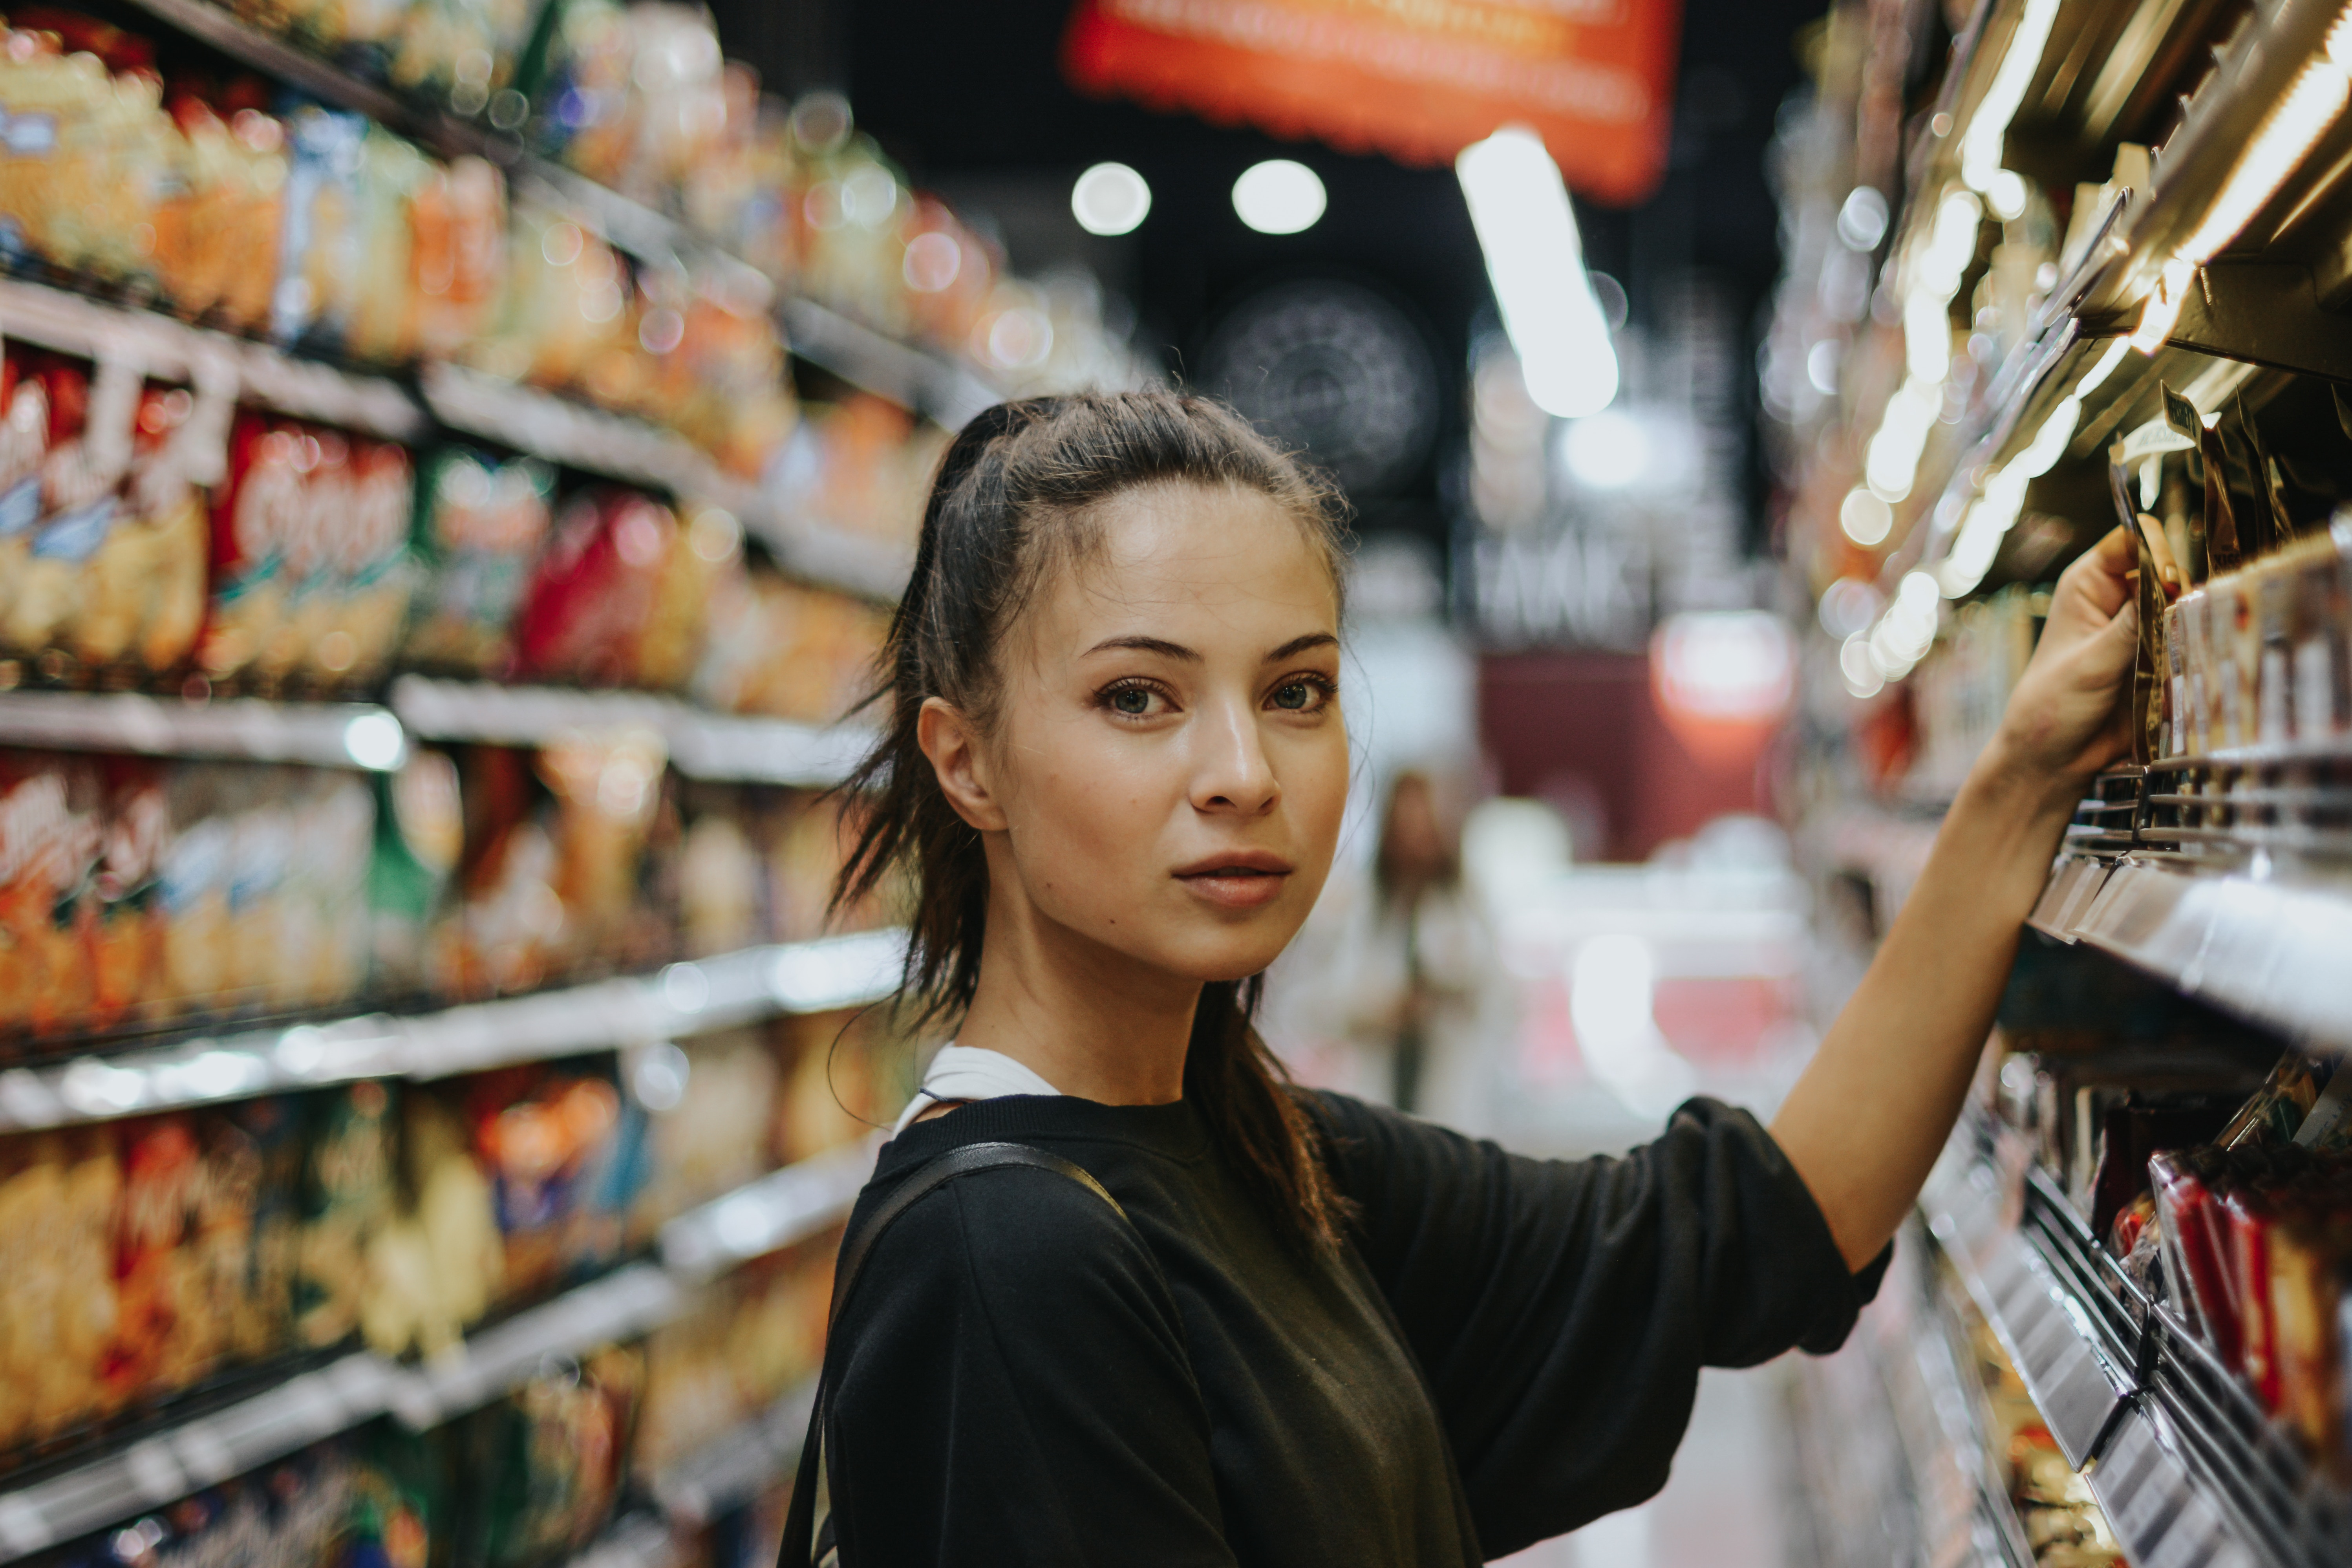
\includegraphics[width=0.4\textwidth]{gfx/08-01} 
\end{wrapfigure}

How do retailers know what sorts of products their customers are likely to purchase? They use surveys to ask questions. Unfortunately, creating an unbiased survey that asks the right questions is a much more complex task than it may seem. This chapter introduces the art and science of survey design, from types of surveys, writing questions, and analyzing the results.
\blfootnote{Photo by Joshua Rawson-Harris on Unsplash}

\begin{center}
	\begin{objbox}{Objectives}
		\begin{itemize}
			\setlength{\itemsep}{0pt}
			\setlength{\parskip}{0pt}
			\setlength{\parsep}{0pt}
			
			\item Differentiate between cross-sectional and longitudinal surveys
			\item Compare and contrast the four types of longitudinal surveys: trend, panel, cohort, and retrospective
			\item Describe the characteristics of effective questions
			\item Define the various question response options
			\item Describe tips for creating good questionnaires
			\item Discuss how survey data are analyzed
			\item Discuss bias in survey research
		\end{itemize}
	\end{objbox}
\end{center}

\section{Introduction}

\Gls{survey} research is a method involving the use of standardized questionnaires or interviews to collect data about people and their preferences, thoughts, and behaviors in a systematic manner. Although census surveys were conducted as early as Ancient Egypt, using a survey as a formal research method was pioneered in the $ 1930-40 $s by sociologist Paul Lazarsfeld to examine the effects of the radio on political opinion formation of the United States. This method has since become a very popular method for quantitative research in business and social sciences. Because most students have completed many surveys, they often underestimate the skill and effort needed to create a valid survey. The process is time-consuming and tedious and requires many revisions.

The survey method is best suited for studies that have individual people as the unit of analysis. Although other units of analysis, such as groups, organizations or dyads (pairs of organizations, such as buyers and sellers), are also studied using surveys, such studies often use a specific person from each unit as a ``key informant'' or a ``proxy'' for that unit, and such surveys may be subject to respondent \gls{bias} if the informant chosen does not have adequate knowledge or has a biased opinion about the phenomenon of interest. For instance, Chief Executive Officers may not adequately know employee's perceptions or teamwork in their own companies, and may therefore be the wrong informant for studies of team dynamics or employee self-esteem.

Survey research has several inherent strengths compared to other research methods. 

\begin{enumerate}
	\item Surveys are an excellent vehicle for measuring a wide variety of unobservable data, such as people's preferences (\eg, political orientation), traits (\eg, self-esteem), attitudes (\eg, toward immigrants), beliefs (\eg, about a new law), behaviors (\eg, smoking or drinking behavior), or factual information (\eg, income). 

	\item Survey research is also ideally suited for remotely collecting data about a population that is too large to observe directly. A large area, such as an entire country, can be covered using mail-in, electronic mail, internet, or telephone surveys using meticulous sampling to ensure that the population is adequately represented in a small sample. 

	\item Due to their unobtrusive nature and the ability to respond at one's convenience, questionnaire surveys are preferred by some respondents.

	\item Surveys are more easily generalized than other research techniques since data can be collected from very large samples at a relatively low cost.

	\item Because surveys are standardized in that the same questions, phrased in exactly the same way, are posed to all participants they tend to have higher \gls{reliability} than other methods of gathering data.

	\item Interviews may be the only way of reaching certain population groups such as the homeless or illegal immigrants for which there is no \gls{sampleframe} available. 

	\item Large sample surveys may allow detection of small effects even while analyzing multiple variables, and depending on the survey design, may also allow comparative analysis of population subgroups (i.e., within-group and between-group analysis). 

	\item Survey research is more economical in terms of researcher time, effort and cost than most other methods such as experimental research and case research.
\end{enumerate}

At the same time, survey research also has some disadvantages. 

\begin{enumerate}
	\item It is subject to a large number of \glspl{bias} such as non-response bias, sampling bias, social desirability bias, and recall bias (all of these are discussed later in this chapter).
	
	\item While surveys are flexible in the sense that any number of questions on any number of topics may be asked, the researcher is also stuck with that instrument even if it is later shown to contain confusing items. 
	
	\item Survey questions must be written such that a broad range of people will understand each of them. Because of this, survey results may suffer from \gls{validity} concerns not found in methods that are more flexible. 
\end{enumerate}

\section{Types of Surveys}

There is much variety when it comes to surveys. This variety comes both in terms of time, \ie\: when or how frequently a survey is administered, and administration, \ie\: how a survey is delivered to respondents. This section develops both types of concepts.

\subsection{Time}

In terms of time, there are two main types of surveys: \gls{crosssectional} and \gls{longitudinal}.

\subsubsection{Cross-Sectional}

Cross-sectional surveys are those that are administered at just one point in time. These surveys offer researchers a snapshot in time and provides an idea about how things are at the particular point in time. These surveys are call ``cross-sectional'' since they will take a snapshot across multiple analytical units. For example, a survey may be administered to staff members in the human resources department of five different companies or customers of several different movie theaters on the same evening. 

An example of a cross-sectional survey is a study of e-cigarette use among adolescents conducted by Dutra and Glantz\cite{dutra2014electronic}. They used a cross-sectional survey of more than $ 40,000 $ students from more than $ 200 $ middle and high schools across the United States. They determined that the use of e-cigarettes was ``...associated with higher odds of ever or current cigarette smoking...''

Another example of a cross-sectional survey, J\o{}rgensen, et. al.\cite{jorgensen2016does}, investigated if workplace health promotions depend on the work environment. They surveyed $ 10,605 $ Danish workers and determined that lower participation in health promotions is dependent on when they are offered (during or afterwork), the social support at work for the programs, and whether their work has high physical demands.

One problem with cross-sectional surveys is that the events, opinions, behaviors, and other phenomena that such surveys are designed to assess are generally not stagnant. Thus, generalizing from a cross-sectional survey about the way things are can be tricky. Perhaps something can be concluded about the way things \textit{were} in the moment that the survey was administered, but it is difficult to know whether things remained that way afterwards. For example, imagine how Americans might have responded to a survey about terrorism on September $ 10 $, $ 2001 $, compared to September $ 12 $, $ 2001 $. The point is not that cross-sectional surveys are useless, but researchers must remember that these surveys are a snapshot in time.

\subsubsection{Longitudinal}

Longitudinal surveys are those that include observations made over some extended period of time. There are four types of longitudinal surveys: trend, panel, cohort, and retrospective.

\paragraph{Trend Survey}

The first type of longitudinal survey is a trend survey. This type of study takes place over a long period of time, often years, and involves multiple surveys of many different people. As one example of a trend survey, Dobrow, Ganzach, and Liu\cite{dobrow2015time} studied job satisfaction in light of employee's age and tenure. They surveyed $ 21,670 $ people in $ 34 $ ``waves'' of data collection spanning $ 40 $ years. They found that as tenure in an organization increased people tend to be less satisfied with their jobs, however, as people age and move from job to job their satisfaction increased.

\paragraph{Panel Surveys}

Unlike a trend survey, a panel survey uses the same people each time it is administered. As you might imagine, panel studies can be difficult and costly. Imagine trying to administer a survey to the same $ 100 $ people every year for five years in a row. Keeping track of where people live, when they move, and when they die takes resources that researchers often do not have. Panel surveys, however, can be quite powerful. 

The \gls{yds}\cite{uminn2018youth}, administered by the University of Minnesota, is an excellent example of a panel study. Since $ 1988 $, \gls{yds} researchers have administered an annual survey to the same $ 1,000 $ people. Study participants were in ninth grade when it began and they are now in their thirties. Several hundred papers, articles, and books have been written using data from the \gls{yds}. One of the major lessons learned from this panel study is that work has a largely positive impact on young people. Contrary to popular belief about the impact of work on adolescents' performance in school and transition to adulthood, work increases confidence, enhances academic success, and prepares students for success in their future careers. This panel study provided important information about the affect of work on young people.

As an example of a panel survey for business, Huhtala, Kaptein, and Feldt conducted a two-year study concerning how the ethical culture of organizations influence the well-being of managers\cite{huhtala2016perceived}. They found that managers in low or decreasing ethical cultures experienced changes in their well-being over the two years of the study.

\paragraph{Cohort Surveys}

In a cohort survey, a researcher identifies some category of people that are of interest and then regularly surveys the people who fall into that category. The same people do not necessarily participate from year to year, but all participants must meet whatever categorical criteria fulfill the researcher's primary interest. Common cohorts that may be of interest to researchers include people of particular generations or those who were born around the same time period, graduating classes, people who began work in a given industry at the same time, or perhaps people who have some specific life experience in common. An example of this sort of research can be seen in Christine Percheski's work on cohort differences in women's employment\cite{percheski2008opting}. Percheski compared women's employment rates across seven different generational cohorts, from Progressives born between $ 1906 $ and $ 1915 $ to Generation Xers born between $ 1966 $ and $ 1975 $. She found, among other patterns, that professional women's labor force participation had increased across all cohorts. She also found that professional women with young children from Generation X had higher labor force participation rates than similar women from previous generations, concluding that mothers do not appear to be opting out of the workforce as some journalists have speculated.

In another cohort study, Wright and Hinson surveyed public relations practitioners over a ten-year period from $ 2005 $ until $ 2015 $\cite{wright2015examining}. While some of the same practitioners would have participated over that entire span, it is reasonable to assume that at least a few of the respondents changed during that period, but they were all public relations experts in a company. They found that both \textit{Facebook} and \textit{Twitter} were the dominant means of public relations communication while \textit{LinkedIn} and \textit{YouTube} were not as popular. The survey respondents, though, agreed that social media were changing the way public relations is practiced. It would be interesting to see how the perceptions of public relations experts have changed since $ 2016 $ given the heavy reliance on \textit{Twitter} in the United States by President Donald Trump.

All three types of longitudinal surveys share the strength that they permit a researcher to make observations over time. This means that if whatever behavior or other phenomenon the researcher is interested in changes, either because of some world event or because people age, the researcher will be able to capture those changes. 

\paragraph{Retrospective Surveys}

Retrospective surveys are similar to other longitudinal studies in that they concern changes over time, but like a cross-sectional study, they are administered only once. In a retrospective survey, participants are asked to report events from the past. By having respondents report past behaviors, beliefs, or experiences, researchers are able to gather longitudinal-like data without actually incurring the time or expense of a longitudinal survey. Of course, this benefit must be weighed against the possibility that people's recollections of their pasts may be faulty. Imagine, for example, that people are asked in a survey to respond to questions about where, how, and with whom they spent last Valentine's Day. Since Valentine's Day cannot be more than $ 12 $ months ago, chances are good that they may be able to respond accurately. But if the question is to compare last Valentine's Day with the six previous Valentine's Days the result would be much different.

Table \ref{tab08.01} summarizes each of the four types of longitudinal survey.

\begin{table}[H]
	\centering
	\definecolor{ltgray}{gray}{0.95} % this is a light gray
	\rowcolors{1}{}{ltgray} % zebra striping background
	\begin{tabularx}{0.95\linewidth}{p{0.15\linewidth}p{0.75\linewidth}}
		\toprule
		\textbf{Type} & \textbf{Description} \\
		\midrule
		Trend & Researcher examines changes in trends over time; the same people do not necessarily participate in the survey more than once. \\
		Panel & Researcher surveys the exact same sample several times over a period of time. \\
		Cohort & Researcher identifies some category of people that are of interest and then regularly surveys people who fall into that category.\\
		Retrospective & Surveys are conducted only one time but the respondents are asked to report of things that happened in the past.\\		
		\bottomrule
	\end{tabularx}
	\caption{Compare the Four Types of Longitudinal Survey}
	\label{tab08.01}
\end{table}


\subsection{Administration}

Surveys vary not just in terms of when they are administered but also in terms of how they are administered. One common way to administer surveys is in the form of a self-administered \gls{questionnaire}. This means that research participants are given a set of questions, in writing, to which they are asked to respond. Self-administered questionnaires can be delivered in printed format, in a group setting, or online.

\paragraph{Printed Survey}

Printed self-administered questionnaires may be delivered to participants in person; for example, people who are gathered in one place, like students in class, members of a church, or inmates. Researchers may also hand-deliver questionnaires by going door-to-door and either asking people to fill them out right away or making arrangements for the researcher to return to pick up completed surveys. Though the advent of online survey tools has made the door-to-door delivery of surveys nearly extinct, an occasional survey researcher may still use this method, especially around election time.

If a researcher is not able to visit each member of the sample to personally deliver a survey, sending it through physical mail may be another consideration. While this mode of delivery may not be ideal (imagine how much less likely someone would be to return a survey where the researcher was not standing on the doorstep waiting), sometimes it is the only available or the most practical option.

Often survey researchers who deliver their surveys via physical mail may provide some advance notice to respondents about the survey to get people thinking about and preparing to complete it. They may also follow up a few weeks after their survey has been sent out. This can be done not only to remind those who have not yet completed the survey to please do so but also to thank those who have already returned the survey. Most survey researchers agree that this sort of follow-up is essential for improving mailed surveys' return rates\cite{babbie2010unobtrusive}.

\paragraph{Group Survey}

A second type of survey administration is a group-administered questionnaire. A sample of respondents is brought together at a common place and time and each respondent is asked to complete the survey questionnaire while in that room. Respondents typically sit at desks or in some sort of study carrel and enter their responses independently without interacting with each other. This format is convenient for the researcher and high response rate is assured. Also, if respondents do not understand any specific question, they can ask for clarification. These types of surveys are most useful in an organization where it is relatively easy to assemble a group of employees in a conference room or lunchroom, especially if the survey is approved by corporate executives.

\paragraph{Online Survey}

One final approach to delivering surveys is online. This delivery mechanism is becoming increasingly common, no doubt because it is easy to use, relatively cheap, and may be quicker than knocking on doors or waiting for mailed surveys to be returned. To deliver a survey online, researchers may subscribe to a service that offers online delivery or use some delivery mechanism that is available for free, like \textit{SurveyMonkey}. One advantage to using a service like \textit{SurveyMonkey}, aside from the advantages of online delivery, is that results can be provided in formats that are readable by data analysis programs such as \textit{R} and \textit{Excel}. This saves researchers the step of having to manually enter data into an analysis program, as is necessary for hard copy surveys.

There are several weaknesses for online surveys. If the survey website is not password-protected or designed to prevent multiple submissions, the responses can be easily compromised. Furthermore, sampling bias may be a significant issue since the survey cannot reach people who do not have computer or Internet access, such as many of the poor, senior, and minority groups; moreover, the respondent sample will be skewed toward a younger demographic who are online much of the time and have the time and ability to complete such surveys. Finally, computing the response rate may be problematic if the survey link is posted in \textit{Facebook}, \textit{Twitter}, or other social media sites instead of being e-mailed directly to targeted respondents. 

Many of the suggestions provided for improving the response rate on a printed questionnaire apply to online questionnaires as well. One difference, of course, is that the sort of incentive that can be provided in an online format differ from those that can be given in person or sent through the mail. Many online surveys only come with the incentive of knowing that the respondent is helping other people. It is possible, though, to provide some sort of coupon to an online store like \textit{Amazon}. Commonly, online surveys provide some sort of food, like a ``free large drink,'' from the restaurant that is administering the survey. Finally, it is possible to have respondents provide some sort of contact information, like an email address, and then have a drawing for a free \textit{Fire} tablet or some other prize. Using these sorts of rewards raises questions about the validity of the results. If people are only participating in a survey to have a chance at a prize then are they going to simply pattern-respond (choose all ``A'' answers, for example) or will they take the time to thoughtfully respond?

\paragraph{Other Types}

Sometimes surveys are administered by researchers posing questions directly to respondents rather than have them read the questions on their own. These types of surveys are a form of interview, which is discussed in Chapter \ref{ch10:interviews}. It is enough at this point to mention that interview methodology differs significantly from survey research in that data are collected via a personal interaction. 

\section{Designing Effective Questionnaires}

Invented by Sir Francis Galton, a \gls{questionnaire} is a research instrument consisting of a set of items intended to capture responses from respondents in a standardized format. Items may be either structured or unstructured. Structured items ask respondents to select an answer from a set of choices. The responses are then aggregated into a composite scale or index for statistical analysis. On the other hand, unstructured questions ask respondents to provide a response in their own words using a free-flow type of entry. Questions should be designed such that respondents are able to read, understand, and respond to them in a meaningful way so surveys would not be appropriate for certain demographic groups such as children or the illiterate. 

\subsection{Effective Questions}

The first thing needed to write effective survey questions is identifying what, exactly, is being sought. Though it seems obvious, missing important questions when designing a survey is far too common. Suppose researchers want to understand how students make a successful transition from high school to college and what factors contribute to that success. To understand those factors, the researchers will need to include questions about all of the possible factors that could contribute to success. They would consult the literature on the topic, but should also take the time for brainstorming and talking with other researchers (and even high school students) about what may be important in the transition to college. It may not be possible to include every single factor on a survey since that may make the survey pages long, but some thought would generate a list of the most important factors.

While it is important to include questions on all topics that are important to the research question, an ``everything-but-the-kitchen-sink'' approach is counterproductive since it puts an unnecessary burden on the survey respondents. Remember that respondents have agreed to volunteer their time and attention so they deserve respect in only asking the most important on-topic questions.

Once the question topics are identified the questions need to be drafted. Questions should be as clear and to the point as possible. This is not the time for researchers to show off their creative writing skills; a survey is a technical instrument and should be written in a way that is as direct and succinct as possible. As much as possible, every question on the survey should be relevant to every person who is asked to respond. This means two things: first, that respondents have knowledge about the topic and second, they have experience with the events, behaviors, or feelings being probed. For example, a sample of $ 18 $-year-old respondents should not be asked how they would have advised President Bill Clinton concerning his impeachment. For one thing, few $ 18 $-year-olds are likely to have any clue about how to advise a president; moreover, today's $ 18 $-year-olds were not even alive during Clinton's impeachment, so they would have had no experience with the event. In the example of successful college transition, respondents must understand the phrase ``transition to college'' and have actually experienced that transition themselves.

If a survey includes items for which only a portion of respondents will have had experience, it should include a ``filter question.'' A filter question is designed to identify a subset of survey respondents who are asked additional questions that are not relevant to the entire sample. Using the successful college transition survey mentioned above, if alcohol abuse is determined to be relevant to college success it would not be appropriate to ask ``How often did you drink alcohol during your first semester in college?'' That presupposes alcohol use and many students may abstain altogether. It would be better to ask a ``filter question'' like ``If you drank alcohol during your first semester of college please answer questions $ 13 $ and $ 14 $, otherwise skip to question $ 15 $.'' Surveys administered online often automate filter questions so the response will make additional questions appear or disappear, often without the respondent even knowing that they answered a filter question.

Responses obtained in survey research are very sensitive to the types of questions asked. Poorly framed or ambiguous questions will likely result in meaningless responses with very little value. Dillman\cite{dillman2011mail} recommends several rules for creating good survey questions.

\begin{itemize}
	\item Is the question clear and understandable: Survey questions should be stated in a very simple language, preferably in active voice, and without complicated words or jargon that may not be understood by a typical respondent. All questions in the questionnaire should be worded in a similar manner to make it easy for respondents to read and understand them. The only exception is if your survey is targeted at a specialized group of respondents, such as doctors, lawyers and researchers, who use internal jargon in their everyday environment.

	\item Is the question worded in a negative manner: Negatively worded questions, such as ``should your local government not raise taxes,'' tend to confuse respondents and lead to inaccurate responses. Such questions should be avoided. More importantly, in all cases double-negatives must be avoided.

	\item Is the question ambiguous: Survey questions should not include words or expressions that may be interpreted differently by different respondents (\eg, words like ``justice''). For instance, if survey includes a question like, ``what is your annual income,'' it is unclear whether it is referring to only wages or also dividend, rental, and other income. Different interpretation by different respondents will lead to incomparable responses that cannot be interpreted correctly.

	\item Does the question have biased or value-laden words: \gls{bias} refers to any property of a question that encourages subjects to answer in a certain way. Biased language or tone tends to skew observed responses. It is often difficult to anticipate in advance the biasing wording, but to the greatest extent possible, survey questions should be carefully scrutinized to avoid biased language.

	\item Is the question double-barreled: Double-barreled questions are those that can have multiple answers. For example, a question like ``Are you satisfied with the hardware and software provided for your job?'' may confuse respondents who may be satisfied with the hardware but not the software. It is always best to separate double-barreled questions into separate questions.

	\item Is the question too general: Sometimes, questions that are too general may not accurately convey respondents' perceptions. If a survey question asked ``How big is your firm,'' the question is so general that it could be interpreted differently by respondents, ask more specific questions like ``how many people does the firm employ,'' or ``what is the firm's annual revenue.''

	\item Is the question too detailed: Avoid unnecessarily detailed questions that serve no specific research purpose. For instance, does the research project require the ages for each child in a household or is just the number of children enough? Conversely, it may be better to gather too many details than not enough since analysis may benefit from the extra detail.

	\item Is the question presumptuous: If a survey asks ``what are the benefits of a tax cut,'' there is a presumption that the respondent sees the tax cut as beneficial. Many people, though, may not view tax cuts as being beneficial since that generally leads to decreased funding for public services. Questions with built-in presumptions should be avoided on a survey.

	\item Is the question imaginary: A popular question in many television game shows is ``if you win a million dollars on this show, how will you spend it?'' Most respondents have never been faced with such a large amount of money and have never thought about it so their answers tend to be random and trite, such as take a tour around the world. Imaginary questions have imaginary answers, and those cannot be used for valid inferences.

	\item Do respondents have the information needed to correctly answer the question: Often times, the assumption is that subjects have the necessary information to answer a question when, in reality, they do not. For instance, the CEO of a company should not be asked about the day-to-day operational details of their company since they do not work at that level.

	\item Is there a socially desirable response: respondents usually try to answer questions in a way that will match social norms. For example, if a group of students were asked if they cheat on exams they would likely not admit to that behavior since cheating is not socially acceptable. 
\end{itemize}

\subsection{Response Options}

While posing clear and understandable questions is important, so, too, is providing respondents with unambiguous response options. This assumes that the questions are closed-ended, that is, respondents are only permitted to select from a group of options. This puts a burden on the researcher to provide respondents an effective set of response options. Researchers should keep the following in mind when writing responses.

\begin{itemize}
	\item Response options should be mutually exclusive. If a survey asks the respondents to indicate an age group and the selections are ``less than $ 20 $,'' ``$ 20-30 $,'' ``$ 30-40 $,'' ``$ 40-50 $,'' ``above $ 50 $'' then which should a $ 30 $-year-old person select since that age is in two groups? This is one of those points about question construction that seems fairly obvious but is easily overlooked. 

	\item Response options should be exhaustive. Every possible response should be covered in the set of response options that are provided. For example, if a survey asks the respondents to indicate sex then ``male'' and ``female'' may not be enough since there are other potential responses. Researchers may want to include an ``other'' response in case there are responses that are not listed in the options.
	
	\item Responses should be sensitive. For questions that ask for personal information, researchers should include an option like ``do not care to respond'' or ``none are correct'' to avoid non-response due to potential embarrassment.
\end{itemize}

Two undesirable respondent behaviors should be considered by researchers, fence-sitting and floating. Fence-sitting is when a respondent tends to select a ``no opinion'' option rather than take a stance while floating is when a respondent tends to select an opinion when, in fact, they may have none. These behaviors are especially evident when \gls{likertscale} questions are asked. As an example, consider two potential sets of responses for a question about a fictitious ``Proposition $ 100 $.''

\textit{Do you agree with this statement: If Proposition $ 100 $ is passed my taxes will increase?}

\begin{enumerate}
	\item Strongly disagree -- disagree -- neither agree nor disagree -- agree -- strongly agree
	\item Strongly disagree -- disagree -- agree -- strongly agree
\end{enumerate}

The first set of responses permit a respondent to ``fence-sit'' and select a neutral opinion while the second set force the respondent to indicate some level of agreement. Either of these response sets could be viable depending on the goal of the research project. For questions that probe socially undesirable behavior (like cheating on exams) it may be appropriate to give respondents the option to remain neutral while in other cases the researcher may want to force respondents to take a stance.

A matrix, which lists a set of questions that use the same response categories, creates a compact presentation that is easy to understand and encourages participation. Following is an example matrix for an imaginary set of election propositions.

\vspace{.15in}

\begin{tabulary}{\linewidth}{LCCCC}
	\hline
	\multicolumn{5}{l}{\textbf{Do you support these propositions?}} \\
	\hline
	Prop & Strongly Support & Support & Do Not Support & Strongly Do Not Support  \\ 
	\hline
	100 & $\bigcirc$ & $\bigcirc$ & $\bigcirc$ & $\bigcirc$ \\ 
	115 & $\bigcirc$ & $\bigcirc$ & $\bigcirc$ & $\bigcirc$ \\ 
	220 & $\bigcirc$ & $\bigcirc$ & $\bigcirc$ & $\bigcirc$ \\ 
	\hline
\end{tabulary} 

\vspace{.15in}

Responses to closed-ended questions are captured using one of the following response formats.

\begin{itemize}
	\item Dichotomous response, where respondents are asked to select one of two possible choices, such as yes-no or agree-disagree. An example of such a question is: \textit{Do you think that the death penalty is justified under some circumstances: yes / no.}

	\item Nominal response, where respondents are presented with more than two unordered options, such as: \textit{What is your industry of employment: manufacturing / consumer services / retail / education / health care / tourism \& hospitality / other}.

	\item Ordinal response, where respondents have more than two ordered options, such as: \textit{What is your highest level of education: high school / college degree / graduate studies}.

	\item Interval-level response, where respondents are presented with a 5-point or 7-point \Gls{likertscale}, \gls{semanticdiffscale}, or \Gls{guttmanscale}. 

	\item Continuous response, where respondents enter a numeric value, such as their age or tenure in a firm. These responses generally tend to be fill-in-the blanks.
\end{itemize}

Of course, surveys need not be limited to closed-ended questions. Researchers can include open-ended questions, which do not include response options, as a way to gather additional details. An open-ended question asks respondents to reply to the question in their own way, using their own words. These questions are generally used to find out more about a survey participant's experiences or feelings about whatever they are being asked to report in the survey. If, for example, a survey includes closed-ended questions asking respondents about their involvement in extracurricular activities during college, an open-ended question could ask respondents why they participated in those activities or what they gained from their participation. Allowing respondents to reply in their own words can make the experience of completing the survey more satisfying and often reveals new information that had not occurred to the researcher.

\subsection{Designing Questionnaires}

After constructing quality questions and clear response options, researchers also need to craft a high-quality questionnaire, the document that contains those questions and response options.

One of the first things to do is to group survey questions thematically. On a questionnaire about successful transition from high school to college, perhaps a few questions would ask about study habits, others about friendships, and still others on exercise and eating habits. Those topics would then become the themes around which the survey is organized. There are other potential arrangements. For example, perhaps it would make more sense to present questions using a temporal arrangement, starting with life and habits before college and then after beginning college.

Once similar questions are grouped together, it is time to think about the order in which to present the groups. Most survey researchers agree that it is best to begin a survey with questions that will want to make respondents continue\cite{dillman2011mail}. However, there is disagreement over where on a survey to place demographic questions such as those about a person's age, gender, and race. On the one hand, placing those questions at the beginning of the questionnaire may lead respondents to think the survey is boring, unimportant, and not something they want to bother completing. On the other hand, if the survey deals with sensitive or difficult topic, such as child sexual abuse or other criminal activity, respondents may feel encouraged to continue if the survey starts with ``easy'' demographic questions.

In truth, the order in which survey questions are presented is best determined by the unique characteristics of the research. Only the researcher, in consultation with people who are willing to provide feedback, can determine how best to order questions. To do so, researchers must consider the unique characteristics of the topic, questions, and, most importantly, sample. Keeping in mind the characteristics and needs of the people completing the survey should help researchers determine the most appropriate order in which to present questions.

It is also important to consider the time it will take respondents to complete the questionnaire. Surveys vary in length, from just a page or two to a dozen or more pages, which means they also vary in the time it takes for completion. The length of a survey depends on several factors. First, what is it that the researcher wishes to know? Wanting to understand how grades vary by gender and year in school certainly requires fewer questions than wanting to know how people's experiences in college are shaped by demographic characteristics, college attended, housing situation, family background, college major, friendship networks, and extracurricular activities. Keep in mind that even if a research question requires a good number of questions, researchers must keep the questionnaire as brief as possible. Any hint that useless questions have been included just for the sake of gathering ``just-in-case'' data will discourage respondents from completing the survey.

It is also important to consider how long respondents are likely to be willing to spend completing the questionnaire. Asking busy people in a mall to complete a survey may make some resent the intrusion and they may not be willing to take more than a few minutes. However, people who are concerned about the survey topic, like a ``hot button'' political topic, may be willing to spend several minutes to complete it.

Some experts advise that surveys should take no longer than about $ 15 $ minutes to complete while others suggest that up to $ 20 $ minutes is acceptable. As with question order, there is no clear-cut, always-correct answer about questionnaire length. The unique characteristics of the study and sample should be considered in order to determine how long to make the questionnaire.

A good way to estimate the time it will take respondents to complete a questionnaire is through pretesting. Pretesting creates feedback on a questionnaire so researchers can improve it before it is administered. Pretesting can be quite expensive and time consuming if the survey is tested on a large sample of people who resemble the sample to whom it will be administered, but there is much to gain by pretesting with a small number of people to whom researchers have easy access. By pretesting a questionnaire, researchers can find out how understandable the questions are, get feedback on question wording and order, find out whether any of the questions are exceptionally boring or offensive, and learn whether there are places where they should have included filter questions. Pretests can also be timed to get an idea of the amount of time it will take respondents and whether there is ``wiggle room'' to add additional items.

Perhaps this goes without saying, but a questionnaire should also be attractive. A messy presentation style can confuse respondents or, at the very least, annoy them. Be brief, to the point, and as clear as possible. Avoid cramming too much into a single page, make your font size readable (12 point is usually good), leave a reasonable amount of space between items, and make sure all instructions are exceptionally clear. Think about books, documents, articles, or web pages that you have enjoyed reading yourself and try to mimic the features of those documents in the survey presentation.

\subsection{Question Sequencing}

In general, questions should flow logically from one to the next. To achieve the best response rates, questions should flow from the least sensitive to the most sensitive, from the factual and behavioral to the attitudinal, and from the more general to the more specific. Here are a few general rules for question sequencing:

\begin{itemize}
	\item Start with non-threatening questions that can be easily recalled. Good options are	demographics (age, gender, education level) for individual-level surveys and ``firmographics'' (employee count, annual revenues, industry) for firm-level surveys.

	\item If open-ended questions are used, place them near the end of the survey.

	\item If the survey follows an historical sequence of events, follow a chronological order from earliest to latest.

	\item Ask about one topic at a time. When switching topics, use a transition, such as ``The next section examines your opinions about...''

	\item Use filter or contingency questions as needed, such as: ``If you answered 'yes' to question $ 5 $, please proceed to Section $ 2 $. If you answered 'no' go to Section $ 6 $.''
\end{itemize}

\subsection{Other Golden Rules}

To appropriate an old saying, ``do unto your respondents as you would have them do unto you.'' Be attentive and appreciative of respondents' time, attention, trust, and confidentiality of personal information. Always practice the following strategies for all survey research:

\begin{itemize}
	\item Time is valuable. Be respectful of the time it takes respondents to complete the survey. Keep the survey as short as possible and limit it to what is absolutely necessary. Respondents do not like spending more than about $ 15 $ minutes on any survey, though they may take longer for something they consider important. Longer surveys tend to dramatically lower response rates.

	\item Always assure respondents about the confidentiality of their responses, and how the data will be used (\eg, for academic research), protected, and reported (usually in the aggregate).

	\item For organizational surveys, assure respondents that they will receive a copy of the final results, and ensure that happens.

	\item Thank respondents for their participation in the study.

	\item Finally, always pretest the questionnaire, at least using a small convenience sample, before administering it to respondents in a field setting. Such pretesting may uncover ambiguity, lack of clarity, or biases in question wording, which should be eliminated before administering to the intended sample.
\end{itemize}

\section{Analysis of Survey Data}

\subsection{From Completed Questionnaires to Data}

The goal with survey data analysis is to condense large amounts of information into usable and understandable chunks. 

The number of completed questionnaires received divided by the number of questionnaires  distributed is called the ``response rate.'' For example, if $ 100 $ people were surveyed and $ 75 $ returned completed questionnaires then the response rate is $ 75\% $. Though response rates vary, and researchers do not always agree about what makes a good response rate, responses rates in the $ 20-40\% $ range is not uncommon. 

A lot of research has been done to determine how to improve survey response rate and the suggestions offered in the ``Non-response Bias'' section, page \pageref{08:nonresponse}, will help.

The major concern with response rates is the problem of nonresponse bias. If only respondents who have strong opinions about the study topic return questionnaires then that would obviously bias the analysis. On the other hand, recent research indicates that low response rates did not make much difference in findings or in sample representativeness\cite{rindfuss2015low}\cite{wright2015empirical}. While the ideal response rate can be debated, researchers should aim for as high a response rate as possible.

Whatever the response rate, the data must be processed into manageable, and analyzable, bits. One major advantage of survey research is that the responses, especially from closed items, can be easily analyzed. For open items, researchers must first create a codebook, which is a document that outlines how the data are translated from words to numbers. As an example, Andrew Richards posited an approach to qualitative analysis in a team environment\cite{richards2018practical}. For his study, Richards eventually created a codebook to ``...understand how physical education teachers navigate the sociopolitical realities of the contexts in which they work...''. Figure \ref{fig08.02} shows an example of the codebook Richards developed for his project.

\begin{figure}[H]
	\centering
	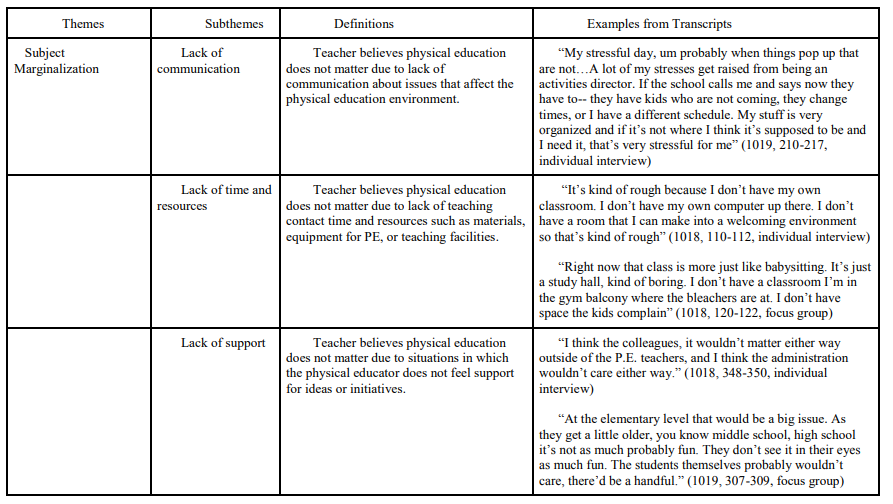
\includegraphics[width=\maxwidth{.95\linewidth}]{gfx/08-codebook}
	\caption{Example Codebook}
	\label{fig08.02}
\end{figure}

Data entry is the part of the survey where the data collected are entered into a computer for analysis. Most surveys are conducted online or using electronic devices like tablets so the data are already in digital format. It is also possible to use a data capture form that can be scanned into a computer. However, data that are collected using simple ``paper and pencil'' forms must be manually entered into a computer for analysis. This is a time consuming and, frankly, boring task that researchers must simply slog through before beginning analysis.

After the data are in a digital format then there are several good tools researchers can use for analysis. Quantitative data can be analyzed with \textit{R}, \textit{SPSS}, or \textit{Excel}. Of these tools, \textit{Excel} is the one most students are familiar with but its application for research statistical analysis is somewhat limited. \textit{SPSS} is very powerful but expensive. \textit{R} is available as a free download, is very powerful, but has a rather steep learning curve. 

Once the data are coded into a computer they must be analyzed. One of the simplest type of analysis is to look for patterns in the data. \Gls{univariate} analysis is the most basic form of quantitative analysis and involves finding patterns across just one variable. For \gls{continuousdata}, analysis tools include the central measure, histograms, and box plots. For \gls{discretedata}, analysis tools include frequency distributions and bar plots. \Gls{bivariate} analysis looks for relationships between two variables and analysis tools include correlations and scatter plots. Multivariate analysis looks for relationships between three or more variables. 

Another common method of data analysis is hypothesis testing. In this case, researchers have postulated a \gls{hypothesis} and then conduct research to either support or refute the hypothesis. Any of the pattern-finding tools mentioned in the previous paragraph can be used for hypothesis testing, but other more powerful tools are also available, like an \gls{anova} or Kruskal-Wallis H.

\subsection{Biases in Survey Research}

Despite all of its strengths and advantages, survey research is often tainted with systematic \glspl{bias} that may invalidate some of the inferences derived from such surveys. Five such biases are the non-response bias, sampling bias, social desirability bias, recall bias, and common method bias.

\begin{description}
	\item[Non-response bias]\label{08:nonresponse} Survey research is generally notorious for its low response rates. A response rate of $ 15-20\% $ is typical in a mail survey, even after two or three reminders. If the majority of the targeted respondents fail to respond to a survey, then a legitimate concern is whether non-respondents are not responding due to a systematic reason, which may raise questions about the validity of the study's results. For instance, dissatisfied customers tend to be more vocal about their experience than satisfied customers, and are therefore more likely to respond to questionnaire surveys or interview requests than satisfied customers. Hence, any respondent sample is likely to have a higher proportion of dissatisfied customers than the underlying population from which it is drawn. In this instance, not only will the results lack generalizability, but the observed outcomes may also be an artifact of the biased sample. The following strategies may be employed to improve response rates.

\begin{itemize}
	\item \textbf{Advance notification}. A short letter sent in advance to the targeted respondents soliciting their participation in an upcoming survey can prepare them in advance and improve their propensity to respond. The letter should state the purpose and importance of the study, mode of data collection (\eg, via a phone call, a survey form in the mail, etc.), and appreciation for their cooperation. A variation of this technique may request the respondent to return a postage-paid postcard indicating whether or not they are willing to participate in the study.

	\item \textbf{Relevance of content}. Respondents are more likely to respond to a survey that they consider relevant or important than to ones that do not matter.

	\item \textbf{Respondent-friendly questionnaire} Shorter survey questionnaires tend to elicit higher response rates than longer questionnaires. Furthermore, questions that are clear, non-offensive, and easy to respond to tend to attract higher response rates.

	\item \textbf{Endorsement}. For organizational surveys, it helps to gain the endorsement from a senior executive attesting to the importance of the study to the organization. Such endorsement can be in the form of a cover letter or a letter of introduction, which can improve the researcher's credibility in the eyes of the respondents.

	\item \textbf{Follow-up requests}. Multiple follow-up requests may coax some non-respondents to respond, even if their responses are late.

	\item \textbf{Interviewer training} Response rates for interviews can be improved with skilled interviewers trained on how to request interviews, use computerized dialing techniques to identify potential respondents, and schedule callbacks for respondents who could not be reached.

	\item \textbf{Incentives} Response rates, at least with certain populations, may increase with the use of incentives in the form of cash or gift cards, giveaways such as pens or stress balls, entry into a lottery, draw or contest, discount coupons, promise of contribution to charity, and so forth.

	\item \textbf{Non-monetary incentives} Businesses, in particular, are more prone to respond to non-monetary incentives than financial incentives. An example of such a non-monetary incentive is a bench marking report comparing the business's individual response against the aggregate of all responses to a survey.

	\item \textbf{Confidentiality and privacy}. Finally, assurances that the respondent's private data or responses will not fall into the hands of any third party may help improve response rates.
\end{itemize}

\item[Sampling bias] Bias can be introduced in a poorly-designed survey by using the wrong sample selection. Telephone surveys conducted by calling a random sample of publicly available mobile phone numbers will systematically exclude people with who do not own a mobile phone, and people who are unable to answer the phone (for instance, they are at work) when the survey is being conducted, and will include a disproportionate number of respondents who have who stay home during much of the day, such as the unemployed, the disabled, and the elderly. Likewise, online surveys tend to include a disproportionate number of students and younger people who are constantly on the Internet, and systematically exclude people with limited or no access to computers or the Internet, such as the poor and the elderly. Similarly, questionnaire surveys tend to exclude children and the illiterate, who are unable to read, understand, or meaningfully respond to the questionnaire. A different kind of sampling bias relate to sampling the wrong population, such as asking teachers (or parents) about academic learning of their students (or children), or asking CEOs about operational details in their company. Such biases make the respondent sample unrepresentative of the intended population and call into question generalizability claims about inferences drawn from the biased sample.

\item[Social desirability bias] Many respondents tend to avoid negative opinions or embarrassing comments about themselves, their employers, family, or friends. With negative questions such as ``do you think that your project team is dysfunctional,'' the researcher may not get truthful responses. This tendency among respondents to ``spin the truth'' in order to portray themselves in a socially desirable manner is called the ``social desirability bias,'' which hurts the validity of response obtained from survey research. There is practically no way of overcoming the social desirability bias in a questionnaire survey, but in an interview setting, an astute interviewer may be able to spot inconsistent answers and ask probing questions or use personal observations to supplement respondents' comments.

\item[Recall bias] Responses to survey questions often depend on subjects' motivation, memory, and ability to respond. Particularly when dealing with events that happened in the distant past, respondents may not adequately remember their own motivations or behaviors or perhaps their memory of such events may have evolved with time and no longer retrievable. For instance, if respondents are asked to describe their utilization of computer technology one year ago or even memorable childhood events like birthdays, their response may not be accurate due to difficulties with recall. One possible way of overcoming the recall bias is by anchoring respondent's memory in specific events as they happened, rather than asking them to recall their perceptions and motivations from memory.

\item[Common method bias] Common method bias refers to the amount of spurious covariance shared between independent and dependent variables that are measured at the same point in time, such as in a cross-sectional survey, using the same instrument, such as a questionnaire. In such cases, the phenomenon under investigation may not be adequately separated from measurement artifacts. This bias can be potentially avoided if the independent and dependent variables are measured at different points in time, using a longitudinal survey design, of if these variables are measured using different methods, such as computerized recording of dependent variable versus questionnaire-based self-rating of independent variables.

\end{description}

\section{Summary}

\begin{center}
	\begin{tkawybox}{Summary}
		\begin{itemize}
			\setlength{\itemsep}{0pt}
			\setlength{\parskip}{0pt}
			\setlength{\parsep}{0pt}
			
			\item Differentiate between cross-sectional and longitudinal surveys
			\item Compare and contrast the four types of longitudinal surveys: trend, panel, cohort, and retrospective
			\item Describe the characteristics of effective questions
			\item Define the various question response options
			\item Describe tips for creating good questionnaires
			\item Discuss how survey data are analyzed
			\item Discuss bias in survey research

		\end{itemize}
	\end{tkawybox}
\end{center}

%%*****************************************
\chapter{Experimental Research}\label{ch10:experimental_research}
%*****************************************
%TODO Status: Pre-draft

\section{Blackstone: Experiments}
% page 154

\begin{center}
	\begin{objbox}{Objectives}
		\begin{itemize}
			\setlength{\itemsep}{0pt}
			\setlength{\parskip}{0pt}
			\setlength{\parsep}{0pt}
			
			\item Define experiment.
			\item Distinguish “true” experiments from preexperimental designs.
			\item Identify the core features of true experimental designs.
			\item Describe the difference between an experimental group and a control group.
			\item Identify and describe the various types of true experimental designs.
			\item Identify and describe the various types of preexperimental designs.
			\item Name the key strengths and weaknesses of experiments.
			\item Define internal validity and external validity.
			
		\end{itemize}
	\end{objbox}
\end{center}

Experiments are an excellent data collection strategy for those wishing to observe the consequences of very specific actions or stimuli. Most commonly a quantitative research method, experiments are used more often by psychologists than sociologists, but understanding what experiments are and how they are conducted is useful for all social scientists, whether they actually plan to use this methodology or simply aim to understand findings based on experimental designs. An experiment is a method of data collection designed to test hypotheses under controlled conditions. Students in my research methods classes often use the term experiment to describe all kinds of empirical research projects, but in social scientific research, the term has a unique meaning and should not be used to describe all research methodologies.

Several kinds of experimental designs exist. In general, designs considered to be “true experiments” contain three key features: independent and dependent variables, pretesting and posttesting, and experimental and control groups. In the classic experiment, the effect of a stimulus is tested by comparing two groups: one that is exposed to the stimulus (the experimental group) and another that does not receive the stimulus (the control group). In other words, the effects of an independent variable upon a dependent variable are tested. Because the researcher’s interest lies in the effects of an independent variable, she must measure participants on the dependent variable before and after the independent variable (or stimulus) is administered. Thus pretesting and posttesting are both important steps in a classic experiment.

One example of experimental research can be found in Shannon K. McCoy and Brenda Major’s (2003) [1] study of people’s perceptions of prejudice. In one portion of this multifaceted study, all participants were given a pretest to assess their levels of depression. No significant differences in depression were found between the experimental and control groups during the pretest. Participants in the experimental group were then asked to read an article suggesting that prejudice against their own racial group is severe and pervasive, while participants in the control group were asked to read an article suggesting that prejudice against a racial group other than their own is severe and pervasive. Upon measuring depression scores during the posttest period, the researchers discovered that those who had received the experimental stimulus (the article citing prejudice against their same racial group) reported greater depression than those in the control group. This is just one of many examples of social scientific experimental research.

In addition to the classic experimental design, there are two other ways of designing experiments that are considered to fall within the purview of “true” experiments (Babbie, 2010; Campbell \& Stanley, 1963). [2] They are the Solomon four-group design and the posttest-only control group design. In the former, four groups exist. Two groups are treated as they would be in a classic experiment. Another group receives the stimulus and is then given the posttest. The remaining group does not receive the stimulus but is given the posttest. Table 12.2 "Solomon Four-Group Design" illustrates the features of each of the four groups in the Solomon four-group design.

Table: Solomon Four-Group Design

Finally, the posttest only control group is also considered a “true” experimental design though it lacks any pretest group. In this design, participants are assigned to either an experimental or a control group. Individuals are then measured on some dependent variable following the administration of an experimental stimulus to the experimental group. In theory, as long as the control and experimental groups have been determined randomly, no pretest is needed.

Time, other resources such as funding, and even one’s topic may limit a researcher’s ability to conduct a true experiment. For researchers in the medical and health sciences, conducting a true experiment could require denying needed treatment to patients, which is a clear ethical violation. Even those whose research may not involve the administration of needed medications or treatments may be limited in their ability to conduct a classic experiment. In social scientific experiments, for example, it might not be equitable or ethical to provide a large financial or other reward only to members of the experimental group. When random assignment of participants into experimental and control groups is not feasible, researchers may turn to a preexperimental design (Campbell \& Stanley, 1963). [3] However, this type of design comes with some unique disadvantages, which we’ll describe as we review the preexperimental designs available.

If we wished to measure the impact of some natural disaster, for example, Hurricane Katrina, we might conduct a preexperiment by identifying an experimental group from a community that experienced the hurricane and a control group from a similar community that had not been hit by the hurricane. This study design, called a static group comparison, has the advantage of including a comparison control group that did not experience the stimulus (in this case, the hurricane) but the disadvantage of containing experimental and control groups that were determined by a factor or factors other than random assignment. As you might have guessed from our example, static group comparisons are useful in cases where a researcher cannot control or predict whether, when, or how the stimulus is administered, as in the case of natural disasters.

In cases where the administration of the stimulus is quite costly or otherwise not possible, a one-shot case study design might be used. In this instance, no pretest is administered, nor is a control group present. In our example of the study of the impact of Hurricane Katrina, a researcher using this design would test the impact of Katrina only among a community that was hit by the hurricane and not seek out a comparison group from a community that did not experience the hurricane. Researchers using this design must be extremely cautious about making claims regarding the effect of the stimulus, though the design could be useful for exploratory studies aimed at testing one’s measures or the feasibility of further study.

Finally, if a researcher is unlikely to be able to identify a sample large enough to split into multiple groups, or if he or she simply doesn’t have access to a control group, the researcher might use a one-group pre-/posttest design. In this instance, pre- and posttests are both taken but, as stated, there is no control group to which to compare the experimental group. We might be able to study of the impact of Hurricane Katrina using this design if we’d been collecting data on the impacted communities prior to the hurricane. We could then collect similar data after the hurricane. Applying this design involves a bit of serendipity and chance. Without having collected data from impacted communities prior to the hurricane, we would be unable to employ a one-group pre-/posttest design to study Hurricane Katrina’s impact.

Table: Preexperimental Designs

As implied by the preceding examples where we considered studying the impact of Hurricane Katrina, experiments do not necessarily need to take place in the controlled setting of a lab. In fact, many applied researchers rely on experiments to assess the impact and effectiveness of various programs and policies. You might recall our discussion of the police experiment described in Chapter 2 "Linking Methods With Theory". It is an excellent example of an applied experiment. Researchers did not “subject” participants to conditions in a lab setting; instead, they applied their stimulus (in this case, arrest) to some subjects in the field and they also had a control group in the field that did not receive the stimulus (and therefore were not arrested).

Finally, a review of some of the strengths and weaknesses of experiments as a method of data collection is in order. A strength of this method, particularly in cases where experiments are conducted in lab settings, is that the researcher has substantial control over the conditions to which participants are subjected. Experiments are also generally easier to replicate than are other methods of data collection. Again, this is particularly true in cases where an experiment has been conducted in a lab setting.

As sociologists, who are especially attentive to how social context shapes social life, are likely to point out, a disadvantage of experiments is that they are rather artificial. How often do real-world social interactions occur in the same way that they do in a lab? Experiments that are conducted in applied settings may not be as subject to artificiality, though then their conditions are less easily controlled. Experiments also present a few unique concerns regarding validity. Problems of external validity might arise when the conditions of an experiment don’t adequately represent those of the world outside the boundaries of the experiment. In the case of McCoy and Major’s (2003) [4] research on prejudice described earlier in this section, for example, the questions to ask with regard to external validity are these: Can we say with certainty that the stimulus applied to the experimental group resembles the stimuli that people are likely to encounter in their real lives outside of the lab? Will reading an article on prejudice against one’s race in a lab have the same impact that it would outside of the lab? This is not to suggest that experimental research is not or cannot be valid, but experimental researchers must always be aware that external validity problems can occur and be forthcoming in their reports of findings about this potential weakness. Concerns about internal validity also arise in experimental designs. These have to do with our level of confidence about whether the stimulus actually produced the observed effect or whether some other factor, such as other conditions of the experiment or changes in participants over time, may have produced the effect.

In sum, the potential strengths and weaknesses of experiments as a method of data collection in social scientific research include the following:

Table: Strengths and Weaknesses of Experimental Research

\paragraph{Key Takeaways}

\begin{itemize}
	\setlength{\itemsep}{0pt}
	\setlength{\parskip}{0pt}
	\setlength{\parsep}{0pt}
	
	\item Experiments are designed to test hypotheses under controlled conditions.
	\item True experimental designs differ from preexperimental designs.
	\item Preexperimental designs each lack one of the core features of true experimental designs.
	\item Experiments enable researchers to have great control over the conditions to which participants are subjected and are typically easier to replicate than other methods of data collection.
	\item Experiments come with some degree of artificiality and may run into problems of external or internal validity.
	
\end{itemize}

\section{Anol: Experimental Research}
% Page 92 of her book

Experimental research, often considered to be the “gold standard” in research designs, is one of the most rigorous of all research designs. In this design, one or more independent variables are manipulated by the researcher (as treatments), subjects are randomly assigned to different treatment levels (random assignment), and the results of the treatments on outcomes (dependent variables) are observed. The unique strength of experimental research is its internal validity (causality) due to its ability to link cause and effect through treatment manipulation, while controlling for the spurious effect of extraneous variable.

Experimental research is best suited for explanatory research (rather than for descriptive or exploratory research), where the goal of the study is to examine cause-effect relationships. It also works well for research that involves a relatively limited and well-defined set of independent variables that can either be manipulated or controlled. Experimental research can be conducted in laboratory or field settings. Laboratory experiments, conducted in laboratory (artificial) settings, tend to be high in internal validity, but this comes at the cost of low external validity (generalizability), because the artificial (laboratory) setting in which the study is conducted may not reflect the real world. Field experiments, conducted in field settings such as in a real organization, and high in both internal and external validity. But such experiments are relatively rare, because of the difficulties associated with manipulating treatments and controlling for extraneous effects in a field setting.

Experimental research can be grouped into two broad categories: true experimental designs and quasi-experimental designs. Both designs require treatment manipulation, but while true experiments also require random assignment, quasi-experiments do not. Sometimes, we also refer to non-experimental research, which is not really a research design, but an all-inclusive term that includes all types of research that do not employ treatment manipulation or random assignment, such as survey research, observational research, and correlational studies.

\subsection{Basic Concepts}

\paragraph{Treatment and control groups.} In experimental research, some subjects are administered one or more experimental stimulus called a treatment (the treatment group) while other subjects are not given such a stimulus (the control group). The treatment may be considered successful if subjects in the treatment group rate more favorably on outcome variables than control group subjects. Multiple levels of experimental stimulus may be administered, in which case, there may be more than one treatment group. For example, in order to test the effects of a new drug intended to treat a certain medical condition like dementia, if a sample of dementia patients is randomly divided into three groups, with the first group receiving a high dosage of the drug, the second group receiving a low dosage, and the third group receives a placebo such as a sugar pill (control group), then the first two groups are experimental groups and the third group is a control group. After administering the drug for a period of time, if the condition of the experimental group subjects improved significantly more than the control group subjects, we can say that the drug is effective. We can also compare the conditions of the high and low dosage experimental groups to determine if the high dose is more effective than the low dose.

\paragraph{Treatment manipulation.} Treatments are the unique feature of experimental research that sets this design apart from all other research methods. Treatment manipulation helps control for the “cause” in cause-effect relationships. Naturally, the validity of experimental research depends on how well the treatment was manipulated. Treatment manipulation must be checked using pretests and pilot tests prior to the experimental study. Any measurements conducted before the treatment is administered are called pretest measures, while those conducted after the treatment are posttest measures. 

\paragraph{Random selection and assignment.} Random selection is the process of randomly drawing a sample from a population or a sampling frame. This approach is typically employed in survey research, and assures that each unit in the population has a positive chance of being selected into the sample. Random assignment is however a process of randomly assigning subjects to experimental or control groups. This is a standard practice in true experimental research to ensure that treatment groups are similar (equivalent) to each other and to the control group, prior to treatment administration. Random selection is related to sampling, and is therefore, more closely related to the external validity (generalizability) of findings. However, random assignment is related to design, and is therefore most related to internal validity. It is possible to have both random selection and random assignment in well-designed experimental research, but quasi-experimental research involves neither random selection nor random assignment.

\paragraph{Threats to internal validity.} Although experimental designs are considered more rigorous than other research methods in terms of the internal validity of their inferences (by virtue of their ability to control causes through treatment manipulation), they are not immune to internal validity threats. Some of these threats to internal validity are described below, within the context of a study of the impact of a special remedial math tutoring program for improving the math abilities of high school students.

\begin{itemize}
	\item \textit{History threat} is the possibility that the observed effects (dependent variables) are caused by extraneous or historical events rather than by the experimental treatment. For instance, students’ post-remedial math score improvement may have been caused by their preparation for a math exam at their school, rather than the remedial math program.
	\item \textit{Maturation threat} refers to the possibility that observed effects are caused by natural maturation of subjects (e.g., a general improvement in their intellectual ability to understand complex concepts) rather than the experimental treatment.
	\item \textit{Testing threat} is a threat in pre-post designs where subjects’ posttest responses are conditioned by their pretest responses. For instance, if students remember their answers from the pretest evaluation, they may tend to repeat them in the posttest exam. Not conducting a pretest can help avoid this threat.
	\item \textit{Instrumentation threat}, which also occurs in pre-post designs, refers to the possibility that the difference between pretest and posttest scores is not due to the remedial math program, but due to changes in the administered test, such as the posttest having a higher or lower degree of difficulty than the pretest.
	\item \textit{Mortality threat} refers to the possibility that subjects may be dropping out of the study at differential rates between the treatment and control groups due to a systematic reason, such that the dropouts were mostly students who scored low on the pretest. If the low-performing students drop out, the results of the posttest will be artificially inflated by the preponderance of high-performing students.
	\item \textit{Regression threat}, also called a regression to the mean, refers to the statistical tendency of a group’s overall performance on a measure during a posttest to regress toward the mean of that measure rather than in the anticipated direction. For instance, if subjects scored high on a pretest, they will have a tendency to score lower on the posttest (closer to the mean) because their high scores (away from the mean) during the pretest was possibly a statistical aberration. This problem tends to be more prevalent in nonrandom samples and when the two measures are imperfectly correlated.
\end{itemize}

\subsection{Two-Group Experimental Designs}

The simplest true experimental designs are two group designs involving one treatment group and one control group, and are ideally suited for testing the effects of a single independent variable that can be manipulated as a treatment. The two basic two-group designs are the pretest-posttest control group design and the posttest-only control group design, while variations may include covariance designs. These designs are often depicted using a standardized design notation, where R represents random assignment of subjects to groups, X represents the treatment administered to the treatment group, and O represents pretest or posttest observations of the dependent variable (with different subscripts to distinguish between pretest and posttest observations of treatment and control groups).

\paragraph{Pretest-posttest control group design.} In this design, subjects are randomly assigned to treatment and control groups, subjected to an initial (pretest) measurement of the dependent variables of interest, the treatment group is administered a treatment (representing the independent variable of interest), and the dependent variables measured again (posttest). The notation of this design is shown in Figure 10.1.

Figure 10.1. Pretest-posttest control group design

The effect E of the experimental treatment in the pretest posttest design is measured as the difference in the posttest and pretest scores between the treatment and control groups:

E = (O2 – O1) – (O4 – O3)

Statistical analysis of this design involves a simple analysis of variance (ANOVA) between the treatment and control groups. The pretest posttest design handles several threats to internal validity, such as maturation, testing, and regression, since these threats can be expected to influence both treatment and control groups in a similar (random) manner. The selection threat is controlled via random assignment. However, additional threats to internal validity may exist. For instance, mortality can be a problem if there are differential dropout rates between the two groups, and the pretest measurement may bias the posttest measurement (especially if the pretest introduces unusual topics or content).

\paragraph{Posttest-only control group design.} This design is a simpler version of the pretestposttest design where pretest measurements are omitted. The design notation is shown in Figure 10.2.

Figure 10.2. Posttest only control group design

The treatment effect is measured simply as the difference in the posttest scores between the two groups:

E = (O1 – O2)

The appropriate statistical analysis of this design is also a two-group analysis of variance (ANOVA). The simplicity of this design makes it more attractive than the pretestposttest design in terms of internal validity. This design controls for maturation, testing, regression, selection, and pretest-posttest interaction, though the mortality threat may continue to exist.

\paragraph{Covariance designs.} Sometimes, measures of dependent variables may be influenced by extraneous variables called covariates. Covariates are those variables that are not of central interest to an experimental study, but should nevertheless be controlled in an experimental design in order to eliminate their potential effect on the dependent variable and therefore allow for a more accurate detection of the effects of the independent variables of interest. The experimental designs discussed earlier did not control for such covariates. A covariance design (also called a concomitant variable design) is a special type of pretest posttest control group design where the pretest measure is essentially a measurement of the covariates of interest rather than that of the dependent variables. The design notation is shown in Figure 10.3, where C represents the covariates:

Figure 10.3. Covariance design

Because the pretest measure is not a measurement of the dependent variable, but rather a covariate, the treatment effect is measured as the difference in the posttest scores between the treatment and control groups as:

E = (O1 – O2)

Due to the presence of covariates, the right statistical analysis of this design is a twogroup analysis of covariance (ANCOVA). This design has all the advantages of post-test only design, but with internal validity due to the controlling of covariates. Covariance designs can also be extended to pretest-posttest control group design.

\subsection{Factorial Designs}

Two-group designs are inadequate if your research requires manipulation of two or more independent variables (treatments). In such cases, you would need four or higher-group designs. Such designs, quite popular in experimental research, are commonly called factorial designs. Each independent variable in this design is called a factor, and each sub-division of a factor is called a level. Factorial designs enable the researcher to examine not only the individual effect of each treatment on the dependent variables (called main effects), but also their joint effect (called interaction effects).

The most basic factorial design is a 2 x 2 factorial design, which consists of two treatments, each with two levels (such as high/low or present/absent). For instance, let’s say that you want to compare the learning outcomes of two different types of instructional techniques (in-class and online instruction), and you also want to examine whether these effects vary with the time of instruction (1.5 or 3 hours per week). In this case, you have two factors: instructional type and instructional time; each with two levels (in-class and online for instructional type, and 1.5 and 3 hours/week for instructional time), as shown in Figure 8.1. If you wish to add a third level of instructional time (say 6 hours/week), then the second factor will consist of three levels and you will have a 2 x 3 factorial design. On the other hand, if you wish to add a third factor such as group work (present versus absent), you will have a 2 x 2 x 2 factorial design. In this notation, each number represents a factor, and the value of each factor represents the number of levels in that factor.

Figure 10.4. 2 x 2 factorial design

Factorial designs can also be depicted using a design notation, such as that shown on the right panel of Figure 10.4. R represents random assignment of subjects to treatment groups, X represents the treatment groups themselves (the subscripts of X represents the level of each factor), and O represent observations of the dependent variable. Notice that the 2 x 2 factorial design will have four treatment groups, corresponding to the four combinations of the two levels of each factor. Correspondingly, the 2 x 3 design will have six treatment groups, and the 2 x 2 x 2 design will have eight treatment groups. As a rule of thumb, each cell in a factorial design should have a minimum sample size of 20 (this estimate is derived from Cohen’s power calculations based on medium effect sizes). So a 2 x 2 x 2 factorial design requires a minimum total sample size of 160 subjects, with at least 20 subjects in each cell. As you can see, the cost of data collection can increase substantially with more levels or factors in your factorial design. Sometimes, due to resource constraints, some cells in such factorial designs may not receive any treatment at all, which are called incomplete factorial designs. Such incomplete designs hurt our ability to draw inferences about the incomplete factors.

In a factorial design, a main effect is said to exist if the dependent variable shows a significant difference between multiple levels of one factor, at all levels of other factors. No change in the dependent variable across factor levels is the null case (baseline), from which main effects are evaluated. In the above example, you may see a main effect of instructional type, instructional time, or both on learning outcomes. An interaction effect exists when the effect of differences in one factor depends upon the level of a second factor. In our example, if the effect of instructional type on learning outcomes is greater for 3 hours/week of instructional time than for 1.5 hours/week, then we can say that there is an interaction effect between instructional type and instructional time on learning outcomes. Note that the presence of interaction effects dominate and make main effects irrelevant, and it is not meaningful to interpret main effects if interaction effects are significant.

\subsection{Hybrid Experimental Designs}

Hybrid designs are those that are formed by combining features of more established designs. Three such hybrid designs are randomized bocks design, Solomon four-group design, and switched replications design.

\paragraph{Randomized block design.} This is a variation of the posttest-only or pretest-posttest control group design where the subject population can be grouped into relatively homogeneous subgroups (called blocks) within which the experiment is replicated. For instance, if you want to replicate the same posttest-only design among university students and full-time working professionals (two homogeneous blocks), subjects in both blocks are randomly split between treatment group (receiving the same treatment) or control group (see Figure 10.5). The purpose of this design is to reduce the “noise” or variance in data that may be attributable to differences between the blocks so that the actual effect of interest can be detected more accurately.

Figure 10.5. Randomized blocks design

\paragraph{Solomon four-group design.} In this design, the sample is divided into two treatment groups and two control groups. One treatment group and one control group receive the pretest, and the other two groups do not. This design represents a combination of posttest-only and pretest-posttest control group design, and is intended to test for the potential biasing effect of pretest measurement on posttest measures that tends to occur in pretest-posttest designs but not in posttest only designs. The design notation is shown in Figure 10.6.

Figure 10.6. Solomon four-group design

\paragraph{Switched replication design.} This is a two-group design implemented in two phases with three waves of measurement. The treatment group in the first phase serves as the control group in the second phase, and the control group in the first phase becomes the treatment group in the second phase, as illustrated in Figure 10.7. In other words, the original design is repeated or replicated temporally with treatment/control roles switched between the two groups. By the end of the study, all participants will have received the treatment either during the first or the second phase. This design is most feasible in organizational contexts where organizational programs (e.g., employee training) are implemented in a phased manner or are repeated at regular intervals.

Figure 10.7. Switched replication design

\subsection{Quasi-Experimental Designs}

Quasi-experimental designs are almost identical to true experimental designs, but lacking one key ingredient: random assignment. For instance, one entire class section or one organization is used as the treatment group, while another section of the same class or a different organization in the same industry is used as the control group. This lack of random assignment potentially results in groups that are non-equivalent, such as one group possessing greater mastery of a certain content than the other group, say by virtue of having a better teacher in a previous semester, which introduces the possibility of selection bias. Quasiexperimental designs are therefore inferior to true experimental designs in interval validity due to the presence of a variety of selection related threats such as selection-maturation threat (the treatment and control groups maturing at different rates), selection-history threat (the treatment and control groups being differentially impact by extraneous or historical events), selection-regression threat (the treatment and control groups regressing toward the mean between pretest and posttest at different rates), selection-instrumentation threat (the treatment and control groups responding differently to the measurement), selection-testing (the treatment and control groups responding differently to the pretest), and selectionmortality (the treatment and control groups demonstrating differential dropout rates). Given these selection threats, it is generally preferable to avoid quasi-experimental designs to the greatest extent possible.

Many true experimental designs can be converted to quasi-experimental designs by omitting random assignment. For instance, the quasi-equivalent version of pretest-posttest control group design is called nonequivalent groups design (NEGD), as shown in Figure 10.8, with random assignment R replaced by non-equivalent (non-random) assignment N. Likewise, the quasi-experimental version of switched replication design is called non-equivalent switched replication design (see Figure 10.9).

Figure 10.8. NEGD design

Figure 10.9. Non-equivalent switched replication design

In addition, there are quite a few unique non-equivalent designs without corresponding true experimental design cousins. Some of the more useful of these designs are discussed next.

\paragraph{Regression-discontinuity (RD) design.} This is a non-equivalent pretest-posttest design where subjects are assigned to treatment or control group based on a cutoff score on a preprogram measure. For instance, patients who are severely ill may be assigned to a treatment group to test the efficacy of a new drug or treatment protocol and those who are mildly ill are assigned to the control group. In another example, students who are lagging behind on standardized test scores may be selected for a remedial curriculum program intended to improve their performance, while those who score high on such tests are not selected from the remedial program. The design notation can be represented as follows, where C represents the cutoff score:

Figure 10.10. RD design

Because of the use of a cutoff score, it is possible that the observed results may be a function of the cutoff score rather than the treatment, which introduces a new threat to internal validity. However, using the cutoff score also ensures that limited or costly resources are distributed to people who need them the most rather than randomly across a population, while simultaneously allowing a quasi-experimental treatment. The control group scores in the RD design does not serve as a benchmark for comparing treatment group scores, given the systematic non-equivalence between the two groups. Rather, if there is no discontinuity between pretest and posttest scores in the control group, but such a discontinuity persists in the treatment group, then this discontinuity is viewed as evidence of the treatment effect.

\paragraph{Proxy pretest design.} This design, shown in Figure 10.11, looks very similar to the standard NEGD (pretest-posttest) design, with one critical difference: the pretest score is collected after the treatment is administered. A typical application of this design is when a researcher is brought in to test the efficacy of a program (e.g., an educational program) after the program has already started and pretest data is not available. Under such circumstances, the best option for the researcher is often to use a different prerecorded measure, such as students’ grade point average before the start of the program, as a proxy for pretest data. A variation of the proxy pretest design is to use subjects’ posttest recollection of pretest data, which may be subject to recall bias, but nevertheless may provide a measure of perceived gain or change in the dependent variable.

Figure 10.11. Proxy pretest design

\paragraph{Separate pretest-posttest samples design.} This design is useful if it is not possible to collect pretest and posttest data from the same subjects for some reason. As shown in Figure 10.12, there are four groups in this design, but two groups come from a single non-equivalent group, while the other two groups come from a different non-equivalent group. For instance, you want to test customer satisfaction with a new online service that is implemented in one city but not in another. In this case, customers in the first city serve as the treatment group and those in the second city constitute the control group. If it is not possible to obtain pretest and posttest measures from the same customers, you can measure customer satisfaction at one point in time, implement the new service program, and measure customer satisfaction (with a different set of customers) after the program is implemented. Customer satisfaction is also measured in the control group at the same times as in the treatment group, but without the new program implementation. The design is not particularly strong, because you cannot examine the changes in any specific customer’s satisfaction score before and after the implementation, but you can only examine average customer satisfaction scores. Despite the lower internal validity, this design may still be a useful way of collecting quasi-experimental data when pretest and posttest data are not available from the same subjects.

Figure 10.12. Separate pretest-posttest samples design

\paragraph{Nonequivalent dependent variable (NEDV) design.} This is a single-group pre-post quasi-experimental design with two outcome measures, where one measure is theoretically expected to be influenced by the treatment and the other measure is not. For instance, if you are designing a new calculus curriculum for high school students, this curriculum is likely to influence students’ posttest calculus scores but not algebra scores. However, the posttest algebra scores may still vary due to extraneous factors such as history or maturation. Hence, the pre-post algebra scores can be used as a control measure, while that of pre-post calculus can be treated as the treatment measure. The design notation, shown in Figure 10.13, indicates the single group by a single N, followed by pretest O1 and posttest O2 for calculus and algebra for the same group of students. This design is weak in internal validity, but its advantage lies in not having to use a separate control group.

An interesting variation of the NEDV design is a pattern matching NEDV design, which employs multiple outcome variables and a theory that explains how much each variable will be affected by the treatment. The researcher can then examine if the theoretical prediction is matched in actual observations. This pattern-matching technique, based on the degree of correspondence between theoretical and observed patterns is a powerful way of alleviating internal validity concerns in the original NEDV design.

Figure 10.13. NEDV design

\subsection{Perils of Experimental Research}

Experimental research is one of the most difficult of research designs, and should not be taken lightly. This type of research is often best with a multitude of methodological problems. First, though experimental research requires theories for framing hypotheses for testing, much of current experimental research is atheoretical. Without theories, the hypotheses being tested tend to be ad hoc, possibly illogical, and meaningless. Second, many of the measurement instruments used in experimental research are not tested for reliability and validity, and are incomparable across studies. Consequently, results generated using such instruments are also incomparable. Third, many experimental research use inappropriate research designs, such as irrelevant dependent variables, no interaction effects, no experimental controls, and nonequivalent stimulus across treatment groups. Findings from such studies tend to lack internal validity and are highly suspect. Fourth, the treatments (tasks) used in experimental research may be diverse, incomparable, and inconsistent across studies and sometimes inappropriate for the subject population. For instance, undergraduate student subjects are often asked to pretend that they are marketing managers and asked to perform a complex budget allocation task in which they have no experience or expertise. The use of such inappropriate tasks,  introduces new threats to internal validity (i.e., subject’s performance may be an artifact of the content or difficulty of the task setting), generates findings that are non-interpretable and meaningless, and makes integration of findings across studies impossible.

The design of proper experimental treatments is a very important task in experimental design, because the treatment is the raison d’etre of the experimental method, and must never be rushed or neglected. To design an adequate and appropriate task, researchers should use prevalidated tasks if available, conduct treatment manipulation checks to check for the adequacy of such tasks (by debriefing subjects after performing the assigned task), conduct pilot tests (repeatedly, if necessary), and if doubt, using tasks that are simpler and familiar forthe respondent sample than tasks that are complex or unfamiliar.

In summary, this chapter introduced key concepts in the experimental design research method and introduced a variety of true experimental and quasi-experimental designs. Although these designs vary widely in internal validity, designs with less internal validity should not be overlooked and may sometimes be useful under specific circumstances and empirical contingencies.





\section{Summary}\label{ch10:summary}

Lorem ipsum dolor sit amet, consectetuer adipiscing elit. Aenean commodo ligula eget dolor. Aenean massa. Cum sociis natoque penatibus et


\ctparttext{Qualitative methods are based in the evaluation of non-numeric data, like photographs and text documents. These methods include activities like field work, unobtrusive, and interpretive research methods.}
\part{Qualitative Methods}
\cleardoublepage
%%*****************************************
\chapter{Interviews}\label{ch10:interviews}
%*****************************************
%TODO Status: Pre-draft

\section{What Is Interview Research?}

\begin{wrapfigure}{r}{0.4\textwidth}
	\centering
	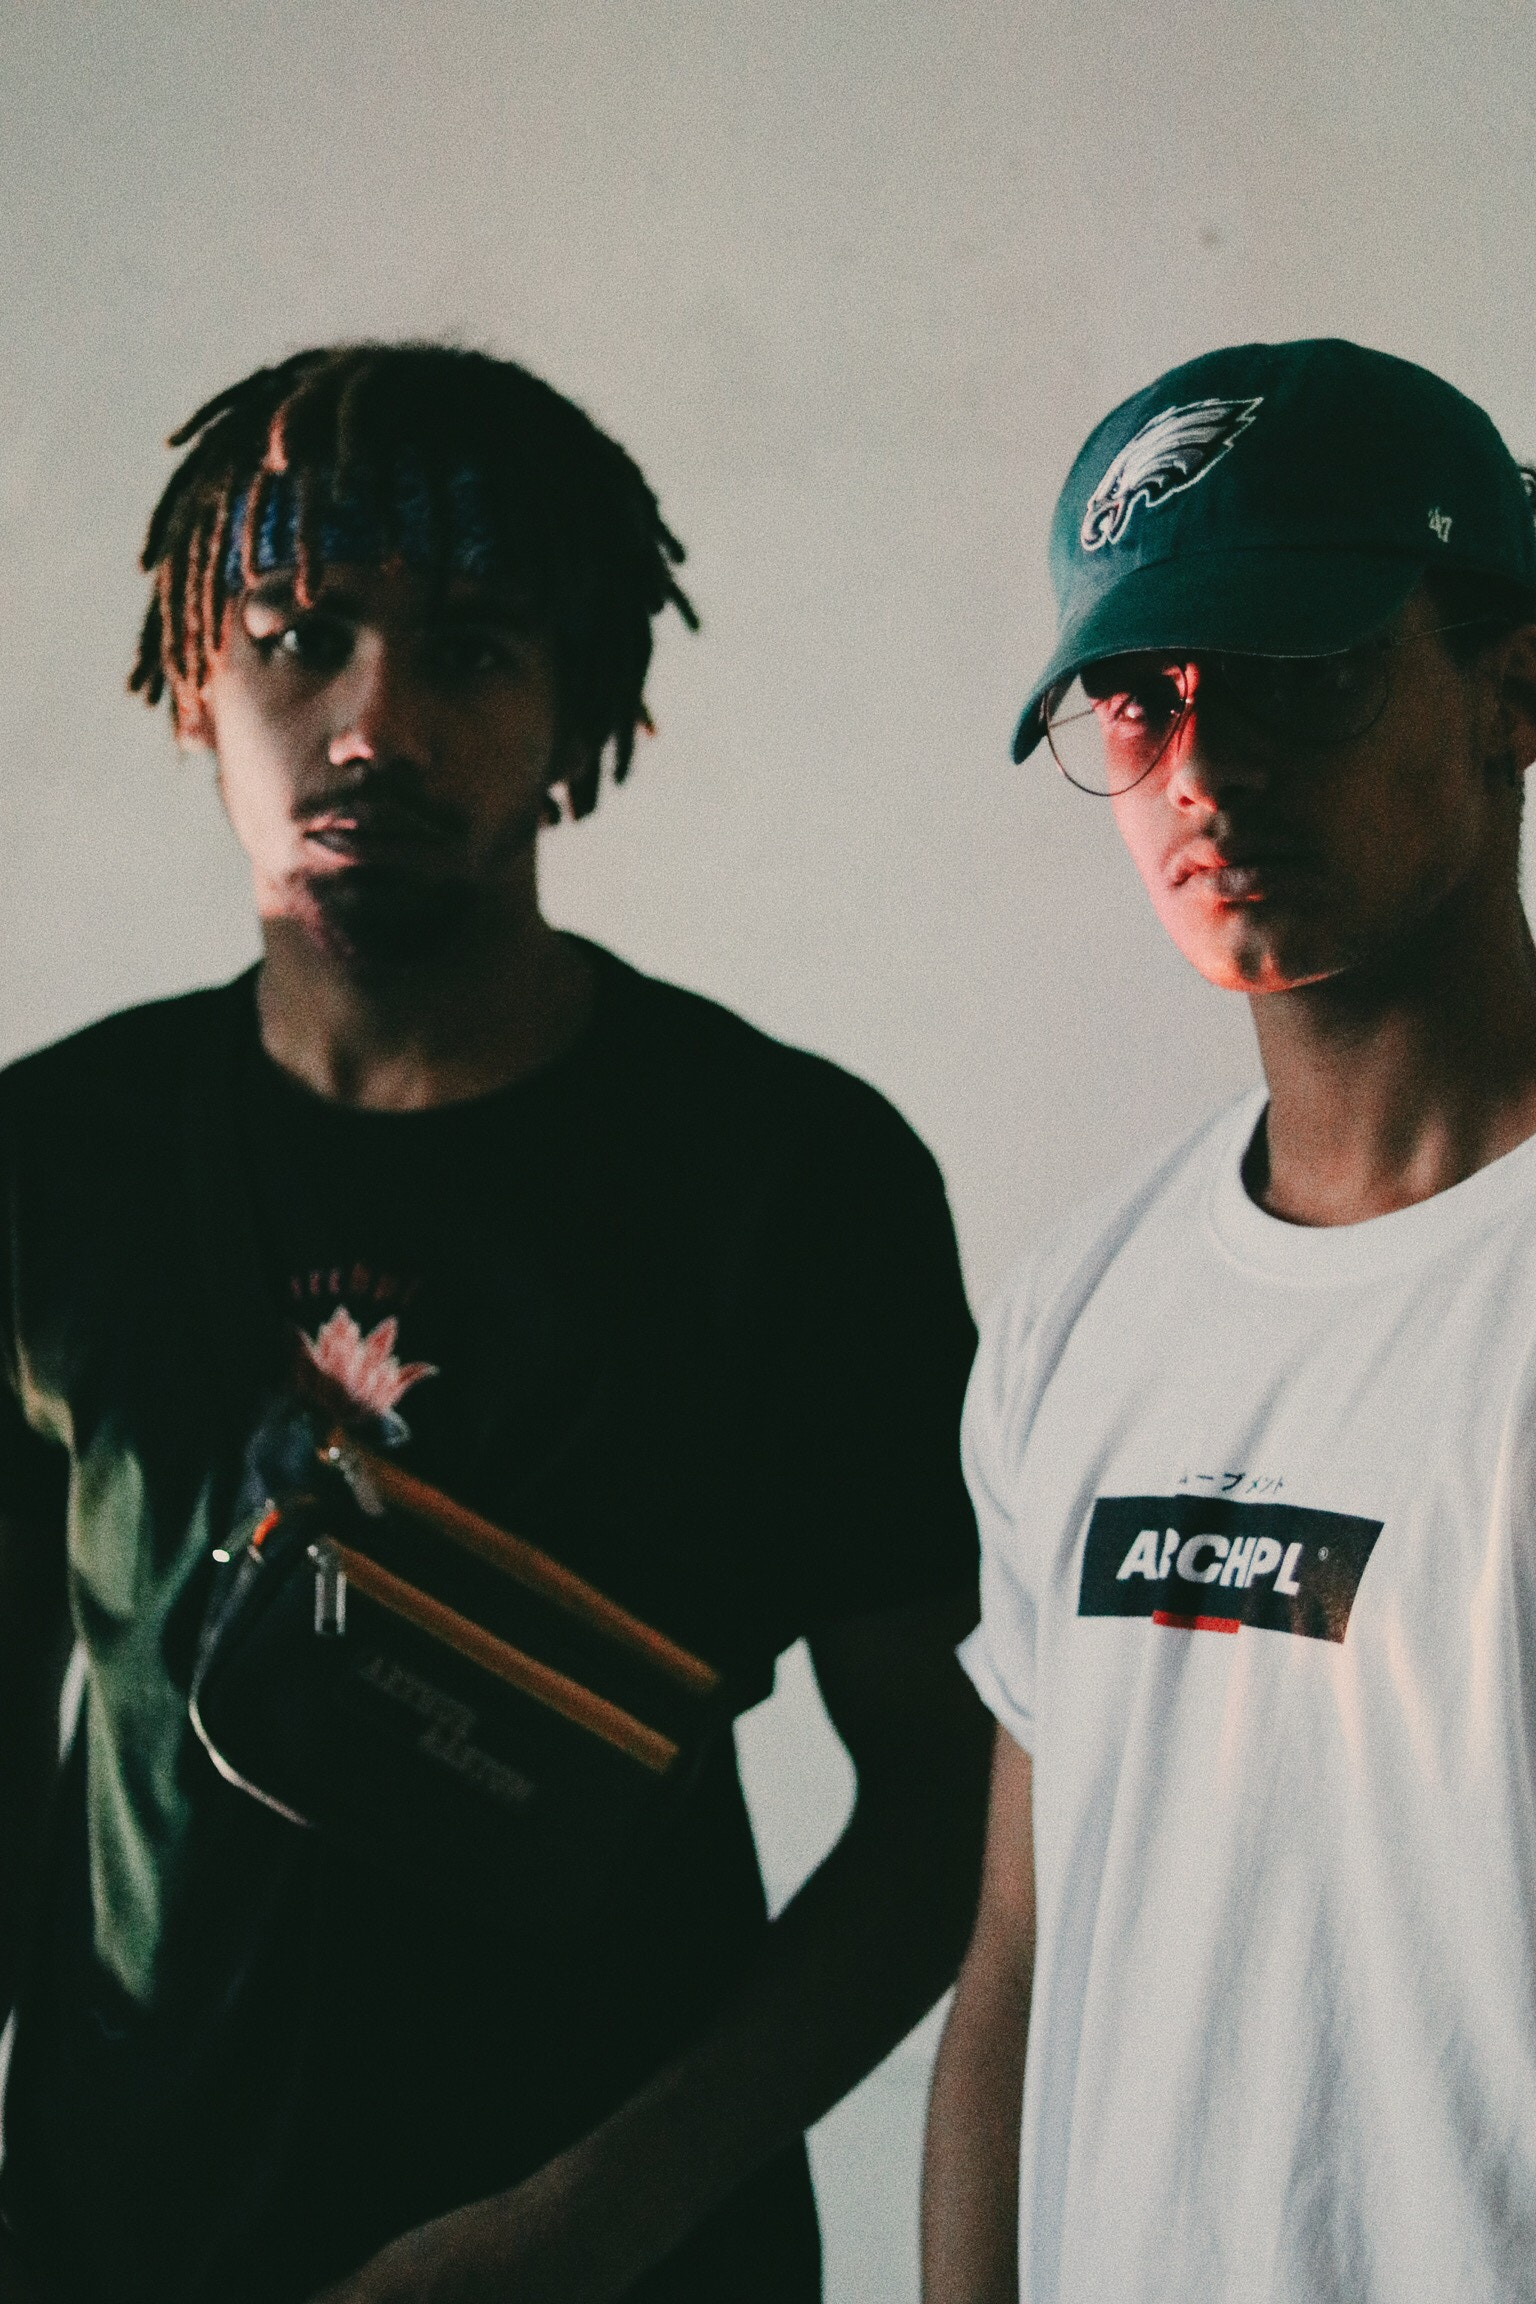
\includegraphics[width=0.4\textwidth]{gfx/09-men} 
\end{wrapfigure}

Today's young men are delaying their entry into adulthood. That's a nice way of saying they are ``totally confused;'' ``cannot commit to their relationships, work, or lives;'' and are ``obsessed with never wanting to grow up.''\footnote{All of the quotes in the first paragraph were found at \url{http://guyland.net/}.} But don't take my word for it. Take sociologist Michael Kimmel's word. He interviewed $ 400 $ young men, ages $ 16 $ to $ 26 $, over the course of four years across the United States to learn how they made the transition from adolescence into adulthood. Since the results of Kimmel's research were published in $ 2008 $ \cite{kimmel2008perilous} his work has made quite a splash. Featured in news reports, on blogs, and in many book reviews, some claim Kimmel's research ``could save the humanity of many young men.'' Whatever is correct about Kimmel's research, one thing remains true: We surely would not know nearly as much as we now do about the lives of many young American men were it not for interview research.\footnote{Photo by Tom Cochereau on Unsplash}

Knowing how to create and conduct a good interview is an essential skill for researchers, especially those interested in \gls{qualitativeresearch}. Interviews are used by market researchers to learn how to sell their products, journalists use interviews to get information from a whole host of people from VIPs to random people on the street. Television interviewers help viewers get to know guests on their shows, employers use them to make decisions about job offers, and even radio hosts interview call-in participants. It seems everyone who's anyone knows how to conduct an interview.

From the research perspective, interviews are a method of data collection that involves two or more people exchanging information through a series of questions and answers. The questions are designed by a researcher to elicit information from interview participant(s) on a specific topic or set of topics. Typically interviews involve an in-person meeting between two people, an interviewer and an interviewee. But interviews need not be limited to two people nor must they occur in person.

Interviews are an excellent way to gather detailed information. They also have an advantage over surveys; with a survey, if a participant's response sparks some follow-up question, researchers generally do not have an opportunity to ask for more information. What they get is what they get. so to speak. In an interview, however, because researchers are actually talking with the study participants in real time, they can ask follow-up questions and help clarify the responses. Thus, interviews are a useful method to find out the ``story'' behind the responses in a written survey.

Interviews are also useful when the research topic is rather complex, when the question being asked requires explanation, or when the answers to the questions may not be immediately clear to participants who may need some time in order to work through their responses. Also, if the research topic is one about which people will likely have a lot to say or will want to provide some explanation or describe some process, interviews may be the best method. 

In sum, interview research is especially useful when the following are true:

\begin{enumerate}
	\item very detailed information is requested
	\item it is anticipated that respondents will need to be asked for more information about their responses
	\item the questions require lengthy explanation
	\item the topic is complex or may be confusing to respondents
	\item the involves studying processes
\end{enumerate}

\subsection{Role of the Interviewer}

The interviewer has a complex and multi-faceted role in the interview process, which includes the following tasks:

\begin{itemize}
	\item \textbf{Prepare for the interview}. Since the interviewer is in the forefront of the data collection effort, the quality of data collected depends heavily on how well the interviewer is trained to do the job. The interviewer must be trained in the interview process and the survey method, and also be familiar with the purpose of the study, how responses will be stored and used, and sources of interviewer bias. Interviewers should also rehearse and time the interview prior to the formal study.
	\item \textbf{Locate and enlist the cooperation of respondents}. Particularly in cases where the interview will take place in the participant's home, the interviewer must locate the address and work around respondents' schedule, sometimes at undesirable times such as weekends. They should also be like a salesperson and ``sell'' the idea of participating in the study.
	\item \textbf{Motivate respondents}. Respondents often feed off the motivation of the interviewer. If the interviewer is disinterested or inattentive, respondents will not be motivated to provide useful or informative responses. The interviewer must demonstrate enthusiasm about the study, communicate the importance of the research to respondents, and be attentive to respondents' needs throughout the interview. 
	\item \textbf{Clarify any confusion or concerns}. Interviewers must be able to think on their feet and address unanticipated concerns or objections raised by respondents. Additionally, they should ask probing questions as necessary even if such questions are not in the script.
	\item \textbf{Observe quality of response}. The interviewer is in the best position to judge the quality of information collected, and may supplement verbal responses obtained by also recording personal observations of gestures and body language.
\end{itemize}

\section{Qualitative Interview Techniques}

Qualitative interviews are sometimes called ``intensive'' or ``in-depth'' interviews. These interviews are semistructured where researchers will have a particular topic for the interview, but questions are open ended and may not be asked in exactly the same way or in exactly the same order to each respondent. During qualitative interviews, the primary aim is to hear from respondents about what they think is important and to hear it in their own words. This section considers conducting qualitative interviews, analyzing interview data, and the strengths and weaknesses of this method.

\subsection{Conducting Qualitative Interviews}

Qualitative interviews might feel more like a conversation than an interview to respondents, but the researcher is in fact usually guiding the conversation with the goal of gathering information on a specific topic from a respondent. A key difference between qualitative and quantitative interviewing is that qualitative interviews are semi-structured and contain open-ended questions where quantitative interviews are structured and contain close-ended questions. Open-ended questions are more demanding of participants than closed-ended questions since they require participants to come up with their own words, phrases, or sentences to respond.

In a qualitative interview, researchers usually use a guide, which is a list of topics or questions to be covered during the interview. It is called a ``guide'' because it is simply that---it is used to \textit{guide} the interview, but it is not set in stone. Think of an interview guide like an agenda for a meeting, it contains the goals to be accomplished but it is not critical if an item is skipped or if the order is changed somewhat. 

Interview guides outline issues that are important, but because participants are asked to provide answers in their own words, and to raise points that they believe are important, each interview is likely to flow a little differently. While the opening question in an in-depth interview may be the same across all interviews, from that point on what the participant says will shape how the interview proceeds. Many researchers believe that this free flow of topics makes in-depth interviewing exciting. It is also what makes in-depth interviewing rather challenging to conduct. It takes a skilled interviewer to be able to ask questions, listen to respondents, and pick up on cues about when to follow up, when to move on, and when to simply let the participant speak without guidance or interruption.

Interview guides tend to list topics or even specific questions, but the format of an interview guide might depend on the researcher's style, experience, and comfort level as an interviewer or with the topic. For example, in interviews of young people about their experiences with workplace sexual harassment, the guide may be topic-based with few specific questions contained in the guide. Instead, it could contain only an outline of topics that are important for the research, listed in an order that it might make sense to cover them, noted on a sheet of paper.

Of course, interview guides do not appear out of thin air. They are the result of thoughtful and careful work on the part of a researcher. The topics and questions are organized thematically and in the order in which they are likely to proceed, though the flow of a qualitative interview is in part determined by what a respondent has to say. Sometimes qualitative interviewers may create two versions of the interview guide, one version contains a very brief outline of the interview, perhaps with just topic headings, and another version contains detailed questions underneath each topic heading. In this case, the researcher might use the very detailed guide to prepare and practice in advance of actually conducting interviews and then just bring the brief outline to the interview. Bringing an outline, as opposed to a very long list of detailed questions, to an interview encourages the researcher to actually listen to what the participant is saying. An overly detailed interview guide will be difficult to navigate through during an interview and could give respondents the impression that the interviewer is more interested in the questions than in the participant's answers.

Brainstorming is a good first step in constructing an interview guide. There are no rules at the brainstorming stage---simply list all the topics and questions that come to mind when thinking about the research question. Once a good list is created, it can be pared down by cutting questions and topics that seem redundant and grouping like questions and topics together. It is at this point that headings for grouped categories are developed. Another important avenue of approach is to consult scholarly literature to find out what kinds of questions other interviewers have asked in similar studies. As with quantitative survey research, it is best not to place very sensitive or potentially controversial questions at the very beginning of the qualitative interview guide. Participants need the opportunity to warm up to the interview and to feel comfortable talking with the interviewer. Finally, it is important to get feedback on the interview guide as it is being developed. Researchers should ask peers for guidance and suggestions once they come up with what they think is a pretty strong guide. Chances are that peer reviewers will find ways to improve the guide.

There are a few guidelines worth noting about the specific questions in the guide.

\begin{itemize}
	\item Avoid questions that can be answered with a simple yes or no. 
	\item If yes/no questions must be asked, include follow-up questions. One of the benefits of qualitative interviews is that participants can be asked for more information.
	\item While follow-up questions are appropriate, ``why'' should be avoided since this particular question can be construed as confrontational. Instead of ``why,'' something like, ``Could you tell me a little more about that?'' is a good option.
	\item Leading questions should be avoided. For example, rather than asking, ``Don't you agree that people who spend money frivolously are selfish?'' ask ``What comes to mind when you hear that someone has spent money frivolously?''
	\item Keep most, if not all, questions open ended. The key to a successful qualitative interview is giving participants the opportunity to share information in their own words and in their own way.
\end{itemize}

After the interview guide is constructed, the interviewer is still not ready to begin conducting interviews. The researcher next has to decide how to collect and maintain the information that is provided by participants. 

It is probably most common for qualitative interviewers to take audio recordings of the interviews they conduct. Recording interviews allows researchers to focus on their interaction with the interview participant rather than being distracted by trying to take notes. Of course, not all participants will feel comfortable being recorded and sometimes even the interviewer may feel that the subject is so sensitive that recording would be inappropriate. If this is the case, it is up to the researcher to balance note-taking with listening. 

Practicing the interview in advance is crucial. Ideally, researchers should interview one or two peers, or even friends, who are willing to participate in trial runs. Even better are a few people who are similar in at least some ways to the sample. The trial runs can provide feedback on the questions and the demeanor of the interviewer.

\subsection{Analysis of Qualitative Interview Data}

Analysis of qualitative interview data typically begins with a set of transcripts of the interviews. Ideally, researchers who recorded the interview can have the recordings transcribed so a written verbatim record is available. Interviewers who relied on notes taken during the interview should write a full version of the notes as quickly as possible after the interview while the session is still fresh in mind. It is usually helpful to also note non-verbal items such as body language, tone of voice, or unusually long pauses before an answer.  

While third party transcribers are easily found, it may be best for the interviewer to transcribe the recordings personally. Often, things can be recalled and noted about nonverbal behaviors and interactions that may be relevant to analysis but that could not be picked up by the audio recording alone. For example, interviewees may roll their eyes, wipe tears from their face, and even make obscene gestures that speak volumes about their feelings but would have been lost if the interviewer had not transcribed the recording personally.

The goal of analysis is to reach some inferences, lessons, or conclusions by condensing large amounts of data into relatively smaller, more manageable bits of understandable information. Analysis of qualitative interview data is normally \gls{inductiveresearch} and moves from the specific observations an interviewer collects to identifying patterns across those observations. Qualitative interviewers typically begin by reading through transcripts of their interviews and identifying codes, which is a shorthand representation of some complex set of issues or ideas. This phase of the research is often referred to as ``coding'' and it involves reading and rereading (and rereading again) all of the interview transcripts until the researcher has a clear idea about what sorts of themes come up across the interviews.

Qualitative researcher and textbook author Kristin Esterberg \cite{esterberg2002qualitative} describes coding as a multistage process. She suggests that there are two types of coding: open coding and focused coding. To analyze qualitative interview data, researchers can begin by open coding transcripts. They read through each transcript, line by line, and make a note of whatever categories or themes emerge. At this stage, it is important that they not let the original research question or expectations about what they think they may find cloud their ability to see new categories or themes. This is called open coding for a reason, they must keep an open mind. Open coding usually requires multiple go-rounds. As they read through the transcripts, they begin to see commonalities across the categories or themes. Then, they can begin focused coding.

Focused coding involves collapsing or narrowing themes and categories identified in open coding by reading through the notes made while conducting open coding. Researchers identify themes or categories that seem to be related, perhaps merging some or redefining others. Then they give each theme or category a name or code. Then, they identify passages of data that represent the emerging codes by reading through the transcripts yet again (and probably again). They also might write up brief definitions or descriptions of each code to making meaning of the data and develop a way to talk about the findings.

As tedious and laborious as it might seem to read through hundreds of pages of transcripts multiple times, sometimes getting started with the coding process is actually the hardest part. In their text on analyzing qualitative data, Lofland and Lofland \cite{lofland1995analytic} identify a set of questions that may be useful when coding qualitative data.

\begin{enumerate}
	\item Of what topic, unit, or aspect is this an instance?
	\item What question about a topic does this item of data suggest?
	\item What sort of answer to a question about a topic does this item of data suggest (i.e., what proposition is suggested)?
\end{enumerate}

Qualitative data can be analyzed with tools like \textit{NVivo}, \textit{RQDA}, and \textit{Coding Analysis Toolkit}\footnote{NVivo information can be found at \url{http://www.qsrinternational.com}, RQDA at \url{http://rqda.r-forge.r-project.org/}, and Coding Analysis Toolkit at \url{https://cat.texifter.com/}}. \textit{NVivo} is very powerful but expensive. \textit{RQDA} is an \textit{R} package that is useful for qualitative data analysis. Since it is part of the \textit{R} system it could be easily used in a mixed methods project where \textit{R} is used for quantitative and \textit{RQDA} is used for qualitative analysis. \textit{Coding Analysis Toolkit} is a free online text analysis service. These programs are specifically designed to assist qualitative researchers with organizing, managing, sorting, and analyzing large amounts of qualitative data. The programs work by allowing researchers to import interview transcripts and then label or code passages, cut and paste passages, search for various words or phrases, and organize complex interrelationships among passages and codes.

As an example, the following excerpt, from a paper analyzing the electronic gaming industry in two jurisdictions, \cite{buchanan2010efficacy} summarizes how the process of analyzing qualitative interview data often works.

\begin{quote}
	Data were collected through these combined methods, and while analysis was undertaken using NVivo, the analysis was guided by these methods. Thirty-eight in-depth interviews were undertaken with gaming operators and gaming machine manufacturers in both the Nevada (USA) and NSW (Australian) jurisdictions during $ 2005-2006 $. Interview data were augmented through observation, resulting in a rich collection of data. The data were coded and initially entered into ‘nodes’ within the NVivo program. A pre-defined set of themes was derived from topic areas of the interviews. Each theme then became a node. As each interview was read, additional themes were identified and nodes created for each theme. The nodes were fleshed out as data were extracted from each interview referring to the same theme. Thus a range of themes was created as a result of going through the data and coding according to themes within each transcript. Once all data had been placed into various nodes, themes were checked through the matrix function within NVivo to ensure that the various themes were distinct from each other and that there was no redundancy. 
	
	Further analysis of emerging themes resulted in a conceptual model\ldots
\end{quote}

\subsection{Strengths and Weaknesses of Qualitative Interviews}

As the preceding sections have suggested, qualitative interviews are an excellent way to gather detailed information. Whatever topic is of interest to researchers employing this method can be explored in much more depth than with almost any other method. Not only are participants given the opportunity to elaborate in a way that is not possible with other methods like survey research, but they also are able share information with researchers in their own words and from their own perspectives rather than being asked to fit those perspectives into limited response options provided by the researcher. Because qualitative interviews are designed to elicit detailed information, they are especially useful when a researcher's aim is to study processes, or the ``how'' of various phenomena. Yet another, and sometimes overlooked, benefit of qualitative interviews that it occurs in person so researchers can make observations beyond those that a respondent is orally reporting. A respondent's body language, and even her or his choice of time and location for the interview, might provide a researcher useful data.

Of course, all these benefits do not come without some drawbacks. As with quantitative survey research, qualitative interviews rely on respondents' ability to accurately and honestly recall whatever details about their lives, circumstances, thoughts, opinions, or behaviors are being asked about. Further, qualitative interviewing is time intensive and can be quite expensive. Creating an interview guide, identifying a sample, and conducting interviews are just the beginning. Transcribing interviews is labor intensive---and that's before coding even begins. It is also not uncommon to offer respondents some monetary incentive or thank-you for participating since researchers are asking for more of the participants' time than if they had simply mailed them a questionnaire. Conducting qualitative interviews is not only labor intensive but also potentially emotionally taxing. It may be that the researcher will hear stories that are shocking, infuriating, and sad.  Researchers embarking on a qualitative interview project should keep in mind their own abilities to hear stories that may be difficult to hear.

\section{Quantitative Interview Techniques}

Quantitative interviews are similar to qualitative interviews in that they involve some researcher/respondent interaction. But the process of conducting and analyzing findings from quantitative interviews differs in several ways from that of qualitative interviews. Each approach also comes with its own unique set of strengths and weaknesses.

\subsection{Conducting Quantitative Interviews}

Much of what was covered earlier in this chapter and in Chapter \ref{08:surveys}, page \pageref{08:surveys}, applies to quantitative interviews as well. In fact, quantitative interviews are sometimes referred to as ``survey interviews'' because they resemble survey-style question-and-answer formats. The difference between quantitative interviews and surveys is that in an interview questions and answer options are read to respondents rather than having respondents complete a questionnaire on their own. As with questionnaires, the questions posed in a standardized interview tend to be closed ended. There are instances in which a quantitative interviewer might pose a few open-ended questions as well. In these cases, the coding process works somewhat differently than coding in-depth interview data.

In quantitative interviews, an interview schedule is used to guide researchers as they pose questions and answer options to respondents. An interview schedule is usually more rigid than an interview guide. It contains the list of questions and answer options that the researcher will read to respondents. Whereas qualitative researchers emphasize respondents' roles in helping to determine how an interview progresses, in a quantitative interview, consistency in the way that questions and answer options are presented is very important. The aim is \textit{to pose every question-and-answer option in the very same way to every respondent}. This is done to minimize interviewer effect, or possible changes in the way an interviewee responds based on how or when questions and answer options are presented by the interviewer.

Quantitative interviews may be recorded, but because questions tend to be closed ended, taking notes during the interview is less disruptive than it can be during a qualitative interview. If a quantitative interview contains open-ended questions, however, recording the interview is advised. It may also be helpful to record quantitative interviews if a researcher wishes to assess possible interview effect. Noticeable differences in responses might be more attributable to interviewer effect than to any real respondent differences. Having a recording of the interview can help researchers make such determinations.

Quantitative interviewers are usually more concerned with gathering data from a large, representative sample but collecting data from many people via interviews can be quite laborious. Technological advances in telephone interviewing procedures can assist quantitative interviewers in this process. Random Digit Dialing (\textit{RDD}) programs call randomly generated phone numbers for researchers conducting phone interviews. Computer-assisted telephone interviewing (\textit{CATI}) programs can also aid quantitative survey researchers. These programs allow an interviewer to enter responses directly into a computer as they are provided, thus saving hours of time that would otherwise have to be spent entering data into an analysis program by hand. Also available are Automated Computer Telephone Interviewing (\textit{ACTI}) programs where a program generates questions with a realistic voice and then uses voice recognition to record responses. Unfortunately, due to the pervasive increase in ``push polling'' for election campaigns, many respondents are unwilling to speak to a researcher on the phone.

\subsection{Analysis of Quantitative Interview Data}

As with the analysis of survey data, analysis of quantitative interview data usually involves coding response options numerically, entering numeric responses into a data analysis computer program, and then running various statistical commands to identify patterns across responses. Chapter \ref{08:surveys}, Section \ref{08:analysisOfSurveyData}, \nameref{08:analysisOfSurveyData}, page \pageref{08:analysisOfSurveyData}, describes the coding process for quantitative data. But what happens when quantitative interviews ask open-ended questions? In this case, responses are typically numerically coded, just as closed-ended questions are, but the process is a little more complex than simply giving a ``no'' a label of $ 0 $ and a ``yes'' a label of $ 1 $.

In some cases, quantitatively coding open-ended interview questions may work inductively. If this is the case, rather than ending with codes, descriptions of codes, and interview excerpts, the researcher will assign a numerical value to codes and may not utilize verbatim excerpts from interviews in later reports of results. Keep in mind that with quantitative methods the aim is to be able to represent and condense data into numbers. The quantitative coding of open-ended interview questions is often a deductive process. The researcher may begin with an idea about likely responses to his or her open-ended questions and assign a numerical value to each likely response. Then researchers will review participants' open-ended responses and assign the numerical value that most closely matches the value of their expected response.

\subsection{Strengths and Weaknesses of Quantitative Interviews}

The strengths and weakness of quantitative interviews tend to be couched in comparison to those of administering hard copy questionnaires. For example, response rates tend to be higher with interviews than with mailed questionnaires. That makes sense---most people find it easier to say ``no'' to a piece of paper than to a person. Quantitative interviews can also help reduce respondent confusion. If a respondent is unsure about the meaning of a question or answer option on a questionnaire, he or she probably will not have the opportunity to get clarification from the researcher. An interview, on the other hand, gives the researcher an opportunity to clarify or explain any items that may be confusing.

As with every method of data collection, there are also drawbacks to conducting quantitative interviews. Perhaps the largest, and of most concern to quantitative researchers, is interviewer effect. While questions on hard copy questionnaires may create an impression based on the way they are presented, having a person administer questions introduces a slew of additional variables that might influence a respondent. Consistency is key with quantitative data collection---and human beings are not necessarily known for their consistency. Interviewing respondents is also much more time consuming and expensive than mailing questionnaires. Thus quantitative researchers may opt for written questionnaires over interviews on the grounds that they will be able to reach a large sample at a much lower cost than were they to interact personally with each and every respondent.

\section{Issues to Consider}
%TODO Start Here
While quantitative interviews resemble survey research in their question/answer formats, they share with qualitative interviews the characteristic that researchers actually interact with their subjects. The fact that researchers interacts with their subjects creates a few complexities that deserve attention.

\subsection{Power}

First and foremost, interviewers must be aware of and attentive to the power differential between themselves and interview participants. The interviewer sets the agenda and leads the conversation. While qualitative interviewers aim to allow participants to have some control over which or to what extent various topics are discussed, at the end of the day it is the researcher who is in charge (at least that is how most respondents will perceive the dynamic). Researcher are asking people to reveal things about themselves they may not typically share with others. Moreover, researchers are generally not reciprocating by revealing much or anything about themselves. All these factors shape the power dynamics of an interview.

A number of excellent pieces have been written dealing with issues of power in research and data collection. Anyan \cite{anyan2013influence} offered several suggestions for overcoming the power imbalance between researchers and participants during the data gathering phase, including the ``\ldots interviewer must court the interviewee, enhance the sense of rapport between them and build a sympathetic relationship and a sense of mutual trust in the research interview.'' During data analysis, researchers may want to consider letting interviewees interpret what they meant during the interview. ``The willingness to share the data analysis process with the interviewee or letting them join the final stages of writing is in the hands of the interviewer.'' However, researchers must be vigilant to not let the interviewee shape the outcome of the research project, researchers have an ethical obligation to maintain standards that the average interviewee would not understand.

Another easy way to balance the power differential between researchers and interview participants is to make the intent of the research project very clear. Sharing the rationale for conducting the research and the research question(s) that frame the project may help keep a proper balance of power. Participants should also understand how the data will be stored and used; and how their privacy will be protected. Many of these details are stipulated by the oversight group's procedures and requirements; but even if they are not, researchers should be attentive to how sharing information with participants can help balance the power differences between themselves and those who participate in the research project.

There are no easy answers when it comes to handling the power differential between the researcher and participants, and even professional researchers do not agree on the best approach for doing so. It is nevertheless an issue to be attentive to when conducting any form of research, particularly those that involve interpersonal interactions and relationships with research participants.

\subsection{Location}

One way to balance the power between researcher and respondent is to conduct the interview in a location of the participants' choosing, where they will feel most comfortable answering questions. Interviews can take place in any number of locations---in respondents' homes or offices, researchers' homes or offices, coffee shops, restaurants, public parks, or hotel lobbies, to name just a few possibilities. Each location comes with its own set of benefits and its own challenges. It may be best to allow the participant to choose the location that is most convenient and most comfortable, identifying a location where there will be few distractions is also important. For example, some coffee shops and restaurants are so loud that recording the interview can be a challenge. Other locations may present different sorts of distractions. For example, it may be that parents, out of necessity, will spend more time attending to their children during an interview than responding to questions. Interviewers should be prepared to suggest a few possible locations, and note the goal of avoiding distractions, when asking participants to choose a location.

Of course, the extent to which a respondent should be given complete control over choosing a location must also be balanced by accessibility of the location to the interviewer, and by the safety and comfort level of the location. It is conceivable, for example, that a participant's home could be decorated wall to wall with posters representing various white power organizations displaying a variety of violently racist messages. Even if the topic of the interview has nothing to do with home decor, the discomfort and fear the interviewer could feel during the interview could easily distracted from the task at hand. While it is important to conduct interviews in a location that is comfortable for respondents, doing so should never come at the expense of the interviewer's welfare or safety.

\subsection{Researcher-Respondent Relationship}

Finally, a unique feature of interviews is that they require social interaction, which means that to at least some extent, a relationship is formed between interviewer and interviewee. While there may be some differences in how the researcher-respondent relationship works depending on whether the interviews are qualitative or quantitative, one essential relationship element is the same: R-E-S-P-E-C-T. A good rapport between the interviewer and the participant is crucial to successful interviewing. Rapport is the sense of connection established between the interviewer and participant. Some argue that this term is too clinical and perhaps it implies that a researcher tricks a participant into thinking they are socially closer than they really are. While it is unfortunately true that some researchers might believe this implication, that is not the sense for rapport that researchers should attempt to establish with their subjects. Instead, as already mentioned, the key is \textit{respect}.

There are no big secrets or tricks for how to show respect for research participants. At its core, the interview interaction should not differ from any other social interaction in which interviewers show gratitude for a person's time and respect for a person's humanity. It is crucial that interviewers conduct the interview in a way that is culturally sensitive. In some cases, this might mean educating themselves about the study population and even receiving some training to help them learn to effectively communicate with the research participants. Interviewers should not judge participants; they are there to listen. Participants have been kind enough to give them their time and attention. Even if interviewers disagree strongly with what a participant shares in an interview, their job as researchers is to gather the information being shared, not to make personal judgments about it. 

Developing good rapport requires good listening. In fact, listening during an interview is an active, not a passive, practice. Active listening means that interviewers participate with the respondent by showing that they understand and follow whatever it is that is being shared. The questions asked to respondents should indicate that interviewers actually heard what they have just said. Active listening probably means that interviewers will probe the respondent for more information from time to time throughout the interview. A probe is a request for more information. Both qualitative and quantitative interviewers probe respondents, though the way they probe usually differs. In quantitative interviews, probing should be uniform. Often quantitative interviewers will predetermine what sorts of probes they will use. Interviewers should not to use probes that might appear to agree or disagree with what respondents said. So ``yes'' or ``I agree'' or even a questioning ``hmmmm'' should be avoided. Instead, responses like a simple ``thank you'' to indicate that the response was heard is more neutral. A ``yes'' or ``no'' response should be used if, and only if, a respondent specifically asks us if they were heard or understood.

In some ways qualitative interviews better lend themselves to following up with respondents and asking them to explain, describe, or otherwise provide more information. This is because qualitative interviewing techniques are designed to go with the flow and take whatever direction the respondent goes during the interview. Nevertheless, it is worth the interviewer's time to come up with helpful probes in advance of an interview even in the case of a qualitative interview. They do not want to find themselves stumped or speechless after a respondent has just said something about which needs to be probed further. This is another reason that practicing an interview in advance with people who are similar to those in the sample is a good idea.

\section{Conducting the Interview}

Before the interview, interviewers should prepare a ``kit'' to carry to the interview session, including a cover letter from the principal investigator or sponsor, adequate copies of the survey instrument, photo identification, and a telephone number for respondents to call to verify the interviewer's authenticity. The interviewer should set up an appointment and then be on time. To start the interview, interviewers should speak in an imperative and confident tone, such as ``I'd like to take a few minutes of your time to interview you for a very important study,'' instead of ``May I come in to do an interview?'' They should introduce themselves, present personal credentials, explain the purpose of the study in a few sentences, and assure confidentiality of respondents' comments, all in less than a minute. No big words or jargon should be used, and no details should be provided unless specifically requested. If interviewers wish to record the interview, they should ask for respondent's explicit permission before starting. Even if the interview is recorded, the interview must take notes on key issues, probes, or verbatim phrases.

During the interview, interviewers should follow the script and ask questions exactly as written. They should also not change the order of questions or skip any question that may have been answered earlier. Any issues with the questions should be discussed during rehearsal prior to the actual interview sessions. Interviewers should not finish the respondent's sentences. If the respondent gives a brief cursory answer, the interviewer should probe the respondent to elicit a more thoughtful, thorough response. Some useful probing techniques are:

\begin{itemize}
	\item \textbf{The silent probe}. Just pausing and waiting (without going into the next question) may suggest to respondents that the interviewer is waiting for more detailed response.
	\item \textbf{Overt encouragement}. Occasional ``uh-huh'' or ``okay'' may encourage the respondent to go into greater details. However, the interviewer must not express approval or disapproval of what was said by the respondent.
	\item \textbf{Ask for elaboration}. Such as ``can you elaborate on that?'' or ``A minute ago, you were talking about an experience you had in high school. Can you tell me more about that?''
	\item \textbf{Reflection}. Interviewers can try the psychotherapist's trick of repeating what the respondent said. For instance, ``What I'm hearing is that you found that experience very traumatic'' and then pause and wait for the respondent to elaborate.
\end{itemize}

After the interview in completed, interviewers should thank respondents for their time, tell them when to expect the results, and not leave hastily. Immediately after leaving, they should write down any notes or key observations that may help interpret the respondent's comments better.

\section{Focus Groups}

Focus groups resemble qualitative interviews in that a researcher may prepare an interview guide in advance and interact with participants by asking them questions. But anyone who has conducted both one-on-one interviews and focus groups knows that each is unique. In an interview, usually one member (the research participant) is most active while the other (the researcher) plays the role of listener, conversation guider, and question asker. Focus groups, on the other hand, are planned discussions designed to elicit group interaction and ``collects data through group interaction on a topic determined by the researcher.'' \cite{morgan1996focus} In this case, the researcher may play a less active role than in a one-on-one interview. The researcher's aim is to get participants talking to each other and to observe interactions among participants.

Focus groups are typically more dynamic than interviews. The researcher takes the role of moderator, posing questions or topics for discussion, but then lets the group members discuss the question or topic among themselves. Participants may ask each other follow-up questions, agree or disagree with one another, display body language that indicates something about their feelings, or even come up with questions not previously conceived of by the researcher. It is just these sorts of interactions and displays that are of interest to the researcher. A researcher conducting focus groups collects data on more than people's direct responses to her or his questions; the group interaction is a key focal point. Due to the nature and unpredictability of group interaction, and the fact that focus group researchers generally want to draw out group interaction, focus groups tend to be qualitative rather than quantitative.

There are numerous examples of marketing and business research using focus group methodology. 

In a $ 2009 $ study of the use of visual tobacco warnings, Gallopel-Morvan \etal. used focus groups and determined that the European Union graphic warnings on cigarette packages was more effective than text warnings. \cite{gallopel2011use} They used six focus group discussions conducted in Rennes, Paris, and Brest with a total of $ 50 $ people ($ 26 $ smokers, $ 24 $ non-smokers, $ 25 $ women, $ 25 $ men). 

An interesting study published by Wutich \etal in $ 2009 $ compared the results of a focus group with an open-ended self-administered questionnaire among water decision makers in Phoenix, Arizona. \cite{wutich2010comparing} She found that the focus group was no better than the questionnaires when the questions were only moderately sensitive, but the focus group was better ``\ldots for very sensitive topics when there appeared to be an opportunity to exchange important information or solve a pressing problem.''

In $ 2013 $, Sylvetsky \etal published the results of a focus group study where the effectiveness of advertising for the development of an obesity awareness campaign aimed at young people.  She conducted ten focus group discussions in two regions of Georgia, United States.  The groups of children, aged $ 9 - 14 $, were led in discussions concerning healthy food choice and lifestyles. They identified three themes: ``My Mom wants me to eat healthy foods like broccoli but it looks nasty and tastes gross,'' ``Obesity is a problem but is does not apply to me,'' and ``Everyone is made differently and it does not matter if you are fat.''

Government officials and political campaign workers use them to learn how members of the public feel about a particular issue or candidate. One of the earliest documented uses of focus groups comes from World War II when researchers used them to assess the effectiveness of troop training materials and of various propaganda efforts. \cite{merton1946focused} Market researchers quickly adopted this method of collecting data to learn about human beliefs and behaviors. Within social science, the use of focus groups did not really take off until the $ 1980 $s, when demographers and communication researchers began to appreciate their use in understanding knowledge, attitudes, and communication. Beyond various applied research projects, like those mentioned above, social scientists also use focus groups in theory development projects. 

Focus groups share many of the strengths and weaknesses of one-on-one qualitative interviews. Both methods can yield very detailed, in-depth information; are excellent for studying social processes; and provide researchers with an opportunity not only to hear what participants say but also to observe what they do in terms of their body language. Focus groups offer the added benefit of giving researchers a chance to collect data on human interaction by observing how group participants respond and react to one another. Like one-on-one qualitative interviews, focus groups can also be quite expensive and time-consuming. However, there may be some time savings with focus groups as it takes fewer group events than one-on-one interviews to gather data from the same number of people. Another potential drawback of focus groups, which is not a concern for one-on-one interviews, is that one or two participants might dominate the group, silencing other participants. Careful planning and skillful moderation on the part of the researcher are crucial for avoiding, or at least dealing with, such possibilities. The various strengths and weaknesses of focus group research are summarized below.

\begin{itemize}
	\item Strengths of Focus Group Research
	
	\begin{itemize}
		\item Yield detailed, in-depth data
		\item Less time-consuming than one-on-one interviews
		\item Useful for studying social processes
		\item Allow researchers to observe body language in addition to self-reports
		\item Allow researchers to observe interaction between multiple participants
	\end{itemize}
	
	\item Weaknesses of Focus Group Research
	
	\begin{itemize}
		\item Expensive
		\item May be more time-consuming than survey research
		\item Minority of participants may dominate entire group
	\end{itemize}
	
\end{itemize}

As mentioned, careful planning and skillful moderating are two crucial considerations in the effective use of focus groups as a method of data collection. In some ways, focus groups require more advance planning than other qualitative methods of data collection such as one-on-one interviews, where a researcher may be better able to control the setting and the dialogue, or field research, where ``going with the flow'' and observing events as they happen in their natural setting is the primary aim and time is less limited. Researchers must take care to form focus groups whose members will want to interact with one another and to control the timing of the event so that participants are not asked nor expected to stay for a longer time than they have agreed to participate. The researcher should also be prepared to inform focus group participants of their responsibility to maintain the confidentiality of what is said in the group. But while the researcher can and should encourage all focus group members to maintain confidentiality, she should also clarify to participants that the unique nature of the group setting prevents her from being able to promise that confidentiality will be maintained.

Group size should be determined in part by the topic of the interview and the researcher's sense of the likelihood that participants will have much to say without much prompting. If the topic is one about which the participants feel passionately and will have much to say, a group of three to five is ideal. Groups larger than that, especially for heated topics, can easily become unmanageable. Some recommend that a group of about six to ten participants is the ideal size for focus group research while others recommend that groups should include three to twelve participants. The size of the focus group is ultimately the researcher's decision. When forming groups and deciding how large or small to make them, researchers must take into consideration what they know about the topic and participants' potential interest in, passion for, and feelings about the topic. They must also consider their comfort level and experience in conducting focus groups. 

It may seem counterintuitive, but in general, it is better to form focus groups consisting of participants who do not know one another than to create groups consisting of friends, relatives, or acquaintances. The reason for this is that groups who know each other may share some take-for-granted knowledge or assumptions. In business research, it is precisely the taken-for-granted that is often of interest; thus the focus group researcher should avoid setting up interactions where participants may be discouraged to question or raise issues that they take for granted. However, groups should not be so heterogeneous that participants will be unlikely to feel comfortable talking with one another.

Focus group researchers must carefully consider the composition of the groups they put together. In his text on conducting focus groups, Morgan \cite{morgan1996focus} suggests that ``homogeneity in background and not homogeneity in attitudes'' should be the goal, since participants must feel comfortable speaking up but must also have enough differences to facilitate a productive discussion. Whatever composition researchers design for their focus groups, the important point to keep in mind is that focus group dynamics are shaped by multiple social contexts. Participants' silences as well as their speech may be shaped by gender, race, class, sexuality, age, or other background characteristics or social dynamics, all of which might be suppressed or exacerbated depending on the composition of the group.

In addition to the importance of advance planning, focus groups also require skillful moderation. While a researcher certainly does not want to be viewed as a stick-in-the-mud or as overly domineering, it is important to set ground rules for focus groups at the outset of the discussion. Participants should be reminded that they were invited to participate because the researcher wants to hear from all of them. Therefore, the group should aim to let just one person speak at a time and avoid letting just a couple of participants dominate the conversation. One way to do this is to begin the discussion by asking participants to briefly introduce themselves or to provide a brief response to an opening question. This will help set the tone of having all group members participate. Also ask participants to avoid having side conversations; sharing thoughts about or reactions to what is said in the group is important and should not be limited to only a few group members.

As the focus group gets rolling, the moderator will play a less active role than in a one-on-one interview. There may be times when the conversation stagnates or when the moderator wishes to guide the conversation in another direction. In these instances, it is important for moderators to demonstrate that they have been paying attention to what participants have said. Being prepared to interject statements or questions such as ``I'd really like to hear more about what Sally and Joe think about what Dominick and Ashley have been saying'' or ``Several of you have mentioned\ldots What do others think about this?'' will be important for keeping the conversation going. It can also help redirect the conversation, shift the focus to participants who have been less active in the group, and serve as a cue to those who may be dominating the conversation that it is time to allow others to speak.

In sum, focus groups are a useful method for researchers who wish to gather in-depth information about social processes. Focus groups are similar to one-on-one qualitative interviews in many ways, but they give researchers the opportunity to observe group dynamics that cannot be observed in one-on-one interviews. Historically, focus group research was more commonly used by applied researchers than by academics, though in recent decades social scientists from all domains have discovered the usefulness of focus groups for gaining understanding of social processes and have begun using this method of data collection in their studies.


\section{Summary}\label{ch10:summary}

Lorem ipsum dolor sit amet, consectetuer adipiscing elit. Aenean commodo ligula eget dolor. Aenean massa. Cum sociis natoque penatibus et

%%*****************************************
\chapter{Field Research}\label{ch11:field_research}
%*****************************************
%TODO Status: Pre-draft

\section{Introduction}

\begin{wrapfigure}{r}{0.4\textwidth}
	\centering
	
\includegraphics[width=0.4\textwidth]{gfx/11-mop} 
\end{wrapfigure}

If researchers wanted to know who conducts more of the housework in households, how could they find the answer? One way might be to interview people and simply ask them. That is exactly what Arlie Hochschild did in her study of the second shift, her term for the work that goes on in the home after the day's work for pay is completed\cite{hochschild2012second}. Hochschild interviewed $ 50 $ heterosexual, married couples with children to learn about how they did, or did not, share the work of the second shift. Many of these couples reported to her that they shared the load of the second shift equally, sometimes dividing the house into areas that were ``her responsibility'' and those that were ``his.'' But Hochschild was not satisfied with just people's personal accounts of second-shift work. She chose to observe $ 12 $ of these couples in their homes as well, to see for herself just how the second shift was shared.\blfootnote{Photo by rawpixel on Unsplash}

What Hochschild discovered was that even those couples who claimed to share the second shift did not have as equitable a division of duties as they had professed. For example, one couple who told Hochschild during their interview that they shared the household work equally had explained that the wife was responsible for the upstairs portion of the house and the husband took responsibility for the downstairs portion. Upon conducting observations in this couple's home, however, Hochschild discovered that the upstairs portion of the house contained all the bedrooms and bathrooms, the kitchen, the dining room, and the living room, while the downstairs included a storage space and the garage. This division of labor meant that the woman actually carried the weight of responsibility for the second shift. Without a field research component to her study, Hochschild might never have uncovered these and other truths about couples' behaviors and sharing (or not sharing) of household duties.

\begin{center}
	\begin{objbox}{Objectives}
		\begin{itemize}
			\setlength{\itemsep}{0pt}
			\setlength{\parskip}{0pt}
			\setlength{\parsep}{0pt}
			
			\item Define ``Field Research.''
			\item Describe the strengths and weaknesses of field research.
			\item Describe how to get started with field research: choosing a site and role.
			\item Describe how to write field notes and then analyze those notes.
		\end{itemize}
	\end{objbox}
\end{center}


\section{What Is Field Research?}

Field research is a qualitative method of data collection aimed at understanding, observing, and interacting with people in their natural settings. Thus when researchers talk about being in ``the field,'' they’re talking about being out in the real world and involved in the everyday lives of the people they are studying. Sometimes researchers use the terms ethnography or participant observation to refer to this method of data collection; the former is most commonly used in anthropology, while the latter is used commonly in sociology. This text uses two main terms: field research and participant observation. Field research is an umbrella term that includes the myriad activities that field researchers engage in when they collect data: they participate, they observe, they usually interview some of the people they observe, and they typically analyze documents or artifacts created by the people they observe.

Because interviews (Chapter \ref{ch10:interviews}) and document analysis (Chapter \ref{ch12:unobtrusive}) are covered elsewhere, this chapter focuses only on the participation and observation aspects of field research. These aspects of field research are usually referenced together and are known as participant observation. Like field research, participant observation also has multiple meanings. Researchers conducting participant observation vary in the extent to which they participate or observe \cite{baker2006observation}. While many ``participation scales'' have been developed, Baker proposes a continuum where ``Nonparticipation'' lies at one end and ``complete membership'' lies at the other, as illustrated in Figure \ref{11:fig01}.

\begin{center}
	\begin{figure}[H]
		\begin{tikzpicture}
		% Yellow Rectangle
		\shade[left color=white!25!yellow, right color=white!75!yellow] (0,0) rectangle +(11cm, 4.5cm);

		% Text Nodes
		\tikzset{anchor=west}
		\node[rotate=90] at (1cm,0) {Nonparticipation};
		\node[rotate=90] at (2.5cm,0) {Complete Observer};
		\node[rotate=90] at (4.0cm,0) {Observer-as-Participant};
		\node[rotate=90] at (5.5cm,0) {Moderate Membership};
		\node[rotate=90] at (7.0cm,0) {Participant-as-Observer};
		\node[rotate=90] at (8.5cm,0) {Complete Participation};
		\node[rotate=90] at (10cm,0) {Complete Membership};

		% Horizontal Arrow
		\draw [<->, blue, line width=3pt, opacity=0.2] (0cm,2.25cm) to (11cm,2.25cm);
		
		\end{tikzpicture}
		\caption{Participant Observation Levels}
		\label{11:fig01}
	\end{figure}
\end{center}


\begin{description}

	\item[Nonparticipation] Researchers using this method have no involvement with the group being studied. Researchers are not physically present but can observe using an entirely different environment. As an example of this level of involvement, imagine a researcher watching some sort of group interaction from another room on a closed-circuit television system.

	\item[Complete Observer] Researchers using this method are physically present with the insiders being observed but have no interaction (or, at most, minimal superficial interaction) with the insiders. Researchers are only present to listen and observe.

	\item[Observer-as-Participant] Researchers using this method are engaged in more observation than participation but still have some interaction, like brief interviews, with the insiders. Researchers do not become friends with the insiders and would not ``get a beer after work'' but would feel comfortable asking them why they were doing some task in a particular manner. 

	\item[Moderate Membership] Researchers using this method attempt to maintain a balance between being an insider and pure observation. They would participate in certain activities but not those that are at the core of insider membership. As an example, researchers observing drug dealers may ``hang out'' and listen to music with them, but would not engage in any sort of illegal activity.

	\item[Participant-as-Observer] Researchers using this method become more involved with insiders' central activities but still do not fully commit to the members' values and goals. Researchers may develop friendships with the insiders and even participate in social activities, like going to dinner together, with them.

	\item[Complete Participation] Researchers using this method are said to ``go native'' with the insiders. They become part of the insiders' group and share all of the goals and norms of the group being studied. This level of involvement can be problematic since researchers may become so ingrained in the group being observed that they can no longer offer unbiased observations. For this reason, most research experts warn that ``going native'' should be avoided.

	\item[Complete Membership] Researchers using this method have completely ``gone native'' and are part of the group being observed. The main difference between this level and the previous level is that researchers who attain complete membership do so intentionally and have no hesitation in being part of the group being observed.

\end{description}

As it might have been imagined based on the examples of the observational roles assumed, field research is well equipped to answer ``how'' kinds of questions. Whereas survey researchers often aim to answer ``why'' questions, field researchers ask how the processes they study occur, how the people they spend time with in the field interact, and how events unfold. 

Field research is a method that was originally crafted by anthropologists for the purpose of cultural understanding and interpretation \cite{wolcott1999ethnography}. Dissatisfied with studying groups of people based solely on secondhand accounts and inspection of artifacts, several anthropologists decided to try living in or near the communities they studied to learn from and about them. Two anthropologists in particular, Franz Boas \cite{boas1964central} and Bronislaw Malinowski \cite{malinowski2014argonauts} are credited with developing this method around the turn of the 20th century. Boas lived with native populations in Canada and in the American Northwest. Malinowski lived in Papua New Guinea with people who were native to the area. Sociologists picked up on the idea and on the benefits of field research. Soon, a number of sociologists had embraced this new method and adapted field research for their own studies of groups. Many of the early field researchers in sociology were former social workers who got interested in sociological research because of experiences in their roles as social reformers. 

\section{Pros and Cons of Field Research}

Field research has many benefits, as well as a set of drawbacks, both explored here.

\subsection{Strengths of Field Research}

Field research allows researchers to gain firsthand experience and knowledge about the people, events, and processes that they study. No other method offers quite the same kind of closeup lens on everyday life. This close-up on everyday life means that field researchers can obtain very detailed data about people and processes, perhaps more detailed than they can obtain using any other method.

Field research is an excellent method for understanding the role of social context in shaping people's lives and experiences. It enables a greater understanding of the intricacies and complexities of daily life. Field research may also uncover elements of people's experiences or of group interactions of which we were not previously aware. This in particular is a unique strength of field research. With other methods, such as interviews and surveys, respondents cannot answer questions to which they do not know the answer or to provide us with information of which they are not aware. Also, because field research typically occurs over an extended period of time, social facts that may not even be immediately revealed to a researcher but that become discovered over time can be uncovered during the course of a field research project.

In sum, the major benefits of field research are the following:

\begin{enumerate}
	\item It yields very detailed data.
	\item It emphasizes the role and relevance of social context.
	\item It can uncover social facts that may not be immediately obvious or of which research participants may be unaware.
\end{enumerate}

\subsection{Weaknesses of Field Research}

Despite the fact that field researchers can collect very detailed data, that comes at a cost. Because a field researcher's focus is so detailed, it is by necessity also somewhat narrow. Field researchers simply are not able to gather data from as many individuals as, say, a survey researcher can reach. Indeed, field researchers generally sacrifice breadth in exchange for depth. Related to this point is the fact that field research is extremely time intensive.

Field research can also be emotionally taxing. Interview research requires, to a certain extent, the development of a relationship between a researcher and her participants, but field research requires a much greater investment in the researcher's life. It may be said that interviews are like casual dating while field research is like a marriage.

The relationships developed as a field researcher are sustained over a much longer period than the hour or two it might take to conduct an interview. Not only do the relationships last longer, but they are also more intimate. A number of field researchers have documented the complexities of relationships with research participants (See Taylor\cite{taylor2011intimate}, Sanjari\cite{sanjari2014ethical}, and Greene\cite{greene2014inside}). On the plus side, these relationships can be very rewarding (and yield the rich, detailed data noted as a strength in the preceding discussion). But, as in any relationship, field researchers experience not just the highs but also the lows of daily life and interactions. And participating in day-to-day life with one's research subjects can result in some tricky ethical quandaries. It can be a challenge if the goal is to observe as ``objectively'' as possible.

Finally, documentation can be challenging for field researchers. Where survey researchers have the questionnaires participants complete and interviewers have recordings, field researchers generally have only themselves to rely on for documenting what they observe. This challenge becomes immediately apparent upon entering the field. It may not be possible to take field notes as they observe, nor will they necessarily know which details to document or which will become the most important details to have noted. Finally, the notes taken after some observation may be incomplete since researchers may not recall everything exactly.

In sum, the weaknesses of field research include the following:

\begin{enumerate}
	\item It may lack breadth; gathering very detailed information means being unable to gather data from a very large number of people or groups.
	\item It may be emotionally taxing.
	\item Documenting observations may be more challenging than with other methods.
\end{enumerate}

\section{Getting In}

When embarking on a field research project, there are two major things researchers must consider: where to observe and what role to take at the field site. The decision about each of these will be shaped by a number of factors, some of which researchers will have control over and others which they will not. The decisions about where to observe and what role to play will also have consequences for the data they are able to gather and how that data are analyzed and shared.

\subsection{Choosing a Site}

Where to observe may be determined somewhat by the research question, but because field research often works inductively, researchers may not have a totally focused question before they begin observations. In some cases, field researchers do not define a research question until after they find out where the data are taking them. Other times, they begin with a research question but remain open to the possibility that their focus may shift as they gather data. In either case, when a site is chosen, a number of factors must be considered. What do they hope to accomplish with the field research? What is their topical/substantive interest? Where are they likely to observe behavior that has something to do with that topic? How likely is it that they will actually have access to the locations that are of interest? How much time do they have to conduct participant observations? Will the participant observations be limited to a single location or will they observe multiple locations?

Perhaps the best place to start as researchers identify a site or sites for their field research is to think about their limitations. One limitation that could shape where you conduct participant observation is time. Field researchers typically immerse themselves in their research sites for many months, sometimes even years (see, for example, Davies\cite{davies2010corporate} and Jack\cite{jack2010entrepreneurial}). Researchers must ask themselves if they have several years available to conduct research or should they seek a smaller-scale field research experience? How much time do they have to participate and observe per day? Per week? Identifying the time available helps them determine where and what sort of research sites to choose.

Researchers must also think about where they live and whether travel is an option. Some field researchers actually move to live with or near their population of interest, but that may not be an option in most cases. Professor Erik Larson’s research on variations in economic institutions in a global environment, for example, has taken him across the globe, from Fiji to Ghana to Iceland\cite{larson2010time}. Sociologist Sara Dorow's research on transnational adoption took her from the United States to China\cite{dorow2006racialized}. These are just two of many examples of researchers who have traveled the globe for the purpose of collecting data. 

In choosing a site, researchers must also consider how the social location might limit what or where they can study. The ``ascribed'' aspects of locations are those that are involuntary, such as the researchers age, race, or mobility. How might the ascribed status of a middle-aged man, for example, shape a researcher's ability to conduct complete participation in a study of children's birthday parties? The ``achieved'' aspects of locations, on the other hand, are those for which researchers have some choice. In field research, researchers may also have some choice about whether or the extent to which they reveal the achieved aspects of their identities. There are numerous examples of field researchers whose achieved statuses granted them access to field sites into which they might not have otherwise been allowed. For example, a licensed paralegal may be able to gain access to law offices that would not be possible for other people.

The preceding discussion should not be taken to mean that researchers cannot, should not, or do not study those from whom they differ. In fact there have been plenty of successful field studies conducted by researchers who may have looked out of place in the sites they chose to investigate. Teresa Gowan, a self-described ``small, white English woman'' conducted field research with homeless men in some of San Francisco's most notoriously rough neighborhoods\cite{gowan2010hobos}. The aim here is not to reify the socially constructed categories upon which society places so much emphasis in organizing itself. Rather, the point is to be aware of which ascribed and achieved aspects of the researcher's identity may shape decisions about field sites.

Finally, in choosing a research site, researchers must consider whether the research will be a collaborative project or completed on their own. Collaborating with others has many benefits; researchers can cover more ground and therefore collect more data than if they are working on their own. Also, having collaborators in any research project, but especially field research, means having others with whom researchers can share their trials and tribulations in the field. However, collaborative research comes with its own set of challenges such as possible personality conflicts among researchers, competing commitments in terms of time and contributions to the project, and differences in methodological or theoretical perspectives. Researchers who are considering collaborative field research are in good company; many fascinating examples abound. When considering something that is of interest, researchers should also consider whether they have possible collaborators and how those collaborators could shape the decisions about where to conduct participant observation?

While this section began by considering the limitations that might shape field site decisions, it is also true to remember the opportunities\textemdash social, geographic, and otherwise\textemdash that location affords. Perhaps researchers are already members of an organization where they would like to conduct research. Maybe they ``know someone who knows someone'' who may be able to help access a site. Perhaps they have friends they could stay with so they could observe participants away from home. Choosing a site for participation is shaped by all these factors: the research question and area of interest, a few limitations, some opportunities, and sometimes a bit of being in the right place at the right time.

\subsection{Choosing a Role}

As with choosing a research site, some limitations and opportunities beyond researchers' control might shape the role they take once they begin participant observation. Researchers need to make some deliberate decisions about how they enter the field and ``who'' they will be once they are in.

In terms of entering the field, one of the earliest decisions researchers need to make is whether to be overt or covert. As an overt researcher, they enter the field with research participants having some awareness about the fact that they are the subjects of a research project. Covert researchers, on the other hand, enter the field as though they are participants, opting not to reveal that they are also researchers or that the group they have joined is being studied. As it may be imagined, there are pros and cons to both approaches. A critical point to keep in mind is that whatever decision is made about how they enter the field, it will affect many subsequent experiences.

Overt researchers may experience some trouble establishing rapport at first. Having an insider at the site who can vouch for the researcher will certainly help, but the knowledge that subjects are being ``watched'' will inevitably (and understandably) make some people uncomfortable and possibly cause them to behave differently than they would were they not aware of being research subjects. Because field research is typically a sustained activity that occurs over several months or years, it is likely that participants will become more comfortable with the researcher's presence over time. Overt researchers also avoid a variety of moral and ethical dilemmas that they might otherwise face. 

Covert researchers are able to ``get in'' the site easier but then face other issues. For how long should they conceal their identities? How might participants respond once they discover they have been studied? How will researchers respond if asked to engage in activities they find unsettling, unsafe, or even unethical? Field researcher Richard Mitchell was forced to consider these very questions during his covert research among right-wing survivalists when he was asked to participate in the swapping of violently racist and homophobic stories, an experience over which he later expressed profound grief and deep regret (found in \cite{fieldwork1991inside}). Beyond their own personal level of comfort with deceiving participants and willingness to take risks, it is possible that the decision about whether to enter the field covertly is made for researchers. If they are conducting research while associated with any federally funded agency (and even many private entities), the \gls{irb} probably will have something to say about any planned deception of research subjects. Some \glspl{irb} approve deception, but others look warily upon a field researcher engaging in covert participation. The extent to which the research site is a public location, where people may not have an expectation of privacy, might also play a role in helping researchers decide whether covert research is a reasonable approach.

Insiders, with whom a researcher may have some prior connection or a closer relationship than with other site participants, are called ``key informants'' and they can provide a framework for observations, help ``translate'' what is observed, and provide important insight into a group's culture. If possible, having more than one key informant at a site is ideal, as one informant's perspective may vary from another's.

Once a decision is made about how to enter a field site, researchers need to think about the role they will adopt while there. Aside from being overt or covert, they need to determine how close they will be to participants? In the words of Fred Davis, who coined these terms in reference to researchers' roles, will you be a \textit{Martian}, a \textit{Convert}, or a bit of both (\cite{davis1973martian})? Davis describes the \textit{Martian} role as one in which a field researcher stands back a bit, not fully immersed in the lives of his subjects, in order to better problematize, categorize, and see with the eyes of a newcomer what is being observed. From the \textit{Martian} perspective, a researcher should remain disentangled from too much engagement with participants. The \textit{Convert}, on the other hand, intentionally dives right into life as a participant. From this perspective, it is through total immersion that understanding is gained.

While Davis' definition of researcher roles is simple and easy to understand, earlier in this chapter the ``Participant Observation Levels'' were more thoroughly defined along a continuum from ``Nonparticipation'' to ``Complete Membership.'' Those planning to engage in field research should carefully evaluate the roles and levels of observation before starting the study.

Many of the points made about power and relationships for interviews (Chapter \ref{ch10:interviews}, page \pageref{ch10:interviews}) apply to field research as well. In fact, the researcher-researched relationship is even more complex in field studies, where interactions with participants last far longer than the hour or two it might take to interview someone. Moreover, the potential for exploitation on the part of the researcher is even greater in field studies as relationships are usually closer and lines between ``research'' and personal or off-the-record interaction may get blurred. These precautions should be seriously considered before deciding to embark upon a field research project.

\section{Field Notes}

Field notes are an opportunity for a researcher to write poorly and get away with it. While that is said in jest, it contains at least a grain of truth. This is one type of writing where researchers should not be going for literary value, making the writing interesting, or even making it readable for anyone other than the researcher. Instead, the aim is to record observations as accurately and quickly as possible. Field notes are the first, and necessary, step toward developing qualitative analysis. They are also the record that affirms what was observed. In other words, field notes are not to be taken lightly or overlooked as unimportant.

Some say that there are two different kinds of field notes: descriptive and analytic. Though the lines between what counts as ``description'' and what counts as ``analysis'' can get pretty fuzzy, the distinction is nevertheless useful when thinking about how to write and how to interpret field notes. This section focuses on descriptive field notes, which simply describe a field researcher's observations as straightforwardly as possible. These notes typically do not contain explanations of or comments about those observations; instead, the observations are presented on their own, as clearly as possible. The next section considers analysis of field notes.

\subsection{Writing in the Field}

Field researchers use a variety of strategies to take notes while in the field. Some research is conducted in settings where sitting with a notebook, tablet, or computer is no problem (e.g., if conducting observations in a classroom or at a meeting), but this is probably the exception rather than the rule. More often, field researchers must find creative ways to note their observations while engaged in the field. There are stories about field researchers jotting notes on their hands and arms, keeping very small notebooks in their pockets and occasionally jotting notes there, carrying small recorders to make quick observations, and even writing notes on toilet paper during visits to the restroom. With the advent of smartphones, taking notes in the field has become less arduous since it is common to see someone texting or surfing the web from a phone in almost any setting.

The strategy for recording observations while in the field will be determined mostly by the chosen site and role. If researchers are in a setting where having a notebook or smartphone in their hands does not look out of place then they should use those tools to take notes. But they must be careful to not let note-taking distract them from observing what is happening. Writing notes while in the field requires a fine balance between jotting down observations and engaging in the setting. Researchers who are strictly an observer will find it easier to balance the note-taking and observation process; but those who are also participants need to be more careful about balance. If researchers happen to be in a location where taking notes ``in the moment'' would be too obvious, rude, or distracting, they may still be able to occasionally jot down a few things very quickly. They may also need to develop a way of jotting down observations that do not require complete sentences or perhaps even words. Many field researchers develop their own version of ``shorthand'' for notes, using some combination of abbreviations and symbols, without taking too much time away from their participation in the field.

As with any other proficiency, writing field notes is a skill that can be improved with practice. Conducting field research and taking field notes are decidedly not informal activities. In field research, observation is deliberate, not haphazard. That said, for a first-time field researcher, taking field notes can feel like a rather haphazard activity. Understanding when to write, what to write, where to write, and how to write are all skills that field researchers develop with experience. As an experiment, students may want to sit quietly in a public place for 15 minutes and attempt to take notes on what they observe. Typically, this exercise makes students frustrated, confused, and annoyed, but much wiser.

No matter how difficult it can be to write notes while in the field, it is worth the effort. Field researchers rely on the notes they take in the field to develop more complete notes later and, eventually, to develop analysis. There is an old philosophical question that if a tree falls in the woods but nobody hears it, did it actually make a sound? While the answer to that question is outside the purview of this book, when it comes to field research, observations that are not noted may as well have not happened. This is because researchers, like any other human being, cannot possibly be expected to remember everything that they see happen over the hours, days, months, or years that are spent collecting data in the field. For this reason, writing notes in the field (to the extent possible) is important, as is ``filling in'' those notes as soon as researchers are in a location where they can focus on more formal note taking.

\subsection{Writing Out Of The Field}

Immediately upon leaving any observation in the field, researchers should take the time to complete the brief notes taken while in the field. Even if they feel that the notes are complete, they can be surprised by how much more they recall once they sit down without distractions and read through their notes. This is also a good opportunity to add their own reflections about the observations.

When the notes are entered into a computer upon returning from a field setting, researchers should ``fill in the blanks'' and write as much as possible about what was just observed. Even if it seems mundane, it is fair to say that field notes can never contain too much detail. Writing as much as possible, in as much detail as possible, should also help researchers avoid generalizing in their field notes. The notes should be specific about observations; so rather than saying that ``everyone'' said or did something, notes about who said or did something, or even a note that the researcher is not sure exactly who did something but it seemed as if most everyone did. Rather than noting that someone was ``angry,'' it is best to describe how that impression was formed; for example, was that person yelling, red in the face, or shaking her fist?

Researchers must also take care to describe exactly where some activity took place and detail the surroundings (in addition to describing the interactions and conversations that were observed and participated in). Early in a field research project, researchers may focus slightly more on describing the ``lay of the land'' than later in the project. This might mean writing up very detailed descriptions of the locations and the people involved in interactions. It is also fairly common for researchers to draw a map or, if appropriate, take pictures of the field sites. If observations will be conducted in the same place and with the same people, these descriptive details noted early on will become less noticeable over time, so it is helpful to have some documentation of the researcher's first impression. 

As an example, the following is an excerpt from my own field notes comes from Blackstone's first meeting with two of the key informants in a field research project concerning the breast cancer movement\cite{blackstone2012principles}.

\begin{quote}
	
1/14/99, 11:00am

Met Jane and Polly at the XX office today. I was scheduled to be there at 10:30 but traffic was so bad due to last night’s snow storm that I did not get there until 11:00am. Jane and Polly did not seem bothered by my tardiness (Polly, ``We don’t keep a time clock around here.''). I walked into the building and took the elevator up to the second floor. I was a little unsure about where to go from there so I just walked into the first open door and said, ``I’m looking for the XX office.'' A woman showed me into a large office (long and slightly irregular shape with windows on one wall, a desk and table and many chairs. Also two computers set up on a counter that runs along the wall across from the windows.) Two women were looking at a computer screen that was on the counter. When I walked in I introduced myself and Jane and Polly introduced themselves to me. Both women shook my hand, though Jane was the first to do so and did so with slightly more self-assurance than Polly. Polly told me to hang my coat on one of the ``coat racks'' and gestured to the many chairs that were around the office. I placed my coat and purse in what I hoped would be the most out of the way location; a corner behind the table.

\end{quote}

This excerpt is not going to win the Pulitzer Prize for its riveting story or prose, but that is not its purpose. Instead, Blackstone's goal was to describe a location and a first impression of the two women who would be likely candidates for key informants. One thing of note is that quotation marks are used every time a person is directly quoted. Including as many direct quotes as possible is a good idea since such quotes provide support for the analytic points made later when describing patterns in the data. This is another reason that taking notes in the field (to the extent possible) is a good idea. Direct quotes may be difficult to remember hours or even minutes after hearing them. For this reason, researchers may wish to write verbatim quotes while in the field and then take the time to describe the circumstances under which something was said later on when compiling full notes.

Another useful convention is to punctuation, like all-capital letters or brackets, to distinguish between observations and an interpretation of those observations. Is not always easy to make a distinction between a dispassionate observation and its interpretation but most researchers attempt to distinguish between these two categories of information in their field notes.

To be sure, the ``here is what I thought'' portions of a researcher's field notes may never be used, but those sections can inform the analysis of data. Sometimes, bracketed notes express emotion or difficult thoughts or feelings, which can be especially helpful when researchers feel upset or annoyed by something that occurs in the field. Because field research requires developing personal relationships with ``subjects,'' and because interpersonal relationships all experience various highs and lows, it is important to express feelings about those relationships in the notes. Writing these more personal reflections may become important for analysis later or they may simply be cathartic at the moment. They might also reveal biases researchers have about the participants and it is important to be honest about that confounding factor.

Every field researcher's approach to writing up field notes will vary according to whatever strategy works best for that individual. Where one researcher may use brackets to document personal feelings and reflections on bits of data, others may use the ``comments'' function in a word processing program or use a different font type, size, or color to distinguish observations from reflections. Still others might create two columns for their full field notes, one containing notes only about what was observed directly and the other containing reactions and impressions. There is no right or wrong way to write field notes as long as there is a strategy that enables researchers to write accurately in as much detail as possible while distinguishing observations from reflections.

\section{Analysis of Field Research Data}

Field notes are data, but moving from pages of notes to presenting findings from a field study in a way that will make sense to others requires that those data be analyzed. Analysis of field research data is the focus in this final section of the chapter.

\subsection{From Description To Analysis}

Writing and analyzing field notes involves moving from description to analysis. Some field notes can be mostly descriptive in nature, but some can be more analytic. Analytic field notes are notes that include the researchers' impressions about their observations. Analyzing field note data is a process that occurs over time, beginning at the moment field researchers enter the field and continuing as interactions are happening in the field, as researchers write up descriptive notes, and as they consider what those interactions and descriptive notes mean.

Often field notes will develop from a more descriptive state to an analytic state when the field researchers exit a given observation period, messy jotted notes or recordings in hand (or in some cases, literally on hand), and sit at a computer to type up those notes into a more readable format. Carefully paying attention while in the field is important; so too is what goes on immediately upon exiting the field. Field researchers typically spend several hours typing up field notes after each observation has occurred. This is often where the analysis of field research data begins. Having time outside of the field to reflect upon their thoughts about what was observed and the meaning of those observations is crucial to developing analysis in field research studies.

Once the analytic field notes have been written or typed up, field researchers can begin to look for patterns across the notes by coding the data. This will involve the iterative process of open and focused coding that is outlined in Chapter \ref{ch10:interviews}, page \pageref{ch10:interviews}. It is important that researchers note as much as possible while in the field and as much as can be recalled after leaving the field because they never know what might become important. Things that seem unimportant at the time may later reveal themselves to have crucial relevance.

Sometimes the analytic process of field researchers and others who conduct inductive analysis is referred to as \gls{groundedtheory} (See Chapter \ref{02:foundations}, page \pageref{02:foundations}). Grounded theory occurs, as the name implies, from the ``ground up.'' It requires that researchers begin with an open-ended and open-minded desire to understand a social situation or setting and involves a systematic process whereby they let the data guide rather than guiding the data by preset hypotheses. The goal when employing a grounded theory approach is, perhaps not surprisingly, to generate theory. Its name not only implies that discoveries are made from the ground up but also that theoretical developments are grounded in researchers' empirical observations of a group's tangible experiences.

As exciting as it might sound to generate theory from the ground up, the experience can also be quite intimidating and anxiety-producing as the open nature of the process can sometimes feel a little out of control. Without hypotheses to guide their analysis, researchers engaged in grounded theory work may experience some feelings of frustration or angst. The good news is that the process of developing a coherent theory that is grounded in empirical observations can be quite rewarding, not only to researchers but also to their peers who can contribute to the further development of new theories through additional research and to research participants who may appreciate getting a bird’s-eye view of their everyday experiences.

\section{Summary}\label{ch11:summary}

\begin{center}
	\begin{tkawybox}{Summary}
		\begin{itemize}
			\item ``Field Research'' was defined as a qualitative method of data collection aimed at understanding, observing, and interacting with people in their natural settings.
			\item The strengths of field research include: it yields detailed data, emphasizes social context, can uncover facts that may not be obvious to the casual observer.
			\item The weaknesses of field research include: the project is normally narrow in scope, it may be emotionally taxing for the researcher, and documentation is challenging.
			\item Selecting a site is an important starting point. Sites can be local but can also be regional, national, or global. Defining the study site is dependent on many factors, not the least of which is the funding available for the study.
			\item The researcher role in the study can be as distant as a dispassionate observer or as integrated as a group ``insider.'' The selection of the researcher's role will shape the entire project and must be thoughtfully considered at the outset.
			\item Field notes fall into two categories: hastily scribbled notes taken during some activity and more carefully written notes compiled immediately following an activity. Researchers must attempt to keep pure observations separate from their interpretation of those observations.
			\item Analyzing field notes uses a coding process similar to that used for analyzing interviews.
		\end{itemize}
	\end{tkawybox}
\end{center}

%%*****************************************
\chapter{Unobtrusive Research}\label{ch12:unobtrusive}
%*****************************************

\section{Introduction}

\begin{wrapfigure}{r}{0.4\textwidth}
	\centering
	
\includegraphics[width=0.4\textwidth]{gfx/12-women_hockey} 
\end{wrapfigure}

Are female and male athletes at the professional and college levels treated equally? It would be reasonable to think after 40 years since the passing of Title IX (the civil rights law that prohibits sex discrimination in education including athletics) and with the growing visibility of women athletes in sports such as golf, basketball, hockey, and tennis, that the answer would be an easy yes. But Professor Michael Messner's \cite{messner2002taking} unobtrusive research shows otherwise, as does Professors Jo Ann M. Buysse and Melissa Sheridan Embser-Herbert's \cite{buysse2004constructions} content analysis of college athletics media guide photographs. In fact, Buysse and Embser-Herbert's unobtrusive research shows that traditional definitions of femininity are fiercely maintained through colleges' visual representations of women athletes as passive and overtly feminine (as opposed to strong and athletic). Unobtrusive research made it possible to clear up misconceptions about changes for women athletes over the past 40 years.\blfootnote{Photo by Jeffrey F Lin on Unsplash}

\begin{center}
	\begin{objbox}{Objectives}
		\begin{itemize}
			\setlength{\itemsep}{0pt}
			\setlength{\parskip}{0pt}
			\setlength{\parsep}{0pt}
			
			\item Define ``Unobtrusive Research.''
			\item Describe the strengths and weaknesses of unobtrusive research.
			\item Describe methods used for unobtrusive data collection and analysis.
			\item Describe how data collected by others can be used.
			\item Discuss reliability in unobtrusive research.
		\end{itemize}
	\end{objbox}
\end{center}

\section{What Is Unobtrusive Research?}

This chapter explores unobtrusive methods of collecting data, which are methods that do not interfere with the subjects under study. Both qualitative and quantitative researchers use unobtrusive research methods. Unobtrusive methods share the unique quality that they do not require researchers to interact with the people they are studying. It may seem strange that business, a discipline dedicated to understanding human purchasing behavior, would employ a methodology that requires no interaction with human beings. But humans create plenty of evidence of their behaviors---they write letters to the editor of their local paper, they create various sources of entertainment for themselves such as movies and televisions shows, they consume goods, they walk on sidewalks, they lie on the grass in public parks. All these activities leave something behind---worn paths, trash, recorded shows, and printed papers. These are all potential sources of data for the unobtrusive researcher.

Unobtrusive research methods include content analysis, indirect measures, and using data collected by others. All of these methods are similar in that they do not require direct interaction between researchers and their human subjects but each has its unique qualities. This chapter also considers how data gathered unobtrusively can be analyzed and how reliability in that data can be improved.

\subsection{Strengths of Unobtrusive Research}

Researchers who seek evidence of what people actually do, as opposed to what they say they do (as in survey and interview research), might wish to consider using unobtrusive methods. Field researchers may also claim this advantage over interview and survey research, but field researchers cannot be certain about what effect their presence in the field may have on the people and the interactions that they observe. While unobtrusive research projects, like all research projects, face the risk of introducing researcher bias into the work, researchers employing unobtrusive methods do not need to be concerned about the effect of the research on their subjects. This effect, known as the \Gls{hawthorne} effect, is not a concern for unobtrusive researchers because they do not interact directly with their research participants. In fact, this is one of the major strengths of unobtrusive research.

Another benefit of unobtrusive research is that it can be relatively low-cost compared to some of the other research methods. Because ``participants'' are generally inanimate objects as opposed to human beings, researchers may be able to access data without having to worry about paying participants for their time (though certainly travel to or access to some documents and archives can be costly).

Unobtrusive research is also relatively forgiving. It is far easier to correct mistakes made in data collection when conducting unobtrusive research than when using any other method. Imagine the challenge, for example, if researchers realized at the end of conducting $ 50 $ in-depth interviews that they had accidentally omitted two critical questions from the interview guide. What options would they have? Re-interview all $ 50 $ participants? Try to figure out what respondents might have said based on their other responses? Re-frame the research question? Scratch the project entirely? Obviously none of these options are ideal. The same problems arise if a mistake is made in survey research. For field researchers, the consequences of ``messing up'' during data collection can be even more disastrous. Imagine discovering after tagging along on a political candidate's campaign that a ``do-over'' is needed. In this case, that simply is not an option. The campaign is over, and the researcher would need to find a new source of data. Fortunately for unobtrusive researchers, going back to the source of the data to gather more information or correct some problem in the original data collection is a relatively straightforward prospect.

Finally, unobtrusive research is well suited to studies that focus on processes that occur over time. While longitudinal surveys and long-term field observations are also suitable ways of gathering such information, they cannot examine processes that occurred decades before data collection began, nor are they the most cost-effective ways to examine long-ranging processes. Unobtrusive methods, on the other hand, enable researchers to investigate events and processes that have long since passed. They also do not rely on retrospective accounts, which may be subject to errors in memory, as some longitudinal surveys do.

\subsection{Weaknesses of Unobtrusive Research}

While there are many benefits to unobtrusive research, this method also comes with a unique set of drawbacks. Because unobtrusive researchers analyze data that may have been created or gathered for purposes entirely different from the researcher's goal, problems of validity sometimes arise in such projects. It may also be the case that data sources measuring whatever a researcher wishes to examine simply do not exist. This means that unobtrusive researchers may be forced to tweak their original research interests or questions to better suit the data that are available to them. Finally, it can be difficult in unobtrusive research projects to account for context. In a field research project, for example, the researcher is able to see what events lead up to some occurrence and observe how people respond to that occurrence. What this means for unobtrusive research is that while it can be difficult to ascertain why something occurred, we can gain a good understanding of what has occurred.

\section{Unobtrusive Data Collection}

This section focuses on unobtrusive data collection and what to do with those data once they have been collected. There are two main ways of gathering data unobtrusively: conducting a content analysis of existing texts and analyzing physical traces of human behavior, both explored here.

\subsection{Content Analysis}

One way of conducting unobtrusive research is to analyze texts, which come in all kinds of formats. At its core, content analysis addresses the questions of ``Who says what, to whom, why, how, and with what effect?''\cite{babbie2010practice}. Content analysis is a type of unobtrusive research that involves the study of human communications. Another way to think of content analysis is as a way of studying texts and their meaning. This is a more liberal definition of ``text'' than may be found in a dictionary. The text that content analysts investigate includes such things as actual written copy (\eg, newspapers or letters) and content that might be seen or heard (\eg, speeches or other performances). Content analysts might also investigate more visual representations of human communication such as television shows, photographs, advertisements, or movies.

As an example of content analysis, Braunsberger and Buckler \cite{braunsberger2011motivates} investigated why people participate in consumer boycotts. They analyzed comments submitted to an online boycott petition concerning Canadian Seafood. As a result of analyzing a sample of $ 1200 $ of the $ 17,496 $ boycott pledges, the researchers concluded that $ 70.1\% $ of the pledges wished the target to discontinue its egregious behavior and $ 29.67\% $ wanted to send a message to the target that the boycott would impact the company's bottom line. (Note, these two groups overlapped.) 

As a second example, Cheyne, Dorfman, and Bukofzer \cite{cheyne2013marketing} analyzed the websites of $ 16 $ different cereals marketed to children, such as \textit{Apple Jacks}, \textit{Cocoa Puffs}, and \textit{Lucky Charms}, and found that the sites used various progressive levels of presence to encourage children to engage with their products. The more successful sites, as measured by traffic data, featured activities with deeper ``levels of immersion,'' like advergames.

Both of these examples used unobtrusive techniques to measure phenomena. 

Content analysis is the systematic analysis of the content of a text (\eg, who says what, to whom, why, and to what extent and with what effect) in a quantitative or qualitative manner. Content analysis is typically conducted as follows. 

\begin{enumerate}
	\item When there are many texts to analyze (\eg, newspaper stories, financial reports, blog postings, online reviews, etc.), the researcher begins by sampling a selected set of texts from the population of texts for analysis. This process is not random, but instead, texts that have more pertinent content should be chosen selectively. 

	\item The researcher identifies and applies rules to divide each text into segments or ``chunks'' that can be treated as separate units of analysis. This process is called unitizing. For example, assumptions, effects, enablers, and barriers in texts may constitute such units.

	\item The researcher constructs and applies one or more concepts to each unitized text segment in a process called coding. For coding purposes, a coding scheme is used that is based on themes discovered as the text is classified.

	\item The coded data are analyzed, often both quantitatively and qualitatively, to determine which themes occur most frequently, in what contexts, and how they are related to each other.
\end{enumerate}

A simple type of content analysis is sentiment analysis which is a technique used to capture people's opinion or attitude toward an object, person, or phenomenon. Reading online messages about a political candidate posted to an online forum and classifying each message as positive, negative, or neutral is an example of such an analysis. In this case, each message represents one unit of analysis. This analysis will help identify whether the sample as a whole is positively or negatively disposed or neutral towards that candidate. Examining the content of online reviews in a similar manner is another example. Though this analysis can be done manually, for very large data sets (millions of text records), natural language processing and analytics programs are available to automate the coding process and maintain a record of how sentiments fluctuate with time.

A frequent criticism of content analysis is that it lacks a set of systematic procedures that would allow the analysis to be replicated by other researchers. Schilling\cite{schilling2006pragmatics} addressed this criticism by organizing different content analytic procedures into a spiral model. This model consists of five levels or phases in interpreting text: 

\begin{enumerate}
	\item convert recorded tapes into raw text data or transcripts for content analysis
	\item convert raw data into condensed protocols
	\item convert condensed protocols into a preliminary category system
	\item use the preliminary category system to generate coded protocols
	\item analyze coded protocols to generate interpretations about the phenomenon of interest.
\end{enumerate}

Content analysis has several limitations. First, the coding process is restricted to the information available in text form. For instance, if a researcher is interested in studying people's views on capital punishment, but no such archive of text documents is available, then the analysis cannot be done. Second, sampling must be done carefully to avoid sampling bias. For instance, if the population is the published research literature on a given topic, then researchers have systematically omitted unpublished research or recent work that is yet to be published.

\subsubsection{Hermeneutic Analysis}

\Gls{hermeneutics} is a special type of content analysis where the researcher attempts to ``interpret'' the subjective meaning of a given text within its socio-historic context. Unlike grounded theory or content analysis, which ignores the context and meaning of text documents during the coding process, hermeneutic analysis is a truly interpretive technique for analyzing qualitative data. This method assumes that written texts narrate an author's experience within a socio-historic context, and should be interpreted as such within that context. Therefore, the researcher continually iterates between singular interpretation of the text (the part) and a holistic understanding of the context (the whole) to develop a fuller understanding of the phenomenon in its situated context, which German philosopher Martin Heidegger called the \textit{hermeneutic circle}.

More generally, hermeneutics is the study of interpretation and the theory and practice of interpretation. Derived from religious studies and linguistics, traditional hermeneutics, such as biblical hermeneutics, refers to the interpretation of written texts, especially in the areas of literature, religion, and law. In the 20th century, Heidegger suggested that a more direct, non-mediated, and authentic way of understanding social reality is to experience it, rather than simply observe it, and proposed philosophical hermeneutics, where the focus shifted from interpretation to existential understanding. Heidegger argued that texts are the means by which readers can not only read about an author's experience, but also relive the author's experiences. Contemporary or modern hermeneutics, developed by Heidegger's students such as Hans-Georg Gadamer, further examined the limits of written texts for communicating social experiences, and went on to propose a framework of the interpretive process, encompassing all forms of communication, including written, verbal, and non-verbal, and exploring issues that restrict the communicative ability of written texts, such as presuppositions, language structures (\eg, grammar, syntax, etc.), and semiotics (the study of written signs such as symbolism, metaphor, analogy, and sarcasm). The term hermeneutics is sometimes used interchangeably and inaccurately with exegesis, which refers to the interpretation or critical explanation of written text only and especially religious texts.

Following are examples of research projects that used content analysis.

\begin{itemize}
	\item Shen and Bissell\cite{shen2013social} analyzed the marketing of beauty products on Facebook using content analysis of the product advertising. They found a significant difference in the way beauty products manufacturers and department stores marketed the products. The manufacturers tend to use entertainment like surveys and games in their Facebook ads while department stores tend to use promotions like coupons and free samples in their ads.

	\item Park\cite{park2007success} completed a \gls{metaanalysis} of published research related to travel destination marketing with websites. Nine success factors were identified for websites that market travel: 1) Information Quality; 2) Ease of Use; 3) Security/Privacy; 4) Visual Appearance; 5) Personalization; 6) Responsiveness; 7) Interactivity; 8) Trust; and, 9) Fulfillment. However, it was also determined that some of the factors were more or less important on travel web sites than non-travel, but the importance may shift as web technologies change.

	\item Davis, Piger, and Sedor\cite{davis2012beyond} completed an analysis of about $ 23,000 $ press releases of quarterly earnings statements between $ 1998 $ and $ 2003 $. They found that ``...levels of net optimistic language in earnings press releases are predictive of firm performance in future quarters.'' In other words, if managers use optimistic language when they release their quarterly earnings reports it portends future earnings increases.
\end{itemize} 

One thing of note about the above examples is that the data sources represent both primary and secondary sources. Primary sources are original research like both Shen and Davis who reported the results of research they conducted themselves. Secondary sources, on the other hand, are those that have already been published and analyzed by others like Park's analysis of published reports about effective website marketing. The distinction between primary and secondary sources is important for many aspects of business research, but it is especially important to understand when conducting content analysis. While there are certainly instances of content analysis in which secondary sources are analyzed, it is safe to say that it is more common for content analysts to analyze primary sources. In those instances where secondary sources are analyzed, the researcher's focus is usually on the process by which the original analyst or presenter of data reached conclusions or on the choices that were made in terms of how and in what ways to present the data.

Sometimes students new to research methods struggle to grasp the difference between a content analysis of secondary sources and a review of literature. In a review of literature, researchers analyze secondary materials to try to understand what is known, and not known, about a particular topic. The sources used to conduct a scholarly review of the literature are typically peer-reviewed sources, written by trained scholars, published in some academic journal or press, and based on empirical research that has been conducted using accepted techniques of data collection for the discipline (scholarly theoretical pieces are included in literature reviews as well). These sources are culled in a review of literature in order to arrive at some conclusion about the overall knowledge about a topic. Findings are generally taken at face value.

Conversely, a content analysis of scholarly literature would raise questions not raised in a literature review. A content analyst might examine scholarly articles to learn something about the authors (\eg, Who publishes what, where?), publication outlets (\eg, How well do different journals represent the diversity of the discipline?), or topics (\eg, How has the popularity of topics shifted over time?). A content analysis of scholarly articles would be a ``study of the studies'' as opposed to a ``review of studies.'' Perhaps, for example, a researcher wishes to know whether more men than women authors are published in the top-ranking journals in the discipline. The researcher could conduct a content analysis of different journals and count authors by gender (though this may be a tricky prospect if relying only on names to indicate gender). Or perhaps researchers would like to learn whether or how various topics of investigation go in and out of style. They could investigate changes over time in topical coverage in various journals. In these latter two instances, the researcher is not aiming to summarize the content of the articles but instead is looking to learn something about how, why, or by whom particular articles came to be published.

Content analysis can be qualitative or quantitative, and often researchers will use both strategies to strengthen their investigations. In qualitative content analysis the aim is to identify themes in the text being analyzed and to identify the underlying meaning of those themes. Brown\cite{brown2013race} conducted content analysis of $ 500 $ randomly-sampled news stories about welfare reform from $ 1993 $ to $ 1997 $. She compared welfare reform in California and Arizona and found that California tended to look at welfare reform as a legal issue while Arizona tended to see it as a racial issue. Quantitative content analysis, on the other hand, involves assigning numerical values to raw data so that it can be analyzed using various statistical procedures. Chavez, Whiteford, and Hoewe\cite{chavez2010reporting} conducted a quantitative content analysis of United States newspaper reporting about Mexican immigration. They found, for example, that $ 41.3\% $ of the stories they analyzed were between $ 501-1000 $ words long and the greatest number of stories ($ 50.6\% $) were about crime.

\subsection{Indirect Measures}

Texts are not the only sort of data that researchers can collect unobtrusively. Unobtrusive researchers might also be interested in analyzing the evidence that humans leave behind that tells us something about who they are or what they do. This kind evidence includes the physical traces left by humans and the material artifacts that tell us something about their beliefs, values, or norms. Physical traces include such things as worn paths across campus, the materials in a landfill or in someone's trash (a data source Reilly used\cite{reilly1987comparison}), indentations in furniture, or empty shelves in the grocery store. Examples of material artifacts include video games and video game equipment, sculptures, mementos left on gravestones, housing structures, or even kitchen utensils.

The National Museum of American History in Washington, D.C. has an exhibit displaying chef Julia Child's home kitchen\footnote{See \url{https://amhistory.si.edu/juliachild/jck/html/textonly/visiting.asp}}, where she filmed many of her famous cooking shows. Seeing the kitchen may help researchers understand how cooking has changed over the decades since Child's shows were on air. For example, they can learn how the layout of kitchens, utensils, and appliances they contain influenced how guests are entertained, how much time is spent preparing meals, and how much time is spent cleaning up afterward. The use of particular kitchen gadgets and utensils might even indicate something about the homeowner's social class. Answers to these questions have bearing on regular human norms and interactions and are the sorts of questions researchers using unobtrusive methods might be interested in answering.

One challenge with analyzing physical traces and material artifacts is that researchers generally do not have access to the people who left the traces or created the artifacts under analysis. It can be especially tricky to analyze meanings of these materials if they come from some historical or cultural context other than the researcher's own. Situating the traces or artifacts under analysis both in their original contexts and in the researcher's own is not always easy and can lead to problems related to validity and reliability. How can researchers know that they are viewing an object or physical trace in the way that it was intended to be viewed? Do they have the necessary understanding or knowledge about the background of its original creators or users to understand their motivations when they created it?

Imagine an alien trying to understand some aspect of Western human culture simply by examining our artifacts. Cartoonist Mark Parisi demonstrates the misunderstanding that could ensue in his drawing featuring three very small aliens standing atop a toilet. One alien says, ``Since water is the life-blood on this planet, this must be a temple of some sort.…Let's stick around and see how they show their respect'' (1989)\footnote{See \url{https://www.offthemark.com/cartoon/leisure-hobbies/home-garden/2006-05-30}}. Without a contextual understanding of Western human culture, the aliens have misidentified the purpose of the toilet, and they will be in for quite a surprise when someone shows up to use it!

The point is that while physical traces and material artifacts make excellent sources of data, analyzing their meaning takes more than simply trying to understand them from the researchers' own contextual position. They must also be aware of who caused the physical trace or created the artifact, when they created it, why they created, and for whom they created it. Answering these questions will require accessing materials in addition to the traces or artifacts themselves. It may require accessing historical documents or, if a contemporary trace or artifact, perhaps another method of data collection such as interviews with its creators.

\subsection{Analysis of Unobtrusive Data}

Once the set of texts, physical traces, or artifacts that are to be analyzed are identified, the next step is to figure out how to proceed with the analysis. This step requires that procedures for coding are developed, the difference between manifest and latent content is understood, and patterns across the coded data are identified.

Coding procedures were introduced in connection with analyzing qualitative survey data in Chapter \ref{08:analysisOfSurveyData}, \nameref{08:analysisOfSurveyData}, page \pageref{08:analysisOfSurveyData}. While the coding procedures used for written documents obtained unobtrusively may resemble those used to code interview data, many sources of unobtrusive data differ dramatically from written documents or transcripts. For example, how are sculptures, worn paths, or perhaps kitchen utensils, coded? The idea of conducting open coding and focused coding on these sources as for a written document seems impossible. So how are patterns across the sculptures or worn paths or utensils identified? One option is to take field notes and then code patterns in those notes. For example, imagine analyzing kitchen utensils. Taking field notes might be a useful approach for observations of people using utensils on a television program. Keep in mind that if the observation is in person then the method is no longer unobtrusive.

If rather than observing people in television shows the data include a collection of actual utensils then note taking may not be the most effective way to record observations. Instead, a code sheet could be developed to record details about the utensils in the sample. A code sheet, sometimes referred to as a tally sheet in quantitative coding, is the instrument an unobtrusive researcher uses to record observations.

In the example of kitchen utensils, perhaps the research goal is how utensils have changed over time. If researchers had access to sales records for utensils over the past $ 50 $ years, then those records could identify the top-selling utensil for each year. To do so, researchers would make some notes about each of the $ 50 $ utensils included in the sample. For each top-rated utensil, they might note its name, purpose, and perhaps price in current dollar amounts. They might also want to make some assessment about how easy or difficult the utensil is to use or some other qualitative assessment about its use or purpose. To rate the difficulty of use, researchers could devise a $ 5 $-point scale, with $ 1 $ being very easy to use and $ 5 $ being very difficult to use. They could even record other notes or observations about the utensils that may only come to light after they actually see the utensils being used. The following table may be similar to a code sheet developed for a kitchen utensil study. 

\bigskip
\begin{tabular}{|c|c|c|c|c|c|}
	\hline 
	& 1960  & 1970 & 1980 & 1990 & 2000 \\ 
	\hline 
	Utensil name &  &  &  &  &  \\ 
	\hline 
	Utensil purpose &  &  &  &  &  \\ 
	\hline 
	Price (in 1960 dollars) &  &  &  &  &  \\ 
	\hline 
	Ease of use (1-5 scale) &  &  &  &  &  \\ 
	\hline 
	Other notes &  &  &  &  &  \\ 
	\hline 
\end{tabular}  
\bigskip

It becomes evident that the code sheet contains both qualitative and quantitative data. The ``ease of use'' rating is a quantitative assessment so statistical analysis of the patterns can be calculated, perhaps noting the mean value on ease of use for each decade that was observed. Other data are qualitative and would need to be analyzed using both open and focused coding to identify patterns. In both cases, whether the data being coded are quantitative or qualitative, the aim is to identify patterns across the coded data.

The ``Utensil purpose'' row in the sample code sheet provides an opportunity for assessing both \textit{manifest} and \textit{latent} content. Manifest content is the observed content that is most apparent; it is the surface content. This is in contrast to latent content, which is less obvious. Latent content refers to the underlying meaning of the observed surface content. In the example of utensil purpose, a utensil's manifest content may be the stated purpose of the utensil while the latent content may be the researchers' assessment of why that utensil is top rated. Perhaps after coding the manifest content patterns may emerge that indicate something about the meanings of utensil purpose. Perhaps researchers would conclude, based on the meanings of top-rated utensils across five decades, that the shift from an emphasis on utensils designed to facilitate entertaining in the $ 1960 $s to those designed to maximize efficiency and minimize time spent in the kitchen in the $ 2000 $s reflects a shift in how (and how much) people spend time in their homes.

Kathleen Denny's\cite{denny2011gender} study of scouting manuals offers another excellent example of the differences between manifest and latent content. Denny compared Boy Scout and Girl Scout handbooks to understand gender socializing among scouts. By counting activity types described in the manuals, Denny learned from this manifest content that boys are offered more individual-based and more scientific activities while girls are offered more group-based and more artistic activities. Denny also analyzed the latent meaning of the messages that scouting handbooks portray about gender; she found that girls were encouraged to become ``up-to-date traditional women'' while boys were urged to adopt ``an assertive heteronormative masculinity.''

\section{Analyzing Others' Data}

One advantage (or disadvantage, depending on which parts of the research process researchers enjoy most) of unobtrusive research is that researchers may be able to skip the data collection phase altogether. Whether they wish to analyze qualitative data or quantitative data sources, there are hundreds of free data sets available to researchers. For example, the United States Census Bureau makes both raw data and reports available from their website. Researchers can find information about population demographics down to the city block level in some cases, economic indicators like income and rent, education levels, country or origin, and a wide variety of other data. 

The following list contains only a few of the more commonly-used public data sources for business research. Note that the following URLs are for government (\textit{.gov}) or education (\textit{.edu}) domains since those organizations would be more likely to post unbiased data. The only exceptions are two \textit{.org} sites that belong to the United Nations and the World Bank since those would also post unbiased data.

\subsection{Public Databases}

\begin{itemize}
	
	\item \textbf{Agency for Healthcare Research and Quality.} This is a compendium of health systems in the United States. A ``health system'' is defined as an activity that includes at least one hospital and one group of physicians providing comprehensive care at that hospital. This database provides information about those systems, like the name of the system, number of physicians, and number that serve children. 
	\\ \url{https://www.ahrq.gov/chsp/data-resources/compendium.html}

	\item \textbf{Bureau of Justice Statistics.} This site contains more than 60 databases covering many aspects of the United States criminal justice system. Included are databases like ``Annual Probation Survey and Annual Parole Survey,'' ``Census of Jail Inmates,'' and ``Recidivism of State Prisoners.'' The site is well-organized and it is easy to find data of interest.
	\\ \url{https://www.bjs.gov/index.cfm?ty=dca}

	\item \textbf{Bureau of Labor Statistics.} This bureau makes data about labor available to researchers. Included are databases about inflation and prices, employment, unemployment, projections, pay and benefits, spending and time use, productivity, workplace injuries, occupational requirements, and regional and international resources.
	\\ \url{https://www.bls.gov/}

	\item \textbf{Bureau of Economic Analysis.} This is the Department of Commerce's ecnomonic analysis databases. Using this site, researchers can find data about topics like the gross domestic product, fixed assets, and personal income.
	\\ \url{https://www.bea.gov/}

	\item \textbf{Census Bureau.} The United States Census Bureau has a huge wealth of data about the US population dating back to the $ 1700 $s. While most researchers know that the Census Bureau collects data about the number of people who live in a region, they also have data about race, education level, income, and other demographic factors. 
	\\ \url{https://data.census.gov/cedsci/?intcmp=aff_cedsci_banner}

	\item \textbf{Data.Gov.} This site is an aggregator of more than $ 200,000 $ public data sets. It is well organized and contains data from governmental and educational sources. In general, this should be the first stop for researchers seeking public data for research projects.
	\\ \url{https://www.data.gov/}

	\item \textbf{Department of Agriculture.} The United States Department of Agriculture provides $ 50 $ data files along with apps, charts, and maps to tell the story of agriculture. Examples of the data files include aquaculture, dairy data, and bioenergy statistics. 
	\\ \url{https://www.ers.usda.gov/}

	\item \textbf{Department of Education.} This site contains data about education in the United States, including both K-12 and post-secondary. The data sets available include the National Student Loan Data System, College Scorecard, Integrated Postsecondary Education Data System, and School Survey on Crime and Safety. 
	\\ \url{https://www2.ed.gov/rschstat/landing.jhtml?src=pn}

	\item \textbf{Dept of Housing and Urban Development.} The HUD posts data sets concerning housing in the United States. Included in these data sets are the American Housing Survey, Fair Market Rents, and Geospatial Data Resources. 
	\\ \url{https://www.huduser.gov/portal/pdrdatas_landing.html#dataset-title}

	\item \textbf{United States International Trade Administration Exports} Data concerning international trade that originates in the United States. The data sets are divided into national, state, and metro sections.   
	\\ \url{https://www.export.gov/Trade-Data-and-Analysis}

	\item \textbf{Federal Bureau of Investigation Crime Data.} The FBI makes crime data available for researchers. The various categories are Assaults on Law Enforcement Officers, Police Employee Data, Hate Crime, Human Trafficking, Uniform Crime Reporting Program Participation Data, Cargo Theft, U.S. Territory Data, and Arrest Data. Researchers can also find the ``Summary (SRS) Data with Estimates'' that includes the data used by the FBI's annual publications.
	\\ \url{https://crime-data-explorer.fr.cloud.gov/}

	\item \textbf{Federal Housing Finance Agency.} This agency tracks data related to housing in the United States. Included in the data sets are the house price index, market data, and the National Mortgage Database. 
	\\ \url{https://www.fhfa.gov/DataTools/Downloads}

	\item \textbf{Federal Reserve.} The federal reserve makes data about banking, finance, and exchange rates available for researchers. Included in these data sets are the Survey of Small Business Finances, Mortgage Debt Outstanding, and Industrial Production and Capacity Utilization.  
	\\ \url{https://www.federalreserve.gov/data.htm}

	\item \textbf{Foreign Assistance.} The United States offers more than $ \$25 $ billion in foreign aid to many countries around the world. Data files can be downloaded by country, U.S. agency, or program. 
	\\ \url{https://www.foreignassistance.gov/}

	\item \textbf{Harvard Dataverse.} Students at Harvard University conduct thousands of research projects every year. They submit their raw data to the Harvard Dataverse and those data can be downloaded by researchers anywhere. The dataverse has more than $ 85,000 $ datasets organized into $ 13 $ different subjects, like business and management, law, and social science.  
	\\ \url{https://dataverse.harvard.edu/}

	\item \textbf{Department of Health and Human Services Health Data.} This site includes more than $ 3,000 $ data sets related to health and wellness that are provided by various governmental agencies.
	\\ \url{https://healthdata.gov/}

	\item \textbf{Inter-university Consortium for Political and Social Research (ICPSR).} The University of Michigan has made more than $ 11,000 $ social science-related data sets available. As an example of the data available, the ``$ 500 $ Family Study'' includes ``...in-depth information on middle class, dual-career families living in the United States.'' The data are divided into four data sets, the Cortisol Data that examines psychological stress, the Experience Sampling Method Data the examines how individuals spend their time, the Parent Data the examines parents' occupations and other information, and the Adolescent Data that examines the family relationships from and adolescent perspective.
	\\ \url{https://www.icpsr.umich.edu/icpsrweb/ICPSR/}

	\item \textbf{National Center for Health Statistics.} This site posts data from the Centers for Disease Control concerning health statistics. It includes data like birth and death rates, the Longitudinal Studies of Aging, and the National Survey of Children's Health.
	\\ \url{https://www.cdc.gov/nchs/data_access/ftp_data.htm}

	\item \textbf{National Centers for Environmental Information.} This site posts data provided by the National Oceanic and Atmospheric Administration about the environment. It includes historic weather information, satellite radiance data, and paleoclimatology.
	\\ \url{https://www.ncdc.noaa.gov/data-access}

	\item \textbf{United Nations Statistics Division.} The UN provides data sets that include information about population, national accounts, education, labor, price indices, and many other factors for every nation and geographical area (like Northern Africa). 
	\\ \url{http://data.un.org/}

	\item \textbf{World Bank Open Data.} The World Bank posts data related to banking and monetary policy for countries around the world. The data can be browsed by country/region, time, or geospatial values.
	\\ \url{https://datacatalog.worldbank.org/}
	
\end{itemize}

\subsection{Public Document Repositories}

In addition to the above, the following list contains a few of the many repositories for reports and other published documents. 

\begin{itemize}

	\item \textbf{CIA World Factbook.} The CIA Factbooks are detailed reports that would be valuable to anyone who needs background information about a country. 
	\\ \url{https://www.cia.gov/library/publications/the-world-factbook/geos/us.html}

	\item \textbf{Google Scholar.} This resource can be used to search for papers published in thousands of different scholarly journals, along with dissertations and thesis that may not have been published in a journal. It is the ``go-to'' source for searches for scholarly publications.  
	\\ \url{https://scholar.google.com}

	\item \textbf{National Archives.} The National Archives are familiar to people researching their ancestry, but the archives includes documentation about businesses, foundations, countries, governmental contracts, and even time spans, like $ 1800-1900 $. 
	\\ \url{https://www.archives.gov/research}

	\item \textbf{Public Library of Science.} PLOS is a nonprofit publisher of more than $ 215,000 $ peer-reviewed science articles in many different fields.
	\\ \url{https://www.plos.org/}

	\item \textbf{US Congress.} This is the official site for the United States Congress. It includes the text of all Senate and House bills along with a daily digest of congressional activities.
	\\ \url{https://www.congress.gov/}

\end{itemize}

Keep in mind that the resources mentioned here represent just a snapshot of the many sources of publicly available data that can be easily accessed via the web. Also, it is important to note that the above data sources are appropriate for United States research but students interested in other countries will be able to find similar data for most industrialized nations.

\section{Reliability in Unobtrusive Research}

This final section of the chapter investigates a few particularities related to reliability in unobtrusive research projects that warrant attention (See Krippendorff \cite{krippendorff2009testing}). These particularities have to do with how and by whom the coding of data occurs. Issues of stability, reproducibility, and accuracy all speak to the unique problems---and opportunities---with establishing reliability in unobtrusive research projects.

Stability refers to the extent to which the results of coding vary across different time periods. If stability is a problem, it will reveal itself when the same person codes the same content at different times and comes up with different results. Coding is said to be stable when the same content has been coded multiple times by the same person with the same result each time. Researchers who discover problems of instability in their coding procedures should revise their coding rules so they are less ambiguous. Ambiguities in the text itself might also contribute to problems of stability. While the original text documents cannot be altered, simply being aware of possible ambiguities in the data may help reduce the likelihood of problems with stability. It is also possible that problems with stability may result from a simple coding error, such as inadvertently jotting a $ 1 $ instead of a $ 10 $ on the code sheet.

Reproducibility, sometimes referred to as intercoder reliability, is the extent to which one's coding procedures will result in the same results when the same text is coded by different people. Cognitive differences among the individuals coding data may result in problems with reproducibility, as could ambiguous coding instructions. Random coding errors might also cause problems. One way of overcoming problems of reproducibility is to have coders code together. Resolving coding ambiguities as a team leads to a shared understanding of how to code various bits of data.

Finally, accuracy refers to the extent to which one's coding procedures correspond to some preexisting standard. This presumes that a standard coding strategy has already been established for whatever text is being analyzing. It may not be the case that official standards have been set, but perusing the prior literature for the collective wisdom on coding in a particular area is time well spent. Scholarship focused on similar data or coding procedures will no doubt help clarify and improve the coding procedures.

\section{Summary}\label{ch12:summary}

\begin{center}
	\begin{tkawybox}{Summary}
		\begin{itemize}
			\setlength{\itemsep}{0pt}
			\setlength{\parskip}{0pt}
			\setlength{\parsep}{0pt}
			
			\item Unobtrusive research uses methods that do not interfere with the subjects under study.
			\item The strengths of unobtrusive research include less bias introduced than in field research, low cost, forgiving of error, and is particularly well-suited for longitudinal types of studies.
			\item The weaknesses of unobtrusive research include a mismatch between the data used and the research goals and the inability to account for context in the data.
			\item Data collection methods include content (and hermeneutic) analysis and indirect measures.
			\item Data collected with unobtrusive methods are analyzed with coding manuals, similar to that used for interviews.
			\item There are hundreds of public databases available for researchers who are willing to use existing data. 
		\end{itemize}
	\end{tkawybox}
\end{center}


%%*****************************************
\chapter{Interpretive Research}\label{ch13:interpretive_research}
%*****************************************
% Chapter 12 from the Anol book.
% This seems to be a collection of several methods, like ethnography. Perhaps I need to move some of that material into this chapter.
%TODO Status: Pre-draft

\begin{center}
	\begin{objbox}{Objectives}
		\begin{itemize}
			\setlength{\itemsep}{0pt}
			\setlength{\parskip}{0pt}
			\setlength{\parsep}{0pt}
			
			\item Define ``Interpretive Research.''
			\item Data collection for interpretive research.
			\item Case research.
			\item Action research.
			\item Ethnography.
			\item Rigor in interpretive research
		\end{itemize}
	\end{objbox}
\end{center}

\section{Introduction}

This chapter explores interpretive research. Recall that \gls{positivist} or \gls{deductiveresearch} methods, such as laboratory experiments and survey research, are those that are specifically intended for \gls{theory} (or \gls{hypothesis}) \textit{testing}, while \gls{interpretiveresearch} or \gls{inductiveresearch} methods, such as \gls{actionresearch} and \gls{ethnography}, are intended for theory \textit{building}. Unlike a positivist method, where researchers start with a theory and test theoretical postulates using empirical data, in interpretive methods, researchers start with data and try to derive a theory about the phenomenon of interest from the observed data.

The term \gls{interpretiveresearch} is often used loosely and synonymously with \gls{qualitativeresearch}, although the two concepts are quite different. Interpretive research is a research paradigm that is based on the assumption that social reality is not singular or objective, but is rather shaped by human experiences and social contexts (\gls{ontology}) and is therefore best studied within its socio-historic context by reconciling the subjective interpretations of its various participants (\gls{epistemology}). Because interpretive researchers view social reality as being embedded within and impossible to abstract from their social settings, they ``interpret'' the reality though a ``sense-making'' process rather than a hypothesis testing process. This is in contrast to the positivist or functionalist paradigm that assumes that the reality is relatively independent of the context, can be abstracted from their contexts, and studied in a decomposable functional manner using objective techniques such as standardized measures. Whether a researcher should pursue interpretive or positivist research depends on paradigmatic considerations about the nature of the phenomenon under consideration and the best way to study it.

However, qualitative versus quantitative research refers to empirical or data-oriented considerations about the type of data to collect and how to analyze them. Qualitative research relies mostly on \gls{qualitativedata}, such as interviews and observations, in contrast to quantitative research which employs \gls{quantitativedata} such as scores and metrics. Hence, qualitative research is not amenable to statistical procedures such as regression analysis, but is coded using techniques like content analysis. Sometimes, coded qualitative data is tabulated quantitatively as frequencies of codes, but this data is not statistically analyzed. Many puritan interpretive researchers reject this coding approach as a futile effort to seek consensus or objectivity in a social phenomenon which is essentially subjective.

Although interpretive research tends to rely heavily on qualitative data, quantitative data may add more precision and clearer understanding of the phenomenon of interest than qualitative data. For example, Eisenhardt \cite{eisenhardt1989making}, in her interpretive study of decision making in high-velocity firms collected numeric data on how long it took each firm to make certain strategic decisions (which ranged from 1.5 months to 18 months), how many decision alternatives were considered for each decision, and surveyed her respondents to capture their perceptions of organizational conflict. Such numeric data helped her clearly distinguish the high-speed decision making firms from the low-speed decision makers, without relying on respondents' subjective perceptions, which then allowed her to examine the number of decision alternatives considered by and the extent of conflict in high-speed versus low-speed firms. Interpretive research should attempt to collect both qualitative and quantitative data pertaining to their phenomenon of interest, and so should positivist research as well. Joint use of qualitative and quantitative data, often called ``mixed mode designs'', may lead to unique insights and are highly prized in the scientific community.

Interpretive research has its roots in anthropology, sociology, psychology, linguistics, and \gls{semiotics}, and has been available since the early 19th century, long before positivist techniques were developed. Many positivist researchers view interpretive research as erroneous and biased, given the subjective nature of the qualitative data collection and interpretation process employed in such research. However, the failure of many positivist techniques to generate interesting insights or new knowledge have resulted in a resurgence of interest in interpretive research since the 1970s, albeit with exacting methods and stringent criteria to ensure the reliability and validity of interpretive inferences.

\section{Distinctions From Positivist Research}

In addition to fundamental paradigmatic differences in ontological and epistemological assumptions, interpretive and positivist research differ in several other ways. First, interpretive research employs a theoretical sampling strategy, where study sites, respondents, or cases are selected based on theoretical considerations such as whether they fit the phenomenon being studied (\eg, sustainable practices can only be studied in organizations that have implemented sustainable practices), whether they possess certain characteristics that make them uniquely suited for the study (\eg, a study of the drivers of firm innovations should include some firms that are high innovators and some that are low innovators, in order to draw contrast between these firms), and so forth. In contrast, positivist research employs random sampling (or a variation of this technique), where cases are chosen randomly from a population, for purposes of generalization. Hence, convenience samples and small samples are considered acceptable in interpretive research as long as they fit the nature and purpose of the study, but not in positivist research.

Second, the role of researchers receives critical attention in interpretive research. In some methods such as ethnography, action research, and participant observation, researchers are considered part of the social phenomenon, and their specific role and involvement in the research process must be made clear during data analysis. In other methods, such as case research, researchers must take a ``neutral'' or unbiased stance during the data collection and analysis processes, and ensure that their personal biases or preconceptions do not taint the nature of subjective inferences derived from interpretive research. In positivist research, however, researchers are considered to be external to and independent of the research context and are not presumed to bias the data collection and analytic procedures.

Third, interpretive analysis is holistic and contextual, rather than being reductionist and isolationist. Interpretive interpretations tend to focus on language, signs, and meanings from the perspective of the participants involved in the social phenomenon, in contrast to statistical techniques that are employed heavily in positivist research. Rigor in interpretive research is viewed in terms of systematic and transparent approaches for data collection and analysis rather than statistical benchmarks for construct validity or significance testing.

Lastly, data collection and analysis can proceed simultaneously and iteratively in interpretive research. For instance, researchers may conduct an interview and code it before proceeding to the next interview. Simultaneous analysis helps researchers correct potential flaws in the interview protocol or adjust it to capture the phenomenon of interest better. Researchers may even change their original research question if they realize that their original research questions are unlikely to generate new or useful insights. This is a valuable but often understated benefit of interpretive research, and is not available in positivist research, where the research project cannot be modified or changed once the data collection has started without redoing the entire project from the start.

\section{Benefits and Challenges of Interpretive Research}

Interpretive research has several unique advantages. First, it is well-suited for exploring hidden reasons behind complex, interrelated, or multifaceted social processes, such as inter-firm relationships or inter-office politics, where quantitative evidence may be biased, inaccurate, or otherwise difficult to obtain. Second, it is often helpful for theory construction in areas with no or insufficient \textit{a priori} theory. Third, it is also appropriate for studying context-specific, unique, or idiosyncratic events or processes. Fourth, interpretive research can also help uncover interesting and relevant research questions and issues for follow-up research.

At the same time, interpretive research also has its own set of challenges.

\begin{itemize}

	\item This type of research tends to be more time and resource intensive than positivist research in data collection and analytic efforts. Too little data can lead to false or premature assumptions, while too much data may not be effectively processed by the researcher.

	\item Interpretive research requires well-trained researchers who are capable of seeing and interpreting complex social phenomenon from the perspectives of the participants and reconciling the diverse perspectives of these participants without injecting their personal biases or preconceptions into their inferences.

	\item All participants or data sources may not be equally credible, unbiased, or knowledgeable about the phenomenon of interest, or may have undisclosed political agendas, which may lead to misleading or false impressions. Inadequate trust between participants and researcher may hinder full and honest self-representation by participants, and such trust building takes time. It is the job of the interpretive researcher to ``see through the smoke'' (hidden or biased agendas) and understand the true nature of the problem.

	\item Given the heavily contextualized nature of inferences drawn from interpretive research, such inferences do not lend themselves well to replicability or generalizability. 

	\item Interpretive research may sometimes fail to answer the research questions of interest or predict future behaviors.

\end{itemize}
%TODO Start Here
\section{Characteristics of Interpretive Research}

All interpretive research adheres to a common set of principles.

\begin{description}
	\item[Naturalistic inquiry.] Social phenomena must be studied within their natural setting. Because interpretive research assumes that social phenomena are situated within and cannot be isolated from their social context, interpretations of such phenomena must be grounded within their socio-historical context. This implies that contextual variables should be observed and considered in seeking explanations of a phenomenon of interest, even though context sensitivity may limit the generalizability of inferences.

	\item[Researcher as instrument.] Researchers are often embedded within the social context that they are studying, and are considered part of the data collection instrument in that they must use their observational skills, their trust with the participants, and their ability to extract the correct information. Further, their personal insights, knowledge, and experiences of the social context is critical to accurately interpreting the phenomenon of interest. At the same time, researchers must be fully aware of their personal biases and preconceptions, and not let such biases interfere with their ability to present a fair and accurate portrayal of the phenomenon.

	\item[Interpretive analysis.] Observations must be interpreted through the eyes of the participants embedded in the social context. Interpretation must occur at two levels. The first level involves viewing or experiencing the phenomenon from the subjective perspectives of the social participants. The second level is to understand the meaning of the participants' experiences in order to provide a ``thick description'' or a rich narrative story of the phenomenon of interest that can communicate why participants acted the way they did.

	\item[Use of expressive language.] Documenting the verbal and non-verbal language of participants and the analysis of such language are integral components of interpretive analysis. The study must ensure that the story is viewed through the eyes of a person, and not a machine, and must depict the emotions and experiences of that person, so that readers can understand and relate to that person. Use of imageries, metaphors, sarcasm, and other figures of speech is very common in interpretive analysis.

	\item[Temporal nature.] Interpretive research is often not concerned with searching for specific answers, but with understanding or ``making sense of'' a dynamic social process as it unfolds over time. Hence, such research requires an immersive involvement of the researcher at the study site for an extended period of time in order to capture the entire evolution of the phenomenon of interest.

	\item[Hermeneutic circle.] Interpretation is an iterative process of moving back and forth from pieces of observations (text) to the entirety of the social phenomenon (context) to reconcile their apparent discord and to construct a theory that is consistent with the diverse subjective viewpoints and experiences of the embedded participants. Such iterations between the understanding/meaning of a phenomenon and observations must continue until ``theoretical saturation'' is reached, whereby any additional iteration does not yield any more insight into the phenomenon of interest.

\end{description}

\section{Interpretive Data Collection}

Data are collected in interpretive research using a variety of techniques. The most frequently used technique is interviews (face-to-face, telephone, or focus groups). Interview types and strategies are discussed in detail elsewhere in this book. A second technique is observation. Observational techniques include direct observation, where researchers are a neutral and passive external observer and are not involved in the phenomenon of interest (as in case research), and participant observation, where researchers are an active participant in the phenomenon and their inputs or mere presence influence the phenomenon being studied (as in action research). A third technique is documentation, where external and internal documents, such as memos, electronic mails, annual reports, financial statements, newspaper articles, websites, may be used to cast further insight into the phenomenon of interest or to corroborate other forms of evidence.

\section{Interpretive Research Designs}

\subsection{Case research.} Case research is a method of intensively studying a phenomenon over time within its natural setting in one or a few sites. Multiple methods of data collection, such as interviews, observations, prerecorded documents, and secondary data, may be employed and inferences about the phenomenon of interest tend to be rich, detailed, and contextualized. Case research can be employed in a positivist manner for the purpose of theory testing or in an interpretive manner for theory building. This method is more popular in business research than in other social science disciplines.

\begin{tcolorbox}[colback=blue!5!white,colframe=blue!75!black]
	% Upper half of box: my "title" area
	\textcolor{blue}{\textbf{Case Research vs. Case Description}}
	% Lower half of the box: the content
	\tcblower
	It is important to recognize that case research is different from case descriptions such as Harvard case studies discussed in business classes. While case descriptions typically describe an organizational problem in rich detail with the goal of stimulating classroom discussion and critical thinking among students, or analyzing how well an organization handled a specific problem, case research is a formal research technique that involves a scientific method to derive explanations of organizational phenomena.
\end{tcolorbox}

Case research has several unique strengths over competing research methods such as experiments and survey research. First, case research can be used for either theory building or theory testing, while positivist methods can be used for theory testing only. In interpretive case research, the constructs of interest need not be known in advance, but may emerge from the data as the research progresses. Second, the research questions can be modified during the research process if the original questions are found to be less relevant or salient. This is not possible in any positivist method after the data are collected. Third, case research can help derive richer, more contextualized, and more authentic interpretation of the phenomenon of interest than most other research methods by virtue of its ability to capture a rich array of contextual data. Fourth, the phenomenon of interest can be studied from the perspectives of multiple participants and using multiple levels of analysis (\eg, individual and organizational).

At the same time, case research also has some inherent weaknesses. Because it involves no experimental control, internal validity of inferences remain weak. Of course, this is a common problem for all research methods except experiments. However, as described later, the problem of controls may be addressed in case research using ``natural controls.'' Second, the quality of inferences derived from case research depends heavily on the integrative powers of the researcher. An experienced researcher may see concepts and patterns in case data that a novice researcher may miss. Hence, the findings are sometimes criticized as being subjective. Finally, because the inferences are heavily contextualized, it may be difficult to generalize inferences from case research to other contexts or other organizations.

Case research is a difficult research method that requires advanced research skills on the part of the researcher, and is therefore, often prone to error. Benbasat\cite{benbasat1987case} describe five problems frequently encountered in case research studies.

\begin{itemize}
	\item Many case research studies start without specific research questions, and therefore end up without having any specific answers or insightful inferences.
	\item Case sites are often chosen based on access and convenience, rather than based on the fit with the research questions, and are therefore cannot adequately address the research questions of interest.
	\item Researchers often do not validate or triangulate data collected using multiple means, which may lead to biased interpretation based on responses from biased interviewees.
	\item Many studies provide very little details on how data was collected (e.g., what interview questions were used, which documents were examined, what are the organizational positions of each interviewee, etc.) or analyzed, which may raise doubts about the reliability of the inferences.
	\item Despite its strength as a longitudinal research method, many case research studies do not follow through a phenomenon in a longitudinal manner, and hence present only a cross-sectional and limited view of organizational processes and phenomena that are temporal in nature.
\end{itemize}

\subsubsection{Key Decisions in Case Research}

Several key decisions must be made by a researcher when considering a case research method. 

\begin{itemize}
	\item Is this the right method for the research questions being studied? The case research method is particularly appropriate for exploratory studies for discovering relevant constructs in areas where theory building at the formative stages, for studies where the experiences of participants and context of actions are critical, and for studies aimed at understanding complex, temporal processes (why and how of a phenomenon) rather than factors or causes (what). This method is well-suited for studying complex organizational processes that involve multiple participants and interacting sequences of events, such as organizational change and large-scale technology implementation projects.

	\item What is the appropriate unit of analysis for a case research study? Since case research can simultaneously examine multiple units of analyses, researchers must decide whether they wish to study a phenomenon at the individual, group, and organizational level or at multiple levels. For instance, a study of group decision making or group work may combine individual-level constructs such as individual participation in group activities with group-level constructs, such as group cohesion and group leadership, to derive richer understanding than that can be achieved from a single level of analysis.

	\item Should researchers employ a single-case or multiple-case design? The single case design is more appropriate at the outset of theory generation, if the situation is unique or extreme, if it is revelatory (\ie, the situation was previously inaccessible for scientific investigation), or if it represents a critical or contrary case for testing a well-formulated theory. The multiple case design is more appropriate for theory testing, for establishing generalizability of inferences, and for developing richer and more nuanced interpretations of a phenomenon. Yin\cite{yin2017case} recommends the use of multiple case sites with replication logic, viewing each case site as similar to one experimental study, and following rules of scientific rigor similar to that used in positivist research.

	\item What sites should be chosen for case research? Given the contextualized nature of inferences derived from case research, site selection is a particularly critical issue because selecting the wrong site may lead to the wrong inferences. If the goal of the research is to test theories or examine generalizability of inferences, then dissimilar case sites should be selected to increase variance in observations. For instance, if the goal of the research is to understand the process of technology implementation in firms, a mix of large, mid-sized, and small firms should be selected to examine whether the technology implementation process differs with firm size. Site selection should not be opportunistic or based on convenience, but rather based on the fit with research questions though a process called ``theoretical sampling.''

	\item What techniques of data collection should be used in case research? Although interview (either open-ended/unstructured or focused/structured) is by far the most popular data collection technique for case research, interview data can be supplemented or corroborated with other techniques such as direct observation (\eg, attending executive meetings, briefings, and planning sessions), documentation (\eg, internal reports, presentations, and memoranda, as well as external accounts such as newspaper reports), archival records (\eg, organization charts, financial records, etc.), and physical artifacts (\eg, devices, outputs, tools). Furthermore, the researcher should triangulate or validate observed data by comparing responses between interviewees.
\end{itemize}

\subsubsection{Conducting Case Research}

Most case research studies tend to be interpretive in nature. Interpretive case research is an inductive technique where evidence collected from one or more case sites is systematically analyzed and synthesized to allow concepts and patterns to emerge for the purpose of building new theories or expanding existing ones. For positivist case research, some of the following stages may need to be rearranged or modified; however sampling, data collection, and data analytic techniques should generally remain the same.

\paragraph{Define research questions.} Like any other scientific research, case research must also start with defining research questions that are theoretically and practically interesting, and identifying some intuitive expectations about possible answers to those research questions or preliminary constructs to guide initial case design. In positivist case research, the preliminary constructs are based on theory, while no such theory or hypotheses should be considered \textit{ex ante} in interpretive research. These research questions and constructs may be changed in interpretive case research later on, if needed, but not in positivist case research.

\paragraph{Select case sites.} Researchers should use a process of ``theoretical sampling'' (not random sampling) to identify case sites. In this approach, case sites are chosen based on theoretical, rather than statistical, considerations, for instance, to replicate previous cases, to extend preliminary theories, or to fill theoretical categories or polar types. Care should be taken to ensure that the selected sites fit the nature of research questions, minimize extraneous variance or noise due to firm size, industry effects, and so forth, and maximize variance in the dependent variables of interest. For instance, if the goal of the research is to examine how some firms innovate better than others, researchers should select firms of similar size within the same industry to reduce industry or size effects, and select some more innovative and some less innovative firms to increase variation in firm innovation. Instead of cold-calling or writing to a potential site, it is better to contact someone at executive level inside each firm who has the authority to approve the project or someone who can identify a person of authority. During initial conversations, researchers should describe the nature and purpose of the project, any potential benefits to the case site, how the collected data will be used, the people involved in data collection (other researchers, research assistants, etc.), desired interviewees, and the amount of time, effort, and expense required of the sponsoring organization. Researchers must also assure confidentiality, privacy, and anonymity of both the firm and the individual respondents.

\paragraph{Create instruments and protocols.} Since the primary mode of data collection in case research is interviews, an interview protocol should be designed to guide the interview process. This is essentially a list of questions to be asked. Questions may be open-ended (unstructured) or closed-ended (structured) or a combination of both. The interview protocol must be strictly followed, and the interviewer must not change the order of questions or skip any question during the interview process, although some deviations are allowed to probe further into respondent's comments that are ambiguous or interesting. The interviewer must maintain a neutral tone, not lead respondents in any specific direction, say by agreeing or disagreeing with any response. More detailed interviewing techniques are discussed in the chapter on surveys. In addition, additional sources of data, such as internal documents and memorandums, annual reports, financial statements, newspaper articles, and direct observations should be sought to supplement and validate interview data.

\paragraph{Select respondents.} Select interview respondents at different organizational levels, departments, and positions to obtain divergent perspectives on the phenomenon of interest. A random sampling of interviewees is most preferable; however a snowball sample is acceptable, as long as a diversity of perspectives is represented in the sample. Interviewees must be selected based on their personal involvement with the phenomenon under investigation and their ability and willingness to answer the researcher's questions accurately and adequately, and not based on convenience or access.

\paragraph{Start data collection.} It is usually a good idea to electronically record interviews for future reference. However, such recording must only be done with the interviewee's consent. Even when interviews are being recorded, the interviewer should take notes to capture important comments or critical observations, behavioral responses (e.g., respondent's body language), and the researcher's personal impressions about the respondent and his/her comments. After each interview is completed, the entire interview should be transcribed verbatim into a text document for analysis.

\paragraph{Conduct within-case data analysis.} Data analysis may follow or overlap with data collection. Overlapping data collection and analysis has the advantage of adjusting the data collection process based on themes emerging from data analysis, or to further probe into these themes. Data analysis is done in two stages. In the first stage (within-case analysis), the researcher should examine emergent concepts separately at each case site and patterns between these concepts to generate an initial theory of the problem of interest. The researcher can interview data subjectively to ``make sense'' of the research problem in conjunction with using her personal observations or experience at the case site. Alternatively, a coding strategy like a grounded theory approach, using techniques such as open coding, axial coding, and selective coding, may be used to derive a chain of evidence and inferences. Homegrown techniques, such as graphical representation of data (\eg, network diagram) or sequence analysis (for longitudinal data) may also be used. Note that there is no predefined way of analyzing the various types of case data, and the data analytic techniques can be modified to fit the nature of the research project.

\paragraph{Conduct cross-case analysis.} Multi-site case research requires cross-case analysis as the second stage of data analysis. In such analysis, researchers should look for similar concepts and patterns between different case sites, ignoring contextual differences that may lead to idiosyncratic conclusions. Such patterns may be used for validating the initial theory, or for refining it (by adding or dropping concepts and relationships) to develop a more inclusive and generalizable theory. This analysis may take several forms. For instance, researchers may select categories (\eg, firm size, industry, etc.) and look for within-group similarities and between-group differences (\eg, high versus low performers, innovators versus laggards). Alternatively, they can compare firms in a pair-wise manner listing similarities and differences across pairs of firms.

\paragraph{Build and test hypotheses.} Based on emergent concepts and themes that are generalizable across case sites, tentative hypotheses are constructed. These hypotheses should be compared iteratively with observed evidence to see if they fit the observed data, and if not, the constructs or relationships should be refined. Also researchers should compare the emergent constructs and hypotheses with those reported in the prior literature to make a case for their internal validity and generalizability. Conflicting findings must not be rejected, but rather reconciled using creative thinking to generate greater insight into the emergent theory. When further iterations between theory and data yield no new insights or changes in the existing theory, ``theoretical saturation'' is reached and the theory building process is complete.

\paragraph{Write case research report.} In writing the report, researchers should describe very clearly the detailed process used for sampling, data collection, data analysis, and hypotheses development, so that readers can independently assess the reasonableness, strength, and consistency of the reported inferences. A high level of clarity in research methods is needed to ensure that the findings are not biased by the researcher's preconceptions.

\subsection{Action research.} Action research is a qualitative but positivist research design aimed at theory testing rather than theory building. This is an interactive design that assumes that complex social phenomena are best understood by introducing changes, interventions, or ``actions'' into those phenomena and observing the outcomes of such actions on the phenomena of interest. In this method, the researcher is usually a consultant or an organizational member embedded into a social context (such as a unit within the organization), who initiates an action in response to a social problem, and examines how that action influences the phenomenon while also learning and generating insights about the relationship between the action and the phenomenon. Examples of actions may include organizational change programs, such as the introduction of new organizational processes, procedures, people, or technology or replacement of old ones, initiated with the goal of improving an organization's performance or profitability in its business environment. The researcher's choice of actions must be based on theory, which should explain why and how such actions may bring forth the desired social change. The theory is validated by the extent to which the chosen action is successful in remedying the targeted problem. Simultaneous problem solving and insight generation is the central feature that distinguishes action research from other research methods (which may not involve problem solving) and from consulting (which may not involve insight generation). Hence, action research is an excellent method for bridging research and practice.

There are several variations of the action research method. The most popular of these methods is the participatory action research, designed by Susman and Evered\cite{evered1978assessment}. This method follows an action research cycle consisting of five phases: (1) diagnosing, (2) action planning, (3) action taking, (4) evaluating, and (5) learning (see Figure \ref{13:fig01}). Diagnosing involves identifying and defining a problem in its social context. Action planning involves identifying and evaluating alternative solutions to the problem, and deciding on a future course of action (based on theoretical rationale). Action taking is the implementation of the planned course of action. The evaluation stage examines the extent to which the initiated action is successful in resolving the original problem, \ie, whether theorized effects are indeed realized in practice. In the learning phase, the experiences and feedback from action evaluation are used to generate insights about the problem and suggest future modifications or improvements to the action. Based on action evaluation and learning, the action may be modified or adjusted to address the problem better, and the action research cycle is repeated with the modified action sequence. It is suggested that the entire action research cycle be traversed at least twice so that learning from the first cycle can be implemented in the second cycle. The primary mode of data collection is participant observation, although other techniques such as interviews and documentary evidence may be used to corroborate the researcher's observations.

\begin{figure}[H]
	\centering
	\smartdiagram[circular diagram:clockwise]{Diagnosing, Action Planning, Action Taking, Evaluating, Learning}
	\caption{Action Research Cycle}
	\label{13:fig01}
\end{figure}

\subsection{Ethnography}

The ethnographic research method, derived largely from the field of anthropology, emphasizes studying a phenomenon within the context of its culture. Researchers must be deeply immersed in the social culture over an extended period of time (usually eight months to two years) and should engage, observe, and record the daily life of the studied culture and its social participants within their natural setting. The primary mode of data collection is participant observation, and data analysis involves a ``sense-making'' approach. In addition, researchers must take extensive field notes and narrate their experiences in descriptive detail so that readers may experience the same culture. In this method, researchers have two roles: rely on their unique knowledge and engagement to generate insights (theory), and convince the scientific community of the trans-situational nature of the studied phenomenon.

The classic example of ethnographic research is Jane Goodall's study of primate behaviors, where she lived with chimpanzees in their natural habitat at Gombe National Park in Tanzania, observed their behaviors, interacted with them, and shared their lives. During that process, she chronicled how chimpanzees seek food and shelter, how they socialize with each other, their communication patterns, their mating behaviors, and so forth. A more contemporary example of ethnographic research is Myra Bluebond-Langer's\cite{bluebond2000shadow} study of decision making in families with children suffering from life-threatening illnesses, and the physical, psychological, environmental, ethical, legal, and cultural issues that influence such decision-making. The researcher followed the experiences of approximately 80 children with incurable illnesses and their families for a period of over two years. Data collection involved participant observation and formal/informal conversations with children, their parents and relatives, and health care providers to document their lived experience.

\subsubsection{Phenomenology.} Phenomenology is a research method that emphasizes the study of conscious experiences as a way of understanding the reality around us. It is based on the ideas of German philosopher Edmund Husserl in the early 20th century who believed that human experience is the source of all knowledge. Phenomenology is concerned with the systematic reflection and analysis of phenomena associated with conscious experiences, such as human judgment, perceptions, and actions, with the goal of (1) appreciating and describing social reality from the diverse subjective perspectives of the participants involved, and (2) understanding the symbolic meanings (``deep structure'') underlying these subjective experiences. Phenomenological inquiry requires that researchers eliminate any prior assumptions and personal biases, empathize with the participant's situation, and tune into existential dimensions of that situation, so that they can fully understand the deep structures that drives the conscious thinking, feeling, and behavior of the studied participants.

Some researchers view phenomenology as a philosophy rather than as a research method. In response to this criticism, Giorgi and Giorgi\cite{giorgi2003phenomenology} developed an existential phenomenological research method to guide studies in this area. This method can be grouped into data collection and data analysis phases. 

\begin{itemize}
	\item Data Collection
	\begin{itemize}
		\item Interview participants regarding phenomenon of interest
		\item Transcribe interviews for analysis
	\end{itemize}
	\item Data Analysis
	\begin{itemize}
		\item Read transcripts to get a sense of the whole
		\item Identify units of significance (establish parts)
		\item Assign values to units of significance by reliving participants' subjective experience
		\item Develop themes to tie together the units of significance into layered meanings
		\item Identify and reconcile ``deep structure''
	\end{itemize}
\end{itemize}

In the data collection phase, participants embedded in a social phenomenon are interviewed to capture their subjective experiences and perspectives regarding the phenomenon under investigation. Examples of questions that may be asked include ``can you describe a typical day'' or ``can you describe that particular incident in more detail?'' These interviews are recorded and transcribed for further analysis. 

During data analysis, researchers read the transcripts to: (1) get a sense of the whole, and (2) establish ``units of significance'' that can faithfully represent participants' subjective experiences. Examples of such units of significance are concepts such as ``felt space'' and ``felt time,'' which are then used to document participants' psychological experiences. For instance, did participants feel safe, free, trapped, or joyous when experiencing a phenomenon (``felt-space'')? Did they feel that their experience was pressured, slow, or discontinuous (``felt-time'')? Phenomenological analysis should take into account the participants' temporal landscape (i.e., their sense of past, present, and future), and researchers must transpose themselves in an imaginary sense in the participant's situation (i.e., temporarily live the participant's life). The participants' lived experience is described in form of a narrative or using emergent themes. The analysis then delves into these themes to identify multiple layers of meaning while retaining the fragility and ambiguity of subjects' lived experiences.

\section{Rigor in Interpretive Research}

While positivist research employs a ``reductionist'' approach by simplifying social reality into parsimonious theories and laws, interpretive research attempts to interpret social reality through the subjective viewpoints of the embedded participants within the context where the reality is situated. These interpretations are heavily contextualized, and are naturally less generalizable to other contexts. However, because interpretive analysis is subjective and sensitive to the experiences and insight of the embedded researcher, it is often considered less rigorous by many \gls{positivist} researchers who espouse \gls{functionalism}. Because interpretive research is based on different set of assumptions from \gls{ontology} and \gls{epistemology} concerning social phenomenon, the positivist notions of rigor, such as reliability, internal validity, and generalizability, do not apply as they would in a positivist study. However, Lincoln and Guba\cite{lincoln1985naturalistic} provide an alternative set of criteria that can be used to judge the rigor of interpretive research.

\begin{description}
	\item[Dependability] Interpretive research can be viewed as dependable or authentic if two researchers assessing the same phenomenon using the same set of evidence independently arrive at the same conclusions or the same researcher observing the same or a similar phenomenon at different times arrives at similar conclusions. This concept is similar to that of reliability in positivist research, with agreement between two independent researchers being similar to the notion of inter-rater reliability, and agreement between two observations of the same phenomenon by the same researcher akin to test-retest reliability. To ensure dependability, interpretive researchers must provide adequate details about their phenomenon of interest and the social context in which it is embedded so as to allow readers to independently authenticate their interpretive inferences.

	\item[Credibility] Interpretive research can be considered credible if readers find its inferences to be believable. This concept is akin to that of internal validity in functionalistic research. The credibility of interpretive research can be improved by providing evidence of the researcher's extended engagement in the field, by demonstrating data triangulation across subjects or data collection techniques, and by maintaining meticulous data management and analytic procedures, such as verbatim transcription of interviews, accurate records of contacts and interviews, and clear notes on theoretical and methodological decisions, that can allow an independent audit of data collection and analysis if needed.

	\item[Confirmability] Confirmability refers to the extent to which the findings reported in interpretive research can be independently confirmed by others (typically, participants). This is similar to the notion of objectivity in functionalistic research. Since interpretive research rejects the notion of an objective reality, confirmability is demonstrated in terms of ``inter- subjectivity'', i.e., if the study's participants agree with the inferences derived by the researcher. For instance, if a study's participants generally agree with the inferences drawn by a researcher about a phenomenon of interest (based on a review of the research paper or report), then the findings can be viewed as confirmable.

	\item[Transferability] Transferability in interpretive research refers to the extent to which the findings can be generalized to other settings. This idea is similar to that of external validity in functionalistic research. The researcher must provide rich, detailed descriptions of the research context (``thick description'') and thoroughly describe the structures, assumptions, and processes revealed from the data so that readers can independently assess whether and to what extent are the reported findings transferable to other settings.
	
\end{description}

\section{Summary}\label{ch13:summary}

Chapter 13 concerns Interpretive research methods and the following topics were explored.

\begin{center}
	\begin{tkawybox}{Summary}
		\begin{itemize}
			\setlength{\itemsep}{0pt}
			\setlength{\parskip}{0pt}
			\setlength{\parsep}{0pt}
			
			\item Distinctions from positivist research.
			\item Benefits and challenges of interpretive research.
			\item Characteristics of interpretive research.
			\item Data collection for interpretive research.
			\item Interpretive research designs: case, action research, and ethnography.
			\item Rigor in interpretive research.
		\end{itemize}
	\end{tkawybox}
\end{center}


\ctparttext{All quantitative and qualitative research methods have certain strengths and weaknesses. Mixed methods are an attempt to use more than one research method on a given project to utilize the strengths of each method while mitigating their weaknesses.}
\part{Mixed Methods}
\cleardoublepage
%%*****************************************
\chapter{Mixed Methods}\label{ch14:mixed}
%*****************************************
%TODO Status: First draft

\section{Introduction}

There are, broadly speaking, two ways to approach a research project: quantitative and qualitative. Quantitative projects gather numeric data and analyze those data with statistical tools. Qualitative projects gather non-numeric data and analyze those data with non-mathematical tools. It is possible, though, to combine both types of analysis in a single research project, a process known as ``mixed methods.'' This chapter first reviews both quantitative and qualitative methods and then considers the process used to combine those methods.

\section{Quantitative Analysis}
%TODO Bhattacherjee p 128

Numeric data collected in a research project can be analyzed quantitatively using statistical tools in two different ways. 

\begin{itemize}
	\item Descriptive analysis refers to statistically describing, aggregating, and presenting the constructs of interest or associations between these constructs. 

	\item Inferential analysis refers to the statistical testing of hypotheses (theory testing). 

\end{itemize}

Most quantitative data analysis is conducted using software programs such as R and the labs that accompany this text are designed to introduce that important software.

\subsection{Quantitative Analysis: Descriptive}
%TODO Bhattacherjee p 128
\subsubsection{Univariate Analysis}

Univariate analysis, or analysis of a single variable, refers to a set of statistical techniques that can describe the general properties of one variable. Univariate statistics include: (1) frequency distribution, (2) central tendency, and (3) dispersion. The frequency distribution of a variable is a summary of the frequency that individual values are found in a variable. For instance, it is easy to measure how often customers in a grocery store purchase types of products, like ``produce,'' ``dairy,'' and ``meat.'' If the number (or percentage) of observations within each category are counted and displayed in a table it would be called a \textit{frequency distribution}, as seen in Table \ref{14:tab01}. A frequency distribution can also be depicted in the form of a bar chart, as shown in Figure \ref{14:fig01}, with the horizontal axis representing number of purchases in each category and the vertical axis representing the categories.

\begin{table}[H]
	\centering
	\begin{tabulary}{\linewidth}{LR}
		\hline
		Item & Number \\ 
		\hline
		Produce & 374 \\ 
		Dairy & 291 \\ 
		Meat & 187 \\ 
		\hline
	\end{tabulary} 
	\caption{Frequency Table}
	\label{14:tab01}
\end{table}

\vspace{.15in}

\begin{figure}[H]
	\centering
	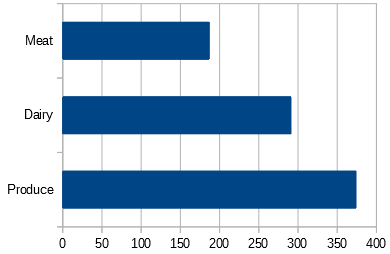
\includegraphics[width=\maxwidth{.95\linewidth}]{gfx/14-BarChart}
	\caption{Bar Chart}
	\label{14:fig01}
\end{figure}

With very large samples where observations are independent and random, the frequency distribution resembles a normal distribution, which looks like a bell-shaped curve when plotted. Figure \ref{14:fig02} shows the distribution of scores for the Scholastic Aptitude Test (\textit{SAT}) where most observations are clustered toward the center of the range with fewer observations toward the extremes. 

\begin{figure}[H]
	\centering
	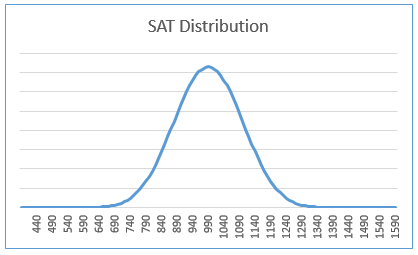
\includegraphics[width=\maxwidth{.95\linewidth}]{gfx/14-NormDist}
	\caption{Normal Distribution}
	\label{14:fig02}
\end{figure}

Central tendency is an estimate of the center of a distribution of values. There are three major estimates of central tendency: mean, median, and mode. The arithmetic mean (often simply called the ``mean'') is the simple average of all values in a given distribution. Consider a set of eight test scores: $ 15 $, $ 22 $, $ 21 $, $ 18 $, $ 36 $, $ 15 $, $ 25 $, $ 15 $. The arithmetic mean of these values is ($ 15 + 20 + 21 + 20 + 36 + 15 + 25 + 15)/8 = 20.875 $.

The median, is the middle value in a distribution. This is computed by ordering all values and selecting the one in the middle. In case there are two middle values (if there is an even number of values in a distribution), the median is the average of the two middle values. In the example test scores from the previous paragraph, the sorted values are: $ 15 , 15 , 15 , 18 , 22 , 21, 25, 36 $. The two middle values are $ 18 $ and $ 22 $ so the median is $ (18 + 22)/2 = 20 $. 

The mode is the most frequently occurring value in a distribution of values. Mode is normally only used for categorical data rather than numeric. For example, if an item on a survey asked whether respondents rented, leased, or owned their office building it would not make sense to try to find an ``average'' for those values, instead the most common response would be reported as the mode. 

Dispersion refers to the way values are spread around the central tendency, for example, how tightly or how widely are the values clustered around the mean. Two common measures of dispersion are the range and standard deviation. 

The range is the difference between the highest and lowest values in a distribution. The range in the test scores above is $ 36 - 15 = 21 $. The range is particularly sensitive to the presence of outliers, which makes its use problematic. For instance, if the highest value in the above distribution was $ 85 $ and the other vales remained the same, the range would be $ 85 - 15 = 70 $. 

Standard deviation corrects for outliers by calculating each value's distance from the mean. While that is a relatively complex calculation, all statistics software is able to easily find the standard deviation. In a normal distribution, 68\% of the observations lie within one standard deviation of the mean, 95\% within two standard deviations, and 99.7\% within three standard deviations.

\subsubsection{Bivariate Analysis}

Bivariate analysis examines how two variables are related to each other. The most common bivariate statistic is the correlation, which is a number between $ -1.00 $ and $ +1.00 $ denoting the strength of the relationship between two variables. For example, imagine a research project designed to relate age to the amount of money spent on groceries. If the amount of money spent increases as age increases then that would be a positive correlation but if the amount spent decreases as age increases then that would be a negative correlation. If the correlation is near zero then there is no relationship between age and the amount spent on groceries.

As an example, H{\"a}rdle\cite{hardlesmoothing} analyzed the duration and waiting time (in minutes) for eruptions of the Old Faithful Geyser in Yellowstone Park. There are $ 272 $ observations in that data set and Table \ref{14:tab02} shows the first five of those observations.

\begin{table}[H]
	\centering
	\begin{tabulary}{\linewidth}{CC}
		\hline
		Waiting & Eruption \\ 
		\hline
		$ 79 $ & $ 3.600 $ \\ 
		$ 54 $ & $ 1.800 $ \\ 
		$ 74 $ & $ 3.333 $ \\ 
		$ 62 $ & $ 2.283 $ \\ 
		$ 85 $ & $ 4.533 $ \\ 
		$ 55 $ & $ 2.883 $ \\ 
		\hline
	\end{tabulary} 
	\caption{Geyser Times}
	\label{14:tab02}
\end{table}

The correlation between these two variables is $ +0.901 $. Since the correlation is positive then as the waiting time goes up the duration also goes up. Figure \ref{14:fig06} graphs the eruption duration as a function of the waiting time and it is reasonably clear that as the waiting time increases (the right edge of the X-axis) the duration also tends to increase.

\begin{figure}[H]
	\centering
	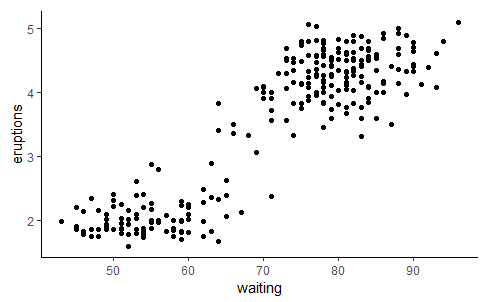
\includegraphics[width=\maxwidth{.95\linewidth}]{gfx/14_Faithful}
	\caption{Geyser Eruptions}
	\label{14:fig06}
\end{figure}

After computing a correlation, researchers are often interested in knowing whether the correlation is significant, that is to say, is there a true relationship between the variables or was the calculated correlation nothing more than mere chance. Answering such a question requires creating and testing a hypothesis. Suppose, then, the geyser researcher wrote this hypothesis, ``as the waiting time increases the duration of the eruption increases.'' This hypothesis also suggests another hypothesis, ``there is no relationship between the waiting time and duration of an eruption.'' While it seems like these are two hypotheses, they are actually a single hypothesis along with its opposite. The ``no relationship'' hypothesis is formally called the ``null hypothesis'' and that represents the status if there is no relationship. The null hypothesis is very important in research and all hypotheses that are researched also include an implied null hypothesis. For example, if a researcher states a hypothesis that in a grocery store moving the bread to the front of the store will increase bread sales then the null hypothesis is that moving the bread has no effect on sales. As a second example, if a researcher states a hypothesis that automobile tires perform better when warm than cold then the null hypothesis would be that temperature has no effect on tire performance.

For the geyser research project, the researcher would use a statistical procedure known as a two-tailed t-test to see if the eruption times are significant. The probability that a statistical result is caused by pure chance is called the \textit{p-value}. The p-value is compared with a desired significance level, which is the maximum level of risk the researcher will accept that the statistic is nothing more than pure chance. For most statistical analysis, the p-value is specified as $ 0.05 $. So, a p-value less than $ 0.05 $ indicates that the statistical evidence makes it reasonable to reject the null hypothesis and accept the researcher's original hypothesis. On the other hand, if the p-value is greater than $ 0.05 $, then the null hypothesis cannot be rejected. For the geyser data, the calculated p-value is less than $ 2.2 X 10^{-16} $ and since that is much smaller than $ 0.05 $ the researcher would conclude that the correlation between the eruption time and waiting time is significant.

Most research studies involve more than two variables. If there are multiple variables researchers need to use more powerful tools for analysis. One such tool is a correlational matrix. This is a graphic representation of the correlations between a number of variables. As an example, certain data were extracted from the 1974 \textit{Motor Trend} magazine for several automobiles and those data were used to create the correlation matrix found in Figure \ref{14:fig07}.

\begin{figure}[H]
	\centering
	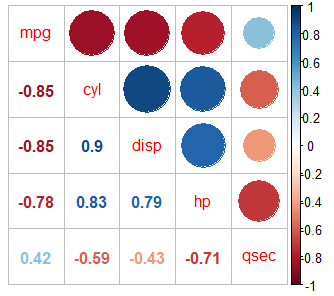
\includegraphics[width=\maxwidth{.95\linewidth}]{gfx/14_corplot}
	\caption{Correlation Matrix}
	\label{14:fig07}
\end{figure}

In Figure \ref{14:fig07}, the variable names are printed in the diagonal: ``mpg'' for ``Miles per Gallon,'' ``cyl'' for the number of cylinders in the engine, ``disp'' for the engine displacement, ``hp'' for the horsepower, and ``qsec'' for the time though a quarter mile course. The top triangle (with the colored circles) shows the strength and direction of the correlation. Blue circles represent positive correlation and red is negative. The size of the circle also indicates the strength of the correlation. With this type of display, researchers can very quickly find interesting correlations among even dozens of variables. The lower triangle (with the numbers) displays the correlation numerically, but color is also used so researchers can quickly find the strongest positive or negative correlations. As an example, the relationship between miles-per-gallon and the number of cylinders is $ -0.85 $.

Another common way of presenting multiple variables is with a cross-tabulation, often abbreviated to cross-tab. A cross-tab is a table that describes the frequency (or percentage) of all combinations of two or more nominal or categorical variables. 

As an example, the following cross-tab shows the survivors of the Titanic disaster by sex, age, and class of ticket.

\begin{table}[H]
	\centering
	\begin{tabulary}{\linewidth}{RRR}
		\hline
		\textbf{Class} & \textbf{Male} & \textbf{Female} \\ 
		\hline
		\multicolumn{3}{l}{\textit{Child}} \\
		1st  & $ 5 $  & $ 1 $ \\ 
		2nd  & $ 11 $ & $ 13 $ \\ 
		3rd  & $ 13 $ & $ 14 $ \\ 
		Crew & $ 0 $  & $ 0 $ \\ 
		\hline
		\multicolumn{3}{l}{\textit{Adult}} \\
		1st  & $ 57 $  & $ 140 $ \\ 
		2nd  & $ 14 $ & $ 80 $ \\ 
		3rd  & $ 75 $ & $ 76 $ \\ 
		Crew & $ 192 $  & $ 20 $ \\ 
		\hline
	\end{tabulary} 
	\caption{Titanic Survivors}
	\label{14:tab03}
\end{table}

\subsection{Quantitative Analysis: Inferential}
%TODO Bhattacherjee p 138
%TODO Start Here
Inferential statistics are the statistical procedures that are used to reach conclusions about associations between variables. They differ from descriptive statistics in that they are explicitly designed to test hypotheses. Numerous statistical procedures fall in this category, most of which are supported by modern statistical software such as SPSS and SAS. This chapter provides a short primer on only the most basic and frequent procedures; readers are advised to consult a formal text on statistics or take a course on statistics for more advanced procedures.

Basic Concepts

British philosopher Karl Popper said that theories can never be proven, only disproven. As an example, how can we prove that the sun will rise tomorrow? Popper said that just because the sun has risen every single day that we can remember does not necessarily mean that it will rise tomorrow, because inductively derived theories are only conjectures that may or may not be predictive of future phenomenon. Instead, he suggested that we may assume a theory that the sun will rise every day without necessarily proving it, and if the sun does not rise on a certain day, the theory is falsified and rejected. Likewise, we can only reject hypotheses based on contrary evidence but can never truly accept them because presence of evidence does not mean that we may not observe contrary evidence later. Because we cannot truly accept a hypothesis of interest (alternative hypothesis), we formulate a null hypothesis as the opposite of the alternative hypothesis, and then use empirical evidence to reject the null hypothesis to demonstrate indirect, probabilistic support for our alternative hypothesis. 

A second problem with testing hypothesized relationships in social science research is that the dependent variable may be influenced by an infinite number of extraneous variables and it is not plausible to measure and control for all of these extraneous effects. Hence, even if two variables may seem to be related in an observed sample, they may not be truly related in the population, and therefore inferential statistics are never certain or deterministic, but always probabilistic.

How do we know whether a relationship between two variables in an observed sample is significant, and not a matter of chance? Sir Ronald A. Fisher, one of the most prominent statisticians in history, established the basic guidelines for significance testing. He said that a statistical result may be considered significant if it can be shown that the probability of it being rejected due to chance is 5% or less. In inferential statistics, this probability is called the value, 5% is called the significance level (α), and the desired relationship between the p-value and α is denoted as: p≤0.05. The significance level is the maximum level of risk that we are willing to accept as the price of our inference from the sample to the population. If the p-value is less than 0.05 or 5%, it means that we have a 5% chance of being incorrect in rejecting the null hypothesis or having a Type I error. If p>0.05, we do not have enough evidence to reject the null hypothesis or accept the alternative hypothesis. 

We must also understand three related statistical concepts: sampling distribution, standard error, and confidence interval. A sampling distribution is the theoretical distribution of an infinite number of samples from the population of interest in your study. However, because a sample is never identical to the population, every sample always has some inherent level of error, called the standard error. If this standard error is small, then statistical estimates derived from the sample (such as sample mean) are reasonably good estimates of the population. The precision of our sample estimates is defined in terms of a confidence interval (CI). A 95% CI is defined as a range of plus or minus two standard deviations of the mean estimate, as derived from different samples in a sampling distribution. Hence, when we say that our observed sample estimate has a CI of 95%, what we mean is that we are confident that 95% of the time, the population parameter is within two standard deviations of our observed sample estimate. Jointly, the p-value and the CI give us a good idea of the probability of our result and how close it is from the corresponding population parameter.

General Linear Model

Most inferential statistical procedures in social science research are derived from a general family of statistical models called the general linear model (GLM). A model is an estimated mathematical equation that can be used to represent a set of data, and linear refers to a straight line. Hence, a GLM is a system of equations that can be used to represent linear patterns of relationships in observed data.

Figure 15.1. Two-variable linear model

The simplest type of GLM is a two-variable linear model that examines the relationship between one independent variable (the cause or predictor) and one dependent variable (the effect or outcome). Let us assume that these two variables are age and self-esteem respectively. The bivariate scatterplot for this relationship is shown in Figure 15.1, with age (predictor) along the horizontal or x-axis and self-esteem (outcome) along the vertical or y-axis. From the scatterplot, it appears that individual observations representing combinations of age and selfesteem generally seem to be scattered around an imaginary upward sloping straight line. We can estimate parameters of this line, such as its slope and intercept from the GLM. From highschool algebra, recall that straight lines can be represented using the mathematical equation y = mx + c, where m is the slope of the straight line (how much does y change for unit change in x) and c is the intercept term (what is the value of y when x is zero). In GLM, this equation is represented formally as:

$ y = \beta0 + \beta1 x + \epsilon $

where $ \beta0 $ is the slope, $ \beta1 $ is the intercept term, and $ \epsilon $ is the error term. $ \epsilon $ represents the deviation of actual observations from their estimated values, since most observations are close to the line but do not fall exactly on the line (i.e., the GLM is not perfect). Note that a linear model can have more than two predictors. To visualize a linear model with two predictors, imagine a three-dimensional cube, with the outcome (y) along the vertical axis, and the two predictors (say, x1 and x2) along the two horizontal axes along the base of the cube. A line that describes the relationship between two or more variables is called a regression line, $ \beta0 $ and $ \beta1 $ (and other beta values) are called regression coefficients, and the process of estimating regression coefficients is called regression analysis. The GLM for regression analysis with n predictor variables is:

$ y = \beta0 + \beta1 x1 + \beta2 x2 + \beta3 x3 + ... + \beta n xn + \epsilon $

In the above equation, predictor variables xi may represent independent variables or covariates (control variables). Covariates are variables that are not of theoretical interest but may have some impact on the dependent variable y and should be controlled, so that the residual effects of the independent variables of interest are detected more precisely. Covariates capture systematic errors in a regression equation while the error term ($ \epsilon $) captures random errors. Though most variables in the GLM tend to be interval or ratio-scaled, this does not have to be the case. Some predictor variables may even be nominal variables (e.g., gender: male or female), which are coded as dummy variables. These are variables that can assume one of only two possible values: 0 or 1 (in the gender example, ``male'' may be designated as 0 and ``female'' as 1 or vice versa). A set of n nominal variables is represented using n–1 dummy variables. For instance, industry sector, consisting of the agriculture, manufacturing, and service sectors, may be represented using a combination of two dummy variables (x1, x2), with (0, 0) for agriculture, (0, 1) for manufacturing, and (1, 1) for service. It does not matter which level of a nominal variable is coded as 0 and which level as 1, because 0 and 1 values are treated as two distinct groups (such as treatment and control groups in an experimental design), rather than as numeric quantities, and the statistical parameters of each group are estimated separately. 

The GLM is a very powerful statistical tool because it is not one single statistical method, but rather a family of methods that can be used to conduct sophisticated analysis with different types and quantities of predictor and outcome variables. If we have a dummy predictor variable, and we are comparing the effects of the two levels (0 and 1) of this dummy variable on the outcome variable, we are doing an analysis of variance (ANOVA). If we are doing ANOVA while controlling for the effects of one or more covariate, we have an analysis of covariance (ANCOVA). We can also have multiple outcome variables (e.g., y1, y1, … yn), which are represented using a “system of equations” consisting of a different equation for each outcome variable (each with its own unique set of regression coefficients). If multiple outcome variables are modeled as being predicted by the same set of predictor variables, the resulting analysis is called multivariate regression. If we are doing ANOVA or ANCOVA analysis with multiple outcome variables, the resulting analysis is a multivariate ANOVA (MANOVA) or multivariate ANCOVA (MANCOVA) respectively. If we model the outcome in one regression equation as a predictor in another equation in an interrelated system of regression equations, then we have a very sophisticated type of analysis called structural equation modeling. The most important problem in GLM is model specification, i.e., how to specify a regression equation (or a system of equations) to best represent the phenomenon of interest. Model specification should be based on theoretical considerations about the phenomenon being studied, rather than what fits the observed data best. The role of data is in validating the model, and not in its specification.

Two-Group Comparison

One of the simplest inferential analyses is comparing the post-test outcomes of treatment and control group subjects in a randomized post-test only control group design, such as whether students enrolled to a special program in mathematics perform better than those in a traditional math curriculum. In this case, the predictor variable is a dummy variable (1=treatment group, 0=control group), and the outcome variable, performance, is ratio scaled (e.g., score of a math test following the special program). The analytic technique for this simple design is a one-way ANOVA (one-way because it involves only one predictor variable), and the statistical test used is called a Student’s t-test (or t-test, in short). 

The t-test was introduced in 1908 by William Sealy Gosset, a chemist working for the Guiness Brewery in Dublin, Ireland to monitor the quality of stout – a dark beer popular with 19th century porters in London. Because his employer did not want to reveal the fact that it was using statistics for quality control, Gosset published the test in Biometrika using his pen name “Student” (he was a student of Sir Ronald Fisher), and the test involved calculating the value of t, which was a letter used frequently by Fisher to denote the difference between two groups. Hence, the name Student’s t-test, although Student’s identity was known to fellow statisticians. The t-test examines whether the means of two groups are statistically different from each other (non-directional or two-tailed test), or whether one group has a statistically larger (or smaller) mean than the other (directional or one-tailed test). In our example, if we wish to examine whether students in the special math curriculum perform better than those in traditional curriculum, we have a one-tailed test. This hypothesis can be stated as:

H0: $ \mu1 \leq \mu2 $ (null hypothesis)

H1: $ \mu1 > \mu2 $ (alternative hypothesis)

where $ \mu1 $ represents the mean population performance of students exposed to the special curriculum (treatment group) and $ \mu2 $ is the mean population performance of students with traditional curriculum (control group). Note that the null hypothesis is always the one with the “equal” sign, and the goal of all statistical significance tests is to reject the null hypothesis. How can we infer about the difference in population means using data from samples drawn from each population? From the hypothetical frequency distributions of the treatment and control group scores in Figure 15.2, the control group appears to have a bell-shaped (normal) distribution with a mean score of 45 (on a 0-100 scale), while the treatment group appear to have a mean score of 65. These means look different, but they are really sample means ( ), which may differ from their corresponding population means ($ \mu $) due to sampling error. Sample means are probabilistic estimates of population means within a certain confidence interval (95\% CI is sample mean + two standard errors, where standard error is the standard deviation of the distribution in sample means as taken from infinite samples of the population. Hence, statistical significance of population means depends not only on sample mean scores, but also on the standard error or the degree of spread in the frequency distribution of the sample means. If the spread is large (i.e., the two bell-shaped curves have a lot of overlap), then the 95\% CI of the two means may also be overlapping, and we cannot conclude with high probability (p<0.05) that that their corresponding population means are significantly different. However, if the curves have narrower spreads (i.e., they are less overlapping), then the CI of each mean may not overlap, and we reject the null hypothesis and say that the population means of the two groups are significantly different at p<0.05.

Figure 15.2. Student’s t-test

To conduct the t-test, we must first compute a t-statistic of the difference is sample means between the two groups. This statistic is the ratio of the difference in sample means relative to the difference in their variability of scores (standard error): where the numerator is the difference in sample means between the treatment group (Group 1) and the control group (Group 2) and the denominator is the standard error of the difference between the two groups, which in turn, can be estimated as: s2 is the variance and n is the sample size of each group. The t-statistic will be positive if the treatment mean is greater than the control mean. To examine if this t-statistic is large enough than that possible by chance, we must look up the probability or p-value associated with our computed t-statistic in statistical tables available in standard statistics text books or on the Internet or as computed by statistical software programs such as SAS and SPSS. This value is a function of the t-statistic, whether the t-test is one-tailed or two-tailed, and the degrees of freedom (df) or the number of values that can vary freely in the calculation of the statistic (usually a function of the sample size and the type of test being performed). The degree of freedom of the t-statistic is computed as: which often approximates to (n1+n2–2). If this p-value is smaller than a desired significance level (say $ \alpha = 0.05 $) or the highest level of risk (probability) we are willing to take to conclude that there is a treatment effect when in fact there is none (Type I error), then we can reject the null hypotheses.

After demonstrating whether the treatment group has a significantly higher mean than the control group, the next question usually is what is the effect size (ES) or the magnitude of the treatment effect relative to the control group? We can estimate the ES by conducting regression analysis with performance scores as the outcome variable (y) and a dummy coded treatment variable as the predictor variable (x) in a two-variable GLM. The regression coefficient of the treatment variable ($ \beta1 $), which is also the slope of the regression line ($ \beta1 = \Delta y/\Delta x $), is an estimate of the effect size. In the above example, since x is a dummy variable with two values (0 and 1), $ \Delta x = 1–0 = 1 $, and hence the effect size or $ \beta1 $ is simply the difference between treatment and control means ($ \Delta y = y1- y2 $).

Factorial Designs

Extending from the previous example, let us say that the effect of the special curriculum (treatment) relative to traditional curriculum (control) depends on the amount of instructional time (3 or 6 hours/week). Now, we have a 2 x 2 factorial design, with the two factors being curriculum type (special versus traditional) and instructional type (3 or 6 hours/week). Such a design not only helps us estimate the independent effect of each factor, called main effects, but also the joint effect of both factors, called the interaction effect. The generalized linear model for this two-way factorial design is designated as follows:

$ y = \beta0 + \beta1 x1 + \beta2 x2 + \beta3 x1 x2 + \epsilon $

where y represents students' post-treatment performance scores, x1 is the treatment (special versus traditional curriculum), x2 is instructional time (3 or 6 hours/week). Note that both x1 and x2 are dummy variables, and although x2 looks like a ratio-scale variable (3 or 6), it actually represents two categories in the factorial design. Regression coefficients $ \beta1 $ and $ \beta2 $ provide effect size estimates for the main effects and $ \beta3 $ for the interaction effect. Alternatively, the same factorial model can be analyzed using a two-way ANOVA analysis. Regression analysis involving multiple predictor variables is sometimes called multiple regression, which is different from multivariate regression that uses multiple outcome variables. 

A note on interpreting interaction effects. If $ \beta3 $ is significant, it implies that the effect of the treatment (curriculum type) on student performance depends on instructional time. In this case, we cannot meaningfully interpret the independent effect of the treatment ($ \beta1 $) or of instructional time ($ \beta2 $), because the two effects cannot be isolated from each other. Main effects are interpretable only when the interaction effect is non-significant. Covariates can be included in factorial designs as new variables, with new regression coefficients (e.g., $ \beta4 $). Covariates can be measured using interval or ratio scaled measures, even when the predictors of interest are designated as dummy variables. Interpretation of covariates also follows the same rules as that of any other predictor variable.

Other Quantitative Analysis

There are many other useful inferential statistical techniques, based on variations in the GLM, that are briefly mentioned here. Interested readers are referred to advanced text books or statistics courses for more information on these techniques:

Factor analysis is a data reduction technique that is used to statistically aggregate a large number of observed measures (items) into a smaller set of unobserved (latent) variables called factors based on their underlying bivariate correlation patterns. This technique is widely used for assessment of convergent and discriminant validity in multi-item measurement scales in social science research.

Discriminant analysis is a classificatory technique that aims to place a given observation in one of several nominal categories based on a linear combination of predictor variables. The technique is similar to multiple regression, except that the dependent variable is nominal. It is popular in marketing applications, such as for classifying customers or products into categories based on salient attributes as identified from large-scale surveys.

Logistic regression (or logit model) is a GLM in which the outcome variable is binary (0 or 1) and is presumed to follow a logistic distribution, and the goal of the regression analysis is to predict the probability of the successful outcome by fitting data into a logistic curve. An example is predicting the probability of heart attack within a specific period, based on predictors such as age, body mass index, exercise regimen, and so forth. Logistic regression is extremely popular in the medical sciences. Effect size estimation is based on an “odds ratio,” representing the odds of an event occurring in one group versus the other.

Probit regression (or probit model) is a GLM in which the outcome variable can vary between 0 and 1 (or can assume discrete values 0 and 1) and is presumed to follow a standard normal distribution, and the goal of the regression is to predict the probability of each outcome. This is a popular technique for predictive analysis in the actuarial science, financial services, insurance, and other industries for applications such as credit scoring based on a person’s credit rating, salary, debt and other information from her loan application. Probit and logit regression tend to demonstrate similar regression coefficients in comparable applications (binary outcomes); however the logit model is easier to compute and interpret.

Path analysis is a multivariate GLM technique for analyzing directional relationships among a set of variables. It allows for examination of complex nomological models where the dependent variable in one equation is the independent variable in another equation, and is widely used in contemporary social science research. 

Time series analysis is a technique for analyzing time series data, or variables that continually changes with time. Examples of applications include forecasting stock market fluctuations and urban crime rates. This technique is popular in econometrics, mathematical finance, and signal processing. Special techniques are used to correct for auto-correlation, or correlation within values of the same variable across time 


\section{Qualitative Analysis}

%TODO Bhattacherjee p 122
Qualitative analysis is the analysis of qualitative data such as text data from interview transcripts. Unlike quantitative analysis, which is statistics driven and largely independent of the researcher, qualitative analysis is heavily dependent on the researcher’s analytic and integrative skills and personal knowledge of the social context where the data is collected. The emphasis in qualitative analysis is “sense making” or understanding a phenomenon, rather than predicting or explaining. A creative and investigative mindset is needed for qualitative analysis, based on an ethically enlightened and participant-in-context attitude, and a set of analytic strategies. This chapter provides a brief overview of some of these qualitative analysis strategies. Interested readers are referred to more authoritative and detailed references such as Miles and Huberman’s (1984)17 seminal book on this topic. 

Grounded Theory

How can you analyze a vast set qualitative data acquired through participant observation, in-depth interviews, focus groups, narratives of audio/video recordings, or secondary documents? One of these techniques for analyzing text data is grounded theory – an inductive technique of interpreting recorded data about a social phenomenon to build theories about that phenomenon. The technique was developed by Glaser and Strauss (1967)18 in their method of constant comparative analysis of grounded theory research, and further refined by Strauss and Corbin (1990)19 to further illustrate specific coding techniques – a process of classifying and categorizing text data segments into a set of codes (concepts), categories (constructs), and relationships. The interpretations are “grounded in” (or based on) observed empirical data, hence the name. To ensure that the theory is based solely on observed evidence, the grounded theory approach requires that researchers suspend any preexisting theoretical expectations or biases before data analysis, and let the data dictate the formulation of the theory.

Strauss and Corbin (1998) describe three coding techniques for analyzing text data: open, axial, and selective. Open coding is a process aimed at identifying concepts or key ideas 

17 Miles M. B., Huberman A. M. (1984). Qualitative Data Analysis: A Sourcebook of New Methods. Newbury Park, CA: Sage Publications. 18 Glaser, B. and Strauss, A. (1967). The Discovery of Grounded Theory: Strategies for Qualitative Research, Chicago: Aldine. 19 Strauss, A. and Corbin, J. (1990). Basics of Qualitative Research: Grounded Theory Procedures and Techniques, Beverly Hills, CA: Sage Publications.

that are hidden within textual data, which are potentially related to the phenomenon of interest. The researcher examines the raw textual data line by line to identify discrete events, incidents, ideas, actions, perceptions, and interactions of relevance that are coded as concepts (hence called in vivo codes). Each concept is linked to specific portions of the text (coding unit) for later validation. Some concepts may be simple, clear, and unambiguous while others may be complex, ambiguous, and viewed differently by different participants. The coding unit may vary with the concepts being extracted. Simple concepts such as “organizational size” may include just a few words of text, while complex ones such as “organizational mission” may span several pages. Concepts can be named using the researcher’s own naming convention or standardized labels taken from the research literature. Once a basic set of concepts are identified, these concepts can then be used to code the remainder of the data, while simultaneously looking for new concepts and refining old concepts. While coding, it is important to identify the recognizable characteristics of each concept, such as its size, color, or level (e.g., high or low), so that similar concepts can be grouped together later. This coding technique is called “open” because the researcher is open to and actively seeking new concepts relevant to the phenomenon of interest.

Next, similar concepts are grouped into higher order categories. While concepts may be context-specific, categories tend to be broad and generalizable, and ultimately evolve into constructs in a grounded theory. Categories are needed to reduce the amount of concepts the researcher must work with and to build a “big picture” of the issues salient to understanding a social phenomenon. Categorization can be done is phases, by combining concepts into subcategories, and then subcategories into higher order categories. Constructs from the existing literature can be used to name these categories, particularly if the goal of the research is to extend current theories. However, caution must be taken while using existing constructs, as such constructs may bring with them commonly held beliefs and biases. For each category, its characteristics (or properties) and dimensions of each characteristic should be identified. The dimension represents a value of a characteristic along a continuum. For example, a “communication media” category may have a characteristic called “speed”, which can be dimensionalized as fast, medium, or slow. Such categorization helps differentiate between different kinds of communication media and enables researchers identify patterns in the data, such as which communication media is used for which types of tasks. The second phase of grounded theory is axial coding, where the categories and subcategories are assembled into causal relationships or hypotheses that can tentatively explain the phenomenon of interest. Although distinct from open coding, axial coding can be performed simultaneously with open coding. The relationships between categories may be clearly evident in the data or may be more subtle and implicit. In the latter instance, researchers may use a coding scheme (often called a “coding paradigm”, but different from the paradigms discussed in Chapter 3) to understand which categories represent conditions (the circumstances in which the phenomenon is embedded), actions/interactions (the responses of individuals to events under these conditions), and consequences (the outcomes of actions/ interactions). As conditions, actions/interactions, and consequences are identified, theoretical propositions start to emerge, and researchers can start explaining why a phenomenon occurs, under what conditions, and with what consequences.

The third and final phase of grounded theory is selective coding, which involves identifying a central category or a core variable and systematically and logically relating this central category to other categories. The central category can evolve from existing categories or can be a higher order category that subsumes previously coded categories. New data is selectively sampled to validate the central category and its relationships to other categories (i.e., the tentative theory). Selective coding limits the range of analysis, and makes it move fast. 

At the same time, the coder must watch out for other categories that may emerge from the new data that may be related to the phenomenon of interest (open coding), which may lead to further refinement of the initial theory. Hence, open, axial, and selective coding may proceed simultaneously. Coding of new data and theory refinement continues until theoretical saturation is reached, i.e., when additional data does not yield any marginal change in the core categories or the relationships.

The “constant comparison” process implies continuous rearrangement, aggregation, and refinement of categories, relationships, and interpretations based on increasing depth of understanding, and an iterative interplay of four stages of activities: (1) comparing incidents/texts assigned to each category (to validate the category), (2) integrating categories and their properties, (3) delimiting the theory (focusing on the core concepts and ignoring less relevant concepts), and (4) writing theory (using techniques like memoing, storylining, and diagramming that are discussed in the next chapter). Having a central category does not necessarily mean that all other categories can be integrated nicely around it. In order to identify key categories that are conditions, action/interactions, and consequences of the core category, Strauss and Corbin (1990) recommend several integration techniques, such as storylining, memoing, or concept mapping. In storylining, categories and relationships are used to explicate and/or refine a story of the observed phenomenon. Memos are theorized write-ups of ideas about substantive concepts and their theoretically coded relationships as they evolve during ground theory analysis, and are important tools to keep track of and refine ideas that develop during the analysis. Memoing is the process of using these memos to discover patterns and relationships between categories using two-by-two tables, diagrams, or figures, or other illustrative displays. Concept mapping is a graphical representation of concepts and relationships between those concepts (e.g., using boxes and arrows). The major concepts are typically laid out on one or more sheets of paper, blackboards, or using graphical software programs, linked to each other using arrows, and readjusted to best fit the observed data.

After a grounded theory is generated, it must be refined for internal consistency and logic. Researchers must ensure that the central construct has the stated characteristics and dimensions, and if not, the data analysis may be repeated. Researcher must then ensure that the characteristics and dimensions of all categories show variation. For example, if behavior frequency is one such category, then the data must provide evidence of both frequent performers and infrequent performers of the focal behavior. Finally, the theory must be validated by comparing it with raw data. If the theory contradicts with observed evidence, the coding process may be repeated to reconcile such contradictions or unexplained variations. 

\subsection{Quantitative vs. Qualitative}

Given their differences, it may come as no surprise that quantitative and qualitative research in psychology and related fields do not coexist in complete harmony. Some quantitative researchers criticize qualitative methods on the grounds that they lack objectivity, are difficult to evaluate in terms of reliability and validity, and do not allow generalization to people or situations other than those actually studied. At the same time, some qualitative researchers criticize quantitative methods on the grounds that they overlook the richness of human behavior and experience and instead answer simple questions about easily quantifiable variables.

In general, however, qualitative researchers are well aware of the issues of objectivity, reliability, validity, and generalizability. In fact, they have developed a number of frameworks for addressing these issues (which are beyond the scope of our discussion). And in general, quantitative researchers are well aware of the issue of oversimplification. They do not believe that all human behavior and experience can be adequately described in terms of a small number of variables and the statistical relationships among them. Instead, they use simplification as a strategy for uncovering general principles of human behavior.


\section{Combining Quantitative and Qualitative}

%TODO This comes from Terrell - Mixed Methods...
Quantitative research (i.e., a positivist paradigm) has historically been the
cornerstone of social-science research. Purists call for researchers to
“eliminate their biases, remain emotionally detached and uninvolved with the
objects of study and test or empirically justify their stated hypotheses”
(Johnson \& Onwuegbuzie, 2004, p.14).

Qualitative purists support a constructivist or interpretivist paradigm and
“contend that multiple-constructed realities abound, that time- and contextfree
generalizations are neither desirable nor possible, that research is valuebound,
that it is impossible to differentiate fully causes and effects, that logic
flows from specific to general and that knower and known cannot be
separated because the subjective knower is the only source of reality”
(Johnson \& Onwuegbuzie, 2004, p. 14).

The End of the “Paradigm Wars” and the Emergence of Mixed Methods
Calls in the 80's and 90's for ``a truce'' between the two major paradigms.

Many major authors and researchers felt that quantitative and qualitative research methodologies are compatible.

Paradigm relativism – ``the use of whatever philosophical and/or methodological approach (that) works for the particular research problem under study'' (Tashakkori \& Teddlie, 2008, p. 9).

Many social-scientists now believe there is no major problem area that should be studied exclusively with one research method.

Quantitative tells us ``if'' while qualitative tells us ``how or why.''

The Type of Multi-Method Approach Depends Upon Four Factors

Theoretical perspective
	Explicit – based firmly on a theory
	Implicit – based indirectly on a theory

Priority of strategy
	Equal
	Qualitative
	Quantitative

Sequence of data collection implementation
	Qualitative first
	Quantitative first
	No sequence

The point at which the data are integrated
	At data collection
	At data analysis
	At data interpretation
	With some combination

Sequential Explanatory

\begin{figure}[H]
	\centering
	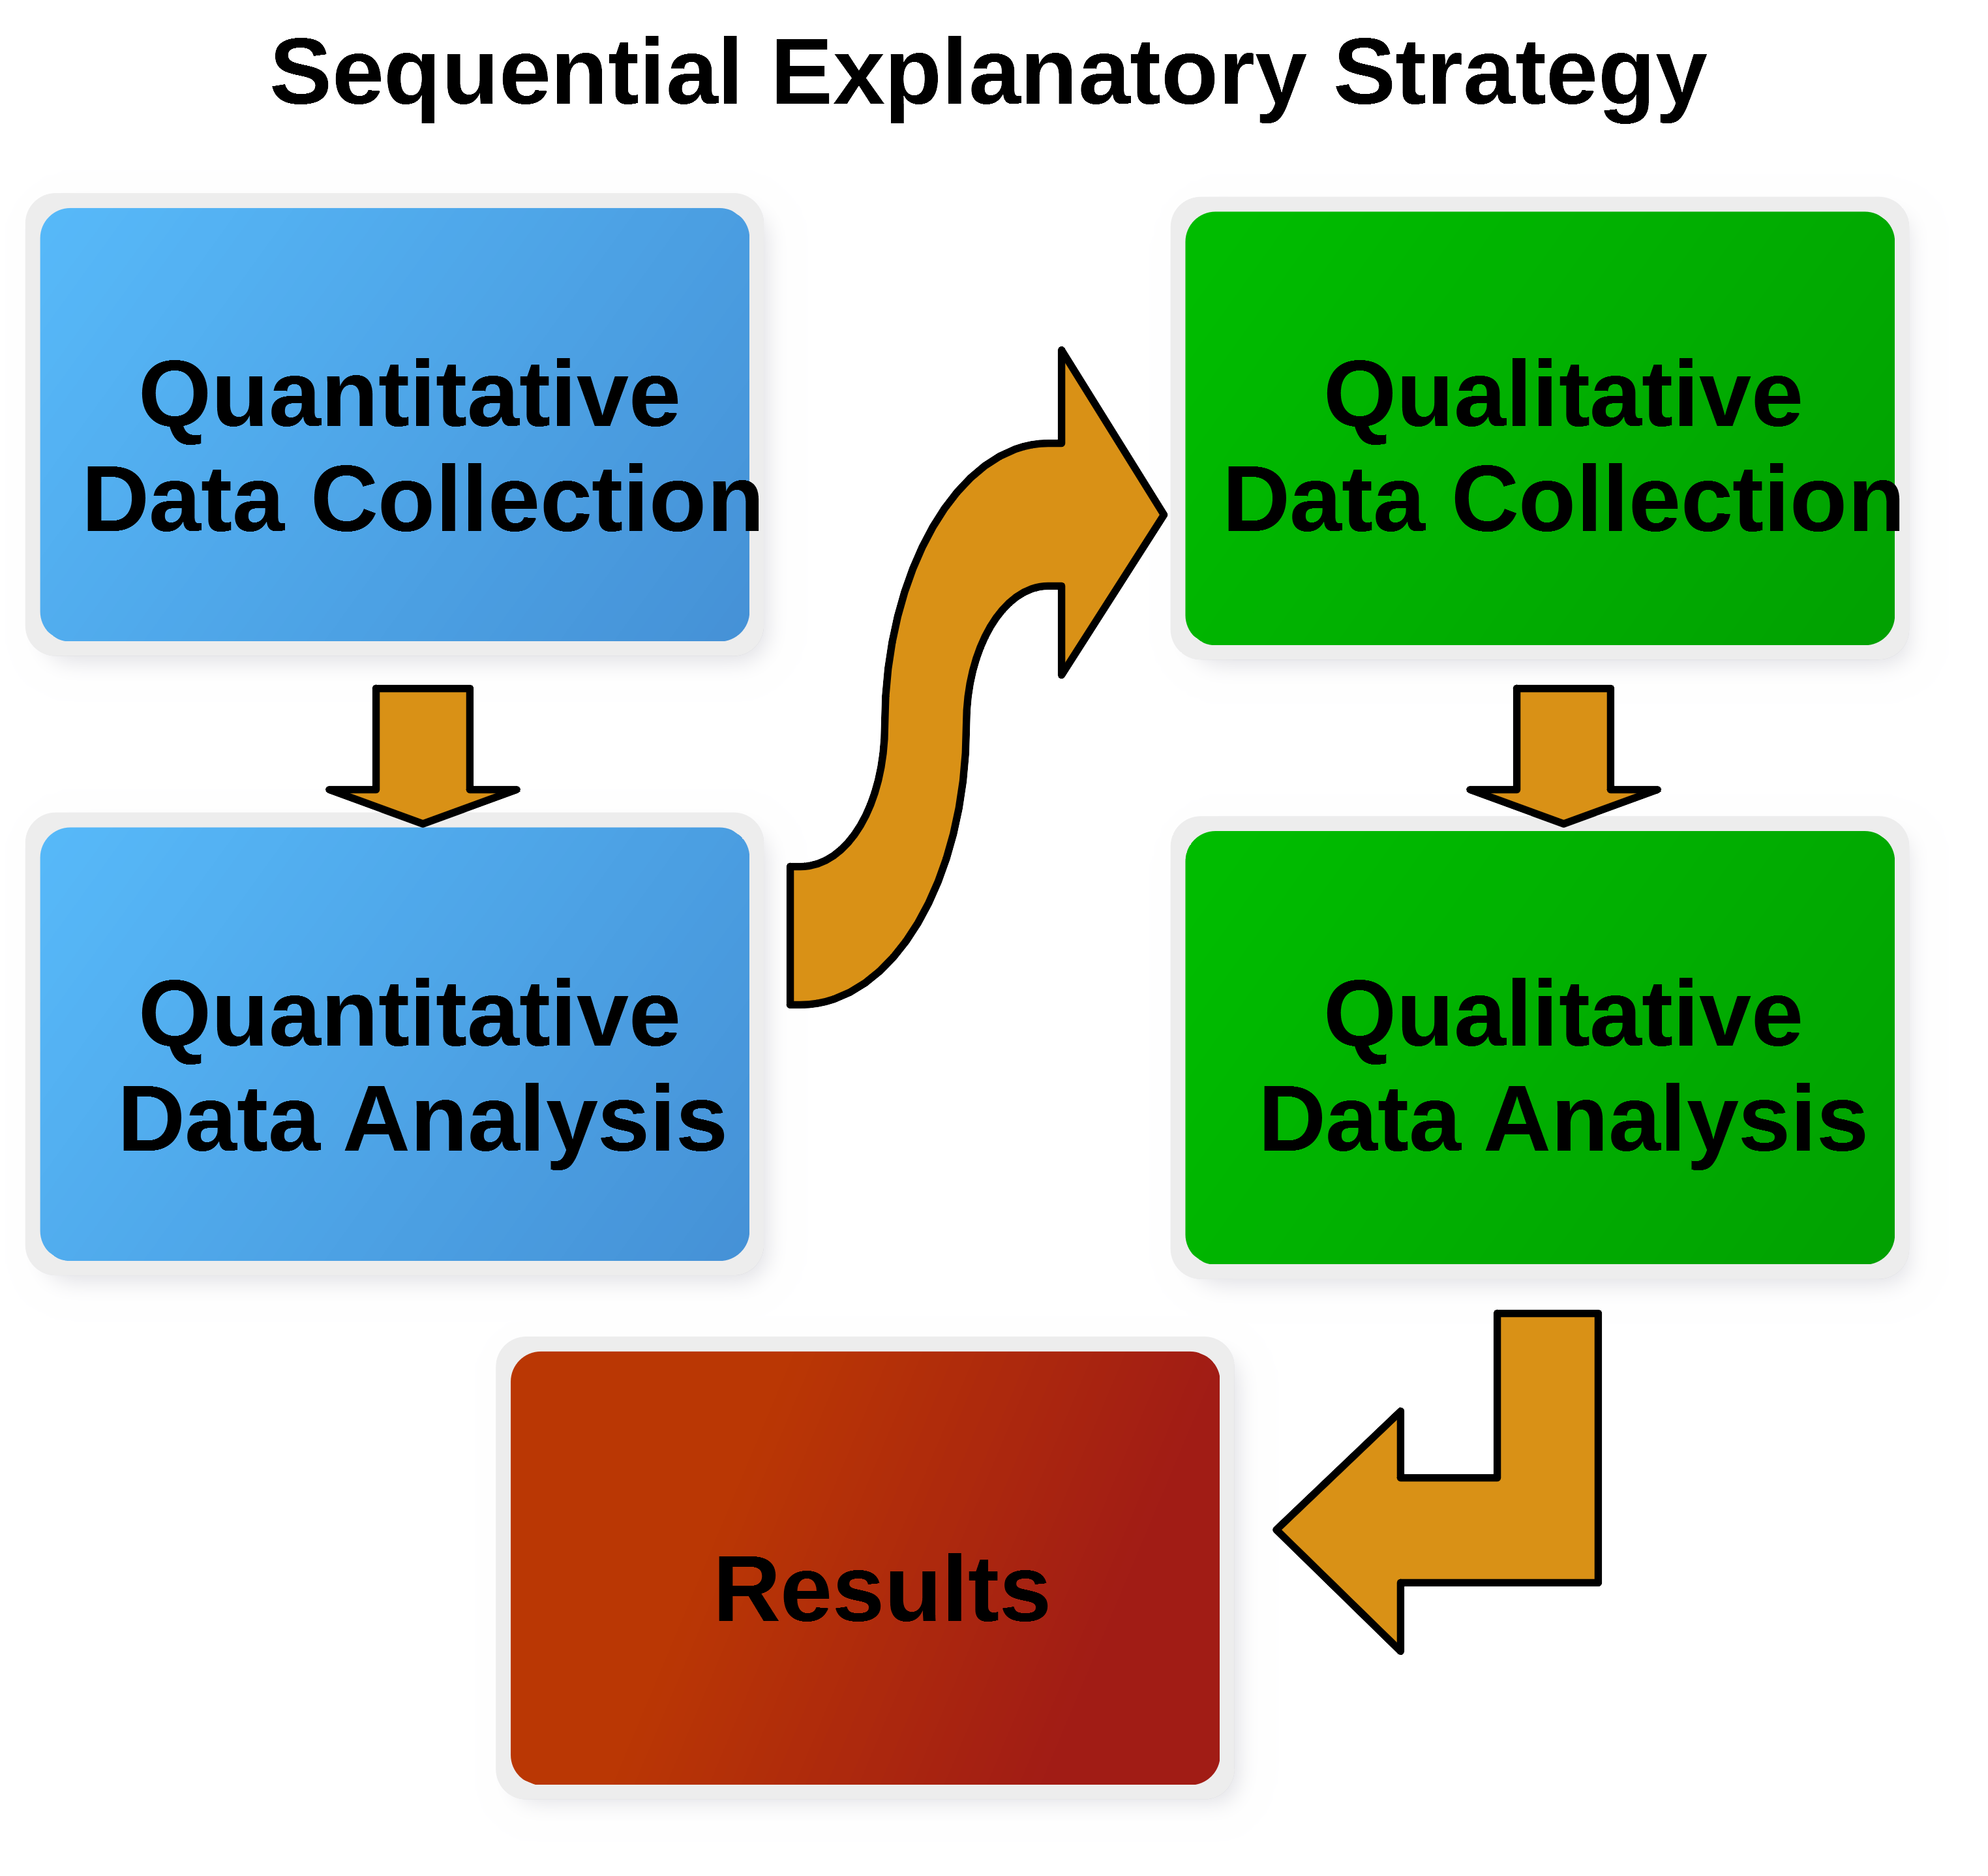
\includegraphics[width=\maxwidth{.95\linewidth}]{gfx/14-Seq_Explain}
	\caption{Sequential Explanatory}
	\label{14:fig90}
\end{figure}

Sequential Explanatory Strategy

The collection and analysis of quantitative data followed by the collection and analysis of qualitative data.

Equal priority is given to the two phases.

Data are integrated during interpretation.

Primary focus is to explain quantitative results by exploring certain results in more detail or helping explain unexpected results (e.g., using follow-up interviews to better understand the results of a quantitative study).

Strengths: relatively straight forward due to clear, distinct stages and easier to describe than concurrent strategies.

Weakness: very time consuming especially when both phases are given equal consideration
and priority.

Sequential Exploratory

\begin{figure}[H]
	\centering
	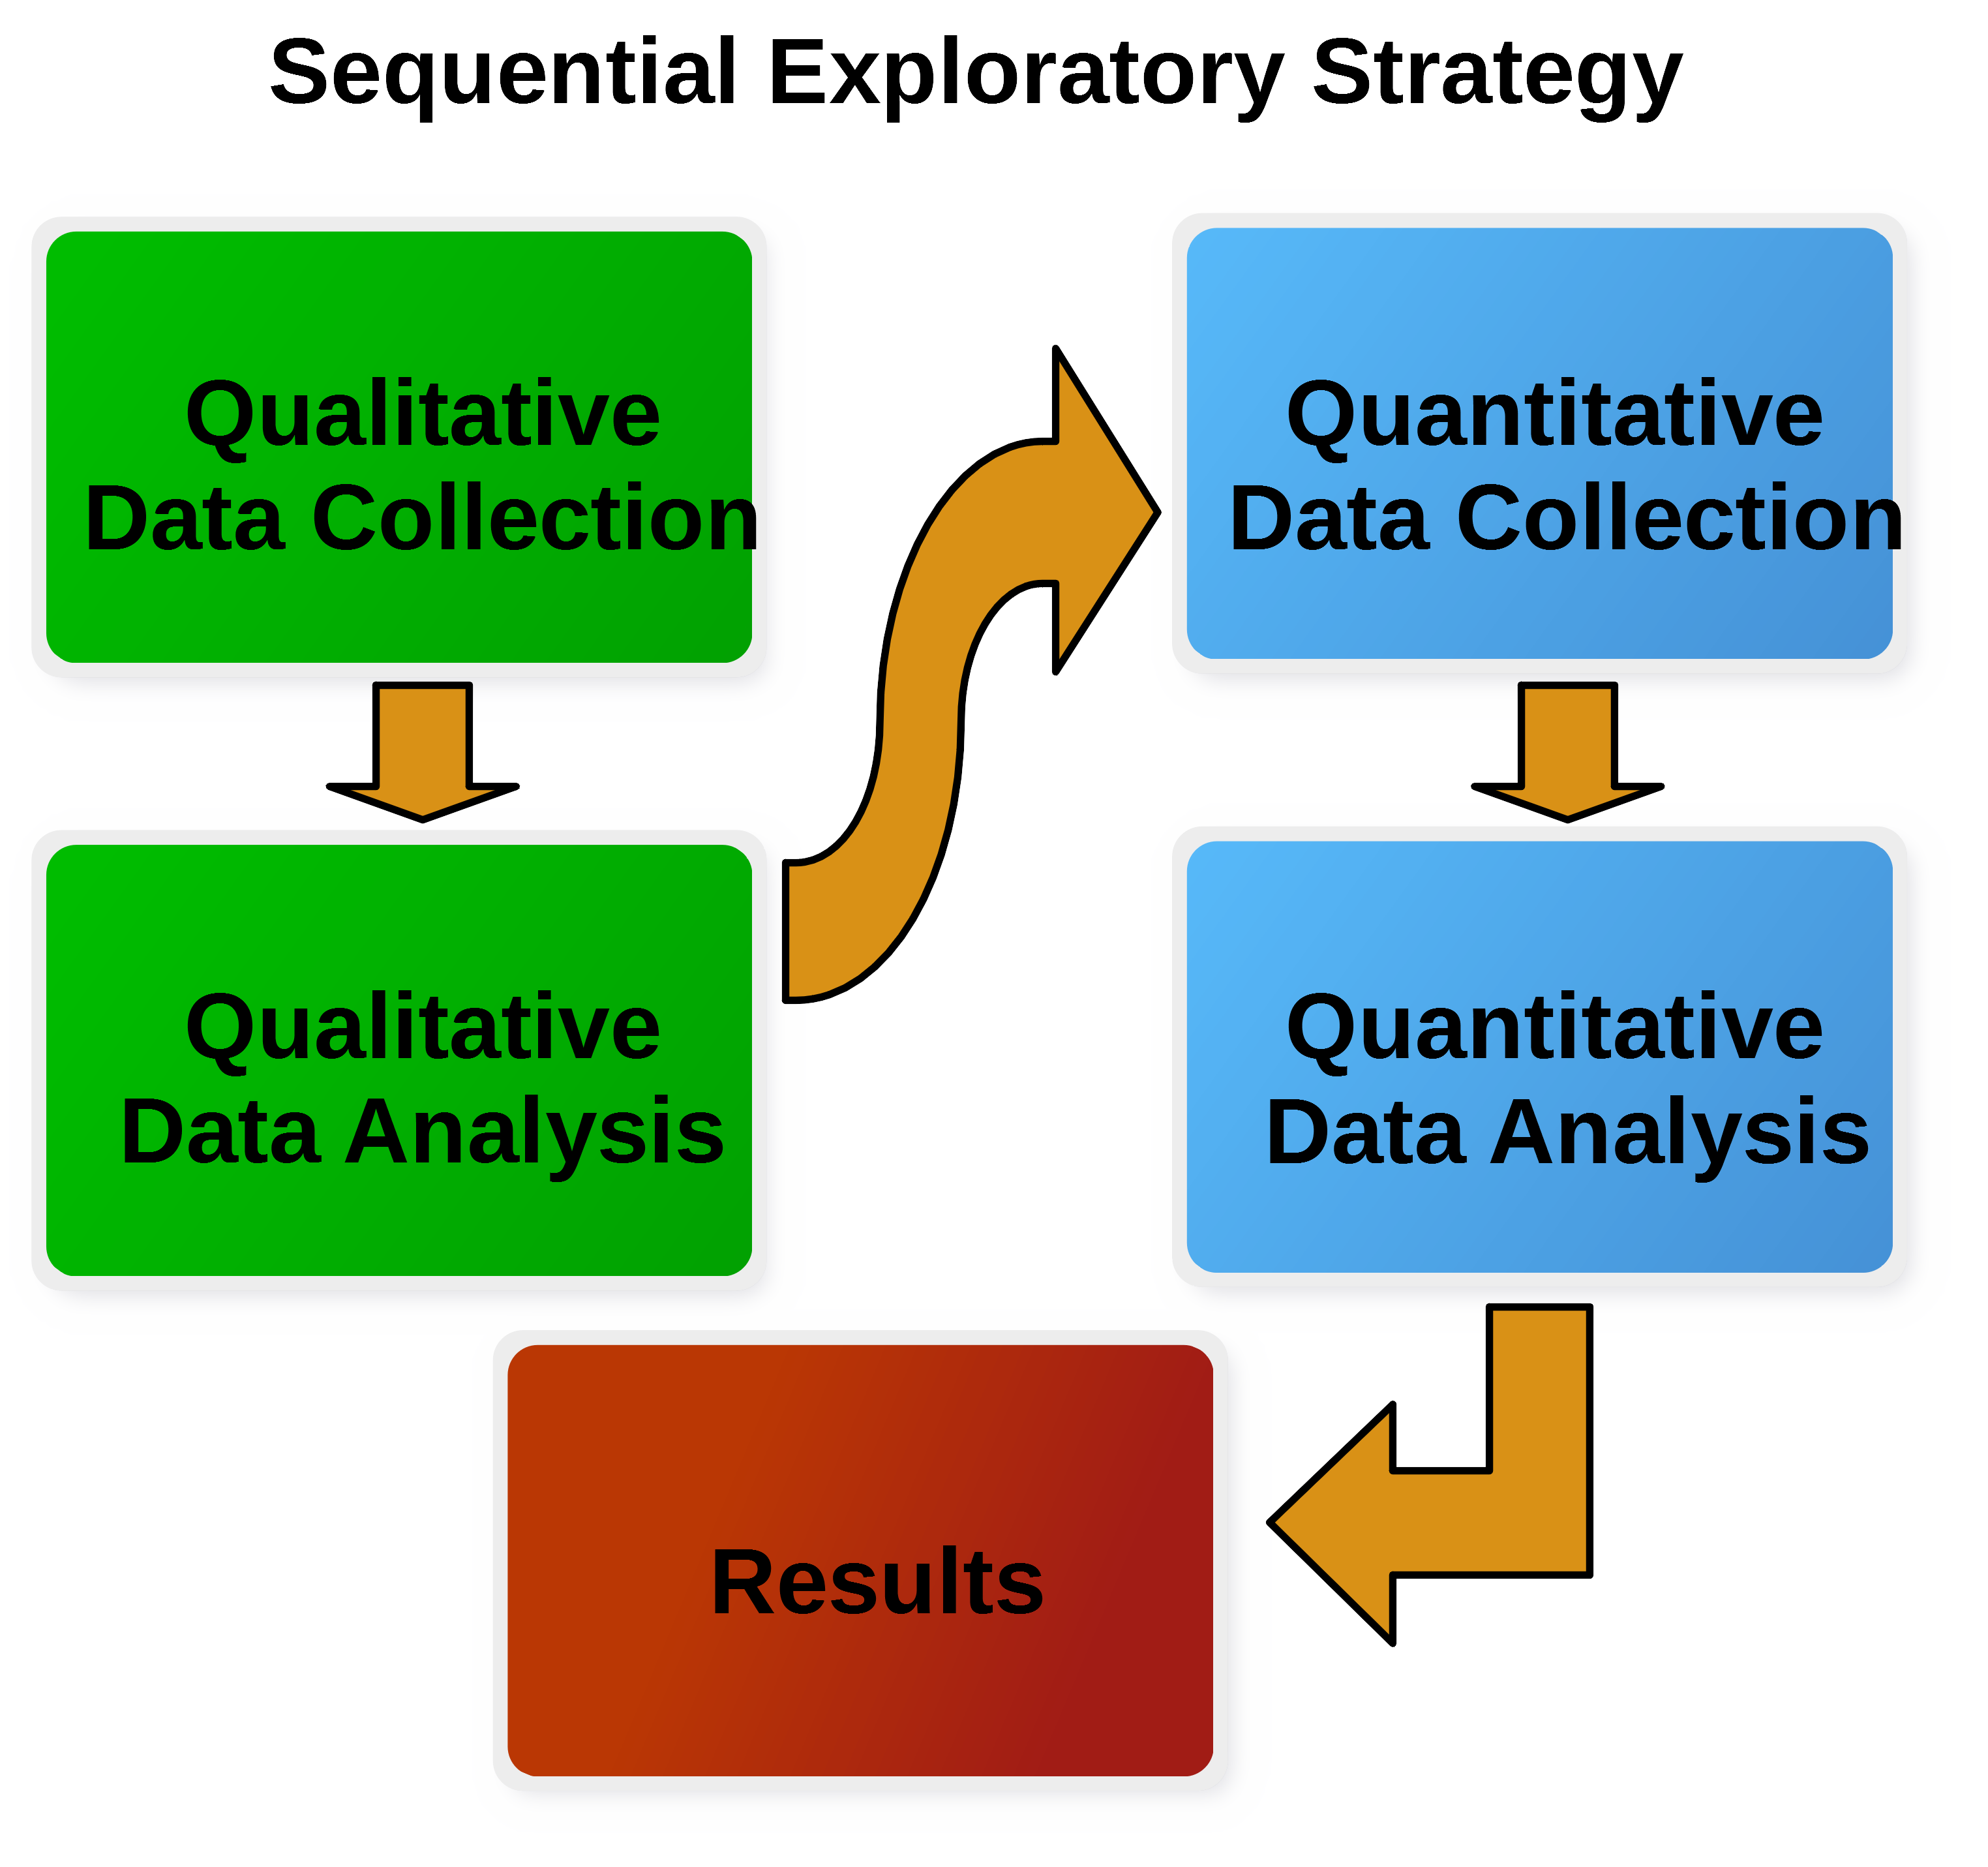
\includegraphics[width=\maxwidth{.95\linewidth}]{gfx/14-Seq_Explore}
	\caption{Sequential Exploratory}
	\label{14:fig91}
\end{figure}

Sequential Exploratory Strategy

The collection and analysis of qualitative data followed by the collection and analysis of
quantitative data.

Equal priority is given to the two phases but priority can be given to either.

Data are integrated during interpretation.

Used primarily to explore a phenomenon by:
	Testing elements of a theory
	Generalizing qualitative findings to different samples
	Development of instrumentation (e.g., using a small group to create instrumentation and then collecting quantitative data based on the instrumentation).

Strength: relatively straight forward due to clear, distinct stages and easier to describe than concurrent strategies.

Weakness: very time consuming especially when both phases are given equal consideration
and priority.

Triangulation

\begin{figure}[H]
	\centering
	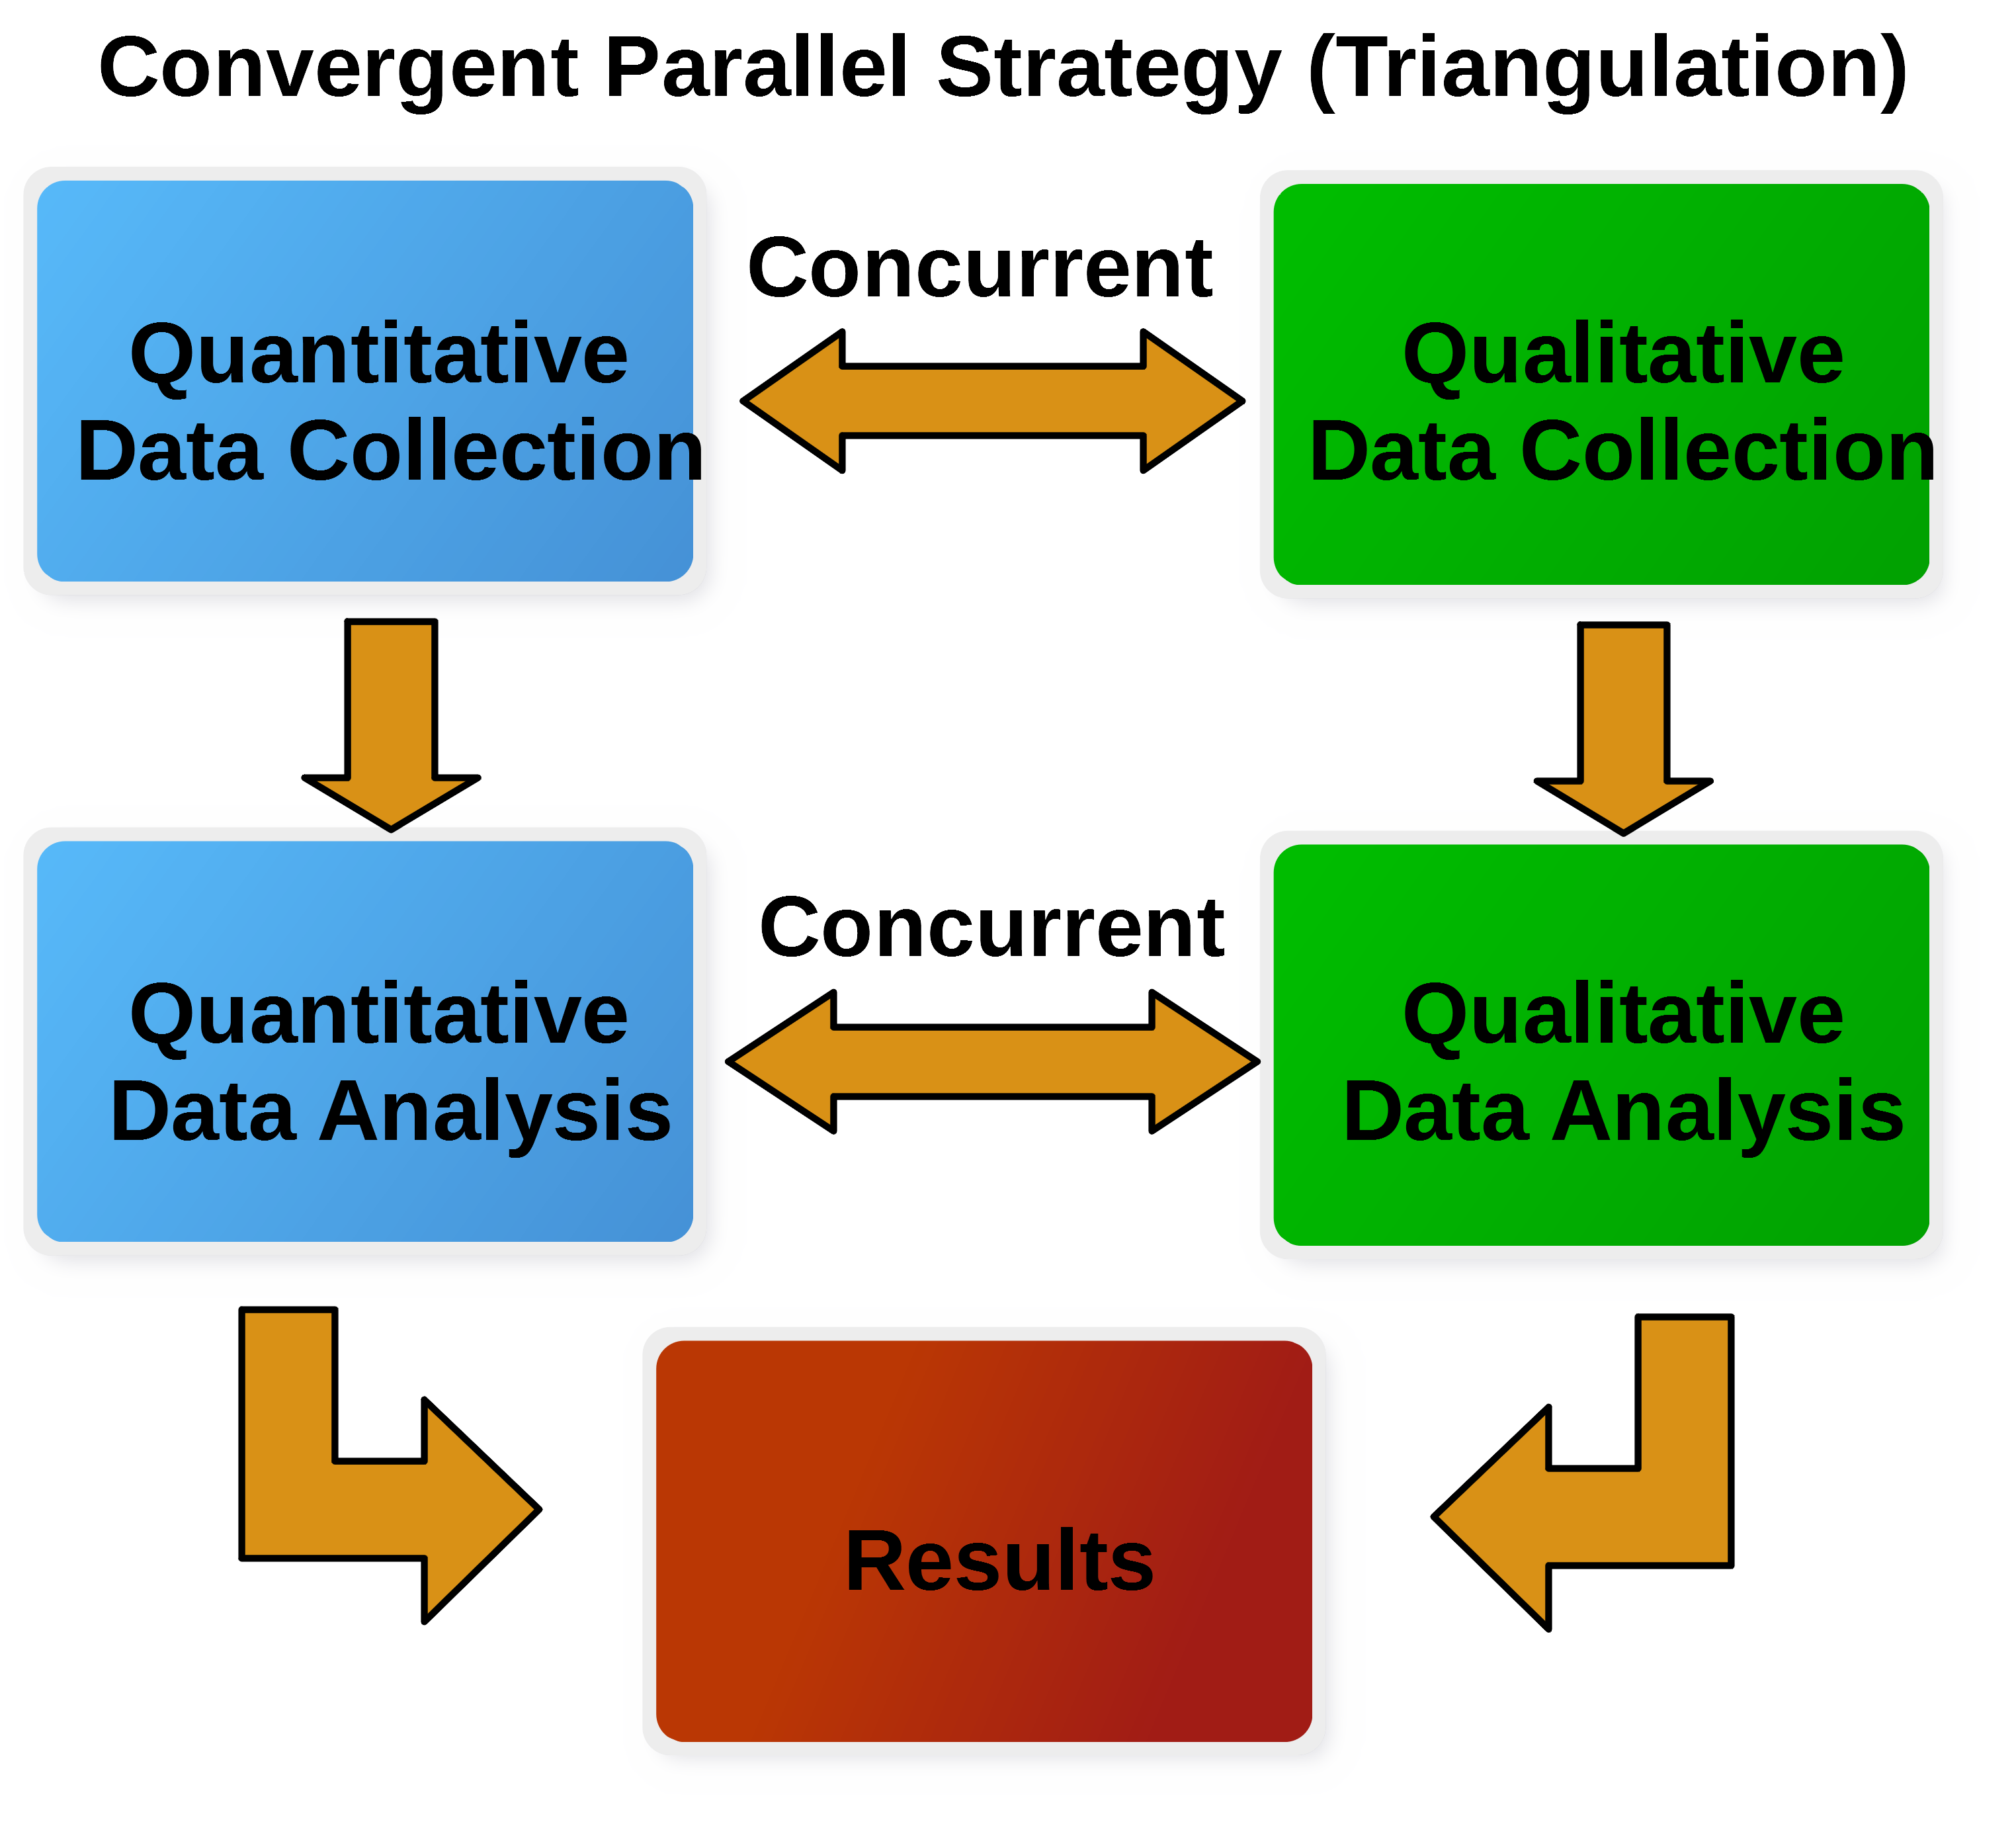
\includegraphics[width=\maxwidth{.95\linewidth}]{gfx/14-Triangulation}
	\caption{Triangulation}
	\label{14:fig92}
\end{figure}

Concurrent Triangulation Strategy

There are two concurrent data collection phases.

Priority should be equal but can be given to either approach.

Data are integrated during interpretation phase. The interpretation notes either a lack of convergence or convergence that strengthens knowledge claims. Data integration can also occur during analysis.

Primarily purpose for confirmation, corroboration or cross-validation within a single study.

Strengths: Familiar to many researchers. Shorter data collection time when compared to sequential methods. Offsets weaknesses inherent to one design by using both.

Weaknesses: Requires a great deal of expertise and effort to study the phenomenon under consideration using two different methods. It may be difficult to compare two types of data as well as resolve discrepancies if they arise.

%TODO from Lorenzini

Mixed-method research offers powerful tools to investigate complex systems and processes in health, education, and social science. These areas have been increasingly using complex mixed-method research designs1. This method encompasses the complete research procedure, including philosophical assumptions, research questions, design, collection, analysis, integration and structures of presentation of data and results2. \footnote{The material in this section is adapted from Lorenzini, \textit{Mixed-Method Research in the Health Sciences}\cite{lorenzini2017mixed}}

The nature of the research question guides the selection of the method. Researchers in healthcare field use a quantitative methodology to study and answer research questions on causality3, generalization, and magnitude of effect. The qualitative methodology is the choice of researchers who seek to answer research questions that explore how or why a given phenomenon occurs, to develop a theory or describe on the subjectivity of an individual experience1.

Mixed-method research is delineated considering the strengths of each of the two approaches, quantitative and qualitative, and, due to this, it is a methodological innovation increasingly used to address contemporary issues in health services. An indication of the increased interest of this method was the publication of the first best-practices guideline on mixed-methods research in the health sciences by the National Institutes of Health. The guideline was elaborated by researchers and research Project reviewers funded by the Office of Behavioral and Social Sciences at the National Institutes of Health4.

Over the course of the years, several definitions of mixed methods have emerged incorporating characteristics of method, philosophy, processes, and research projects. Currently, researchers are focused on defining the essential characteristics of mixed-methods research, which are described in literature as5:

a) In response to questions and hypotheses, collection and analysis of quantitative and qualitative data takes place;

b) Rigorous procedures are used to carry out quantitative and qualitative research;

c) There is integration or combination of results;

d) Procedures are developed in which data collection, analysis, and integration takes place: mixed-methods design;

e) It reports to the theory and philosophical principles related to those procedures.

It is, therefore, pointed out that this method involves the triangulation of quantitative and qualitative data in a single project. Those approaches complement each other inasmuch as they represent words and numbers, the two fundamental languages of human communication. Among the advantages of mixed methods, it may be stated that researchers can permit the manifestation of the best of each of the methods, avoiding the possible limitations of a single approach. This methodological orientation is indicated when a data source may be insufficient to answer the research problem or when the results need to be explained and the exploratory findings need generalization.

It is often argued that the quantitative approach is not able to capture the specificities in terms of what is understood of the context where the study  took place. Still, researchers in this line are at the vanguard and possible or eventual subjective interpretations are rarely discussed. Qualitative research compensates for these weaknesses. However, qualitative research is seen as deficient due to the personal interpretations made by the researcher, the bias created because of this, the small number of participatns, and the difficulty to generalize the results. Quantitative research, in turn, does not have those weaknesses. Thus, the combination of potentialities of one approach compensates for the weaknesses of the other. Thereby, the mixed-methods research provides more evidence for the study of a research problem than the use of one of the two approaches in an isolated manner. By using mixed methods, researchers can use all available tools, rather  than confinning themselves to data collection strategies commonly associated with quantitative or qualitative research. 

In current literature, ten advances in mixed-methods research are described, (along the last 5 years) to be incorporated by researchers in their projects:

a) Include information on the skills researchers/research teams have in qualitative, quantitative, and mixed-method research;

b) Create study aims for the qualitative, quantitative, and mixed-methods components;

c) Write a justification for the use of mixed methods;

d) Develop/present a mixed-methods design for the procedures chosen;

e) Portray this design with a diagram and/or implementation matrix;

f) Be specific about the point of integration in the design;

g) Create tables with results of the two phases together to show integration and write inferences;

h) Select a conceptual framework/theoretical model for the project and align it to the design;

i) Develop/present validity (research integrity) in the design/project;

j) Carry out multiple publications stemming from the mixed-methods project.

Regarding the theoretical perspective that guides the execution of the research project, it is important to highlight that all researchers are oriented by theories or guiding structures and postulate hypotheses in their research that may be explicit or implicit and, in this case, are not cited in texts5. To self-evaluate and check their own proficiency and skills in mixed-methods research, researchers can use the instrument6, developed and tested for such. Thus, it is possible to identify each researcher’s strong points and the areas that can still be developed and/or improved.

Researchers who master one of the approaches and who come from different epistemological perspectives, often find themselves working together forming a team to conduct mixedmethods research. To improve the dynamics of these teams, it is necessary for their members to develop the capacity to articulate their own research philosophy, visions, values, and objectives. Still, it is important to facilitate group interactions by creating conditions for values to be shared through dialogue, defining objectives, and developing trust. Systematically, it is quite important to optimize the values that promote and support dialectic pluralism and participation from stakeholders in research7.

A big challenge for researchers who commonly work with only one of the approaches is the integration of the data and the results. This stage raises the research method to a level that would not be reached by simply putting together the results of separate research, qualitative and quantitative, conducted without full attention to integration. This challenge is described, qualitatively, as the need to produce a whole through integration that is greater than the sum of the qualitative and quantitative parts individually. Quantitatively, authors express this idea as 1 + 1 = 3. That is, quantitative + qualitative = more than their individual components8-9.

Integration in mixed-methods research may occur in three distinct moments. In the study design, integration occurs through three basic projects - exploratory sequential, explanatory sequential, and convergent - and through four advanced frameworks - multi-stage or multiphasic, intervention, case study, and participatory10.

Integration at method level occurs through four approaches: “connection” of data, where a database is linked to another through sampling; “construction”, where a database informs the data collection approach of another; “fusion”, where the data from both bases are joined for analysis; “incorporation”, where data collection and analysis may be linked in several points10.

Integration during the interpretation and presentation of results occurs through narration, data transformation and joint display, according  to the methodological design chosen for the project. When researchers integrate data through narration, they describe qualitative and quantitative findings in one or more articles. There is three approaches to carry out integration in this way: a) write both qualitative and quantitative data together based on a theme or concept; b) present both types of data in a single publication, but in separate sessions; c) publish the findings  in separate articles, as may occur - for example - in multiphasic or multi-stage projects, where an intervention can be carried out via Randomized Clinical Trial (RCT) and interviews. In this example, the authors published an article with the findings from the interviews11, and only briefly mentioned the RCT12, which has been previously published10.

Integration through data transformation takes place in two phases. In the first phase, a type of data must be converted into another type of data (qualitative data to quantitative or quantitative data to qualitative). For example, qualitative data can be transformed through numerical counting and variables using content analysis. In the second phase, the data transformed is then integrated with the data that has not been transformed10. Integration of results presented through joint displays9, including the theory that guided the research since its conception facilitates visualization and provides insights on the analytical process of interpretation, enabling a unique form of representation or communication that is better captured visually than by isolated words. The addition of theoretical lenses to show  the integration in the joint displays is a notable characteristic, considered as an advance in mixed methods9.

Adjustment of the integration permits coherently observing and describing the quantitative and qualitative results, confirming them, and expanding their comprehension. Disagreement may occur if the qualitative and quantitative data are inconsistent, incongruent, contradict each other, and demonstrate conflict or discrepancies between each other.

The application of integration principles and practices may help researchers to leverage the strong points of mixed methods10. Recommendations are found in literature about the best practices9:

a) Identify the quantitative and qualitative results;

b) Be consistent with the design used in the method;

c) Be consistent with the integration methodology;

d) Identify inferences, meta-inferences, and insights generated.

Mixed methods offer a new framework to think about health services research with the potential to generate meta-inferences and unique insights on phenomena expressed in a multifaceted manner, related to access, quality, and the safe provision of healthcare13. When research questions can be best answered through this method, researchers need to dedicate themselves and make careful choices to conduct the integration process. Proper attention to integration in the stages of study conception and design, method, interpretation, and presentation of results can improve the quality of mixed-methods research in the health area and generate rigorous and important evidence to improve health care, services, systems, and healthcare policies.



\section{Summary}\label{ch14:summary}

Lorem ipsum dolor sit amet, consectetuer adipiscing elit. Aenean commodo ligula eget dolor. Aenean massa. Cum sociis natoque penatibus et


\ctparttext{After a research project is completed, the investigator must report the results of the project, often in both written and oral forms. This chapter concerns the reporting process. }
\part{Reporting}
\cleardoublepage
%*****************************************
\chapter{Presenting Research}
%*****************************************
% Blackstone p 159
% Need to check Bhat and Saylor on this
%TODO Status: Pre-draft

\section{Introduction}

\footnote{Most of the material in this chapter was adopted from McLean, \textit{Business Communication for Success}\cite{mclean2012business}}Most researchers hope that their work will have relevance to others besides themselves. As such, research is in some ways a public activity. While the work may be conducted by an individual in a private setting, the knowledge gained from that work should be shared with  peers and other parties who may have an interest. Understanding how to share research is an important aspect of the research process.

\section{What and With Whom to Share}

When preparing to share work with others, researchers must decide what to share, with whom to share it, and in what format(s) to share it. This section considers the ``what'' and ``with whom'' aspects while later sections cover the various formats and mechanisms through which research is shared.

\subsubsection{Sharing It All}

Because conducting research is a scholarly pursuit and because researchers generally aim to reach a true understanding of business and economics processes, it is crucial that all aspects of research, the good, the bad, and the ugly, are shared. Doing so helps ensure that others will understand, be able to build from, and effectively critique the work.

It is important to share all aspects of a research project for ethical reasons and to permit other researchers to replicate the work. The following questions will aid researchers in preparing to share research with others.

\begin{enumerate}
	\item Why was the research conducted?
	\item How was the research conducted?
	\item For whom was the research conducted?
	\item What conclusions can be reasonably drawn from this research?
	\item How could the research have been improved?
\end{enumerate}

Answering these questions help researchers be honest with themselves and the readers about their own personal interest, investments, or biases with respect to the work. The third question helps identify the major stakeholders, like funders, research participants, or others who share something in common with the research project (e.g., members of the community or social group who were involved in the research). These groups may be interested in the outcome of the research but may also be a source of bias. The last two questions help identify the strengths and weaknesses of the research project and could point the way for future projects.

\subsubsection{Knowing Your Audience}

An important decision for researchers is determining with whom to share the results. Certainly, the most obvious candidates with are other researchers working in the same field. Other potential audiences include stakeholders, reporters and other media representatives, policymakers, and members of the public more generally.

While the findings of a research project would never be altered for different audiences, understanding the audience helps frame the research report in a way that is most meaningful to that group. For example, the report for a project about the spending habits of elderly pensioners may be much different if rendered for a group of business owners, a governmental committee on aging, the funding agency, and a community meeting. In all cases, researchers would share the study's major findings, but the method of presentation and level of detail would vary by audience.

It would be expected that the greatest amount of detail, including data collection method, sampling, and analytic strategy, would be shared with colleagues and the funding agency. In addition, the funding agency may want information about the exact time line for the project along with any bureaucratic hiccups encountered. With a community meeting, though, a more succinct summary of the important findings using less technical jargon would be appropriate.

\section{Oral Presentations}

Researchers frequently make presentations to their peers in settings like conferences or departmental meetings. These presentations are excellent means for feedback and help researchers prepare to write up and publish their work. Presentations might be formal talks, either as part of a panel at a professional conference or to some other group of peers or other interested parties; less formal roundtable discussions, another common professional conference format; or posters that are displayed in some specially designated area.

When preparing a formal talk, it is very important for researchers to get details well in advance about the time limit for the presentation, requirements for questions from the audience, and whether visual aids, such PowerPoint slides, are expected. At conferences, the typical formal talk is usually expected to last between 15 and 20 minutes. Once researchers start talking about something as as important as their own research, it is common for them to become so engrossed that they forget to watch the clock and finds themselves running short of time. To avoid this all-too-common occurrence, it is crucial that presenters practice in advance, and time themselves.

One common mistake made in formal presentations of research work is in setting up the problem the research addresses. Audience members are usually more interested to hear about the researcher's work work than to hear the results of a long list of previous related studies. While written reports must discuss related previous studies, presentations must use the precious time available to highlight the current research project. Another mistake is to simply read the research paper verbatim. Nothing will bore an audience more quickly than hearing a presenter drone on while reading aloud. Finally, a presentation should highlight only the key points of the study, which, generally, include the research question, methodological approach, major findings, and a few final takeaways.

In less formal round table presentations, the aim is usually to help stimulate a conversation about a topic. Normally, several research projects are presented so the time available for each is normally shorter than in a formal presentation. Also, round table presentations always includes time for a conversation following the presentations. Round tables are especially useful when a research project is in the early stages of development. For example, perhaps a researcher has conducted a pilot study and is interested in ideas about where to take the study next. A round table is also an excellent place for a preview of potential objections reviewers may raise with respect to the project's approach or conclusions. Finally, round tables are great places to network and meet other scholars who share common interests.

Finally, a poster presentation is a visual representation a research project. Often, poster sessions are tables lined up in a conference area where researchers have a visual display on the table but also stand by to answer questions. A poster should not be just pages from the report pasted onto a poster board, rather, researchers decide how to tell the ``story'' of the work in graphs, charts, tables, and other images. Bulleted points are acceptable as long as the people walking by can quickly read and grasp the major argument and findings. Posters, like round tables, can be quite helpful at the early stages of a research project because they are designed to encourage the audience to engage in conversation about the research. It is not necessary to share every detail of a research project in a poster, the point is to share highlights and then discuss the details with people who are interested.

Most books about oral presentations divide presentations into several broad types.

\begin{description}
	\item[Speech to inform] Increase the audience's knowledge, teach about a topic
	or issue, and share the speaker's expertise.
	\item[Speech to demonstrate] Show the audience how to use, operate, or do
	something.
	\item[Speech to persuade] Influence the audience by presenting arguments
	intended to change attitudes, beliefs, or values.
	\item[Speech to entertain] Amuse the audience by engaging them in a
	relatively light-hearted speech that may have a serious point or goal.
	\item[Ceremonial speech] Perform a ritual function, such as give a toast at a
	wedding reception or a eulogy at a funeral.
\end{description}

Often, presentations are stressful since most people do not like speaking in public. However, the following tips may help.

\begin{itemize}
	\item Perfection is not required. Letting go of perfection can be the hardest guideline for speakers to apply to themselves. It is human nature to compare ourselves to others. It seems odd, but most people can forgive another researcher for the occasional slip or ``umm'' during a speech, but then turn right around and chastise themselves for making the same error. Everyone has both strengths and weaknesses and researchers must learn where they can improve is an important first step. The old saying is that Rome was not built in a day and good speakers are not developed overnight. It is true that no one wants to see a researcher fail during a presentation so audience members are generally very forgiving of minor speaking faults.
	\item Take the time to prepare and get organized. Researchers know the topic for the speech (normally a research report) and they are speaking in order to inform or persuade audience members to consider an idea. One of the best ways to build confidence is to know the material being presented ``inside out.''
	\item Public speaking is not unlike participating in a conversation. In regular conversations, researchers do not give a second thought to the process of saying something and then waiting for a reply. A public speech follows a similar pattern, but the reply is normally in the form of a non-verbal body language.
\end{itemize}

There are certain to be various obstacles arise in a presentation.

\begin{itemize}
	\item Language. Researchers work in fields where there are acronyms and insider jargon. As long as a presenter is 100\% certain that everyone in the audience understands some term then it is acceptable to use that term, but if there is any doubt then speakers should defer to common terms. As an example, soldiers may understand a sentence like ``I left the CHU in the COP and was heading to the DFAC when a fast mover dropped a JDAM in the village.'' People who lack military experience would not be able to understand that sentence.
	\item Culture. Everyone's culture is different and a speaker must understand that the audience's culture may be different enough that communication becomes challenging.
	\item Role. The speaker and audience may play very different roles in an organization and those roles may create barriers to communication. For example, researchers presenting to a room full of C-level executives would face a much different communications problem than if the room was filled with line workers. Effective speakers must understand the roles of the audience members and then speak in a way that is understandable to those people.
	\item Goal. Each of the audience members will have a goal in mind when attending the presentation. Occasionally, the goal may only be that they were assigned to attend the presentation; but more often than not, researchers will be presenting at a conference where the audience members select to attend the session. As much as possible, the speaker should attempt to understand the audience members' goals and then address those goals.
	\item Ethnocentrism. One obstacle to be avoided is for the researcher, or audience members, to exhibit a feeling that they are somehow superior to everyone else. While that can come from ethnicity, it is also a result of scholarly ``snobbish'' behavior, prejudice, or even stereotypes.
\end{itemize}

\subsection{Visual Aids}

Nearly all research presentations include some sort of visual aid. It is much easier for a speaker to use a graph or chart than to verbally describe some relationship in the data. When preparing visual aids, keep in mind that they should be...

\begin{itemize}
	\item Big. They need to be large enough to be seen from the back row of the auditorium. For graphs and charts this may be easy enough to arrange since those visuals can be made larger on the screen, but for a physical artifact it may be impossible to magnify it so its utility may be questioned.
	\item Clear. The visual needs to clearly convey whatever message is intended.
	\item Simple. There is an old rule of thumb about visual aids: 6 X 6, which means no more than six lines of text and six words per line.
	\item Consistent. All visuals should use a consistent style so audience members do not have to first learn how to read the graphic but can focus, instead, on the information being presented.
\end{itemize}

Color is a powerful communication tool, but speakers must be careful with color. First, keep in mind that some audience members will not be able to distinguish between two or more colors in the visual aid so never use color as the sole information source. Also, avoid using too many colors on one chart, a few well-placed colors are always more powerful than a lot of colors sprinkled seemingly at random around the visual. The following tips may help.

\begin{itemize}
	\item Keep visual aids simple.
	\item Use one key idea per slide.
	\item Avoid clutter, noise, and overwhelming slides.
	\item Use large, bold fonts that the audience can read from at least twenty 	feet from the screen.
	\item Use contrasting colors to create a dynamic effect.
	\item Use analogous colors to unify your presentation.
	\item Use clip art with permission and sparingly.
	\item Edit and proofread each slide with care and caution.
	\item Use copies of your visuals available as handouts after your presentation.
	\item Check the presentation room beforehand.
	\item Have a backup plan in case technology fails, such as providing printed visuals.
\end{itemize}

\section{Written Presentations}

Written reports that will be read by other scholars generally follow a formal format that is outlined by the publication journal. However, most scholarly reports include an abstract, an introduction, a literature review, a discussion of research methodology, a presentation of findings, and some concluding remarks and discussion about implications of the work. Reports written for scholarly consumption also contain a list of references and many include tables or charts that visually represent some component of the findings. Reading published research in business or economics is an excellent way to develop an understanding of the core components of scholarly research reports and to begin to learn how to write those components.

Reports written for public consumption differ from those written for scholarly consumption. As noted elsewhere in this chapter, knowing the audience is crucial when preparing a written report. Whoever your audience, it is important to keep in mind that scientific evidence is being reported. Writers must take seriously their roles as business researchers and be mindful of their place among peers in the discipline. Findings must be presented as clearly and honestly as possible; appropriate recognition must be afforded to the scholars who have come before, even if the research raises questions about their work; and readers should be engaged in a discussion about the research and potential avenues for further inquiry. Normally, research writers will never meet the readers face-to-face, but it is beneficial to imagine what the readers would ask and provide a detailed response in the written report.

Finally, it is extremely important to not to commit plagiarism in a research report. Presenting someone else's words or ideas as if they are the researcher's own is among the most egregious transgressions a scholar can commit. Indeed, plagiarism has ended many careers (Maffly, 2011) [4] and many students' opportunities to pursue degrees (Go, 2008). [5] 

\subsection{Writing Style}

Writing generally falls into one of three styles, colloquial, casual, and formal.

\subsubsection{Colloquial Style}

Colloquial language is an informal, conversational style of writing. It differs from standard business English in that it often makes use of colorful expressions, slang, and regional phrases. As a result, it can be difficult to understand for an English learner or a person from a different region of the country. Sometimes colloquialism takes the form of a word difference; for example, the difference between a ``Coke,'' a ``tonic,'' a ``pop,'' and a ``soda pop'' primarily depends on where you live. Colloquial phrases can also take the form of a saying. For example, in certain parts of the United States, the phrases ``dumb as a box of rocks'' and ``sharp as a tack'' both refer to a person's intelligence.

Colloquial writing may be permissible, and even preferable, in some business contexts. For example, a marketing letter describing a folksy product such as a wood stove or an old-fashioned popcorn popper might use a colloquial style to create a feeling of relaxing at home with loved ones. Still, it is important to consider how colloquial language  appears to the audience. Will the meaning of the chosen words be clear to a reader who is from a different part of the country? Will a folksy tone sound like the writer is ``talking down'' to the audience? A final point to remember is that colloquial style is not an excuse for using expressions that are sexist, racist, profane, or otherwise offensive.

\subsubsection{Casual Style}

Casual language involves everyday words and expressions in a familiar group context, such as conversations with family or close friends. The emphasis is on the communication interaction itself, and less about the hierarchy, power, control, or social rank of the individuals communicating. Casual communication is the written equivalent of wearing casual attire, like a t-shirt and jeans. When writing for business, a casual style is usually out of place; instead, a respectful, professional tone represents both the researcher and the company well.

\subsubsection{Formal Style}

Formal language is communication that focuses on professional expression with attention to roles, protocol, and appearance. It is characterized by professional vocabulary and syntax. That is, writers using a formal style tend to use a more sophisticated vocabulary, a greater variety of words, and more words with multiple syllables, not for the purpose of throwing big words around, but to enhance the formal mood of the document. They also tend to use more complex syntax, resulting in sentences that are longer and contain more subordinate clauses.

The appropriate style for a particular business document may be very formal, or less so. If a subordinate replies to an email from the supervisor, the exchange may be informal in that it is fluid and relaxed, without much forethought or fanfare, but it will still reflect the formality of the business environment. The subordinate will be careful to use an informative subject line, a semi-formal salutation (``Hi Mr. Smith'' is typical in e-mails), and a brief discussion about the topic at hand. Probably, the subordinate will also check grammar and spelling before clicking ``send.''

A formal document such as a proposal or an annual report will involve a great deal of planning and preparation, and its style may not be fluid or relaxed. Instead, it may use distinct language to emphasize the prestige and professionalism of the company. As an example, imagine a marketing letter that will be printed on company letterhead and mailed to a hundred sales prospects. Naturally, the letter should represent the company in a positive light and may include a sentence like ``The Widget 300 is our premium offering in the line; we have designed it for ease of movement and efficiency of use, with your success foremost in our mind.'' But in an e-mail or a tweet, an informal sentence may be used, ``W300 -- good stapler.''

\subsubsection{Plagiarism}

Writing in a business context means that writers represent both themselves and the company. While good writing can be part of both the writer's and the company's success, it can also expose the company to unintended consequences and legal responsibility. It is important to keep in mind that the words will keep on existing long after the writer has moved on to other projects. This can become an issue if the words exaggerate, state false claims, or defame a person or legal entity such as a competing company. Another important issue is plagiarism, which is using someone else's writing without giving credit to the source. Whether the ``cribbed'' material is taken from a printed book, a Web site, or a blog, plagiarism is a violation of copyright law and will also likely violate company policies. 

Closely related to plagiarism is libel, which is the written form of defamation, or a false statement that damages a reputation. If a false statement of fact that concerns and harms the person defamed is published, including publication in a digital or online environment, the author of that statement may be sued for libel. If the person defamed is a public figure they must prove malice or the intention to do harm, but if the victim is a private person, libel applies even if the offense cannot be proven to be malicious. Under the United States First Amendment writers have a right to express opinions, but the words used, and how they are used, are relevant to their interpretation as opinion versus fact. Writers must always be careful to qualify what they write and to do no harm.

\subsection{Report Format}

Research reports tend to follow a format that has evolved over many years.

\begin{description}
	\item[Title] This should be a concise description of the research findings.
	\item[Abstract] This is a very brief synopsis of the research findings. The exact size of the abstract is determined by the publisher, but they generally tend to be about 250 words in length.
	\item[Table of Contents] A TOC is not always used, especially for shorter reports. The publisher would determine if a TOC is important in the report.
	\item[Introduction]	This is a short description of the research project, why it was pursued and the anticipated result. The research thesis is often included in the introduction. Also, a few brief details of the methods and results is often found in the introduction.
	\item[Literature Review] This is normally one of the longer parts of the report. It surveys all of the related research in an effort to position the current research in the universe of prior research. Some literature reviews are structured chronologically while others are structured thematically. Regardless, there is a clear indication of where the current research project ``fits'' among prior research.
	\item[Methodology] This is a description of the method used during the research project. It would include information on how the sampling frame was selected, what sorts of data were gathered, and how those data were analyzed. This should be written thoroughly enough that another researcher could duplicate the project if desired.
	\item[Results] This details the results of the research project; however, the \textit{interpretation} of the results is normally saved for the ``discussion'' section of the report.
	\item[Discussion] This is a discussion about the relevance of the research project and how it fits with other research identified in the literature review. This would also describe any weaknesses of the research project and offer suggestions about how those could have been overcome.
	\item[Conclusion] This is a brief final summary of the entire research project, including the major findings. This would also suggest future research that would complement the current project.
	\item[Appendices] While appendices are not commonly used, when needed they are included at this point in the report.
	\item[Bibliography] All references used in the report are fully cited here so a reader could find all original research reports mentioned in the literature review if desired.
\end{description}

While there are almost as many formal research report formats as there are publishers or universities that process those reports, the above is a good general-purpose guideline of the types of sections often needed for publication.

\section{Disseminating Findings}

This section focuses on disseminating the written results of a research project. Dissemination refers to ``a planned process that involves consideration of target audiences and the settings in which research findings are to be received and, where appropriate, communicating and interacting with wider policy and…service audiences in ways that will facilitate research uptake in decision-making processes and practice'' (Wilson, Petticrew, Calnan, \& Natareth, 2010, p. 91). [1] In other words, dissemination of research findings involves careful planning, thought, consideration of target audiences, and communication with those audiences. Writing up results from a research project and having others take notice are two entirely different propositions. In fact, the general rule of thumb is that people will not take notice unless they are encouraged to do so. To paraphrase the classic line from the film \textit{Field of Dreams}, just because you build it does not mean they will come.

Disseminating research findings successfully requires determining who the audience is, where that audience is located, and how to reach them. When considering who the audience is, think about who is likely to take interest in the research project. The audience might include those who do not express enthusiastic interest but might nevertheless benefit from an awareness of the research. Of course, the research participants and those who share some characteristics in common with those participants are likely to have some interest in what was discovered in the course of the research. Other scholars who study similar topics are another obvious audience for the work. Perhaps there are policymakers who should take note of the work. Organizations that do work in an area related to the topic of the research project are another possibility. Finally, any and all inquisitive and engaged members of the public represent a possible audience for the work.

Where the audience is located should be fairly obvious once the composition of that audience is determined. The research participants are known since they were part of the study. Interested scholars can be found at professional conferences and via publications such as professional organizations' newsletters and scholarly journals. Policymakers include state and federal representatives who, at least in theory, should be available to hear a constituent speak on matters of policy interest. Organizations that do work in an area related to the research topic can be found with a simple web search. Finally, disseminating findings to the general public could take any number of forms: a letter to the editor of a local newspaper, a blog, or even a Facebook post.

Finally, determining how to reach the target audience will vary depending on which specific audience is of interest. The strategy should be determined by the norms of the audience. For example, scholarly journals provide author submission instructions that clearly define requirements for researchers wishing to disseminate their work via that journal. The same is true for newspaper editorials; check your newspaper's website for details about how to format and submit letters to the editor. To reach out to political representatives, a call to their offices or a simple web search should information about how to proceed.

Researchers who have conducted high-quality research and have findings that are likely to be of interest to any constituents besides themselves would have a duty as a scholar to share those findings. 

\section{Summary}\label{ch15:summary}

Lorem ipsum dolor sit amet, consectetuer adipiscing elit. Aenean commodo ligula eget dolor. Aenean massa. Cum sociis natoque penatibus et



%*********************************************************************
% Backmatter
%*********************************************************************
%\appendix
%\renewcommand{\thechapter}{\alph{chapter}}
\cleardoublepage
\part{Appendix}
%%********************************************************************
% Appendix
%*******************************************************
% If problems with the headers: get headings in appendix etc. right
%\markboth{\spacedlowsmallcaps{Appendix}}{\spacedlowsmallcaps{Appendix}}
\chapter{Appendix}

\section*{Glossary}

\begin{enumerate}
	
	\item \textbf{Boundary Conditions} (Chapter 2)
	
	\item \textbf{Constructivism} A philosophical stance that reality is a construct of the human mind and is, therefore, subjective. Normally, qualitative research methods are used by researchers who are constructivists. (Chapter 1)
	
	\item \textbf{Constructs} (Chapter 2)
	
	\item \textbf{Deductive Research} A research methodology that works from a general theory to specific observations. This is sometimes called the ``theory-testing'' form of research.
	
	\item \textbf{Epistomology} A branch of philosophy that is concerned with the sources of knowledge. (Chapter 1)
	
	\item \textbf{Falsifiability} To have credence, a hypothesis must be disapprovable; that is, there must be a way to prove it wrong.
	
	\item \textbf{Grounded Theory} (Chapter 2)
	
	\item \textbf{Idiographic} An explanation for an observed phenomenon that explains only a single case and is not applicable to a wider population. (Chapter 2)
	
	\item \textbf{Inductive Research} A research methodolody that works from specific observations to a general theory. This is sometimes called the ``theory-building'' form of research.
	
	\item \textbf{Logic} (Chapter 2)
	
	\item \textbf{Macro-Level Research} (Chapter 2)
	
	\item \textbf{Meso-Level Research} (Chapter 2)
	
	\item \textbf{Micro-Level Research} (Chapter 2)
	
	\item \textbf{Nomothetic} An explanation for an observed phenomenon that is applicable across a wide population rather than a single example. (Chapter 2)
	
	\item \textbf{Objectivism} A philosophical stance that there exists an objective reality can be studied and understood. (Chapter 1)
	
	\item \textbf{Ontology} The branch of philosophy that is concerned with the nature of reality. (Chapter 1)
	
	\item \textbf{Paradigm} A pattern or model of how things work in the world. (Chapter 1)
	
	\item \textbf{Parsimony} A fundamental aspect of research that states if two or more competing explanations are considered then the simplest must be accepted. Thus, researcher would state that the pyramids were built by humans using known technology rather than aliens in spaceships. (Chapter 1)
	
	\item \textbf{Positivism} (Chapter 2)
	
	\item \textbf{Postmodernism} (Chapter 2)
	
	\item \textbf{Precision} Research projects must precisely focus on one aspect of a problem or they will become so broad that their value will be diminished. (Chapter 1)
	
	\item \textbf{Propositions} (Chapter 2)
	
	\item \textbf{Replicability} A research project must be able to be replicated by other researchers or at other times in order to be considered sound. (Chapter 1)
	
\end{enumerate}


\cleardoublepage
\section*{Bibliography}

\subsection*{\ref{ch01:introduction}:  \nameref{ch01:introduction}}

\begin{description}

	\item Bobbitt-Zeher, Donna, and Douglas B. Downey. "Number of siblings and friendship nominations among adolescents." Journal of Family Issues 34.9 (2013): 1175-1193.
	
	\item Ellwood, David, and Thomas J. Kane. "Who is getting a college education? Family background and the growing gaps in enrollment." Securing the future: Investing in children from birth to college (2000): 283-324.

	\item Twain, Mark. Following the equator. Trajectory Inc, 2014.
	
\end{description}

\subsection*{\ref{ch02:foundations}: \nameref{ch02:foundations}}

\begin{description}

	\item Bacharach, Samuel B. "Organizational theories: Some criteria for evaluation." Academy of management review 14.4 (1989): 496-515
	
	\item Bansal, Pratima, and Kendall Roth. "Why companies go green: A model of ecological responsiveness." Academy of management journal 43.4 (2000): 717-736
	
	\item Delaney, John T., and Mark A. Huselid. "The impact of human resource management practices on perceptions of organizational performance." Academy of Management journal 39.4 (1996): 949-969
	
	\item Eisenhardt, Kathleen M., and Melissa E. Graebner. "Theory building from cases: Opportunities and challenges." Academy of management journal 50.1 (2007): 25-32
	
	\item Hackman, J. Richard, and Greg R. Oldham. "Motivation through the design of work: Test of a theory." Organizational behavior and human performance 16.2 (1976): 250-279
	
	\item Markus, M. Lynne. "Toward a “critical mass” theory of interactive media: Universal access, interdependence and diffusion." Communication research 14.5 (1987): 491-511
	
	\item Parboteeah, K. Praveen, Yongsun Paik, and John B. Cullen. "Religious groups and work values: A focus on Buddhism, Christianity, Hinduism, and Islam." International Journal of Cross Cultural Management 9.1 (2009): 51-67
	
	\item Sharma, Sanjay. "Managerial interpretations and organizational context as predictors of corporate choice of environmental strategy." Academy of Management journal 43.4 (2000): 681-697
	
	\item Sherman, Lawrence W., and Richard A. Berk. "The specific deterrent effects of arrest for domestic assault." American sociological review (1984): 261-272
	
	\item Sia, Surendra Kumar, and Gopa Bhardwaj. "Employees ‘perception of diversity climate: Role of psychological contract." Journal of Indian Academy of Applied Psychology 35 (2009): 305-312
	
	\item Steinfield, Charles W., and Janet Fulk. "The theory imperative." Organizations and communication technology (1990): 13-25

	\item Strauss, Anselm, and Juliet Corbin. "Grounded theory methodology." Handbook of qualitative research 17 (1994): 273-85

	\item Whetten, David A. "What constitutes a theoretical contribution?." Academy of management review 14.4 (1989): 490-495

\end{description}

\subsection*{\ref{ch03:research_ethics}: \nameref{ch03:research_ethics}}

\begin{description}

	\item Cummings, Ann D. "The Exxon Valdez Oil Spill and the Confidentiality of Natural Resource Damage Assessment Data." Ecology Law Quarterly 19.2 (1992): 363-412
	
	\item Faden, Ruth R., and Tom L. Beauchamp. A history and theory of informed consent. Oxford University Press, 1986

	\item Green, Ronald M. "Direct-to-consumer advertising and pharmaceutical ethics: The case of Vioxx." Hofstra L. Rev. 35 (2006): 749
	
	\item Riedel, Stefan. "Edward Jenner and the history of smallpox and vaccination." Proceedings (Baylor University. Medical Center) 18.1 (2005): 21

\end{description}

\subsection*{\ref{ch04:research_design}: \nameref{ch04:research_design}}

asdf











%*********************************************************************
% Other Stuff in the Back
%*********************************************************************
\cleardoublepage%********************************************************************
% Glossary
%*******************************************************
% work-around to have small caps also here in the headline
\manualmark
\markboth{\spacedlowsmallcaps{\glossname}}{\spacedlowsmallcaps{\glossname}} % work-around to have small caps also
\phantomsection 
\refstepcounter{dummy}
\addtocontents{toc}{\protect\vspace{\beforebibskip}} % to have the glossary a bit from the rest in the toc
\addcontentsline{toc}{chapter}{\tocEntry{\glossname}}
\label{glossary}

\printglossaries
\cleardoublepage%********************************************************************
% Bibliography
%*******************************************************
% work-around to have small caps also here in the headline
\manualmark
\markboth{\spacedlowsmallcaps{\bibname}}{\spacedlowsmallcaps{\bibname}} % work-around to have small caps also
%\phantomsection 
\refstepcounter{dummy}
\addtocontents{toc}{\protect\vspace{\beforebibskip}} % to have the bib a bit from the rest in the toc
\addcontentsline{toc}{chapter}{\tocEntry{\bibname}}
\label{bibliography}
\printbibliography
%\cleardoublepage%*******************************************************
% Declaration
%*******************************************************
\refstepcounter{dummy}
\pdfbookmark[0]{Declaration}{declaration}
\chapter*{Declaration}
\thispagestyle{empty}
Put your declaration here.
\bigskip
 
\noindent\textit{\myLocation, \myTime}

\smallskip

\begin{flushright}
    \begin{tabular}{m{5cm}}
        \\ \hline
        \centering\myName \\
    \end{tabular}
\end{flushright}

\cleardoublepage\pagestyle{empty}

\hfill

\vfill


\pdfbookmark[0]{Colophon}{colophon}
\section*{Colophon}
This document was typeset using the typographical look-and-feel \texttt{classicthesis} developed by Andr\'e Miede. 
The style was inspired by Robert Bringhurst's seminal book on typography ``\emph{The Elements of Typographic Style}''. 
\texttt{classicthesis} is available for both \LaTeX\ and \mLyX: 
\begin{center}
\url{https://bitbucket.org/amiede/classicthesis/}
\end{center}
Happy users of \texttt{classicthesis} usually send a real postcard to the author, a collection of postcards received so far is featured here: 
\begin{center}
\url{http://postcards.miede.de/}
\end{center}
 
\bigskip

\noindent\finalVersionString

%Hermann Zapf's \emph{Palatino} and \emph{Euler} type faces (Type~1 PostScript fonts \emph{URW
%Palladio L} and \emph{FPL}) are used. The ``typewriter'' text is typeset in \emph{Bera Mono}, 
%originally developed by Bitstream, Inc. as ``Bitstream Vera''. (Type~1 PostScript fonts were made 
%available by Malte Rosenau and
%Ulrich Dirr.)

%\paragraph{note:} The custom size of the textblock was calculated
%using the directions given by Mr. Bringhurst (pages 26--29 and
%175/176). 10~pt Palatino needs  133.21~pt for the string
%``abcdefghijklmnopqrstuvwxyz''. This yields a good line length between
%24--26~pc (288--312~pt). Using a ``\emph{double square textblock}''
%with a 1:2 ratio this results in a textblock of 312:624~pt (which
%includes the headline in this design). A good alternative would be the
%``\emph{golden section textblock}'' with a ratio of 1:1.62, here
%312:505.44~pt. For comparison, \texttt{DIV9} of the \texttt{typearea}
%package results in a line length of 389~pt (32.4~pc), which is by far
%too long. However, this information will only be of interest for
%hardcore pseudo-typographers like me.%
%
%To make your own calculations, use the following commands and look up
%the corresponding lengths in the book:
%\begin{verbatim}
%    \settowidth{\abcd}{abcdefghijklmnopqrstuvwxyz}
%    \the\abcd\ % prints the value of the length
%\end{verbatim}
%Please see the file \texttt{classicthesis.sty} for some precalculated 
%values for Palatino and Minion.
%
%    \settowidth{\abcd}{abcdefghijklmnopqrstuvwxyz}
%    \the\abcd\ % prints the value of the length





%*********************************************************************
% Game Over: Restore, Restart, or Quit?
%*********************************************************************
\end{document}
